\def\GRAPHPATH{localgraphics}


\ifdefined\HANDOUT
  \documentclass[handout,aspectratio=1610,dvipsnames]{beamer}
  \def\GRAPHPATH{graphics}
\else
  \documentclass[aspectratio=1610,dvipsnames]{beamer}
\fi

\usepackage[ngerman]{babel}
\usepackage{ifthen}
\usepackage{color}
\usepackage{colortbl}
\usepackage{textcomp}
\usepackage{multirow}
\usepackage{nicefrac}
\usepackage{multicol}
\usepackage{langsci-gb4e}
\usepackage{verbatim}
\usepackage{cancel}
\usepackage{graphicx}
\usepackage{hyperref}
\usepackage{verbatim}
\usepackage{boxedminipage}
\usepackage{adjustbox}
\usepackage{rotating}
\usepackage{booktabs}
\usepackage{bbding}
\usepackage{pifont}
\usepackage{multicol}
\usepackage{stmaryrd}
\usepackage{FiraSans}
\usepackage{soul}
\usepackage{tikz}
\usepackage{array}
\usepackage{xstring}
\usepackage{setspace}

\usetikzlibrary{calc,decorations.pathmorphing,tikzmark,positioning,chains,trees,graphs,shapes,shadows,arrows}

\renewcommand\tikzmark[2]{%
  \tikz[remember picture,baseline=(chain-1.base),start chain] \node[on chain,inner sep=2pt,outer sep=0] (#1){#2};%
}

\newcommand\link[2]{%
  \begin{tikzpicture}[remember picture, overlay, >=stealth, shift={(0,0)}]
    \draw[-] (#1) --++(0,-12pt) -| (#2);
   \end{tikzpicture}%
}


\makeatletter
\g@addto@macro{\endtabular}{\rowfont{}}% Clear row font
\makeatother
\newcommand{\rowfonttype}{}% Current row font
\newcommand{\rowfont}[1]{% Set current row font
   \gdef\rowfonttype{#1}#1%
}
\newcolumntype{L}{>{\rowfonttype}l}


\usepackage{tikz-qtree}
\usepackage[linguistics]{forest}
\usepackage[maxbibnames=99,
  maxcitenames=2,
  uniquelist=false,
  backend=biber,
  doi=false,
  url=false,
  isbn=false,
  bibstyle=biblatex-sp-unified,
  citestyle=sp-authoryear-comp]{biblatex}

% Biblatex ============================================================

\addbibresource{rs.bib}

% Colors ==============================================================

\ifdefined\HANDOUT
  \definecolor{grau}{rgb}{0.5,0.5,0.5}
  \definecolor{lg}{rgb}{0.8,0.8,0.8}
  \definecolor{trueblue}{rgb}{0.3,0.3,1}
  \definecolor{ltb}{rgb}{0.8,0.8,1}
  \definecolor{lgr}{rgb}{0.5,1,0.5}
  \definecolor{orongsch}{RGB}{255,165,0}
  \definecolor{gruen}{rgb}{0,0.4,0}
  \definecolor{rot}{rgb}{0.7,0.2,0.0}
  \definecolor{tuerkis}{RGB}{63,136,143}
  \definecolor{braun}{RGB}{108,71,65}
  \definecolor{blaw}{rgb}{0,0,0.9}
\else
  \definecolor{grau}{rgb}{0.7,0.7,0.7}
  \definecolor{lg}{rgb}{0.9,0.9,0.9}
  \definecolor{trueblue}{rgb}{0.8,0.8,1}
  \definecolor{ltb}{rgb}{0.9,0.9,1}
  \definecolor{lgr}{rgb}{0.7,1,0.7}
  \definecolor{orongsch}{RGB}{255,200,100}
  \definecolor{gruen}{RGB}{0,230,0}
  \definecolor{rot}{RGB}{255,155,100}
  \definecolor{tuerkis}{RGB}{63,136,143}
  \definecolor{braun}{RGB}{108,71,65}
  \definecolor{blaw}{rgb}{0,0,0.9}
\fi

\newcommand{\gruen}[1]{\textcolor{gruen}{#1}}
\newcommand{\blaw}[1]{\textcolor{blaw}{#1}}
\newcommand{\rot}[1]{\textcolor{rot}{#1}}
\newcommand{\blau}[1]{\textcolor{trueblue}{#1}}
\newcommand{\orongsch}[1]{\textcolor{orongsch}{#1}}
\newcommand{\grau}[1]{\textcolor{grau}{#1}}
\newcommand{\whyte}[1]{\textcolor{white}{#1}}
\newcommand{\tuerkis}[1]{\textcolor{tuerkis}{#1}}
\newcommand{\braun}[1]{\textcolor{braun}{#1}}

% Newcommands =========================================================



\ifdefined\HANDOUT
  \newcommand{\Dim}{\cellcolor{lg}}
  \newcommand{\Dimblue}{\cellcolor{ltb}}
  \newcommand{\Dimgreen}{\cellcolor{lgr}}
\else
  \newcommand{\Dim}{\cellcolor{lg}\color{black}}
  \newcommand{\Dimblue}{\cellcolor{ltb}\color{black}}
  \newcommand{\Dimgreen}{\cellcolor{lgr}\color{black}}
\fi

\newcommand{\Sub}[1]{\ensuremath{_{\text{#1}}}}
\newcommand{\Up}[1]{\ensuremath{^{\text{#1}}}}
\newcommand{\UpSub}[2]{\ensuremath{^{\text{#1}}_{\text{#2}}}}
\newcommand{\Spur}[1]{t\Sub{#1}}
\newcommand{\Ti}{\Spur{1}}
\newcommand{\Tii}{\Spur{2}}
\newcommand{\Tiii}{\Spur{3}}
\newcommand{\Tiv}{\Spur{4}}
\newcommand{\Ck}{\CheckmarkBold}
\newcommand{\Fl}{\XSolidBrush}
\newcommand{\xxx}{\hspaceThis{[}}
\newcommand{\zB}{z.\,B.\ }
\newcommand{\down}[1]{\ensuremath{\mathrm{#1}}}
\newcommand{\Zeile}{\vspace{\baselineskip}}
\newcommand{\Halbzeile}{\vspace{0.5\baselineskip}}
\newcommand{\Viertelzeile}{\vspace{0.25\baselineskip}}
\newcommand{\KTArr}[1]{\ding{222}~\fbox{#1}~\ding{222}}
\newcommand{\Ast}{*}
\newcommand{\SL}{\ensuremath{\llbracket}}
\newcommand{\SR}{\ensuremath{\rrbracket}}
\def\lspbottomrule{\bottomrule}
\def\lsptoprule{\toprule}
\newcommand{\Sw}[1]{\begin{sideways}#1\end{sideways}}
\newcommand{\Lab}{\ensuremath{\langle}}
\newcommand{\Rab}{\ensuremath{\rangle}}
\newcommand{\AbUmlautBreaker}{}
\ifdefined\HANDOUT
  \renewcommand{\AbUmlautBreaker}{\ /}
\fi
\newcommand{\LocStrutGrph}{\hspace{0.1\textwidth}}
\newcommand{\Nono}{---}

% Beamer ==============================================================

\usetheme[hideothersubsections]{Boadilla}

\ifdefined\HANDOUT
  \usecolortheme{whale}
\else
  \usecolortheme{magpie}
\fi

\renewcommand<>{\rot}[1]{%
  \alt#2{\beameroriginal{\rot}{#1}}{#1}%
}
\renewcommand<>{\blau}[1]{%
  \alt#2{\beameroriginal{\blau}{#1}}{#1}%
}
\renewcommand<>{\orongsch}[1]{%
  \alt#2{\beameroriginal{\orongsch}{#1}}{#1}%
}
\renewcommand<>{\gruen}[1]{%
  \alt#2{\beameroriginal{\gruen}{#1}}{#1}%
}

\setbeamercolor{alerted text}{fg=trueblue}

\newcounter{lastpagemainpart}

\resetcounteronoverlays{exx}

\AtBeginSection[]{
  \begingroup
  \setbeamertemplate{navigation symbols}{}
  \begin{frame}[noframenumbering,plain]
  \vfill
  \centering
  \begin{beamercolorbox}[sep=8pt,center,shadow=true,rounded=true]{title}
    \usebeamerfont{title}\insertsectionhead\par%
  \end{beamercolorbox}
  \vfill
  \end{frame}
  \endgroup
}

\setbeamertemplate{itemize item}[circle]
\setbeamertemplate{enumerate item}[square]

\setbeamertemplate{navigation symbols}{\insertframenumber/\inserttotalframenumber\hspace{5em}}

% Tikz ================================================================

\usetikzlibrary{positioning,arrows,cd}
\tikzset{>=latex}

% Forest

\forestset{
  Ephr/.style={draw, ellipse, thick, inner sep=2pt},
  Eobl/.style={draw, rounded corners, inner sep=5pt},
  Eopt/.style={draw, rounded corners, densely dashed, inner sep=5pt},
  Erec/.style={draw, rounded corners, double, inner sep=5pt},
  Eoptrec/.style={draw, rounded corners, densely dashed, double, inner sep=5pt},
  Ehd/.style={rounded corners, fill=gray, inner sep=5pt,
    delay={content=\whyte{##1}}
  },
  Emult/.style={for children={no edge}, for tree={l sep=0pt}},
  phrasenschema/.style={for tree={l sep=2em, s sep=2em}},
  decide/.style={draw, chamfered rectangle, inner sep=2pt},
  finall/.style={rounded corners, fill=gray, text=white},
  intrme/.style={draw, rounded corners},
  yes/.style={edge label={node[near end, above, sloped, font=\scriptsize]{Ja}}},
  no/.style={edge label={node[near end, above, sloped, font=\scriptsize]{Nein}}},
  sake/.style={tier=preterminal},
  ake/.style={
    tier=preterminal
    },
}


\tikzset{% set up for transitions using tikz with beamer overlays
  invisible/.style={opacity=0,text opacity=0},
  visible on/.style={alt=#1{}{invisible}},
  alt/.code args={<#1>#2#3}{%
    \alt<#1>{\pgfkeysalso{#2}}{\pgfkeysalso{#3}} % \pgfkeysalso doesn't change the path
  },
  transparent/.style={opacity=0.1,text opacity=0.1},
  opaque on/.style={alt=#1{}{transparent}},
  alerted/.style={color=alerted text.fg},
  alert on/.style={alt=#1{alerted}{}},
}
\forestset{%
  visible on/.style={%
    for tree={%
      /tikz/visible on={#1},
      edge={/tikz/visible on={#1}}}},
  opaque on/.style={%
    for tree={%
      /tikz/opaque on={#1},
      edge={/tikz/opaque on={#1}}}},
  alerted on/.style={%
    for tree={%
      /tikz/alerted on={#1},
      edge={/tikz/alerted on={#1}}}},
}



\tikzset{
    invisible/.style={opacity=0,text opacity=0},
    visible on/.style={alt=#1{}{invisible}},
    alt/.code args={<#1>#2#3}{%
      \alt<#1>{\pgfkeysalso{#2}}{\pgfkeysalso{#3}}
    },
}

\forestset{
  visible on/.style={
    for tree={
      /tikz/visible on={#1},
      edge+={/tikz/visible on={#1}}}}}

\useforestlibrary{edges}

\forestset{
  narroof/.style={roof, inner xsep=-0.25em, rounded corners},
  forky/.style={forked edge, fork sep-=7.5pt},
  bluetree/.style={for tree={trueblue}, for children={edge=trueblue}},
  orongschtree/.style={for tree={orongsch}, for children={edge=orongsch}},
  rottree/.style={for tree={rot}, for children={edge=rot}},
  gruentree/.style={for tree={gruen}, for children={edge=gruen}},
  tuerkistree/.style={for tree={tuerkis}, for children={edge=tuerkis}},
  brauntree/.style={for tree={braun}, for children={edge=braun}},
}


% Drawing sonority diagrams =========================================== 

\makeatletter

\long\def\ifnodedefined#1#2#3{%
  \@ifundefined{pgf@sh@ns@#1}{#3}{#2}}

\newcommand\aeundefinenode[1]{%
  \expandafter\ifx\csname pgf@sh@ns@#1\endcsname\relax
  \else
    \typeout{Undefining node "#1"}%
    \global\expandafter\let\csname pgf@sh@ns@#1\endcsname\relax
  \fi
}

\newcommand\aeundefinethesenodes[1]{%
  \foreach \myn  in {#1}
    {%
      \ifnodedefined{\myn}{%
      \expandafter\aeundefinenode\expandafter{\myn}%
    }{}
    }%
}

\newcommand\aeundefinenumericnodes{%
  \foreach \myn in {1,2,...,50}
    {%
      \ifnodedefined{\myn}{%
      \expandafter\aeundefinenode\expandafter{\myn}%
    }{}
    }%
}
\makeatother

\newcommand{\plo}{0}
\newcommand{\fri}{0.5}
\newcommand{\nas}{1}
\newcommand{\liq}{1.5}
\newcommand{\vok}{2}

% Save text.
\newcommand{\lastsaved}{}
\newcommand{\textsave}[1]{\gdef\lastsaved{#1}#1}

\newcommand{\SonDiag}[2][0]{%
  \begin{tikzpicture}
    \textsave{.}
    \tikzset{
      normalseg/.style={fill=white},
      extrasyll/.style={circle, draw, fill=white},
      sylljoint/.style={diamond, draw, fill=white}
    }
    \node at (0,\plo) {P};
    \node at (0,\fri) {F};
    \node at (0,\nas) {N};
    \node at (0,\liq) {L};
    \node at (0,\vok) {V};

    % Draw the helper lines if required.
    \ifthenelse{\equal{#1}{0}}{}{%
      \foreach \y in {\plo, \fri, \nas, \liq,\vok} {%
	\draw [dotted, |-|] (0.25, \y) -- (#1.75, \y);
      }
    }

    \foreach [count=\x from 1, remember=\x as \lastx] \p / \y / \g in #2 {
      \ifthenelse{\equal{\y}{-1}}{\textsave{.}}{%

	% Draw the node, either plain, as Silbenbgelenk, or as extrasyllabic.
        \ifthenelse{\equal{\g}{1}}{%
	  \node (\x) [sylljoint] at (\x, \y) {\p};
	}{%
	  \ifthenelse{\equal{\g}{2}}{%
	    \node (\x) [extrasyll] at (\x, \y) {\p};
	  }{%
	    \node (\x) [normalseg] at (\x, \y) {\p};
	  }
	}

	% Draw the connection unless the previous node was not or was empty.
	\ifthenelse{\NOT\equal{\lastsaved}{.}}{%
	  \draw [->] (\lastx) to (\x);
	}{}
	\textsave{1}
      }
    }
    \aeundefinenumericnodes
  \end{tikzpicture}
}

\setbeamertemplate{navigation symbols}{}
\setbeamertemplate{section in toc}[circle]
\setbeamertemplate{subsection in toc}[square]
\setbeamertemplate{subsubsection in toc}[triangle]

\setbeamerfont{section in toc}{size=\tiny}
\setbeamerfont{subsection in toc}{size=\tiny}



\ifdefined\TITLE
  \title[Graphematik | \StrSubstitute{\TITLE}{+}{ }]{VL Graphematik\\\StrSubstitute{\TITLE}{+}{ }}
\else
  \title[Graphematik]{VL Graphematik} 
\fi

\author{Roland Schäfer}
\institute[FSU Jena]{Institut für Germanistische Sprachwissenschaft\\Friedrich-Schiller-Universität Jena}
\date[\ ]{\scriptsize \grau{stets aktuelle Fassungen: \url{https://github.com/rsling/VL-Graphematik}}}

\begin{document}

\begingroup
  \setbeamertemplate{navigation symbols}{}
  
  \begin{frame}[noframenumbering,plain]
   \titlepage
  \end{frame}

  \ifdefined\TITLE
    \begin{frame}[noframenumbering,plain]
      \centering 
      \begin{minipage}[c]{0.975\textwidth}
      \begin{block}
        {\rot{Hinweise für diejenigen, die die Klausur bestehen möchten}}
        \begin{enumerate}
          \item Folien sind niemals selbsterklärend und nicht zum Selbststudium geeignet.\\
            Sie müssen sich die Videos ansehen und regelmäßig das Seminar besuchen.
          \item Ohne eine gründliche Lektüre der angegebenen Abschnitte des Buchs\\
            bestehen Sie die Klausur nicht.
            Das Buch definiert den Klausurstoff.
          \item Arbeiten Sie die entsprechenden Übungen im Buch durch.
            Nichts hilft\\
            Ihnen besser, um sich auf die Klausur vorzubereiten.
          \item \rot{Beginnen Sie spätestens jetzt mit dem Lernen.}
            \Zeile
          \item \rot{Langjähriger Erfahrungswert:
            Wenn Sie diese Hinweise nicht berücksichtigen, bestehen Sie die Klausur wahrscheinlich nicht.}
        \end{enumerate}
      \end{block}
      \end{minipage}
    \end{frame}
  \else
  \begin{frame}{Inhalt}
    \centering 
    \scalebox{0.9}{\begin{minipage}{\textwidth}
      \begin{multicols}{2}
        \tableofcontents
      \end{multicols}
    \end{minipage}}
    \end{frame}
  \fi
\endgroup

\ifdefined\TITLE
  \input{includes/\TITLE}
\else


  \section{01. Graphematik und Schreibprinzipien}
  \let\woopsi\section\let\section\subsection\let\subsection\subsubsection
  
\section{Organisation}

\begin{frame}
  {Ablauf und Inhalte der Vorlesung}
  \begin{itemize}
    \item 10 Sitzungen über Phonetik, Phonologie und Graphematik des Deutschen 
    \item Größere Teile des Inhalts in meiner \alert{\textit{Einführung in\\
      die grammatische Beschreibung des Deutschen}} \grau{\citep{Schaefer2018b}}
    \item \url{http://langsci-press.org/catalog/book/224} (\alert{open access})
      \vspace{\baselineskip}
    \item Bei Amazon für 20€\\
      \url{https://www.amazon.de/dp/3961101183/}
  \end{itemize}
\end{frame}

\begin{frame}
  {Der Plan für heute}
  \pause
  \begin{itemize}
    \item Graphematik als Teil der Grammatik
    \item Schreibprinzipien
  \end{itemize}
\end{frame}


\section[Graphematik]{Graphematik als Teil der Grammatik}

\begin{frame}
  {Schrift und Schreibung}
  \onslide<+->
  \onslide<+->
  \alert{Schrift}\\
  \Halbzeile
  \begin{itemize}[<+->]
    \item das Inventar von Schriftzeichen
    \item ihre Funktion und Relevanz als einzelnes Zeichen im System
  \end{itemize}
  \onslide<+->
  \Zeile
  \alert{Schreibung}\\
  \Halbzeile
  \begin{itemize}[<+->]
    \item der Aufbau größerer geschriebener Strukturen
    \item Wörter
    \item Wortgruppen
    \item Sätze
    \item einschließlich Interpunktion
  \end{itemize}
\end{frame}

\begin{frame}
  {Graphematik | Kodierung von Grammatik in Schriftartefakten}
  \alert{Phonologische Prinzipien}\\
  \Halbzeile
  \begin{itemize}[<+->]
    \item /r/ → <r> | \textit{Rat} [ʁaːt], \textit{Bar} [ba͡ə]
    \item /ṭ/ → <tt> | \textit{Matte} [maṭə]
  \end{itemize}
  \Zeile
  \alert{Morphologische\slash Lexikologische Prinzipien}\\
  \Halbzeile
  \begin{itemize}[<+->]
    \item Stammkonstanz | <Tri\rot{tt}> [tʁɪt] ← <Tri\gruen{tt}e> [tʁɪṭə] 
  \end{itemize}
  \Zeile
  \alert{Syntax}
  \Halbzeile
  \begin{itemize}[<+->]
    \item syntaktisches Wort → < > | \textit{Haustür}, \textit{die Tür}
    \item Nebensatzeinbettung → <,> | \textit{Ich weiß, dass es regnet.}
  \end{itemize}
\end{frame}


\begin{frame}
  {Graphematik in ihrem Element | Was ist hier falsch?}
  \onslide<+->
  \onslide<+-> 
  \begin{exe}
    \ex\label{ex:graphematikalsteildergrammatik001}
    \begin{xlist}
      \ex[*]{\label{ex:graphematikalsteildergrammatik002} Fine findet, \rot{das} die Schuhe gut aussehen.}
      \onslide<+->
      \ex[*]{\label{ex:graphematikalsteildergrammatik003} Wenn ich Geld hätte, \rot{nehme} ich den Kopfhörer mit.}
      \onslide<+->
      \ex[*]{\label{ex:graphematikalsteildergrammatik004} Um voranzukommen, nimmt Fine an der Fortbildung \rot{Teil}.}
      \onslide<+->
      \ex[*]{\label{ex:graphematikalsteildergrammatik005} \rot{Zurückbleibt} der Schreibtisch nur, wenn der LKW randvoll ist.}
    \end{xlist}
  \end{exe}
  \begin{itemize}[<+->]
    \item falsche lexikalische Schreibung → Wort existiert,\\
      \alert{hier falsche Wortklasse}
    \item falsche Segmentschreibung → Form möglich, \alert{hier falsche Flexionsform}
    \item falsche Wort(klassen)schreibung → Wort existiert,\\
      \alert{hier falscher morphosyntaktischer Status}
    \item falsche Wortschreibung (Spatium) → \textit{zurückbleibt} anderswo möglich\\
      \alert{hier durch Bewegungssyntax ausgeschlossen}
  \end{itemize}
\end{frame}

\begin{frame}
  {Das Primat der gesprochenen Sprache \ldots\ Canard extraordinaire!}
  \orongsch{Schrift ist nicht natürlich, sondern ausgedacht!}\\
  \Viertelzeile
  \begin{itemize}[<+->]
    \item Siehe Geschichte der Schrift.
  \end{itemize}
  \Halbzeile
  \orongsch{Gesprochene Sprache ist im Erwerb primär!}
  \Viertelzeile
  \begin{itemize}[<+->]
    \item Wieso sollte das heißen, Schrift wäre irrelevant?
    \item Einfluss der Entwicklung der motorischen Fähigkeiten?\\
      \grau{\footnotesize Stift mit drei Fingern halten: ab 3 Jahre ; Kreis malen: ab 3,5 Jahre}
  \end{itemize}
  \Halbzeile
  \orongsch{Es gibt Sprachen ohne Schrift!}\\
  \Viertelzeile
  \begin{itemize}[<+->]
    \item Es gibt Atome ohne Elektronen, vergesst Atome mit Elektronen!
  \end{itemize}
  \Halbzeile
  \orongsch{Schrift wird nicht spontan produziert!}
  \Viertelzeile
  \begin{itemize}[<+->]
    \item Bildungssprache ist immer überformt, auch im gesprochenen Modus.
    \item \gruen{Wie wir sehen werden, wird oft sehr spontan geschrieben.}
  \end{itemize}
\end{frame}



\section[Prinzipien]{Schreibprinzipien, illustriert}

\begin{frame}
  {Schreibprinzipien -- oder auch nicht}
  \centering 
  
\includegraphics[width=0.9\textwidth]{graphics/wii}\\
  \Halbzeile
  \grau{\tiny Hannah aus Berlin mit 6 Jahren}
\end{frame}

\newcommand{\graphem}[1]{\ensuremath{\langle}#1\ensuremath{\rangle}}

\begin{frame}
  {Von welchen Schreibprinzipien weicht Hannah ab?}
  \centering 
  
\includegraphics[width=0.2\textwidth]{graphics/wii}\\
  \Halbzeile
  \raggedright
  \begin{itemize}[<+->]
    \item Prinzipien der \alert{Majuskelschreibung} nicht gelernt
    \item Prinzip der \alert{Spatienschreibung} nicht gelernt
    \item \alert{\graphem{WAN}} | \alert{keine} Prinzipverletzung
    \item \alert{\graphem{DAF}} | \alert{phonetische} Abweichung vom Standard
    \item \alert{\graphem{ich}} | einwandfrei
    \item \alert{\graphem{Wii}} | \graphem{ii}-Dehnungsschreibung atypisch, \alert{Produktname}
    \item \graphem{\alert{sch}BiLN} | \alert{Abweichung von Prinzip} (Segmentschreibung) nicht gelernt
    \item \graphem{sch\alert{B}iLN} | \alert{phonetisch-phonologisches} "`Problem"'
    \item \graphem{schB\alert{i}LN} | \graphem{ie}-typische Dehnungsschreibung nicht gelernt
    \item \graphem{schBiL\alert{N}} | \alert{phonetische} Abweichung vom Standard
  \end{itemize}
\end{frame}

\begin{frame}
  {Warum kann die Schülerin nichts dafür?}
  \begin{itemize}[<+->]
    \item \alert{Hinhörschreibung} | Wir schreiben nicht, wie wir sprechen!\\
      "`Hinhören"' kann Hannah sehr gut.
      \Zeile
    \item \alert{Ausprobierschreibung} | \alert{Abweichungen von den Prinzipien}\\
      werden nicht beherrscht. Das ist das Ergebnis des Ausprobierens.
    \item Was wir uns selber erarbeiten (= ausprobieren), merken wir uns besonders gut.
      \Zeile
    \item Harte Prinzipien wurden nicht unterrichtet (Spatien, Majuskeln).
  \end{itemize}
\end{frame}

\ifdefined\TITLE
  \section{Nächste Woche | Überblick}

  \begin{frame}
    {Der ungefähre Semesterplan}
    \begin{enumerate}[<+->]
      \item Graphematik und Schreibprinzipien
      \item \alert{Wiederholung -- Phonetik}
      \item Wiederholung -- Phonologie
      \item Phonographisches Schreibprinzip -- Konsonanten
      \item Phonographisches Schreibprinzip -- Vokale
      \item Silben und Dehnungsschreibungen
      \item Eszett, Dehnung und Konstanz
      \item Spatien und Majuskeln
      \item Komma
      \item Punkt und sonstige Interpunktion
    \end{enumerate}
  \end{frame}
\fi

  \let\subsection\section\let\section\woopsi
  
  \section{02. Wiederholung -- Phonetik}
  \let\woopsi\section\let\section\subsection\let\subsection\subsubsection
  \section{Übersicht}

\begin{frame}
  {Übersicht}
  \pause
  \begin{itemize}[<+->]
    \item Welche \alert{Organe} sind an der Artikulation beteiligt?
    \item \alert{Wie} werden Vokale und Konsonanten artikuliert?
    \item \alert{Wo} werden Vokale und Konsonanten artikuliert?
    \item Welche Konsonanten und Vokale gibt es im \alert{Standard}?
      \Zeile
    \item Wiederholung | hoffentlich widersupruchsfrei zu Ihrer Einführung 
  \end{itemize}
\end{frame}

\section{Artikulationsarten}

\begin{frame}
  {Artikulationsorgane}
  \pause
  \centering
  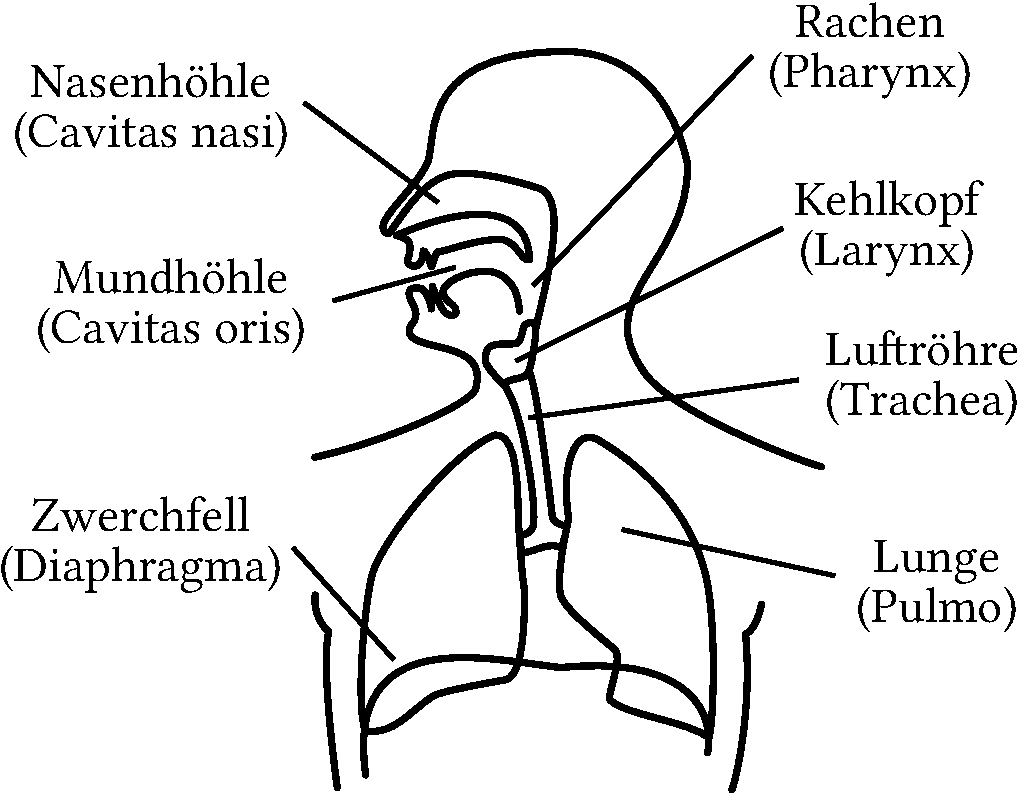
\includegraphics[height=0.7\textheight]{\GRAPHPATH/ueberblick}
\end{frame}

\begin{frame}
  {Mundraum}
  \pause
  \centering
  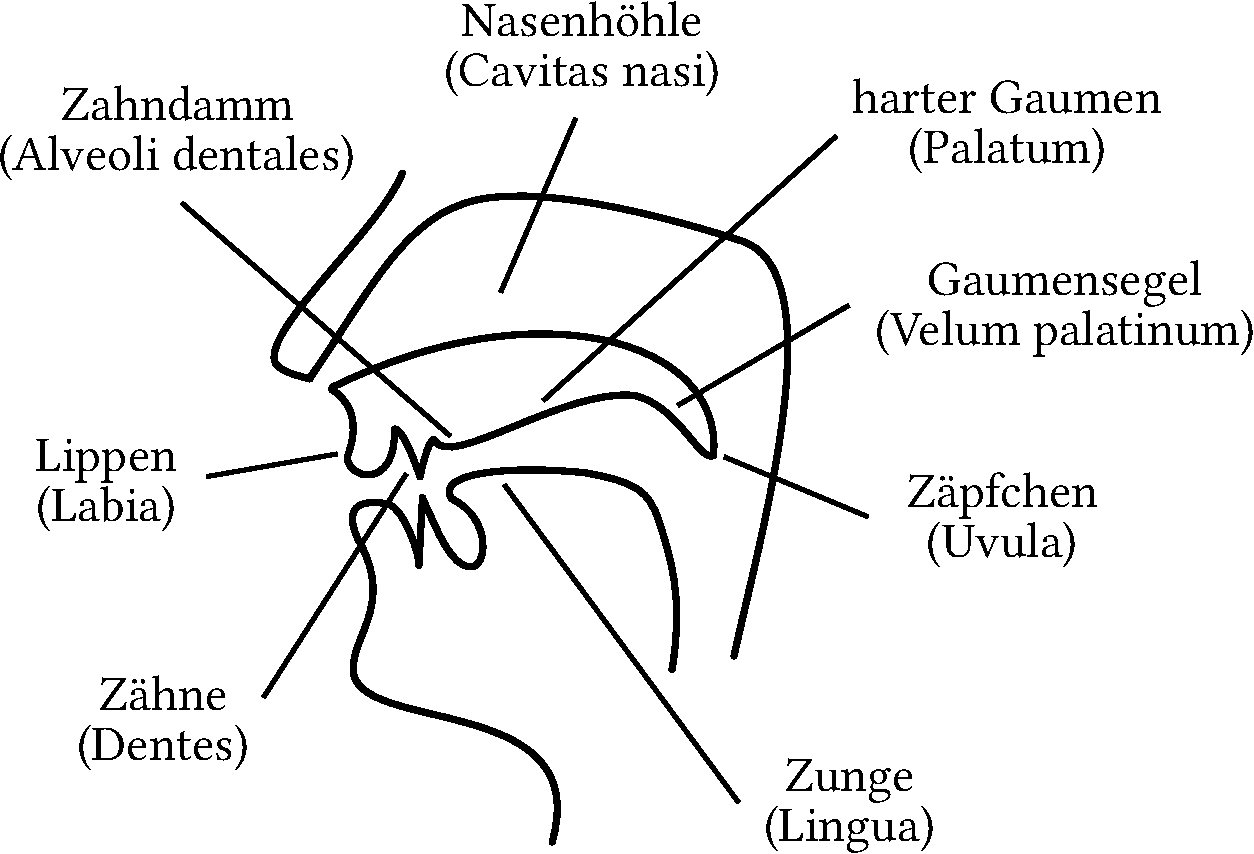
\includegraphics[height=0.7\textheight]{\GRAPHPATH/mundraum}
\end{frame}

\begin{frame}
  {Artikulationsarten | Konsonanten}
  \pause
    \begin{exe}
      \ex \alert{P}ole, \alert{B}ohle; \alert{T}ank, \alert{D}ank; \alert{g}ilt, \alert{k}illt
      \pause
      \ex \alert{F}ee, \alert{w}eh; hei\alert{ß}er, hei\alert{s}er; schli\alert{ch}, \alert{J}ubel; Ba\alert{ch}, \alert{R}une
      \pause
      \ex \alert{Pf}anne; \alert{Z}irkus; Ma\alert{tsch}
      \pause
      \ex \alert{M}us; \alert{N}uss; Go\alert{ng}
    \end{exe}
    \pause
    \Large
    \begin{itemize}
      \item[\ding{220}] \alert{Stimmhaftigkeit}
    \end{itemize}
\end{frame}


\begin{frame}
  {Artikulationsarten | Konsonanten}
  \pause
  \begin{exe}
    \ex \alert{P}a\alert{pp}e, \alert{b}e\alert{b}auen
    \pause
    \ex \alert{T}in\alert{t}e, \alert{d}ul\alert{d}en
    \pause
    \ex \alert{K}na\alert{ck}, \alert{g}e\alert{g}en
    \pause
    \ex Cha\alert{?}ot (Chaos)
    \ex \alert{?}Anfang, \alert{?}über, \alert{?}ohne, \alert{?}Uhr, \dots
  \end{exe}
    \pause
    \Large
    \begin{itemize}
      \item[\ding{220}] \alert{Plosive}
    \end{itemize}
\end{frame}


\begin{frame}
  {Artikulationsarten | Konsonanten}
  \pause
  \begin{exe}
    \ex \alert{f}ün\alert{f}, \alert{w}ehe
    \pause
    \ex Bu\alert{s}, \alert{S}ahne
    \pause
    \ex Bä\alert{ch}e, \alert{J}och
    \pause
    \ex Ba\alert{ch}e, \alert{R}asen
  \end{exe}
    \pause
    \Large
    \begin{itemize}
      \item[\ding{220}] \alert{Frikative}
    \end{itemize}
\end{frame}

\begin{frame}
  {Artikulationsarten | Konsonanten}
  \pause
  \begin{exe}
    \ex \alert{Pf}anne, To\alert{pf} 
    \pause
    \ex \alert{Z}ange, Schli\alert{tz}
    \pause
    \ex Ma\alert{tsch} (\alert{Ch}ips)
    \pause
    \ex (\alert{Dsch}ungel)
  \end{exe}
    \pause
    \Large
    \begin{itemize}
      \item[\ding{220}] \alert{Affrikaten}
    \end{itemize}
\end{frame}

\begin{frame}
  {Artikulationsarten | Konsonanten}
  \pause
  \begin{exe}
    \ex \alert{L}icht, Ba\alert{ll}
  \end{exe}
    \pause
    \Large
    \begin{itemize}
      \item[\ding{220}] \alert{Approximanten}
    \end{itemize}
    \Zeile
  \pause
  \begin{exe}
    \ex \alert{M}aus, Bau\alert{m}
    \pause
    \ex \alert{N}ase, Ki\alert{nn}
    \pause
    \ex Ri\alert{ng}
  \end{exe}
    \pause
    \Large
    \begin{itemize}
      \item[\ding{220}] \alert{Nasale}
    \end{itemize}
\end{frame}


\begin{frame}
  {Artikulationsarten | Vokale}
  \pause
  \begin{exe}
    \ex T\alert{ie}r, T\alert{ü}r; g\alert{u}t
    \pause
    \ex w\alert{e}nig, Fl\alert{ö}te; H\alert{o}se
    \pause
    \ex k\alert{ä}me
    \pause
    \ex B\alert{a}d
    \Zeile
    \pause
    \ex K\alert{i}nd, M\alert{ü}ndel; B\alert{u}s
    \pause
    \ex k\alert{ä}mme, k\alert{ö}nnen; Sch\alert{o}ck
    \pause
    \ex T\alert{a}nne
    \Zeile
    \pause
    \ex s\alert{ei}, Pf\alert{au}, H\alert{eu}
    \Zeile
    \pause
    \ex Tüt\alert{e}, b\alert{e}sonders, Eh\alert{e}, \dots
  \end{exe}
\end{frame}


\begin{frame}
  {Artikulationsarten}
  \pause
  \centering 
  \resizebox{0.9\textwidth}{!}{
  \begin{tikzpicture}[every text node part/.style={align=center}]
    \node (UeVok) at (0,0)  {\textbf{Vokale}\\(prototypisch\\silbisch)};
    \node (UeApr) at (2.5,2)  {Approximanten};
    \node (UeNas) at (5,2)  {Nasale};
    \node (UeFri) at (7.5,2)  {Frikative};
    \node (UeAfr) at (10,2) {Affrikaten};
    \node (UePlo) at (12.5,2)  {Plosive};

    \node (UeSon) at (0,4) {\textbf{Sonoranten}\\(Klanglaute)};
    \node (UeObs) at (12.5,4) {\textbf{Obstruenten}\\(Geräuschlaute)};

    \node (UeKon) at (12.5,0) {\textbf{Konsonanten}\\(prototypisch\\nicht silbisch)};

    \draw (UeSon) to (UeVok);
    \draw [bend left] (UeSon) to (UeApr);
    \draw [bend left] (UeSon) to (UeNas);

    \draw (UeObs) to (UePlo);
    \draw [bend right] (UeObs) to (UeFri);
    \draw [bend right] (UeObs) to (UeAfr);

    \draw [bend right] (UeApr) to (UeKon);
    \draw [bend right] (UeNas) to (UeKon);
    \draw (UePlo) to (UeKon);
    \draw [bend right] (UeFri) to (UeKon);
    \draw [bend right] (UeAfr) to (UeKon);
  \end{tikzpicture}}
\end{frame}

\section{Artikulationsorte}

\begin{frame}
  {Konsonanten an verschiedenen Orten}
  \onslide<+->
  \onslide<+->
  \begin{exe}
    \ex \alert{P}a\alert{pp}e, \alert{B}irne, \alert{M}ulch
    \onslide<+-> \alert{| Bilabiale (Lippen)}
    \onslide<+->
    \ex \alert{F}ahne, \alert{W}itz, \alert{Pf}usch
    \onslide<+-> \alert{| Labiodentale (Lippe-Zunge)}
    \onslide<+->
    \ex \alert{T}raum, \alert{d}ort, Mi\alert{s}t, \alert{s}ing, \alert{Z}under, \alert{L}uft, \alert{n}och
    \onslide<+-> \alert{| Alveolare (Zahndamm)}
    \onslide<+->
    \ex Bu\alert{sch}, \alert{Tsch}echisch
    \onslide<+-> \alert{| Palatoalveolare}
    \onslide<+->
    \ex schle\alert{ch}t, \alert{J}unge
    \onslide<+-> \alert{| Palatale (Gaumen)}
    \onslide<+->
    \ex Ro\alert{ck}, \alert{G}abe, Kli\alert{ng}e
    \onslide<+-> \alert{| Velare (weicher Gaumen)}
    \onslide<+->
    \ex wa\alert{ch}, \alert{r}ütteln
    \onslide<+-> \alert{| Uvulare (Zäpfchen)}
    \onslide<+->
    \ex \alert{?}offen, \alert{h}och
    \onslide<+-> \alert{| Laryngale (Kehlkopf)}
  \end{exe}
\end{frame}


\begin{frame}
  {Artilulationsorte | Konsonanten}
  \centering
  \resizebox{0.7\textwidth}{!}{
  \begin{tabular}{rccccccccc}
    \toprule
    \multicolumn{1}{c}{} & \Sw{\textbf{bilabial}} & \Sw{\textbf{labiodental}} & \Sw{\textbf{alveolar}} & \Sw{\textbf{palatoalveolar}} & \Sw{\textbf{palatal}} & \Sw{\textbf{velar}} & \Sw{\textbf{uvular}} & \Sw{\textbf{laryngal}} \\
    \midrule
    \textbf{stl.\ Plosiv} & p &  & t &  &  & k &  & ʔ \\
    \textbf{sth.\ Plosiv} & b &  & d &  &  & g &  &  \\
    \textbf{stl.\ Frikativ} &  & f & s & ʃ & ç &  & χ & h \\
    \textbf{sth.\ Frikativ} &  & v & z &  & ʝ &  & ʁ &  \\
    \textbf{stl.\ Affrikate} &  & p͡f & t͡s & t͡ʃ &  &  &  &  \\
    \textbf{lateraler Approximant} &  &  & l &  &  &  &  &  \\
    \textbf{Nasal} & m &  & n &  &  & ŋ &  &  \\
    \bottomrule
  \end{tabular}  
  }
\end{frame}


\begin{frame}[fragile]
  {Artiklulationsorte | Vokale}
  \begin{center}
  \resizebox{0.5\textwidth}{!}{
  \begin{tikzpicture}[scale=2.5,baseline=default]
    \large
    \tikzset{
      vowel/.style={fill=white, anchor=mid, text depth=0ex, text height=1ex},
      dot/.style={circle,fill=black,minimum size=0.4ex,inner sep=0pt,outer sep=-1pt},
    }

    \coordinate (hf) at (0,2); % high front
    \coordinate (hb) at (2,2); % high back
    \coordinate (lf) at (1,0); % low front
    \coordinate (lb) at (2,0); % low back
    \def\V(#1,#2){barycentric cs:hf={(3-#1)*(2-#2)},hb={(3-#1)*#2},lf={#1*(2-#2)},lb={#1*#2}}

    % Chart key (vorne -- hinten).
    \draw [{Latex[round]}-] (\V (-.25,0))   -- (\V (-.25,.5)) node [above left] {\footnotesize vorne};
    \draw [-{Latex[round]}] (\V (-.25,1.5)) -- (\V (-.25,2))  node [above left] {\footnotesize hinten};
    \path (\V (-.25,1)) node[above] {\footnotesize zentral};

    % Chart key (hoch--tief).
    \draw [{Latex[round]}-] (\V (0,-.25)) -- +(270:.5cm)  node [above right,rotate=90] (vokaltrapez1) {\footnotesize hoch};
    \draw [{Latex[round]}-] (\V (3,-2.5)) -- +(270:-.5cm) node [above left,rotate=90] (vokaltrapez2) {\footnotesize tief};
    \path (\V (1.5,-1)) node[above,rotate=90] {\footnotesize mittel};

    % Grid. 
    \draw [gray, thick] (\V(0,0)) -- (\V(0,2));
    \draw [gray, thick] (\V(1,0)) -- (\V(1,2));
    \draw [gray, thick] (\V(2,0)) -- (\V(2,2));
    \draw [gray, thick] (\V(3,0)) -- (\V(3,2));
    \draw [gray, thick] (\V(0,0)) -- (\V(3,0));
    \draw [gray, thick] (\V(0,1)) -- (\V(3,1));
    \draw [gray, thick] (\V(0,2)) -- (\V(3,2));

    % Unrounded-rounded pairs.
    \path (\V(0,0))     node[vowel, left]     {i} node[vowel, right] (y) {y} node[dot] {};
    \path (\V(0.5,0.5)) node[vowel, left]     {ɪ} node[vowel, right] (Y) {ʏ} node[dot] {};
    \path (\V(1,0))     node[vowel, left]     {e} node[vowel, right] (e) {ø} node[dot] {};
    \path (\V(2,0))     node[vowel, left] (E) {ɛ} node[vowel, right] (ee) {œ} node[dot] {};

    % Unpaired symbols.
    \path (\V(1.5,1))    node [vowel] (schwa)  {ə};
    \path (\V(2.5,1))    node [vowel] (schwaa) {ɐ};
    \path (\V(3,1))      node [vowel] (a)      {a};
    \path (\V (2,2))     node [vowel] (oo)     {ɔ};
    \path (\V (1,2))     node [vowel] (o)      {o};
    \path (\V (0,2))     node [vowel] (u)      {u};
    \path (\V (0.5,1.5)) node [vowel] (uu)     {ʊ};

    \path (a)  edge [-{Latex[round]}, bend right=15] (oo);
    \path (a)  edge [-{Latex[round]}, bend left=15]  (E);
    \path (oo) edge [-{Latex[round]}, bend right=15] (ee);
  \end{tikzpicture}
  }
  \end{center}
\end{frame}




\section{Besonderheiten im Deutschen | Ausblick Phonologie}

\begin{frame}
  {Endrand-Desonorisierung}
  \pause
  \begin{exe}
    \ex\label{ex:auslautverhaertung011}
    \begin{xlist}
      \ex{\label{ex:auslautverhaertung012} weck [vɛk]}
      \ex{\label{ex:auslautverhaertung013} Weg [veːk]}
      \ex{\label{ex:auslautverhaertung014} Weges [veːgəs]}
    \end{xlist}
  \pause
    \ex\label{ex:auslautverhaertung015}
    \begin{xlist}
      \ex{\label{ex:auslautverhaertung016} bat [baːt]}
      \ex{\label{ex:auslautverhaertung017} Bad [baːt]}
      \ex{\label{ex:auslautverhaertung018} Bades [baːdəs]}
    \end{xlist}
  \pause
    \ex\label{ex:auslautverhaertung019}
    \begin{xlist}
      \ex{\label{ex:auslautverhaertung020} Flop [flɔp]}
      \ex{\label{ex:auslautverhaertung021} Lob [loːp]}
      \ex{\label{ex:auslautverhaertung022} Lobes [loːbəs]}
    \end{xlist}
  \end{exe}
\end{frame}


\begin{frame}
  {Silbische Nasale und Liquiden}
  \pause
  \begin{exe}
    \ex\label{ex:silbischenasaleundapproximanten023}
    \begin{xlist}
      \ex{laufen [la͡ɔfn̩]~\slash~[la͡ɔfən]}
      \ex{haben [habm̩]~\slash~[habən]}
      \ex{kriegen [kʁiːgŋ̩]~\slash~[kʁiːgən]}
      \ex{rotem [ʁoːtm̩]~\slash~[ʁoːtəm]}
      \ex{Bündel [bʏndl̩]~\slash~[bʏndəl]}
    \end{xlist}
  \end{exe}
\end{frame}

\begin{frame}
  {\textit{r}-Laute}
  \pause
  \begin{exe}
    \ex\label{ex:orthographischesr030}
    \begin{xlist}
      \ex{Tier [ti͡ɐ], Tür [ty͡ɐ]}
      \ex{Kirche [kɪ͡əçə], Bürde [bʏ͡ədə]}
      \ex{nur [nu͡ɐ]}
      \ex{Bursche [bʊ͡əʃə]}
      \ex{der [de͡ɐ], Stör [ʃtø͡ɐ]}
      \ex{Chor [ko͡ɐ]}
      \ex{gern [gɛ͡ən], Börse [bœ͡əzə]}
      \ex{Korn [kɔ͡ən]}
      \ex{Bar [ba͡ə]}
      \ex{knarr [kna͡ə]}
    \end{xlist}
  \end{exe}
\end{frame}


\begin{frame}[fragile]
  {Sekundäre Diphthonge}
  \begin{center}
  \resizebox{0.5\textwidth}{!}{
  \begin{tikzpicture}[scale=3,baseline=default]
    \large
    \tikzset{
    vowel/.style={fill=white, anchor=mid, text depth=0ex, text height=1ex},
    dot/.style={circle,fill=black,minimum size=0.4ex,inner sep=0pt,outer sep=-1pt},
    }

    \coordinate (hf) at (0,2); % high front
    \coordinate (hb) at (2,2); % high back
    \coordinate (lf) at (1,0); % low front
    \coordinate (lb) at (2,0); % low back
    \def\V(#1,#2){barycentric cs:hf={(3-#1)*(2-#2)},hb={(3-#1)*#2},lf={#1*(2-#2)},lb={#1*#2}}

    % Chart key (vorne -- hinten).
    \draw [{Latex[round]}-] (\V (-.25,0)) -- (\V (-.25,.5))  node [above left] {\footnotesize vorne};
    \draw [-{Latex[round]}] (\V (-.25,1.5)) -- (\V (-.25,2)) node [above left] {\footnotesize hinten};
    \path (\V (-.25,1)) node[above] {\footnotesize zentral};

    % Chart key (hoch--tief).
    \draw [{Latex[round]}-] (\V (0,-.25)) -- +(270:.5cm)  node [above right,rotate=90] (vokaltrapez1) {\footnotesize hoch};
    \draw [{Latex[round]}-] (\V (3,-2.5)) -- +(270:-.5cm) node [above left,rotate=90] (vokaltrapez2) {\footnotesize tief};
    \path (\V (1.5,-1)) node[above,rotate=90] {\footnotesize mittel};

    % Grid.
    \draw [gray, thick] (\V(0,0)) -- (\V(0,2));
    \draw [gray, thick] (\V(1,0)) -- (\V(1,2));
    \draw [gray, thick] (\V(2,0)) -- (\V(2,2));
    \draw [gray, thick] (\V(3,0)) -- (\V(3,2));
    \draw [gray, thick] (\V(0,0)) -- (\V(3,0));
    \draw [gray, thick] (\V(0,1)) -- (\V(3,1));
    \draw [gray, thick] (\V(0,2)) -- (\V(3,2));

    % Unrounded-rounded pairs.
    \path (\V(0,0))     node[vowel, left] {i} node [vowel, right] (y)  {y} node [dot] {};
    \path (\V(0.5,0.5)) node[vowel, left] {ɪ} node [vowel, right] (Y)  {ʏ} node [dot] {};
    \path (\V(1,0))     node[vowel, left] {e} node [vowel, right] (e)  {ø} node [dot] {};
    \path (\V(2,0))     node[vowel, left] {ɛ} node [vowel, right] (ee) {œ} node [dot] {};

    % Unpaired symbols.
    \path (\V(1.5,1))    node [vowel] (schwa)  {ə};
    \path (\V(2.5,1))    node [vowel] (schwaa) {ɐ};
    \path (\V(3,1))      node [vowel] (a)      {a};
    \path (\V (2,2))     node [vowel] (oo)     {ɔ};
    \path (\V (1,2))     node [vowel] (o)      {o};
    \path (\V (0,2))     node [vowel] (u)      {u};
    \path (\V (0.5,1.5)) node [vowel] (uu)     {ʊ};

    % Connections.
    \path (y) edge  [-{Latex[round]}, bend right=3]  (schwaa);
    \path (e) edge  [-{Latex[round]}, bend right=10] (schwaa);
    \path (ee) edge [-{Latex[round]}, bend left=20]  (schwa);
    \path (a) edge  [-{Latex[round]}, bend right=40] (schwa);
    \path (oo) edge [-{Latex[round]}, bend right=20] (schwa);
    \path (o) edge  [-{Latex[round]}, bend left=15]  (schwaa);
    \path (u) edge  [-{Latex[round]}, bend left=10]  (schwaa);
    
    \draw [-{Latex[round]}]             (Y)  -- (schwa);
    \draw [-{Latex[round]}, bend right] (uu) -- (schwa);
  \end{tikzpicture}
  }
  \end{center}
\end{frame}



\ifdefined\TITLE
  \section{Nächste Woche | Überblick}

  \begin{frame}
    {Semesterplan}
    \begin{enumerate}
      \item Graphematik und Schreibprinzipien
      \item Wiederholung -- Phonetik
      \item \alert{Wiederholung -- Phonologie}
      \item Phonographisches Schreibprinzip -- Konsonanten
      \item Phonographisches Schreibprinzip -- Vokale
      \item Silben und Dehnungsschreibungen
      \item Eszett, Dehnung und Konstanz
      \item Spatien und Majuskeln
      \item Komma
      \item Punkt und sonstige Interpunktion
    \end{enumerate}
  \end{frame}
\fi

  \let\subsection\section\let\section\woopsi
  
  \section{03. Wiederholung -- Phonologie}
  \let\woopsi\section\let\section\subsection\let\subsection\subsubsection
  \begin{frame}
  {Übersicht}
  \pause
  \begin{itemize}[<+->]
    \item \alert{Segmente} als Einheiten der Phonetik\slash Phonologie
    \item nicht alle Segmente überall: \alert{Verteilungen}
    \item Endrand-Desonorisierung, r-Vokalisierung, \textit{ich}\slash\textit{ach}-Laute usw.\\
      und \alert{Ableitung} phonetischer Formen aus lexikalischen Formen
    \item längbare, betonbare und unbetonbare Vokale
      \Zeile
    \item \citet[Abschnitt~5.1]{Schaefer2018b}
    \item zusätzliche Literatur: \citet{Eisenberg2013a}
  \end{itemize}
\end{frame}


\begin{frame}
  {Segmente}
  \pause
  \begin{itemize}[<+->]
    \item Transkriptionen: \textit{Tier} [ti͡ɐ], \textit{Tür} [ty͡ɐ], \textit{rotem} [ʁoːtəm],\\
      \textit{Lob} [loːp], \textit{Bades} [baːdəs], \textit{Pfanne} [p͡fanə], \textit{Osten} [ʔɔstən]
      \vspace{\baselineskip}
    \item Warum gibt es die Basiszeichen im IPA, die es gibt? (a, ə, ɪ, ʔ, p, ʁ usw.)
      \begin{itemize}
        \item \alert{artikulatorische Untrennbarkeit}
        \item \alert{kein autonomes Verhalten potentieller Teile}
      \end{itemize}
      \vspace{\baselineskip}
    \item Sind p͡f und a͡ɔ usw.\ ein oder zwei Segmente? 
      \begin{itemize}
        \item artikulatorisch trennbar
        \item autonomes Verhalten?
        \item eigentlich eine phonologische Frage → Verteilungen
      \end{itemize}
  \end{itemize}
\end{frame}

\begin{frame}
  {Verteilungen: Beispiele}
  \pause
  \begin{exe}
    \ex
      \begin{xlist}
        \ex Tod [\alert{t}oːt], Kot [\alert{k}oːt]
        \pause
        \ex Schott [ʃɔ\alert{t}], Schock [ʃɔ\alert{k}]
      \end{xlist}
        \pause
        \ex Hang [ha\alert{ŋ}], *[\orongsch{ŋ}ah]
        \pause
    \ex
      \begin{xlist}
        \ex Sog [\alert{z}oːk], besingen [bə\alert{z}ɪŋən], *[\orongsch{s}oːk]
        \pause
        \ex fließ [fliː\alert{s}], Boss [bɔ\alert{s}], *[fliː\orongsch{z}]
        \pause
        \ex heißer [ha͡ɛ\alert{s}ɐ], heiser [ha͡ɛ\alert{z}ɐ], Base [baː\alert{z}ə], Basse [ba\alert{s}ə], *[ba\orongsch{z}ə]
      \end{xlist}
  \end{exe}
\end{frame}


\begin{frame}
  {Verteilung: Definition}
  \pause
  \Large
  \begin{block}{Verteilung}
    Die Verteilung eines Segments ist die Menge der Umgebungen, in denen es vorkommt.
  \end{block}
  \pause
  \Zeile
  \begin{block}{Kontrast}
    Zwei phonetisch unterschiedliche Segmente bzw.\ Merkmale stehen in einem phonologischen 
  Kontrast, wenn sie eine teilweise oder vollständig übereinstimmende Verteilung haben und dadurch einen lexikalischen bzw.\ grammatischen Unterschied markieren können.
  \end{block}
\end{frame}

\begin{frame}
  {Neutralisierung: Beispiele}
  \pause
  \begin{exe}
    \ex
    \begin{xlist}
      \ex{Weg [veːk], Weges [veːgəs]}
      \pause
      \ex{Bock [bɔk], Bockes [bɔkəs]}
      \pause
    \end{xlist}
    \ex
    \begin{xlist}
      \ex{Bad [baːt], Bades [baːdəs]}
      \pause
      \ex{Blatt [blat], Blattes [blatəs]}
      \pause
    \end{xlist}
    \ex
    \begin{xlist}
      \ex{Lob [loːp], Lobes [loːbəs]}
      \pause
      \ex{Depp [dɛp], Deppen [dɛpən]}
      \pause
    \end{xlist}
    \ex
    \begin{xlist}
      \ex aktiv [ʔaktiːf], aktive [ʔaktiːvə]
      \pause
      \ex tief [tiːf], tiefe [tiːfə]
      \pause
    \end{xlist}
    \ex
    \begin{xlist}
      \ex fies [f"|iːs], fiese [f"|iːzə]
      \pause
      \ex Bus [bʊs], Busse [bʊsə]
      \pause
    \end{xlist}
  \end{exe}
\end{frame}

\begin{frame}
  {Neutralisierung: Definition}
  \pause
  \Large
  \begin{block}{Neutralisierung}
    Eine Neutralisierung ist die Aufhebung eines phonologischen Kontrasts in einer bestimmten Position.    
  \end{block}
\end{frame}

\begin{frame}
  {Das Lexikon (Kapitel 2)}
  \pause
  \large Zum Verständnis der Phonologie ist der linguistische Begriff\\
  des Lexikons eine Grundvoraussetzung.\\
  \Large
  \Zeile
  \pause
  \begin{block}{Lexikon}
    Das \alert{Lexikon} ist die Menge aller Wörter einer Sprache, definiert durch die vollständige Angabe ihrer Merkmale und deren Werte.    
  \end{block}
  \pause
  \Zeile
  \large
  In der Phonologie ist das relevante Merkmal die \alert{Kette von Segmenten}, die ein Wort eindeutig definiert und von allen anderen Wörtern unterscheidbar macht.
\end{frame}

\begin{frame}
  {Muss man ʔ lexikalisch spezifizieren?}
  \pause
  \begin{itemize}[<+->]
    \item{[ʔan], [dan], [kan], [ʁan], [van], [man], [ban]}
    \item{[ʔoːnə], [boːnə], [loːnə], [t͡soːnə], [foːnə], [moːnə], [zoːnə]}
    \item{[ʔe͡ɐt], [ve͡ɐt], [le͡ɐt], [ke͡ɐt], [te͡ɐt], [ge͡ɐt], [he͡ɐt]}
  \end{itemize}
  \Zeile
  \pause
  \begin{itemize}[<+->]
    \item{\alert{[ʔ] kommt immer am Silbenanfang,\\
      wenn sonst kein anderer Konsonant kommt.}}
    \item{[ʔ] ist artikulatorisch und perzeptorisch wenig salient.}
    \item also: nicht lexikalisch, \alert{automatisch einsetzbar}
  \end{itemize}
\end{frame}

\begin{frame}
  {Endrand-Desonorisierung}
  \pause
  \begin{exe}
    \ex
    \begin{xlist}
      \ex{Weg [veː\alert{k}], Weges [veː\alert{g}əs]}
      \ex{Bock [bɔ\alert{k}], Bockes [bɔ\alert{k}əs]}
    \end{xlist}
    \ex
    \begin{xlist}
      \ex{Bad [baː\alert{t}], Bades [baː\alert{d}əs]}
      \ex{Blatt [bla\alert{t}], Blattes [bla\alert{t}əs]}
    \end{xlist}
    \ex
    \begin{xlist}
      \ex{Lob [loː\alert{p}], Lobes [loː\alert{b}əs]}
      \ex{Depp [dɛ\alert{p}], Deppen [dɛ\alert{p}ən]}
    \end{xlist}
    \ex
    \begin{xlist}
      \ex aktiv [ʔaktiː\alert{F}], aktive [ʔaktiː\alert{v}ə]
      \ex tief [tiː\alert{f}], tiefe [tiː\alert{f}ə]
    \end{xlist}
    \ex
    \begin{xlist}
      \ex fies [f"|iː\alert{s}], fiese [f"|iː\alert{z}ə]
      \ex Bus [bʊ\alert{s}], Busse [bʊ\alert{s}ə]
    \end{xlist}
  \end{exe}
  \pause
  \Zeile
  \begin{itemize}
    \item \alert{Aus welcher Form kann man die andere jeweils "`herleiten"'?}
  \end{itemize}
\end{frame}


\begin{frame}
  {Zugrundeliegende Form und Strukturbedingung}
  \pause
  \Large
  \begin{block}{Zugrundeliegende Form}    
    Die zugrundeliegende Form (eines Wortes) ist genau die Folge von Segmenten, die im Lexikon gespeichert wird, und auf die alle zugehörigen phonetischen Formen zurückgeführt werden können.
  \end{block}
  \pause
  \Zeile
  \begin{block}{Strukturbedingungen}
    Die Formen werden ggf. an die phonologischen Strukturbedingungen (die Regularitäten der phonologischen Grammatik) angepasst.    
  \end{block}
\end{frame}

\begin{frame}
  {Architektur der Grammatik und externer Systeme}
  \pause
  \centering
  \resizebox{0.9\textwidth}{!}{
    \begin{tabular}{ccc}
      \toprule
      \multicolumn{2}{c}{\textbf{Grammatik}} & \textbf{Externe Systeme} \\
      \midrule
      \textbf{Lexikon} & \textbf{Phonologie} & \textbf{Phonetik} \\
      \midrule
      /~/& $\Rightarrow$ & [~]\\
      zugrundeliegende Form & Anpassung an Strukturbedingungen & phonetische Realisierung \\
      \bottomrule
    \end{tabular}
  }
\end{frame}

\begin{frame}
  {Also für ʔ und Endrand-Desonorisierung}
  \pause
  \begin{itemize}[<+->]
    \item ʔ
      \begin{itemize}[<+->]
        \item /an/ $\Rightarrow$ [\alert{ʔ}an] 
        \item /oːnə/ $\Rightarrow$ [\alert{ʔ}oːnə]
        \item /e͡ɐt/ $\Rightarrow$ [\alert{ʔ}e͡ɐt]
      \end{itemize}
      \Zeile
    \item Endrand-Desonorisierung
      \begin{itemize}[<+->]
        \item /veː\gruen{g}/ $\Rightarrow$ [veː\alert{k}], /bɔ\gruen{k}/ $\Rightarrow$ [bɔ\alert{k}]
        \item /baː\gruen{d}/ $\Rightarrow$ [baː\alert{k}], /bla\gruen{t}/ $\Rightarrow$ [bla\alert{t}]
        \item /loː\gruen{b}/ $\Rightarrow$ [loː\alert{p}], /dɛ\gruen{p}/ $\Rightarrow$ [dɛ\alert{p}]
        \item /aktiː\gruen{v}/ $\Rightarrow$ [ʔaktiː\alert{f}], /tiː\gruen{f}/ $\Rightarrow$ [tiː\alert{f}]
        \item /fiː\gruen{z}/ $\Rightarrow$ [f"|iː\alert{s}], /bʊ\gruen{s}/ $\Rightarrow$ [bʊ\alert{s}]
      \end{itemize}
  \end{itemize}
\end{frame}


\begin{frame}
  {Endrand-Desonorisierung als Strukturbedingung}
  \pause
  \Large
  Alle \alert{Obstruenten} sind \alert{stimmlos} am \alert{Silbenende}.
\end{frame}


\begin{frame}
  {Verteilung von [ç] und [χ]}
  \pause
  \begin{exe}
    \ex
    \begin{xlist}
      \ex krieche, schlich, Bücher, Küche, Recht, Köche
      \pause
      \ex Tuch, Geruch, hoch, Koch, Schmach, Bach
    \end{xlist}
  \end{exe}
  \pause
  \Zeile
  \Large
  [ç] kann nicht nach nicht-vorderen Vokalen stehen.\\
  Zugrundeliegendes /ç/ wird daher\\
  nach zentralen und hinteren Vokalen\\
  weiter hinten artikuliert, nämlich als [χ].
\end{frame}

\begin{frame}
  {r-Vokalisierung}
  \pause
  \begin{exe}
    \ex
    \begin{xlist}
      \ex \textit{kleiner} [kla͡ɛ.nɐ], \textit{kleinere} [kla͡ɛ.nə.ʁə]
      \pause
      \ex \textit{Bär} [bɛ͡ɐ], \textit{Bären} [bɛː.ʁən]
      \pause
      \ex \textit{knarr} [kna͡ə], \textit{knarre} [kna.ʁə]
    \end{xlist}
  \end{exe}
  \pause
  \Zeile
  \Large
  Zugrundeliegendes /ʁ/ kann nicht am Silbenende\\
  stehen. Es wird in dieser Position als\\
  Schwa-Segment im sekundären Diphthong\\
  realisiert. Nach gespanntem Vokal folgt [ɐ],\\
  nach ungespanntem folgt [ə]. Schwa und /ʁ/\\
  werden zusammen durch [ɐ] substituiert.\\[0.5\baselineskip]
  \pause
  \alert{Gespannt?}
\end{frame}


\begin{frame}[fragile]
  {Erinnerung an die Vokale des Deutschen}
  \begin{center}
  \resizebox{0.6\textwidth}{!}{
  \begin{tikzpicture}[scale=2.5,baseline=default]
    \large
    \tikzset{
      vowel/.style={fill=white, anchor=mid, text depth=0ex, text height=1ex},
      dot/.style={circle,fill=black,minimum size=0.4ex,inner sep=0pt,outer sep=-1pt},
    }

    \coordinate (hf) at (0,2); % high front
    \coordinate (hb) at (2,2); % high back
    \coordinate (lf) at (1,0); % low front
    \coordinate (lb) at (2,0); % low back
    \def\V(#1,#2){barycentric cs:hf={(3-#1)*(2-#2)},hb={(3-#1)*#2},lf={#1*(2-#2)},lb={#1*#2}}

    % Chart key (vorne -- hinten).
    \draw [{Latex[round]}-] (\V (-.25,0))   -- (\V (-.25,.5)) node [above left] {\footnotesize vorne};
    \draw [-{Latex[round]}] (\V (-.25,1.5)) -- (\V (-.25,2))  node [above left] {\footnotesize hinten};
    \path (\V (-.25,1)) node[above] {\footnotesize zentral};

    % Chart key (hoch--tief).
    \draw [{Latex[round]}-] (\V (0,-.25)) -- +(270:.5cm)  node [above right,rotate=90] (vokaltrapez1) {\footnotesize hoch};
    \draw [{Latex[round]}-] (\V (3,-2.5)) -- +(270:-.5cm) node [above left,rotate=90] (vokaltrapez2) {\footnotesize tief};
    \path (\V (1.5,-1)) node[above,rotate=90] {\footnotesize mittel};

    % Grid. 
    \draw [gray, thick] (\V(0,0)) -- (\V(0,2));
    \draw [gray, thick] (\V(1,0)) -- (\V(1,2));
    \draw [gray, thick] (\V(2,0)) -- (\V(2,2));
    \draw [gray, thick] (\V(3,0)) -- (\V(3,2));
    \draw [gray, thick] (\V(0,0)) -- (\V(3,0));
    \draw [gray, thick] (\V(0,1)) -- (\V(3,1));
    \draw [gray, thick] (\V(0,2)) -- (\V(3,2));

    % Unrounded-rounded pairs.
    \path (\V(0,0))     node[vowel, left]     {i} node[vowel, right] (y) {y} node[dot] {};
    \path (\V(0.5,0.5)) node[vowel, left]     {ɪ} node[vowel, right] (Y) {ʏ} node[dot] {};
    \path (\V(1,0))     node[vowel, left]     {e} node[vowel, right] (e) {ø} node[dot] {};
    \path (\V(2,0))     node[vowel, left] (E) {ɛ} node[vowel, right] (ee) {œ} node[dot] {};

    % Unpaired symbols.
    \path (\V(1.5,1))    node [vowel] (schwa)  {ə};
    \path (\V(2.5,1))    node [vowel] (schwaa) {ɐ};
    \path (\V(3,1))      node [vowel] (a)      {a};
    \path (\V (2,2))     node [vowel] (oo)     {ɔ};
    \path (\V (1,2))     node [vowel] (o)      {o};
    \path (\V (0,2))     node [vowel] (u)      {u};
    \path (\V (0.5,1.5)) node [vowel] (uu)     {ʊ};

  \end{tikzpicture}
  }
  \end{center}
\end{frame}


\begin{frame}
  {Länge und Betonung und Vokalqualität im Systemkern}
  \pause
  \centering
  \begin{tabular}{cllp{0.25cm}cll}
    \toprule
    \textbf{gespannt} & \textbf{Beispiel} & \textbf{IPA} & & \textbf{ungespannt} & \textbf{Beispiel} & \textbf{IPA} \\
    \midrule
    i  & \textit{bieten} & biːtən && ɪ & \textit{bitten}  & bɪtən   \\
    y  & \textit{fühlt}  & fyːlt  && ʏ & \textit{füllt}   & fʏlt    \\
    u  & \textit{Mus}    & muːs   && ʊ & \textit{muss}    & mʊs     \\
    e  & \textit{Kehle}  & keːlə  && ɛ & \textit{Kelle}   & kɛlə    \\
    ɛ  & \textit{stähle} & ʃtɛːlə && ɛ & \textit{Ställe}  & ʃtɛlə   \\
    ø  & \textit{Höhle}  & høːlə  && œ & \textit{Hölle}   & hœlə \\
    o  & \textit{Ofen}   & ʔoːfən && ɔ & \textit{offen}   & ʔɔfən   \\
    a  & \textit{Wahn}   & vaːn   && a & \textit{wann}    & van     \\
    \bottomrule
  \end{tabular}\\
  \pause
  \Zeile
  \begin{itemize}[<+->]
    \item Laut\rot{e}, b\rot{e}schreib\rot{e}n, \dots
    \item L\rot{i}thografie, H\rot{y}draulik, B\rot{u}tan, Ph\rot{e}nol, \rot{Ö}nologie, Mes\rot{o}zoon, \dots
  \end{itemize}
\end{frame}

\begin{frame}
  {Gespanntheit im Kernwortschatz}
  \pause
  \Large
  \rot{Im Kernwortschatz sind gespannte Vokale immer\\
  betont und lang.} Zu jedem gespannten Vokal gibt es\\
  einen entsprechenden ungespannten Vokal.\\
  Der ungespannte ist betont oder unbetont,\\
  aber immer kurz.\\
  \Zeile
  \pause
  Die Länge muss also nicht markiert werden, sondern folgt\\
  aus Betonung und Gespanntheit.
\end{frame}

\begin{frame}[fragile]
  {Gespanntheit}
  \pause
  \begin{center}
    \resizebox{0.6\textwidth}{!}{
      \begin{tikzpicture}[scale=3.5,baseline=default]
        \large
        \tikzset{
        vowel/.style={fill=white, anchor=mid, text depth=0ex, text height=1ex},
        vowelgespannt/.style={circle,fill=gray!30, anchor=mid, text depth=0ex, text height=1ex,minimum size=4ex},
        dot/.style={circle,fill=black,minimum size=0.4ex,inner sep=0pt,outer sep=-1pt},
        }

        \coordinate (hf) at (0,2); % high front
        \coordinate (hb) at (2,2); % high back
        \coordinate (lf) at (1,0); % low front
        \coordinate (lb) at (2,0); % low back
        \def\V(#1,#2){barycentric cs:hf={(3-#1)*(2-#2)},hb={(3-#1)*#2},lf={#1*(2-#2)},lb={#1*#2}}

        % Chart key (vorne -- hinten).
        \draw [{Latex[round]}-] (\V (-.25,0)) -- (\V (-.25,.5))  node [above left] {\footnotesize vorne};
        \draw [-{Latex[round]}] (\V (-.25,1.5)) -- (\V (-.25,2)) node [above left] {\footnotesize hinten};
        \path (\V (-.25,1)) node[above] {\footnotesize zentral};

        % Chart key (hoch--tief).
        \draw [{Latex[round]}-] (\V (0,-.25)) -- +(270:.5cm)  node [above right,rotate=90] (vokaltrapez1) {\footnotesize hoch};
        \draw [{Latex[round]}-] (\V (3,-2.5)) -- +(270:-.5cm) node [above left,rotate=90] (vokaltrapez2) {\footnotesize tief};
        \path (\V (1.5,-1)) node[above,rotate=90] {\footnotesize mittel};

        % Grid.
        \draw [gray,thick] (\V(0,0)) -- (\V(0,2));
        \draw [gray,thick] (\V(3,0)) -- (\V(3,2));
        \draw [gray,thick] (\V(0,0)) -- (\V(3,0));
        \draw [gray,thick] (\V(0,2)) -- (\V(3,2));

        \path (\V(0,0))      node[vowelgespannt] (i)   {i};
        \path (\V(0.25,0))   node[vowelgespannt] (y)   {y};
        \path (\V(0.4,0.5))  node[vowel]         (ii)  {ɪ};
        \path (\V(0.65,0.5)) node[vowel]         (yy)  {ʏ};
        \path (\V(1,0))      node[vowelgespannt] (e)   {e};
        \path (\V(1.25,0))   node[vowelgespannt] (oe)  {ø};
        \path (\V(2,0))      node[vowelgespannt] (ee)  {ɛ};
        \path (\V(1.4,0.7))  node[vowel]         (eee) {ɛ̆};
        \path (\V(1.65,0.7)) node[vowel]         (oee) {œ};
        \path (\V(3,1))      node[vowelgespannt] (a)   {a};
        \path (\V(2.5,1))    node[vowel]         (aa)  {ă};
        \path (\V (1,2))     node[vowelgespannt] (o)   {o};
        \path (\V (1.5,1.4)) node[vowel]         (oo)  {ɔ};
        \path (\V (0,2))     node[vowelgespannt] (u)   {u};
        \path (\V (0.5,1.5)) node[vowel]         (uu)  {ʊ};

        \draw (i)  -- (ii);
        \draw (y)  -- (yy);
        \draw (e)  -- (eee);
        \draw (oe) -- (oee);
        \draw (ee) -- (eee);
        \draw (a)  -- (aa);
        \draw (o)  -- (oo);
        \draw (u)  -- (uu);
      \end{tikzpicture}
    }
  \end{center}
\end{frame}


\begin{frame}
  {Und Schwa?}
  \pause
  Warum kommt Schwa (also [ə] und [ɐ]) im System der gespannten\\
  und ungespannten Vokale nicht vor?\\
  \pause
  \Zeile
  \Zeile
  \centering
  \Large
  \alert{Schwa ist nicht betonbar!}
\end{frame}



\begin{frame}
  {Und der erweiterte Wortschatz?}
  \resizebox{0.9\textwidth}{!}{
  \begin{minipage}{\textwidth}
  \begin{exe}
    \ex\label{ex:gespanntheitbetonungundlaenge021}
    \begin{xlist}
      \ex{\label{ex:gespanntheitbetonungundlaenge022} \textit{Idee} [ʔ\rot{i}deː]\\
      \textit{Initiative} [ʔ\rot{i}n\rot{i}t͡sʝatiːvə]\\
        \textit{inspirieren} [ʔɪnsp\rot{i}ʁiːʁən] }
      \ex{\label{ex:gespanntheitbetonungundlaenge023} \textit{Methyl} [m\rot{e}tyːl]\\
        \textit{Québec} [k\rot{e}bɛk]\\
        \textit{integriert} [ʔɪnt\rot{e}gʁi͡ɐt]\\
        \textit{debattieren} [d\rot{e}batiːʁən] }
      \ex{\label{ex:gespanntheitbetonungundlaenge024} \textit{Utopie} [ʔ\rot{u}topiː]\\
        \textit{Uran} [ʔ\rot{u}ʁaːn] }
      \ex{\label{ex:gespanntheitbetonungundlaenge025} \textit{Motiv} [m\rot{o}tiːf]\\
        \textit{politisch} [p\rot{o}liːtɪʃ]\\
        \textit{Phonologie} [f\rot{o}n\rot{o}l\rot{o}giː] }
      \ex{\label{ex:gespanntheitbetonungundlaenge026} \textit{Ökonomie} [ʔ\rot{ø}konomiː]\\
        \textit{manövrieren} [man\rot{ø}vʁiːʁən] }
      \ex{\label{ex:gespanntheitbetonungundlaenge027} \textit{Büro} [b\rot{y}ʁoː]\\
      \textit{Cuvée} [k\rot{y}veː] }
    \end{xlist}
  \end{exe}
  \end{minipage}
  }
\end{frame}

\begin{frame}
  {Gespanntheit im erweiterten Wortschatz}
  \pause
  \Large
  \rot{Im erweiterten Wortschatz sind gespannte Vokale\\
  lang, wenn sie betont sind, und kurz, wenn sie \\
  unbetont sind.} Auch im erweiterten Wortschatz\\
  gibt es keine ungespannten langen Vokale.\\
\end{frame}

\begin{frame}
  {Zugrundeliegende Formen ohne Länge}
  \begin{exe}
    \ex\label{ex:gespanntheitbetonungundlaenge028} \begin{xlist}
      \ex /v\rot{e}g/ $\Rightarrow$ [v\rot{e}ːk]
      \ex /h\rot{ø}lə/ $\Rightarrow$ [h\rot{ø}ːlə]
      \ex /\rot{o}fən/ $\Rightarrow$ [ʔ\rot{o}ːfən]
    \end{xlist}
  \end{exe}
\end{frame}

\ifdefined\TITLE
  \section{Nächste Woche | Überblick}

  \begin{frame}
    {Der ungefähre Semesterplan}
    \begin{enumerate}[<+->]
      \item Graphematik und Schreibprinzipien
      \item Wiederholung -- Phonetik
      \item Wiederholung -- Phonologie
      \item \alert{Phonographisches Schreibprinzip -- Konsonanten}
      \item Phonographisches Schreibprinzip -- Vokale
      \item Silben und Dehnungsschreibungen
      \item Eszett, Dehnung und Konstanz
      \item Spatien und Majuskeln
      \item Komma
      \item Punkt und sonstige Interpunktion
    \end{enumerate}
  \end{frame}
\fi


\ifdefined\TITLE
  \section{Nächste Woche | Überblick}

  \begin{frame}
    {Der ungefähre Semesterplan}
    \begin{enumerate}[<+->]
      \item Graphematik und Schreibprinzipien
      \item \alert{Wiederholung -- Phonetik}
      \item Wiederholung -- Phonologie
      \item Phonographisches Schreibprinzip -- Konsonanten
      \item Phonographisches Schreibprinzip -- Vokale
      \item Silben und Dehnungsschreibungen
      \item Eszett, Dehnung und Konstanz
      \item Spatien und Majuskeln
      \item Komma
      \item Punkt und sonstige Interpunktion
    \end{enumerate}
  \end{frame}
\fi

  \let\subsection\section\let\section\woopsi
  
  \section{04. Phonographisches Schreibprinzip -- Konsonanten}
  \let\woopsi\section\let\section\subsection\let\subsection\subsubsection
  \section{Übersicht}

\begin{frame}
  {Übersicht}
  \pause
  \begin{itemize}[<+->]
    \item Erinnerung | Kernwortschatz
      \Halbzeile
    \item Inventar der Konsonantenzeichen im Kern
      \Halbzeile
    \item phonographisches Schreibprinzip
      \Halbzeile
    \item Phonologie und Graphematik
  \end{itemize}
\end{frame}

\begin{frame}
  {Erinnerung | der Kernwortschatz I}
  \pause
  Was war nochmal der Kernwortschatz?\\
  \Halbzeile
  \pause
  \begin{itemize}[<+->]
    \item Wörter, für die \alert{die weitreichenden Generalisierungen gelten}
    \item = Wörter und Wortklassen mit \alert{hoher Typenhäufigkeit}
    \item \rot{nicht} die "`häufigen Wörter"' (= Tokenhäufigkeit)
    \item \rot{nicht} die Erbwörter (aber Erbwörter meistens im Kern)
  \end{itemize}
\end{frame}

\begin{frame}
  {Erinnerung | der Kernwortschatz II}
  \pause
  Was war nochmal der Kernwortschatz?\\
  \Halbzeile
  \pause
  \begin{itemize}[<+->]
    \item Kern-Substantive: Einsilbler (im Plural Trochäus) oder Trochäus
    \item warum gerade Substantive so zentral?\\
      \alert{mit Abstand die mächtigste Wortklasse}
      \Halbzeile
    \item \rot{Missverständnis}: Kern\slash Peripherie klar abgegrenzt
    \item je höher die Typenhäufigkeit, desto kerniger
    \item periphere Wörter, Konstruktionen usw.\ \alert{nicht weniger grammatisch}
  \end{itemize}
\end{frame}


\section{Konsonanten}

\begin{frame}
  {Terminologie | Di- und Trigraphen}
  \onslide<+->
  \begin{itemize}[<+->]
    \item Digraphen | zwei Zeichen für ein Segment\\
      \Halbzeile
      \alert{<ch>} für [ç] bzw.\ [χ]\\
      \onslide<+->
      \Halbzeile
      Was ist mit \alert{<pf>}?
    \Zeile
    \item Trigraphen | drei Zeichen für ein Segment\\
      \Halbzeile 
      \alert{<sch>} für [ʃ]
    \Zeile
    \item In ihrer Distribution gekoppelte Zeichen?\\
      \Halbzeile
      \alert{<qu>} für [kv]?
  \end{itemize}
\end{frame}

\begin{frame}
  {Das Inventar (Kern)}
  \onslide<+->
  \begin{itemize}[<+->]
    \item Unigraphen\\
    \Halbzeile
    \alert{k g t d p b}\\
    \onslide<+->
    \alert{z}\\
    \onslide<+->
    \alert{h r j s ß f v w}\\
    \onslide<+->
    \alert{n m l}\\
    \Viertelzeile
    \onslide<+->
    \rot{c q x ?}\\
    \Zeile
  \item Digraphen\\
    \Halbzeile 
    \alert{ng ch pf}
    \onslide<+->
    \rot{qu?}\\
    \Zeile
  \item Trigraphen und Tetragraphen\\
    \Halbzeile 
    \alert{sch tsch}
    \onslide<+->
    \rot{chs?}\\
  \end{itemize}
\end{frame}

\begin{frame}
  {Besondere Doppelkonsonanz}
  \onslide<+->
  \begin{itemize}[<+->]
    \item Reguläre Doppelkonsonanz\\
    \Halbzeile
    \alert{ck tt pp rr ss ff nn mm ll}\\
    \Zeile
    \item Besondere Doppelkonsonanz\\
    \Halbzeile
    \rot{gg dd bb}\\
    \Zeile
    \item Was ist eigentlich mit \alert{<tz>}?
  \end{itemize}
\end{frame}

\begin{frame}
  {Phonographisches Schreibprinzip}
  \onslide<+->
  \onslide<+->
  Versuch: "`Jedes Segment wird durch einen Graphen\\
  (ggf.\ Digraphen usw.) verschriftet."'\\
  \onslide<+->
  \Zeile
  \begin{exe}
    \ex{} [k] \alert{K}ind [g] \alert{G}enau
    \ex{} [t] \alert{T}ante [d] \alert{d}anke
    \ex{} [p] \alert{P}aar [b] \alert{B}ar 
    \ex{} [t͡s] \alert{Z}unge
    \ex{} [h] \alert{H}and [r] \alert{r}ot [j] \alert{j}ung [f] \alert{F}inger [w] \alert{W}anne
    \ex{} [n] \alert{N}ase [m] \alert{M}und [l] \alert{L}ippe
  \end{exe}
\end{frame}


\begin{frame}
  {Problem 1 | Endrand-Desonorisierung}
  \onslide<+->
  \onslide<+->
  \begin{exe}
    \ex Bu\alert{g} [k] --- Bu\alert{g}es [g]
    \ex Ba\alert{d} [t] --- Ba\alert{d}es [d]
    \ex Lo\alert{b} [p] --- Lo\alert{b}es [b]
    \ex bra\alert{v} [f] --- bra\alert{v}er [v]
    \Halbzeile
    \ex besonders: el\alert{f} [f] --- El\alert{f}er [v]
  \end{exe}
  \onslide<+->
  \Zeile
  \alert{Ein Graph} entspricht \alert{zwei Artikulationen}.\\
  \alert{stimmhaft -- stimmlos} \grau{je nach Position in der Silbe}
\end{frame}


\begin{frame}
  {Problem 2 | <ch>}
  \onslide<+->
  \onslide<+->
  \begin{exe}
    \ex schli\alert{ch} [ç]
    \ex Ba\alert{ch} [χ]
  \end{exe}
  \onslide<+->
  \Zeile
  \alert{Ein Graph} entspricht \alert{zwei Artikulationen}.\\
  \alert{Artikulation weiter vorne bzw.\ hinten} \grau{nach vorderen\slash nicht-vorderen Vokalen}
\end{frame}

\begin{frame}
  {Problem 3 | g-Spirantisierung}
  \onslide<+->
  \onslide<+->
  \begin{exe}
    \ex weni\alert{g} [ç]
    \ex weni\alert{g}er [g]
  \end{exe}
  \onslide<+->
  \Zeile
  \alert{Ein Graph} entspricht \alert{zwei Artikulationen}.\\
  \alert{Plosiv vs.\ Frikativ} \grau{je nach Umgebung (Silbenauslaut, vorangehendes /ɪ/)}
\end{frame}

\begin{frame}
  {Problem 4 | r-Vokalisierungen}
  \onslide<+->
  \onslide<+->
  \begin{exe}
    \ex Tie\alert{r} [ti͡ɐ] -- Tie\alert{r}e [ti͡əʁə]
    \ex Cho\alert{r} [ko͡ɐ] --- Chö\alert{r}e [køʁə]
    \ex kna\alert{rr} [kna͡ə] --- kna\alert{rr}en [knaʁən]
  \end{exe}
  \onslide<+->
  \Zeile
  \alert{Ein Graph} entspricht \alert{zwei Artikulationen}.\\
  \alert{[ʁ] oder [ə] bzw.\ [ɐ]} \grau{im Silbenanlaut- bzw.\ auslaut}
\end{frame}

\begin{frame}
  {Phonologie, nicht Phonetik}
  \onslide<+->
  \onslide<+->
  Alle genannten "`Ausnahmen"' zeigen \alert{phonologische Prozesse},\\
  also Anpassungen an Strukturbedingungen des Deutschen!\\
  \onslide<+->
  \Zeile
  Das phonographische Prinzip | Die \alert{(Konsonanten)graphen} entsprechen\\
  je einem \alert{zugrundeliegenden Segment}.
\end{frame}

\begin{frame}
  {Ordnung total: die Konsonantenzeichen}
  \pause
  \centering
  \resizebox{0.375\textwidth}{!}{
    \begin{tabular}{lll}
      \toprule
      \textbf{Segment} & \textbf{Buchstabe(n)} & \textbf{Beispielwörter} \\
      \midrule
     p & p & \textit{Plan} \\
     b & b & \textit{Baum}, \textit{Trab} \\
     p͡f & pf & \textit{Pfad} \\
     f & f & \textit{Fahrt} \\
     v & w & \textit{Wand} \\
     m & m & \textit{Mus} \\
     t & t & \textit{Tau} \\
     d & d & \textit{Dach}, \textit{Bild}\\
     t͡s & z & \textit{Zeit} \\
     \rot{s} & \rot{s} & \textit{Los} \\
     \rot{z} & \rot{s} & \textit{Sau} \\
     ʃ & sch & \textit{Schiff} \\
     n & n & \textit{Not}, \textit{Klang} \\
     l & l & \textit{Lob} \\
     ç & ch & \textit{Blech}, \textit{Wacht} \\
     ʝ & j & \textit{Jahr} \\
     k & k & \textit{Kiel} \\
     g & g & \textit{Gans}, \textit{Weg}, \textit{König} \\
     ʁ & r & \textit{Ritt}, \textit{Tür} \\
     h & h & \textit{Herz} \\
      \bottomrule
    \end{tabular}
  }
\end{frame}

\begin{frame}
  {Invarianz der Konsonantenzeichen}
  \pause
  \alert{Wir schreiben, wie unsere zugrundeliegenden Formen aussehen.}\\
  \pause
  \Zeile
  \centering
  \resizebox{0.9\textwidth}{!}{
    \begin{tabular}{lp{0.15cm}lp{0.15cm}llp{0.15cm}llp{0.15cm}l}
      \toprule
      \textbf{zugr.} && \textbf{Buch-} && \multicolumn{2}{l}{\textbf{phonetische}}    && \multicolumn{2}{l}{\textbf{phonologische}} && \textbf{phonetische} \\
      \textbf{Segm.} && \textbf{stabe(n)} && \multicolumn{2}{l}{\textbf{Realisierungen}} && \multicolumn{2}{l}{\textbf{Schreibungen}}  && \textbf{Schreibung} \\
      \midrule
      b && b && ba͡ɔm & loːp && \textit{Baum} & \textit{Lob} && *\textit{Lop} \\
      d && d && daχ & ʁɪnt && \textit{Dach} & \textit{Rind} && *\textit{Rint} \\
      n && n && naχt & klaŋ && \textit{Nacht} & \textit{Klang} && *\textit{Klaŋ} \\
      ç && ch && lɪçt & vaχt && \textit{Licht} & \textit{Wacht} && *\textit{Waχt} \\
      g && g && gans & køːnɪç && \textit{Gans} & \textit{König} && *\textit{Könich} \\
      ʁ && r && ʁuːm & to͡ɐ && \textit{Ruhm} & \textit{Tor} && *\textit{Toe} \\
      \bottomrule
    \end{tabular}
  }
  \Zeile
  \pause
  \begin{itemize}[<+->]
    \item einige Substitutionsphänome (anlautendes /kv/ als \textit{qu} usw.)
    \item \alert{Das Problem mit den \textit{s}-Schreibungen wird noch gelöst!}
  \end{itemize}
\end{frame}



\ifdefined\TITLE
  \section{Nächste Woche | Überblick}

  \begin{frame}
    {Der ungefähre Semesterplan}
    \begin{enumerate}[<+->]
      \item Graphematik und Schreibprinzipien
      \item Wiederholung -- Phonetik
      \item Wiederholung -- Phonologie
      \item Phonographisches Schreibprinzip -- Konsonanten
      \item \alert{Phonographisches Schreibprinzip -- Vokale}
      \item Silben und Dehnungsschreibungen
      \item Eszett, Dehnung und Konstanz
      \item Spatien und Majuskeln
      \item Komma
      \item Punkt und sonstige Interpunktion
    \end{enumerate}
  \end{frame}
\fi


  \let\subsection\section\let\section\woopsi
  
  \section{05. Phonographisches Schreibprinzip -- Vokale}
  \let\woopsi\section\let\section\subsection\let\subsection\subsubsection
  \section{Übersicht}

\begin{frame}
  {Übersicht}
  \onslide<+->
  \begin{itemize}[<+->]
    \item Vokale im Kernwortschatz
    \item Vokale in der Peripherie
      \Halbzeile
    \item System der Vokalzeichen
    \item Ausblick Dehnungsschreibungen
    \item System der Diphthongschreibungen
  \end{itemize}
\end{frame}

\section{Gespanntheit}

\begin{frame}[fragile]
  {Gespanntheit}
  \pause
  \begin{center}
    \resizebox{0.5\textwidth}{!}{
      \begin{tikzpicture}[scale=3.5,baseline=default]
        \large
        \tikzset{
        vowel/.style={fill=white, anchor=mid, text depth=0ex, text height=1ex},
        vowelgespannt/.style={circle,fill=gray!30, anchor=mid, text depth=0ex, text height=1ex,minimum size=4ex},
        dot/.style={circle,fill=black,minimum size=0.4ex,inner sep=0pt,outer sep=-1pt},
        }

        \coordinate (hf) at (0,2); % high front
        \coordinate (hb) at (2,2); % high back
        \coordinate (lf) at (1,0); % low front
        \coordinate (lb) at (2,0); % low back
        \def\V(#1,#2){barycentric cs:hf={(3-#1)*(2-#2)},hb={(3-#1)*#2},lf={#1*(2-#2)},lb={#1*#2}}

        % Chart key (vorne -- hinten).
        \draw [{Latex[round]}-] (\V (-.25,0)) -- (\V (-.25,.5))  node [above left] {\footnotesize vorne};
        \draw [-{Latex[round]}] (\V (-.25,1.5)) -- (\V (-.25,2)) node [above left] {\footnotesize hinten};
        \path (\V (-.25,1)) node[above] {\footnotesize zentral};

        % Chart key (hoch--tief).
        \draw [{Latex[round]}-] (\V (0,-.25)) -- +(270:.5cm)  node [above right,rotate=90] (vokaltrapez1) {\footnotesize hoch};
        \draw [{Latex[round]}-] (\V (3,-2.5)) -- +(270:-.5cm) node [above left,rotate=90] (vokaltrapez2) {\footnotesize tief};
        \path (\V (1.5,-1)) node[above,rotate=90] {\footnotesize mittel};

        % Grid.
        \draw [gray,thick] (\V(0,0)) -- (\V(0,2));
        \draw [gray,thick] (\V(3,0)) -- (\V(3,2));
        \draw [gray,thick] (\V(0,0)) -- (\V(3,0));
        \draw [gray,thick] (\V(0,2)) -- (\V(3,2));

        \path (\V(0,0))      node[vowelgespannt] (i)   {i};
        \path (\V(0.25,0))   node[vowelgespannt] (y)   {y};
        \path (\V(0.4,0.5))  node[vowel]         (ii)  {ɪ};
        \path (\V(0.65,0.5)) node[vowel]         (yy)  {ʏ};
        \path (\V(1,0))      node[vowelgespannt] (e)   {e};
        \path (\V(1.25,0))   node[vowelgespannt] (oe)  {ø};
        \path (\V(2,0))      node[vowelgespannt] (ee)  {ɛ};
        \path (\V(1.4,0.7))  node[vowel]         (eee) {ɛ̆};
        \path (\V(1.65,0.7)) node[vowel]         (oee) {œ};
        \path (\V(3,1))      node[vowelgespannt] (a)   {a};
        \path (\V(2.5,1))    node[vowel]         (aa)  {ă};
        \path (\V (1,2))     node[vowelgespannt] (o)   {o};
        \path (\V (1.5,1.4)) node[vowel]         (oo)  {ɔ};
        \path (\V (0,2))     node[vowelgespannt] (u)   {u};
        \path (\V (0.5,1.5)) node[vowel]         (uu)  {ʊ};

        \draw (i)  -- (ii);
        \draw (y)  -- (yy);
        \draw (e)  -- (eee);
        \draw (oe) -- (oee);
        \draw (ee) -- (eee);
        \draw (a)  -- (aa);
        \draw (o)  -- (oo);
        \draw (u)  -- (uu);
      \end{tikzpicture}
    }
  \end{center}
\end{frame}

\begin{frame}
  {Vokale im Kernwortschatz}
  \onslide<+->
  \onslide<+->
  \alert{Gespannt} \orongsch{$\rightarrow$ betont und lang}\\
  \Viertelzeile
  \onslide<+->
  \begin{exe}
    \ex \textit{Tüte} /t\alert{y}tə/ $\Rightarrow$ [ˈt\orongsch{yː}.tə]\\
    \ex \textit{Magen} /m\alert{a}gən/ $\Rightarrow$ [ˈm\orongsch{aː}.gən]\\
    \ex \textit{vermietete} /fəʁm\alert{i}tətə/ $\Rightarrow$ [fɐ.ˈm\orongsch{iː}.tə.tə]\\
    \ex \textit{weniger} /v\alert{e}nɪgəʁ/ $\Rightarrow$ [ˈv\orongsch{eː}.nɪ.gɐ]\\
  \end{exe}
  \onslide<+->
  \Zeile
  \alert{Ungespannt} | \gruen{betont oder unbetont} \orongsch{$\rightarrow$ kurz}\\
  \Viertelzeile
  \begin{exe}
    \ex \textit{Sitte} /z\alert{ɪ}tə/ $\Rightarrow$ [ˈz\orongsch{ɪ}ṭə]\\
    \ex \textit{untersetzt} /\tuerkis{ʊ}ntəʁz\alert{ɛ}t͡st/ $\Rightarrow$ [ʔʊn.tɐ.ˈz\orongsch{ɛ}t͡st]\\
    \ex \textit{motzte} /m\alert{ɔ}t͡stə/ $\Rightarrow$ [ˈm\orongsch{ɔ}t͡s.tə]\\
    \ex \textit{unglaublich} /\alert{ʊ}ngla͡ɔblɪç/ $\Rightarrow$ [ʔ\orongsch{ʊ}n.ˈgla͡ɔb.lɪç]\\
  \end{exe}
\end{frame}

\begin{frame}
  {Gespanntheit im Kernwortschatz}
  \onslide<+->
  \onslide<+->
  \large
  \alert{Im Kernwortschatz sind gespannte Vokale immer\\
  betont und lang.} Zu jedem gespannten Vokal gibt es\\
  einen entsprechenden ungespannten Vokal.\\
  Der ungespannte ist betont oder unbetont,\\
  aber immer kurz.\\
  \Zeile
  \onslide<+->
  Die Länge muss also nicht markiert werden, sondern folgt\\
  aus Betonung und Gespanntheit.\\
  \Zeile
  \onslide<+->
  Trochäus-Regel plus Morphologie machen außerdem\\
  den Akzentsitz vorhersagbar!
\end{frame}

\begin{frame}
  {Vorhersagbarkeit des Akzentsitzes I}
  \onslide<+->
  \onslide<+->
  Wieso Trochäus-Regel + Morphologie = Akzentsitz?\\
  \onslide<+->
  \Zeile
  \begin{itemize}[<+->]
    \item \orongsch{Simplex}
      \Halbzeile
    \begin{itemize}[<+->]
      \item \textit{Mut} /mut/ \ensuremath{\Rightarrow} [ˈmuːt]\\
        Im Kern-Einsilber-Stamm: Akzent auf der \alert{einen Silbe}
        \Halbzeile
      \item \textit{Mitte} /mɪte/ \ensuremath{\Rightarrow} [ˈmɪṭə]\\
        Im Kern-Zweisilbler-Stamm: \alert{Trochäus}
        \Halbzeile
      \item \textit{wenigere} /venɪgəʁə/ \ensuremath{\Rightarrow} [ˈveː.nɪ.gə.ʁə]\\
        In längeren Flexionsformen: \alert{Stammakzent} bleibt
    \end{itemize}
  \end{itemize}
\end{frame}


\begin{frame}
  {Vorhersagbarkeit des Akzentsitzes II}
  \onslide<+->
  \onslide<+->
  Wieso Trochäus-Regel + Morphologie = Akzentsitz?\\
  \onslide<+->
  \Halbzeile
  \begin{itemize}[<+->]
    \item \orongsch{Derivate}
    \begin{itemize}[<+->]
      \item \textit{be:end-en} /bəɛndən/ \ensuremath{\Rightarrow} [bə.\blau{ˈʔɛn}.dən]
      \item \textit{unter:scheid-en} /ʊntəʁʃa͡ɛdən/ \ensuremath{\Rightarrow} [ʔʊn.tɐ.\blau{ˈʃa͡ɛ}.dən]
      \item \textit{ge:leg-en} /gəlegən/ \ensuremath{\Rightarrow} [gə.\blau{ˈleː}.gən]
      \item \textit{Eigen:heit} /a͡ɛgənha͡ɛt/ \ensuremath{\Rightarrow} [\blau{ˈʔa͡ɛ}.gən.ha͡ɛt]
      \item \textit{umfahren} /ʊmfaʁən/ \ensuremath{\Rightarrow} [\gruen{ˈʔʊm}.faː.ʁən]
      \item \textit{Unterschied} /ʊntəʁʃid/ \ensuremath{\Rightarrow} [\rot{ˈʔʊn}.tɐ.ʃiːt]
      \item \textit{Faselei} /fazəla͡ɛ/ \ensuremath{\Rightarrow} [faː.zə.\orongsch{ˈla͡ɛ}]
        \Halbzeile
      \item Fast alle Affixe lassen den Akzent auf dem \blau{Stamm}.
      \item \gruen{Verbpartikeln} (nicht Verbpräfixe) ziehen den Akzent an.
      \item \rot{Verpräfixe} ziehen in der Nominalisierung ebenfalls den Akzent an.
      \item Wenige \orongsch{Affixe} ziehen den Akzent an.
    \end{itemize}
  \end{itemize}
\end{frame}

\begin{frame}
  {Vorhersagbarkeit des Akzentsitzes III}
  \onslide<+->
  \onslide<+->
  Wieso Trochäus-Regel + Morphologie = Akzentsitz?\\
  \onslide<+->
  \Halbzeile
  \begin{itemize}[<+->]
    \item \orongsch{Komposita}
    \begin{itemize}[<+->]
      \item \textit{Tankstelle} /tănkʃtɛlə/ \ensuremath{\Rightarrow} [\blau{ˈtaŋk}.ʃtɛḷə]
      \item \textit{Tankstellenwart} /tănkʃtɛlənvaʁt/ \ensuremath{\Rightarrow} [\blau{ˈtaŋk}.ʃtɛḷən.va͡ət]
      \item \textit{Tankstellenwartausbildung} /tănkʃtɛlənvaʁta͡ʊsbɪldʊng/ \ensuremath{\Rightarrow} [\blau{ˈtaŋk}.ʃtɛḷən.va͡ət.ʔa͡ɔs.bɪl.dʊŋ]
        \Halbzeile
      \item Der Akzent bleibt immer uf dem Erstglied.
      \item \grau{Nebenakzente liegen auf den anderen Gliedern.}
    \end{itemize}
  \end{itemize}
\end{frame}

\begin{frame}
  {Fremdwortschatz mit freiem Akzentsitz}
  \resizebox{0.7\textwidth}{!}{
  \begin{minipage}{\textwidth}
    \begin{tabular}{lll}
      \textit{Idee} & /\rot{i}d\gruen{ˈe}/ & [ʔ\rot{i}.ˈd\gruen{eː}]\\
      \textit{Initiative} & /\rot{i}n\rot{i}t͡sʝ\rot{a}t\gruen{ˈi}v\grau{ə}/ & [ʔ\rot{i}.n\rot{i}.t͡sʝ\rot{a}.ˈt\gruen{iː}.v\grau{ə}]\\
      \textit{inspirieren} & /\blau{ɪ}nsp\rot{i}ʁ\gruen{ˈi}ʁ\grau{ə}n/ & [ʔɪn.sp\rot{i}.ˈʁ\gruen{iː}.ʁ\grau{ə}n] \\
      
      \textit{Methyl} & /m\rot{e}t\gruen{ˈy}l/ & [m\rot{e}.ˈt\gruen{yː}l]\\
      \textit{Québec} & /k\rot{e}b\gruen{ˈɛ}k/ & [k\rot{e}.ˈbɛk]\\
      \textit{integriert} & /\blau{ɪ}nt\rot{e}gʁ\gruen{ˈi}ʁt/ & [ʔɪn.t\rot{e}.ˈgʁi͡ɐt]\\
      \textit{debattieren} & /d\rot{e}b\rot{a}t\gruen{ˈi}ʁ\grau{ə}n/ & [d\rot{e}.ba.ˈt\gruen{iː}.ʁ\grau{ə}n] \\
      
      \textit{Utopie} & /\rot{u}t\rot{o}p\gruen{ˈi}/ & [ʔ\rot{u}.to.ˈp\gruen{iː}]\\
      \textit{Uran} & /\rot{u}ʁ\gruen{ˈa}n/ & [ʔ\rot{u}.ˈʁ\gruen{aː}n] \\
      
      \textit{Motiv} & /m\rot{o}t\gruen{ˈi}v/ & [m\rot{o}.ˈt\gruen{iː}f]\\
      \textit{politisch} & /p\rot{o}l\gruen{ˈi}t\blau{ɪ}ʃ/ & [p\rot{o}.ˈl\gruen{iː}.t\blau{ɪ}ʃ]\\
      \textit{Phonologie} & /f\rot{o}n\rot{o}l\rot{o}g\gruen{ˈi}/ & [f\rot{o}.n\rot{o}.l\rot{o}.ˈg\gruen{iː}] \\
      
      \textit{Ökonomie} & /\rot{ø}k\rot{o}n\rot{o}m\gruen{ˈi}/ & [ʔ\rot{ø}.ko.no.ˈm\gruen{iː}]\\
      \textit{manövrieren} & /m\rot{a}n\rot{ø}vʁ\gruen{ˈi}ʁ\grau{ə}n/ & [ma.n\rot{ø}.ˈvʁ\gruen{iː}.ʁ\grau{ə}n] \\
      
      \textit{Büro} & /b\rot{y}r\gruen{ˈo}/ & [b\rot{y}.ˈʁ\gruen{oː}]\\
      \textit{Cuvée} & /k\rot{y}v\gruen{ˈe}/ & [k\rot{y}.ˈv\gruen{eː}] \\
    \end{tabular}
  \end{minipage}
  }\\
  \Halbzeile
  \onslide<+->
  \footnotesize \rot{gespannt + unbetont $\rightarrow$ kurz} | \gruen{gespannt + betont $\rightarrow$ lang} | \\
  \blau{ungespannt + kurz (betont oder unbetont)} | \grau{Schwa, immer unbetont und immer kurz}\\
  \Halbzeile
  Peripherie | Der einzige relevante Unterschied: \rot{Es gibt unbetonte gespannte\\
  (und damit kurze) Vokale.} Der Akzentsitz muss lexikalisch spezifiziert sein.\\
\end{frame}


\begin{frame}
  {Gespanntheit im erweiterten Wortschatz}
  \pause
  \Large
  \rot{Im erweiterten Wortschatz sind gespannte Vokale\\
  lang, wenn sie betont sind, und kurz, wenn sie \\
  unbetont sind.} Auch im erweiterten Wortschatz\\
  gibt es keine ungespannten langen Vokale.\\
\end{frame}

\section{Vokalzeichen}

\begin{frame}
  {Ordnung naja: Vokalzeichen}
  \pause
  \centering
  \scalebox{0.8}{%
    \begin{tabular}{lp{0.5cm}llp{0.25cm}ll}
      \toprule
      \multirow{2}{*}{\textbf{Buchstabe}} && \multicolumn{2}{l}{\textbf{Segment}} && \multicolumn{2}{l}{\textbf{Segment}} \\
       && \textbf{gespannt} & \textbf{Beispiel} && \textbf{ungespannt} & \textbf{Beispiel} \\
      \midrule
      i  && i  & \textit{Igel} && ɪ & \textit{Licht} \\
      ü  && y  & \textit{Rübe} && ʏ & \textit{Rücken} \\
      u  && u  & \textit{Mut} && ʊ & \textit{Butter} \\
      e  && e  & \textit{Mehl} && ɛ̆ & \textit{Bett} \\
      ö  && ø & \textit{Höhle} && œ & \textit{Löffel} \\
      o  && o  & \textit{Ofen} && ɔ & \textit{Motte} \\
      ä  && ɛ  & \textit{Gräte} && ɛ̆ & \textit{Säcke} \\
      a  && a  & \textit{Wal} && ă & \textit{Wall} \\
      \bottomrule
    \end{tabular}
  }
    \Zeile
    \pause
    \begin{itemize}[<+->]
      \item \alert{für gespannte\slash ungespannte Vokalpaare nur je ein Zeichen}
      \item außerdem \textit{e}→/ɛ̆/ und \textit{ä}→/ɛ̆/
      \item "`speter"'-Dialekte zusätzlich \textit{e}→/e/ und \textit{ä}→/e/
        \Halbzeile
      \item \alert{Diphthonge} brechen zusätzlich das phonematische Prinzip
    \end{itemize}
\end{frame}


\begin{frame}[fragile]
  {Gespanntheit in "`speter"'-Dialekten}
  \begin{center}
    \resizebox{0.5\textwidth}{!}{
      \begin{tikzpicture}[scale=3.5,baseline=default]
        \large
        \tikzset{
        vowel/.style={fill=white, anchor=mid, text depth=0ex, text height=1ex},
        vowelgespannt/.style={circle,fill=gray!30, anchor=mid, text depth=0ex, text height=1ex,minimum size=4ex},
        dot/.style={circle,fill=black,minimum size=0.4ex,inner sep=0pt,outer sep=-1pt},
        }

        \coordinate (hf) at (0,2); % high front
        \coordinate (hb) at (2,2); % high back
        \coordinate (lf) at (1,0); % low front
        \coordinate (lb) at (2,0); % low back
        \def\V(#1,#2){barycentric cs:hf={(3-#1)*(2-#2)},hb={(3-#1)*#2},lf={#1*(2-#2)},lb={#1*#2}}

        % Chart key (vorne -- hinten).
        \draw [{Latex[round]}-] (\V (-.25,0)) -- (\V (-.25,.5))  node [above left] {\footnotesize vorne};
        \draw [-{Latex[round]}] (\V (-.25,1.5)) -- (\V (-.25,2)) node [above left] {\footnotesize hinten};
        \path (\V (-.25,1)) node[above] {\footnotesize zentral};

        % Chart key (hoch--tief).
        \draw [{Latex[round]}-] (\V (0,-.25)) -- +(270:.5cm)  node [above right,rotate=90] (vokaltrapez1) {\footnotesize hoch};
        \draw [{Latex[round]}-] (\V (3,-2.5)) -- +(270:-.5cm) node [above left,rotate=90] (vokaltrapez2) {\footnotesize tief};
        \path (\V (1.5,-1)) node[above,rotate=90] {\footnotesize mittel};

        % Grid.
        \draw [gray,thick] (\V(0,0)) -- (\V(0,2));
        \draw [gray,thick] (\V(3,0)) -- (\V(3,2));
        \draw [gray,thick] (\V(0,0)) -- (\V(3,0));
        \draw [gray,thick] (\V(0,2)) -- (\V(3,2));

        \path (\V(0,0))      node[vowelgespannt] (i)   {i};
        \path (\V(0.25,0))   node[vowelgespannt] (y)   {y};
        \path (\V(0.4,0.5))  node[vowel]         (ii)  {ɪ};
        \path (\V(0.65,0.5)) node[vowel]         (yy)  {ʏ};
        \path (\V(1,0))      node[vowelgespannt] (e)   {e};
        \path (\V(1.25,0))   node[vowelgespannt] (oe)  {ø};
%        \path (\V(2,0))      node[vowelgespannt] (ee)  {ɛ};
        \path (\V(1.4,0.7))  node[vowel]         (eee) {ɛ̆};
        \path (\V(1.65,0.7)) node[vowel]         (oee) {œ};
        \path (\V(3,1))      node[vowelgespannt] (a)   {a};
        \path (\V(2.5,1))    node[vowel]         (aa)  {ă};
        \path (\V (1,2))     node[vowelgespannt] (o)   {o};
        \path (\V (1.5,1.4)) node[vowel]         (oo)  {ɔ};
        \path (\V (0,2))     node[vowelgespannt] (u)   {u};
        \path (\V (0.5,1.5)) node[vowel]         (uu)  {ʊ};

        \draw (i)  -- (ii);
        \draw (y)  -- (yy);
        \draw (e)  -- (eee);
        \draw (oe) -- (oee);
%        \draw (ee) -- (eee);
        \draw (a)  -- (aa);
        \draw (o)  -- (oo);
        \draw (u)  -- (uu);
      \end{tikzpicture}
    }
  \end{center}
\end{frame}




\begin{frame}
  {Gründe für das System der Vokalzeichen}
  \pause
  \begin{itemize}[<+->]
    \item im Kern: \alert{Kopplung von Gespanntheit, Länge und Betonung}
    \item aber trotzdem \alert{keine zugrundeliegenden Formen} für Gespanntheitspaare
    \item zusammen mit \alert{Silbengelenkschreibung} (s.\,u.) aber\\
      kaum Bedarf an graphematischer Differenzierung
      \Halbzeile
    \item außerdem Entwicklung von \alert{Dehnungsschreibungen}\\
      zur Desambiguierung
    \item \ldots\ weil \alert{Gespanntheit + Akzent → Länge}
      \Halbzeile
    \item trotzdem suboptimal
  \end{itemize}
\end{frame}

\begin{frame}
  {Realisierungen der Dehnungsschreibung}
  \onslide<+->
  \onslide<+->
  Gespanntheitsmarkierung |\\
  \alert{h}, \orongsch{nichts}, \grau{Doppelvokal} oder bei <i> die \alert{<ie>-Schreibung}\\
  \Zeile
  \begin{tabular}{llllll}
    /i/ &           \rot{*<ih>} & \alert{<ie>} & \orongsch{<i>} &          \rot{*<ii>} & \textit{R\alert{ie}men}, \textit{\orongsch{I}gel}, *\textit{Kn\rot{ii}b}, *\textit{Kn\rot{ih}p} \\
    /y/ & \whyte{*}\alert{<üh>} &              & \orongsch{<ü>} &          \rot{*<üü>} & \textit{B\alert{üh}ne}, \textit{m\orongsch{ü}de}, *\textit{B\rot{üü}ke} \\
    /e/ & \whyte{*}\alert{<eh>} &              & \orongsch{<e>} & \whyte{*}\grau{<ee>} & \textit{k\alert{eh}ren}, \textit{w\orongsch{e}nig}, \textit{S\grau{ee}} \\
    /ɛ/ & \whyte{*}\alert{<äh>} &              & \orongsch{<ä>} &          \rot{*<ää>} & \textit{\alert{Äh}re}, \textit{d\orongsch{ä}nisch}, *\textit{S\rot{ää}le} \\
    /ø/ & \whyte{*}\alert{<öh>} &              & \orongsch{<ö>} &          \rot{*<öö>} & \textit{st\alert{öh}nen}, \textit{fl\orongsch{ö}ten}, *\textit{d\rot{öö}fer} \\
    /u/ & \whyte{*}\alert{<uh>} &              & \orongsch{<u>} &          \rot{*<uu>} & \textit{K\alert{uh}le}, \textit{Sch\orongsch{u}le}, *\textit{Kr\rot{uu}fe} \\
    /o/ & \whyte{*}\alert{<oh>} &              & \orongsch{<o>} & \whyte{*}\grau{<oo>} & \textit{L\alert{oh}n}, \textit{B\orongsch{o}den}, \textit{d\grau{oo}f} \\
    /a/ & \whyte{*}\alert{<ah>} &              & \orongsch{<a>} & \whyte{*}\grau{<aa>} & \textit{W\alert{ah}n}, \textit{b\orongsch{a}den}, \textit{\grau{Aa}l} \\
  \end{tabular}\\
  \Zeile 
  \onslide<+->
  <i>, <u> und Umlautgraphen können nicht gedoppelt werden!\\
  Wir kommen zu den "`Dehnungsschreibungen"' noch ausführlich zurück.
\end{frame}

\begin{frame}
  {Diphthongschreibungen (Kern)}
  \onslide<+->
  \onslide<+->
  \begin{itemize}[<+->]
    \item Diphthonge als komplexe Einsegmente
    \item Diphthongzeichen damit \alert{Digraphen}
    \item Achtung | \rot{Lautwert im Diphthong ungleich Lautwert isoliert}
  \end{itemize}
  \onslide<+->
  \Zeile
  \begin{exe}
    \ex \textit{H\gruen{au}s} /h\alert{a͡ɔ}z/ $\rightarrow$ [ˈh\alert{a͡ɔ}s]
    \onslide<+->
    \ex 
    \begin{xlist}
      \ex \textit{M\gruen{ai}s} /m\alert{a͡ɛ}z/ $\rightarrow$ [ˈ\alert{ma͡ɛ}s] 
      \ex \textit{M\gruen{ei}se} /m\alert{a͡ɛ}ze/ $\rightarrow$ [ˈ\alert{ma͡ɛ}.zə] 
    \end{xlist}
    \onslide<+->
    \ex \begin{xlist}
      \ex \textit{Häuser} /h\alert{ɔ͡œ}zəʁ/ $\rightarrow$ [ˈh\alert{ɔ͡œ}.zɐ]
      \ex \textit{Schleuse} /ʃl\alert{ɔ͡œ}zə/ $\rightarrow$ [ˈʃl\alert{ɔ͡œ}.zə] 
    \end{xlist}
  \end{exe}
\end{frame}

\begin{frame}
  {System der Diphthongschreibungen?}
  \onslide<+->
  \onslide<+->
  \begin{center}
    \begin{tabular}{cc}
      \toprule
      \Large mögliche & \Large mögliche \\
      \Large Erstglieder & \Large Zweitglieder \\
      \midrule
      \Large \alert{a (ä) e} & \Large \gruen{i u} \\
      \bottomrule
    \end{tabular}
  \end{center}
  \Zeile
  \begin{itemize}[<+->]
    \item{ }<a> und <e> auch als Doppelvokale\\
      \textit{Haar}, \textit{Saat}, \textit{Waage}\\
      \textit{Beere}, \textit{leer}, \textit{Meer}
      \Halbzeile
    \item{ }<uu> und <ii> selbst in Phantasiewörtern ausgeschlossen\\
      *\textit{Diip}, *\textit{Kiibe}, *\textit{Duut}, *\textit{Kuute}
      \Zeile
    \item eindeutiges \alert{Diphthongsignal}: \alert{<i> und <u> nach Vokalzeichen}
  \end{itemize}
\end{frame}

\begin{frame}
  {Form der Vokalzeichen}
  \onslide<+->
  \onslide<+->
  Es gibt distributionell drei Gruppen von Vokalzeichen.\\
  \Zeile
  \begin{itemize}[<+->]
    \item \alert{<\textit{a}> <\textit{e}> <\textit{o}>}
      \begin{itemize}[<+->]
        \item typische Vokale \alert{ohne Oberlänge}
        \item \ldots\ und \alert{graphisch rund}
      \end{itemize}
      \Halbzeile
    \item \orongsch{<\textit{u}> <\textit{i}>}
      \begin{itemize}[<+->]
        \item partiell atypisch durch \orongsch{geringere graphische Rundheit}
        \item als Zweitglieder im Diphthong \orongsch{näher am Endrand (Coda)}\\
          (graphisch \orongsch{konsonantischer})
        \item \orongsch{nicht verdoppelbar}
        \item{} <ie> Dehnungsschreibung mit prototypischen <e>-Graphen
      \end{itemize}
      \Halbzeile
    \item \rot{<\textit{ä}> <\textit{ö}> <\textit{ü}>}
      \begin{itemize}[<+->]
        \item atypische Vokale durch \rot{Oberlänge}
        \item \rot{nicht verdoppelbar}
      \end{itemize}
  \end{itemize}
\end{frame}

\ifdefined\TITLE
  \section{Nächste Woche | Überblick}

  \begin{frame}
    {Der ungefähre Semesterplan}
    \begin{enumerate}[<+->]
      \item Graphematik und Schreibprinzipien
      \item Wiederholung -- Phonetik
      \item Wiederholung -- Phonologie
      \item Phonographisches Schreibprinzip -- Konsonanten
      \item Phonographisches Schreibprinzip -- Vokale
      \item \alert{Silben und Dehnungsschreibungen}
      \item Eszett, Dehnung und Konstanz
      \item Spatien und Majuskeln
      \item Komma
      \item Punkt und sonstige Interpunktion
    \end{enumerate}
  \end{frame}
\fi

  \let\subsection\section\let\section\woopsi
  
  \section{06. Silben und Dehnungsschreibungen}
  \let\woopsi\section\let\section\subsection\let\subsection\subsubsection
  \section{Übersicht}

\begin{frame}
  {Übersicht}
  \onslide<+->
  \begin{itemize}[<+->]
    \item Silben
    \item Sonorität
    \item Extrasilbizität
    \item Anfangs- und Endrand
    \item Silbengewicht
      \Zeile
    \item Silbengelenke
    \item Schärfungsschreibung als Gelenkschreibung
  \end{itemize}
\end{frame}

\section{Silben}

\begin{frame}
  {Was sind Silben?}
  \pause
  \begin{itemize}[<+->]
    \item genaue Definition schwierig
    \item "`rhythmische Einheiten"' (bzw.\ metrische Einheiten)
      \Zeile
    \item \alert{rein phonologische} Ebene \alert{zwischen Segment und Wort}
    \item eigene \alert{Regularitäten}: Abfolge der Segmente
      \Zeile
    \item \alert{nicht lexikalisch festgelegt}: \textit{klüger} [klyː.g\rot{ɐ}], \textit{klügere} [klyː.g\rot{ə}.\rot{ʁ}ə]
  \end{itemize}
\end{frame}

\begin{frame}[fragile]
  {Silbenstruktur, konstruiert am Einsilbler}
  \pause
  Im Einsilbler:\\
  \begin{itemize}[<+->]
    \item \rot{immer ein Vokal}
    \item \alert{immer mindestens ein Konsonant davor (ggf.\ [ʔ])}
    \item möglicherweise Konsonanten danach\\
      (ohne: \alert{offene} Silbe, mit: \alert{geschlossene} Silbe)
  \end{itemize}
  \Zeile
  \pause
  \begin{center}
    \begin{forest}
      [Silbe, calign=last
        [Anfangsrand, sake, calign=first
          [C][C]
        ]
        [Reim, calign=first
          [Kern, sake, calign=first
            [V]
          ]
          [Endrand, sake, calign=last
            [C][C]
          ]
        ]
      ]
    \end{forest}
  \end{center}
\end{frame}



\begin{frame}[fragile]
  {Sonorität und Sonoritätshierarchie}
  \pause
  \begin{itemize}[<+->]
    \item \textit{Tag}, \textit{Mund}, \textit{Lob}, \textit{Knack}, \textit{grün}, \textit{Klang}, \dots
      \Zeile
    \item Prototypisch:
      \begin{itemize}[<+->]
        \item \alert{Sprechwerkzeuge öffnen und schließen}
        \item \alert{Stimmton geht an und aus.}
      \end{itemize}
      \Zeile
    \item unterschiedliche Öffnungsgrade bei Plosiven, Frikativen,\\
      Nasalen, Liquiden (/ʁ/ /l/), Vokalen korrespondieren mit \alert{Sonorität}
      
  \end{itemize}
  \pause
  \begin{center}
    \begin{tikzpicture}
      \node (min)                             {minimal sonor};
      \node (plo) at ([shift={( 3,0)}]   min) {\textbf{Plosive}};
      \node (fri) at ([shift={( 0,0.5)}] plo) {\textbf{Frikative}};
      \node (nas) at ([shift={( 0,0.5)}] fri) {\textbf{Nasale}};
      \node (liq) at ([shift={( 0,0.5)}] nas) {\textbf{Liquide}};
      \node (vok) at ([shift={( 0,0.5)}] liq) {\textbf{Vokale}};
      \node (max) at ([shift={(-3,0)}]   vok) {maximal sonor};
      \draw [->, thick] (min) to (max);
    \end{tikzpicture}
  \end{center}
\end{frame}


\begin{frame}[fragile]
  {Sonoritätskonturen}
  \pause
  \begin{center}
      \SonDiag[2]{{k/\plo/0, u:/\vok/0}}
  \end{center}
\end{frame}

\begin{frame}[fragile]
  {Sonoritätskonturen}
  \begin{center}
      \SonDiag[2]{{n/\nas/0, i:/\vok/0}}
  \end{center}
\end{frame}

\begin{frame}[fragile]
  {Sonoritätskonturen}
  \begin{center}
      \SonDiag[3]{{k/\plo/0, n/\nas/0, i:/\vok/0}}
  \end{center}
\end{frame}

\begin{frame}[fragile]
  {Sonoritätskonturen}
  \begin{center}
      \SonDiag[3]{{d/\plo/0, ʁ/\liq/0, oː/\vok/0}}
  \end{center}
\end{frame}

\begin{frame}[fragile]
  {Sonoritätskonturen}
  \begin{center}
      \SonDiag[3]{{ʃ/\fri/2, t/\plo/0, e:/\vok/0}}
  \end{center}
\end{frame}

\begin{frame}[fragile]
  {Sonoritätskonturen}
  \begin{center}
      \SonDiag[4]{{ʃ/\fri/2, p/\plo/0, ʁ/\liq/0, y:/\vok/0}}
  \end{center}
\end{frame}

\begin{frame}[fragile]
  {Sonoritätskonturen}
  \begin{center}
      \SonDiag[3]{{ʔ/\plo/0, a/\vok/0, p/\plo/0}}
  \end{center}
\end{frame}

\begin{frame}[fragile]
  {Sonoritätskonturen}
  \begin{center}
      \SonDiag[3]{{ʔ/\plo/0, a/\vok/0, n/\nas/0}}
  \end{center}
\end{frame}

\begin{frame}[fragile]
  {Sonoritätskonturen}
  \begin{center}
      \SonDiag[4]{{ʔ/\plo/0, a/\vok/0, χ/\fri/0, t/\plo/0}}
  \end{center}
\end{frame}

\begin{frame}[fragile]
  {Sonoritätskonturen}
  \begin{center}
      \SonDiag[4]{{ʔ/\plo/0, a/\vok/0, l/\liq/0, m/\nas/0}}
  \end{center}
\end{frame}

\begin{frame}[fragile]
  {Sonoritätskonturen}
  \begin{center}
      \SonDiag[4]{{ʁ/\liq/0, a/\vok/0, p/\plo/0, s/\fri/2}}
  \end{center}
\end{frame}



\begin{frame}[fragile]
  {Extrasilbisch}
  \pause
  \begin{itemize}[<+->]
    \item eingekreist: \alert{Verletzungen der Sonoritätskontur}
    \item Lösung: nicht i.\,e.\,S.\ Bestandteile der Silben
    \item \rot{extrasilbische} Konsonanten
      \Zeile
    \item im Anfangsrand nur: \alert{/ʃ/}
    \item im Endrand nur: \alert{/s/ und /t/}
    \item nur \rot{alveolare Obstruenten} (im weiteren Sinn)
      \Zeile
    \item Ist ein Segement extrasilbisch, sind es auch alle folgenden:
  \end{itemize}
  \pause
  \begin{center}
    \SonDiag[6]{{h/\fri/0, ɛ͡ə/\vok/0, p/\plo/0, s/\fri/2, t/\plo/2, s/\fri/2}}
  \end{center}
\end{frame}

\begin{frame}[fragile]
  {Silbenstruktur mit Extrasilbizität}
  \pause
  \begin{center}
  \SonDiag[8]{{ʃ/\fri/2, t/\plo/0, ʁ/\liq/0, ɔ/\vok/0, l/\liq/0, ç/\fri/0, s/\fri/2, t/\plo/2}}
  \Zeile
  \pause
  \begin{forest}
    [Silbe, calign=last
      [Anfangsrand, sake, calign=child, calign child=2
        [X, edge=dashed][C][C]
      ]
      [Reim, calign=first
        [Kern, sake
          [V]
        ]
        [Endrand, sake, calign=child, calign child=2
          [C][C][X,edge=dashed][X,edge=dashed][X,edge=dashed]
        ]
      ]
    ]
  \end{forest}
  \end{center}
\end{frame}


\begin{frame}
  {Was wo steht: Anfangsrand}
  \pause
  \scalebox{0.75}{\begin{minipage}{\textwidth} 
  \begin{exe}
    \ex Simplex
    \pause
    \begin{xlist}
      \ex Po, Bau, Tau, Deich, Kuh, Gang
      \pause
      \ex Fee, Weh, Schuh, hau, Sau, Joch
      \pause
      \ex Mond, Nacht
      \pause
      \ex Lied, Reh
    \end{xlist}
    \pause
    \ex Duplex
    \pause
    \begin{xlist}
      \ex Qual
      \pause
      \ex Knie, Gnu
      \pause
      \ex \alert{Pracht, Bräu, Trank, Dreh, Krach, Grind}
      \pause
      \ex \alert{Fracht, Wrack}
      \pause
      \ex \alert{Platz, Blau, Klang, Glas}
      \pause
      \ex \alert{Floh}
    \end{xlist}
    \pause
    \ex Mit extrasilbischem Konsonanten
    \pause
    \begin{xlist}
      \ex Span, Stau; Spruch, Streich; Spliss
      \pause
      \ex Schwund
      \pause
      \ex Schmach, Schnee
      \pause
      \ex Schlauch, Schrank
    \end{xlist}
  \end{exe}
  \end{minipage}}
\end{frame}


\begin{frame}
  {Was wo steht: Endrand, duplex}
  \pause
  \scalebox{0.85}{\begin{minipage}{\textwidth} 
  \begin{exe}
    \ex Abt, Akt
    \Zeile
    \pause
    \ex Haft, Knast, Acht
    \Zeile
    \pause
    \ex
    \begin{xlist}
      \ex Bank, Rang(?), Hanf, Mensch, Gans
      \pause
      \ex Lump, Ramsch, Wams
    \end{xlist}
    \Zeile
    \pause
    \ex
    \begin{xlist}
      \ex \alert{Korb, Ort, Mark; Alp, Halt, welk}
      \pause
      \ex \alert{Hort, Dorsch, Lurch; Welt, falsch, Milch}
      \pause
      \ex Darm, Kern; Qualm, Köln
    \end{xlist}
  \end{exe}
  \end{minipage}}
  \Zeile
\end{frame}

\begin{frame}
  {Prototypische komplexe Ränder}
  \pause
  \Zeile
  \Large
  \centering
  Der prototypische komplexe Anfangsrand besteht aus\\
  \alert{einem Obstruenten gefolgt von einem Liquid}.\\
  \Zeile
  \pause
  Der prototypische komplexe Endrand besteht aus\\
  \alert{einem Liquid gefolgt von einem Obstruenten}.\\
  \pause
  \Zeile
  Prototypischer komplexer Anfangsrand und Endrand\\
  sind \alert{spiegelbildlich} aufgebaut.
\end{frame}


\begin{frame}
  {Warum reden wir jetzt gleich vom Silbengewicht?}
  \pause
  Wir erfassen zwei wesentliche Beobachtungen:
  \pause
  \Zeile
  \begin{itemize}[<+->]
    \item Es gibt u.\,a.\ Einschränkungen der Besetzungsmöglichkeiten\\
      des \alert{Endrands}, die von der \alert{Länge des Kern-Vokals} abhängen.
    \item Offene Silben mit kurzem Vokal gibt es (fast) nur mit Schwa.
  \Zeile
\item Diese Beschränkung betrifft also den \alert{Reim}.
  \end{itemize} 
\end{frame}

\begin{frame}
  {Silbengewicht als Beschränkung im Reim}
  \pause
  \Halbzeile
  \begin{center}
  \scalebox{0.8}{
  \begin{tabular}{llll}
    \toprule
                         & \textbf{Kern}        & \textbf{Endrand} & \textbf{Beispiele} \\
    \midrule
    \textbf{einmorig}    & \multirow{2}{*}{/ə/} & & \multirow{2}{*}{{}[ʔeː.ə], [tʁuː.ə]} \\
    (überleicht)         &                      & & \\
    \midrule
    \textbf{zweimorig}   & V & C & {}[ʔap], [knap]\\
    (leicht)             & VV & & {}[bla͡ɔ], [ʃneː], \rot{*[ʃne]} \\
    \midrule
    \textbf{dreimorig}   & V & CC & {}[balt], [ʔɪst], [nakt], \rot{*[baːlk]}, \rot{*[ʔiːmʃ]} \\
    (schwer)             & VV & C & {}[zoːk], [la͡ɔp], \rot{*[baːŋk]}, \rot{*[kvaːlm]} \\
    \bottomrule
  \end{tabular}
  }
  \end{center}
  \pause
  \Zeile
  \raggedright
  \begin{itemize}[<+->]
    \item \alert{Nur der \textbf{Reim} ist für das Silbengewicht relevant!}
    \item überleichte (einmorige) Silben nur mit Schwa\ldots\\
      und in speziellen Umgebungen (siehe unten, Korrektur zu EGBD3) \\
    \item überschwere (vier- oder mehrmorige) Silben \rot{niemals} möglich
  \end{itemize}
\end{frame}


% \begin{frame}
%   {Extrasilbisch II}
%   \pause
%   \scalebox{0.85}{\begin{minipage}{\textwidth} 
%   \begin{exe}
%     \ex Nicht überschwer (also max.\ drei Moren):
%     \begin{xlist}
%       \ex /ăçt/ $\Rightarrow$ [ʔaχt] (\textit{Acht})
%       \pause
%       \ex /lɛ̆st/ $\Rightarrow$ [lɛst] (\textit{lässt})
%       \pause
%       \ex /năkt/ $\Rightarrow$ [nakt] (\textit{nackt})
%       \pause
%       \ex /kʁăçs/ $\Rightarrow$ [kʁaχs] (\textit{Krachs})
%       \pause
%       \ex /ăçt/ $\Rightarrow$ [ʔaχt] (\textit{Acht})
%     \end{xlist}
%     \pause
%     \ex Extrasilbizität wegen drohender Überschwere:
%     \begin{xlist}
%       \ex /lest/ $\Rightarrow$ [leːs+t] (\textit{lest})
%       \pause
%       \ex /ʁuft/ $\Rightarrow$ [ʁuːf+t] (\textit{ruft})
%       \pause
%       \ex /huts/ $\Rightarrow$ [huːt+s] (\textit{Huts})
%       \pause
%       \ex /legt/ $\Rightarrow$ [leːk+t] (\textit{legt})
%       \pause
%       \ex /la͡ɔfs/ $\Rightarrow$ [la͡ɔf+s] (\textit{Laufs})
%       \pause
%       \ex /fʊʁçt/ $\Rightarrow$ [fʊ͡əç+t] (\textit{Furcht})
%       \pause
%       \ex /fɛ̆lʃst/ $\Rightarrow$ [fɛlʃ+st] (\textit{fälschst})
%     \end{xlist}
%   \end{exe}
%   \end{minipage}}
% \end{frame}


\begin{frame}
  {Überleichte Silben mit betonbaren Vokalen?}
  \pause
  Was ist mit:
  \begin{itemize}[<+->]
    \item \rot{[bʊ]} in [ˈbʊ.tɐ]
    \item \rot{[ma]} in [ˈma.t͡ʃə]
    \item \rot{[klɪ]} in [ˈklɪ.ŋə]
  \end{itemize}
  \Zeile
  \centering
  \pause
  \rot{Sind das doch einmorige (überleichte) Silben mit Vollvokal?}\\
  \Zeile
  \pause
  \raggedright
  Dieser Silbentyp tritt nur auf:\\
  \begin{itemize}[<+->]
    \item \alert{in (scheinbar) offenen Silben} (sonst nicht überleicht)
    \item \alert{in der betonten Silbe eines Trochäus}
    \item \alert{vor simplexen Anfangsrändern}
  \end{itemize}
\end{frame}

\begin{frame}
  {Silbengelenke}
  \pause
  Lösung: Die Silben sind \alert{nicht überleicht}, \alert{der Konsonant\\
  an der Silbengrenze gehört zum Endrand der ersten und\\
zum Anfangsrand der zweiten Silbe}.\\
  \pause
  \Zeile
  \begin{center}
  \begin{forest}
    [Wort
      [Silbe, calign=last
        [Anfangsrand, ake
          [m]
        ]
        [Reim, calign=first
          [Kern, ake
            [ɪ]
          ]
          [Endrand, ake, name=ERBaum]
        ]
      ]
      [Silbe, calign=last
        [Anfangsrand, ake
          [t]
          {\draw[-] (.north) -- (ERBaum.south);}
        ]
        [Reim
          [Kern, ake
            [ə]
          ]
        ]
      ]
    ]
  \end{forest}
  \end{center}
\end{frame}

\begin{frame}
  {Silbengelenke}
  \begin{center}
  \SonDiag[4]{{m/\nas/0, ɪ/\vok/0, t/\plo/1, ə/\vok/0}}    
  \end{center}
\end{frame}




\section{Schärfung}


\begin{frame}
  {Das Faszinosum der Schärfungsschreibung}
  \pause
  Dehnungs-\slash Schärfungsschreibungen (Einsilbler\slash trochäischer Zweisilbler)\\
  \Zeile
  \pause
  \centering
  \resizebox{0.85\textwidth}{!}{
    \begin{tabular}{lllllllll}
      \toprule
      & & & \textbf{ɪ} & \textbf{ʊ} & \multicolumn{2}{l}{\LocStrutGrph\textbf{ɛ̆}} & \textbf{ɔ} & \textbf{ă} \\
      \midrule

      \multirow{4}{*}{\rotatebox{90}{\textbf{ungespannt}}}

      & \multirow{2}{*}{\rotatebox{90}{\textbf{offen}}}
      & \textbf{einsilb.}  & \textit{\Nono}  & \textit{\Nono}           & \multicolumn{2}{l}{\LocStrutGrph\textit{\Nono}}         & \textit{\Nono}        & \textit{\Nono}           \\
      && \textbf{zweisilb.}  & \textit{Li.\alert{pp}e} & \textit{Fu.\alert{tt}er}         & \multicolumn{2}{l}{\LocStrutGrph\textit{We.\alert{ck}e}}        & \textit{o.\alert{ff}en}       & \textit{wa.\alert{ck}er}         \\
        & \multirow{2}{*}{\rotatebox{90}{\textbf{gesch.}}}
        & \textbf{einsilb.}  & \textit{Ki\rot{nn}}   & \textit{Schu\rot{tt}}    & \multicolumn{2}{l}{\LocStrutGrph\textit{Be\rot{tt}}}           & \textit{Ro\rot{ck}}         & \textit{Wa\rot{tt}}            \\
        && \textbf{zweisilb.}  & \textit{Rin.de} & \textit{Wun.der}        & \multicolumn{2}{l}{\LocStrutGrph\textit{Wen.de}}        & \textit{pol.ter}      & \textit{Tan.te}          \\

      \midrule

      \multirow{4}{*}{\rotatebox{90}{\textbf{gespannt}}}

      & \multirow{2}{*}{\rotatebox{90}{\textbf{offen}}}
        & \textbf{einsilb.}  & \textit{Knie}   & \textit{Schuh}       & \textit{Schnee, Reh}  & \textit{zäh}          & \textit{roh}          & (\textit{da})            \\
      && \textbf{zweisilb.}  & \textit{Bie.ne} & \textit{Kuh.le, Schu.le} & \textit{we.nig}       & \textit{Äh.re, rä.kel} & \textit{oh.ne, O.fen} & \textit{Fah.ne, Spa.ten} \\

      & \multirow{2}{*}{\rotatebox{90}{\textbf{gesch.}}}
        & \textbf{einsilb.}  & \textit{lieb}  & \textit{Ruhm, Glut}      & \textit{Weg}          & \textit{spät}           & \textit{rot}          & \textit{Tat}             \\
      && \textbf{zweisilb.}  & (\textit{lieb.lich}) & (\textit{lug.te})   & (\textit{red.lich})   & (\textit{wähl.te})     & (\textit{brot.los})   & (\textit{rat.los})       \\

      \midrule
      & & & \textbf{i} & \textbf{u} & \textbf{e} & \textbf{ε} & \textbf{o} & \textbf{a} \\

      \bottomrule
    \end{tabular}
  }
  \Halbzeile\pause
  \begin{itemize}[<+->]
    \item \alert{Schärfungsschreibung im Trochäus nur nach ungespanntem Vokal\\
      in offener Silbe, wenn Anfangsrand der Zweitsilbe konsonantisch}
    \item \ldots\ \rot{und im geschlossenen Einsilbler mit ungespanntem Vokal}
  \end{itemize}
\end{frame}

\begin{frame}
  {Details und oft Übersehenes}
  \pause
  \begin{itemize}[<+->]
    \item \alert{Schärfungsschreibung = Silbengelenkschreibung}
    \item Aber warum dann im Einsilbler (\textit{Kinn}, \textit{Bett}, \textit{Rock})?
      \begin{itemize}[<+->]
        \item Siehe nächste Woche!
      \end{itemize}
      \Halbzeile
    \item Merke: Silbengelenkschreibung nur da, wo auch Silbengelenk:
      \begin{itemize}[<+->]
        \item \alert{zwischen Erst- und Zweitsilbe des Trochäus}
        \item \alert{nach ungespanntem} (=kurzem) \alert{Vokal}
      \end{itemize}
  \end{itemize}
\end{frame}

\begin{frame}
  {Details und oft Übersehenes II}
  \pause
  \begin{itemize}[<+->]
    \item \alert{keine Schärfungsschreibung bei Di- und Trigraphen}
      \begin{itemize}[<+->]
        \item \textit{Esche} [ɛʃ̣ə], \textit{zischen} [t͡sɪʃ̣ən]
        \item \textit{Kachel} [kaχ̣əl], \textit{Zeche} [t͡sɛç̣ə]
        \item \textit{Kringel} [kʁɪŋ̣əl], \textit{Zunge} [t͡sʊŋ̣ə]
      \end{itemize}
      \Halbzeile
    \item \rot{Warum sind stimmhafte Obstruenten im Silbengelenk "`eigentlich"' unmöglich?}
      \begin{itemize}[<+->]
        \item Obstruent auch im Endrand der Erstsilbe: \alert{Endrand-Desonorisierung}
        \item \textit{Kladde}, \textit{Robbe}, \textit{Bagger}, ?\textit{prasseln} [pʁazəln], *\textit{quivveln}
        \item \ldots\ \rot{nicht Kern} (fünf oder sechs Typen, alle niederdeutsch)
      \end{itemize}
  \end{itemize}
\end{frame}

\begin{frame}
  {Überblick über Gelenkschreibungen}
  \onslide<+->
  \onslide<+->
  \centering 
  \scalebox{0.7}{%
  \begin{tabular}{lllll}
    /k/  & k      & \rot{ck}        & \textit{Macke} & [maḳə] \\
    /t/  & t      & \alert{tt}      & \textit{Matte} & [maṭə] \\
    /p/  & p      & \alert{pp}      & \textit{Mappe} & [map̣ə] \\
      &&&\\
    /t͡ʃ/ & tsch ? & \orongsch{tsch} & \textit{Ratsche} & [ʁaṭ͡ʃə] \\
    /t͡s/ & z      & \rot{tz}        & \textit{platzen} & [plat͡sən] \\
    /p͡f/ & pf     & \orongsch{pf}   & \textit{zupfen} & [t͡sʊp͡f̣ən] \\
      &&&\\
    /χ/  & ch     & \orongsch{ch}   & \textit{Bache} & [baχ̣ə] \\
    /r/  & r      & \alert{rr}      & \textit{Knarre} & [knaʁ̣ə] \\
    /ʃ/  & sch    & \orongsch{sch}  & \textit{Esche} & [ʔɛʃ̣ə] \\
    /s/  & s      & \alert{ss}      & \textit{lassen} & [laṣən] \\
    /f/  & f      & \alert{ff}      & \textit{hoffen} & [hɔf̣ən] \\
      &&&\\
    /n/  & n      & \alert{nn}      & \textit{Wanne} & [vaṇə] \\
    /m/  & m      & \alert{mm}      & \textit{Kämme} & [kɛṃə] \\
    /l/  & l      & \alert{ll}      & \textit{knallen} & [knaḷən] \\
      &&&\\
    \grau{/g/} &&&& \\
    \grau{/d/} &&&& \\
    \grau{/b/} &&&& \\
  \end{tabular}%
}
\end{frame}



\ifdefined\TITLE
  \section{Nächste Woche | Überblick}

  \begin{frame}
    {Semesterplan}
    \begin{enumerate}
      \item Graphematik und Schreibprinzipien
      \item Wiederholung -- Phonetik
      \item Wiederholung -- Phonologie
      \item Phonographisches Schreibprinzip -- Konsonanten
      \item Phonographisches Schreibprinzip -- Vokale
      \item Silben und Dehnungsschreibungen
      \item \alert{Eszett, Dehnung und Konstanz}
      \item Spatien und Majuskeln
      \item Komma
      \item Punkt und sonstige Interpunktion
    \end{enumerate}
  \end{frame}
\fi

  \let\subsection\section\let\section\woopsi
  
  \section{07. Eszett, Dehnung und Konstanz}
  \let\woopsi\section\let\section\subsection\let\subsection\subsubsection
  \section{Übersicht}

\begin{frame}
  {Übersicht}
  \onslide<+->
  \begin{itemize}[<+->]
    \item Wozu brauchen wir das \alert{Eszett}?
      \Zeile
    \item \alert{Konstanzprinzip} | Stämme möglichst konstant schreiben
      \Zeile
    \item Fazit | \rot{Kann die Dehnungsschreibung weg?}
  \end{itemize}
\end{frame}


\section{Eszett}

\newcommand{\phopro}{\ensuremath{\Rightarrow}}

\begin{frame}
  {Analyse des Eszett}
  \pause
  \begin{itemize}[<+->]
    \item \alert{Alle Positionen bis auf die \textit{ß}-Umgebung sind herleitbar:}
      \begin{itemize}[<+->]
        \item Wortanlaut (\textit{Sog} [zoːk]): zugrundeliegendes /z/ bleibt [z]
        \item Wortauslaut (\textit{Mus} [muːs]): zugrundeliegendes /z/ würde sowieso [s]\\
          wegen Endrand-Desonorisierung
        \item Wortinneren nach ungespanntem Vokal (\textit{Masse} [maṣə]): \alert{Silbengelenk}\\
          immer stimmlos wegen Endranddesonorisierung (/măzə/ undenkbar)
      \end{itemize}
      \Halbzeile
    \item \alert{Bis hierhin brauchen wir noch kein zugrundeliegendes /s/!}
      \Halbzeile
    \item zugrundeliegendes /s/ \rot{nur für das Wortinnere nach gespanntem Vokal}\\
      \textit{Straße} [ʃtʁaːsə] gegenüber \textit{Hase} [haːzə]
    \item \alert{Und wenn statt /s/ einfach /zz/ zugrundeliegt?}
    \item \alert{Und wenn /zz/ mit \textit{ß} geschrieben wird?}
    \item also: \textit{Bußen} als /buzzən/ \phopro [buːssən]
  \end{itemize}
\end{frame}

\begin{frame}
  {Eszett-Silben und die anderen \textit{s}}
  \pause
  \centering
  {\footnotesize\textit{Busen}:}\hspace{1em}\scalebox{0.55}{%
    \begin{forest}
      for tree={s sep+=1em}
      [Phonologisches Wort, calign=first
        [Silbe, calign=last
          [Ar., ake
            [b]
          ]
          [Reim
            [Kern, ake
              [uː]
            ]
          ]
        ]
        [Silbe, calign=last
          [Ar., ake, baseline
            [z]
          ]
          [Reim, calign=first
            [Kern, ake
              [ə]
            ]
            [Er., ake
              [n]
            ]
          ]
        ]
      ]
    \end{forest}
  }~\pause\hspace{1.5em}{\footnotesize\textit{Bussen}:}\hspace{1em}\scalebox{0.55}{%
    \begin{forest}
      for tree={s sep+=1em}
      [Phonologisches Wort, calign=first
        [Silbe, calign=last
          [Ar., ake
            [b]
          ]
          [Reim, calign=first
            [Kern, ake
              [ʊ]
            ]
            [Er., ake, name=BusenEr]
          ]
        ]
        [Silbe, calign=last
          [Ar., ake, baseline
            [s]
            {\draw[-] (.north) -- (BusenEr.south);}
          ]
          [Reim, calign=first
            [Kern, ake
              [ə]
            ]
            [Er., ake
              [n]
            ]
          ]
        ]
      ]
    \end{forest}
  }\\
  \pause
  \Zeile
  {\footnotesize\textit{Bußen} mit \alert{Endranddesonorisierung} und \orongsch{Assimilation}:}\hspace{1em}\scalebox{0.55}{%  
    \begin{forest}
      for tree={s sep+=1em}
      [Phonologisches Wort, calign=first
        [Silbe, calign=last
          [Ar., ake
            [b]
          ]
          [Reim, calign=first
            [Kern, ake
              [uː]
            ]
            [Er., ake
              [\alert{\textbf{s}}]
            ]
          ]
        ]
        [Silbe, calign=last
          [Ar., ake, baseline
            [\orongsch{\textbf{s}}]
          ]
          [Reim, calign=first
            [Kern, ake
              [ə]
            ]
            [Er., ake
              [n]
            ]
          ]
        ]
      ]
    \end{forest}
  }
\end{frame}


\begin{frame}
  {Schritt für Schritt}
  \pause
  \begin{enumerate}[<+->]
    \item zugrundeliegende Form: \alert{/buzzən/}
    \item Silbifizierung \phopro \{buz\orongsch{.}zən\}
    \item Längung gespannter Vokale \phopro \{b\orongsch{uː}z.zən\}
    \item Endranddesonorisierung \phopro \{buː\orongsch{s}.zən\}
    \item Assimilation des Anfangsrands \phopro \alert{[buːs.}\orongsch{s}\alert{ən]}
  \end{enumerate}
  \pause
  \begin{itemize}[<+->]
    \item Ist die Assimilation ein Taschenspielertrick?
    \item Nein, denn sie findet auch in anderen Fällen statt!
  \end{itemize}
  \pause
  \begin{exe}
    \ex\label{ex:dehnungsundschaerfungsschreibungen024}
    \begin{xlist}
      \ex{\label{ex:dehnungsundschaerfungsschreibungen025} /ɛ̆k\alert{z}ə/ \phopro\ [ʔɛk.\orongsch{s}ə] (\textit{Echse})}
      \pause
      \ex{\label{ex:dehnungsundschaerfungsschreibungen026} /ɛ̆ʁb\alert{z}e/ \phopro\ [ʔɛ͡əp.\orongsch{s}ə] (\textit{Erbse})}
    \end{xlist}
  \end{exe}
  \pause
  \begin{itemize}[<+->]
    \item Also ist das Konsonantenzeichen \textit{s} \rot{nicht} doppelt belegt.
    \item \alert{Es gibt zugrundeliegend nur /z/.}
  \end{itemize}
\end{frame}


\section[Konstanz]{Konstantschreibung}

\begin{frame}
  {Zur Erinnerung: unerklärte Doppelkonsonanten}
  \pause
  \centering
  \resizebox{0.7\textwidth}{!}{
    \begin{tabular}{lllllllll}
      \toprule
      & & & \textbf{ɪ} & \textbf{ʊ} & \multicolumn{2}{l}{\LocStrutGrph\textbf{ɛ̆}} & \textbf{ɔ} & \textbf{ă} \\
      \midrule

      \multirow{4}{*}{\rotatebox{90}{\textbf{ungespannt}}}

      & \multirow{2}{*}{\rotatebox{90}{\textbf{offen}}}
      & \textbf{einsilb.}  & \textit{\Nono}  & \textit{\Nono}           & \multicolumn{2}{l}{\LocStrutGrph\textit{\Nono}}         & \textit{\Nono}        & \textit{\Nono}           \\
      && \textbf{zweisilb.}  & \textit{Li.\alert{pp}e} & \textit{Fu.\alert{tt}er}         & \multicolumn{2}{l}{\LocStrutGrph\textit{We.\alert{ck}e}}        & \textit{o.\alert{ff}en}       & \textit{wa.\alert{ck}er}         \\
        & \multirow{2}{*}{\rotatebox{90}{\textbf{gesch.}}}
        & \textbf{einsilb.}  & \textit{Ki\rot{nn}}   & \textit{Schu\rot{tt}}    & \multicolumn{2}{l}{\LocStrutGrph\textit{Be\rot{tt}}}           & \textit{Ro\rot{ck}}         & \textit{Wa\rot{tt}}            \\
        && \textbf{zweisilb.}  & \textit{Rin.de} & \textit{Wun.der}        & \multicolumn{2}{l}{\LocStrutGrph\textit{Wen.de}}        & \textit{pol.ter}      & \textit{Tan.te}          \\

      \midrule

      \multirow{4}{*}{\rotatebox{90}{\textbf{gespannt}}}

      & \multirow{2}{*}{\rotatebox{90}{\textbf{offen}}}
        & \textbf{einsilb.}  & \textit{Knie}   & \textit{Schuh}       & \textit{Schnee, Reh}  & \textit{zäh}          & \textit{roh}          & (\textit{da})            \\
      && \textbf{zweisilb.}  & \textit{Bie.ne} & \textit{Kuh.le, Schu.le} & \textit{we.nig}       & \textit{Äh.re, rä.kel} & \textit{oh.ne, O.fen} & \textit{Fah.ne, Spa.ten} \\

      & \multirow{2}{*}{\rotatebox{90}{\textbf{gesch.}}}
        & \textbf{einsilb.}  & \textit{lieb}  & \textit{Ruhm, Glut}      & \textit{Weg}          & \textit{spät}           & \textit{rot}          & \textit{Tat}             \\
      && \textbf{zweisilb.}  & (\textit{lieb.lich}) & (\textit{lug.te})   & (\textit{red.lich})   & (\textit{wähl.te})     & (\textit{brot.los})   & (\textit{rat.los})       \\

      \midrule
      & & & \textbf{i} & \textbf{u} & \textbf{e} & \textbf{ε} & \textbf{o} & \textbf{a} \\

      \bottomrule
    \end{tabular}
  }
\end{frame}

\begin{frame}
  {Lösung | Konstanz}
  \begin{itemize}[<+->]
    \item Warum \textit{Kinn}, \textit{Schutt}, \textit{Bett}, \textit{Rock}, \textit{Wattes}?
      \Halbzeile
    \item \alert{nicht unterlassbare Gelenkschreibungen}
      \begin{itemize}[<+->]
        \item \textit{die Ki\alert{nn}e}
        \item \textit{des Schu\alert{tt}es}
        \item \textit{die Be\alert{tt}en}
        \item \textit{die Rö\alert{ck}e}
      \end{itemize}
      \Halbzeile
    \item \alert{Die Schreibungen eines Stamms einander angleichen!} Sonst:
      \begin{itemize}[<+->]
        \item \textit{*Kin --- Kinne}
        \item \textit{Schut --- Schutt}
        \item \textit{Bet --- Betten}
        \item \textit{Rok --- Röcke}
      \end{itemize}
  \end{itemize}
\end{frame}

\begin{frame}
  {Andere Konstantschreibungen}
  \pause
  \begin{itemize}[<+->]
    \item andere Wortklassen
      \begin{itemize}[<+->]
        \item \textit{*plat --- pla\rot{tt} --- pla\alert{tt}er}
        \item \textit{*as --- a\rot{ß} --- a\alert{ß}en}
        \item aber: \textit{las --- lasen}
        \item \textit{*schlizte --- schli\rot{tz}te --- schli\alert{tz}en}
      \end{itemize}
      \Halbzeile
    \item andere Phänomene (nicht Silbengelenk oder \textit{ß})
      \begin{itemize}[<+->]
        \item \textit{*gest --- ge\rot{h}st --- ge\alert{h}en}
        \item \textit{*siest --- sie\rot{h}st --- se\alert{h}en}
        \item \textit{*Reume --- R\rot{äu}me --- R\alert{au}m}
        \item \textit{*leuft --- l\rot{äu}ft --- l\alert{au}fen}
      \end{itemize}
  \end{itemize}
\end{frame}


\section{Schärfung + Konstanz = überflüssige Dehnung}

\begin{frame}
  {Das Kreuz mit der Dehnungsschreibung}
  \pause
  \begin{itemize}[<+->]
    \item Dehnungs-\textit{h} (\textit{Reh}, \textit{Pfahl}) oder Dehnungs-Doppelvokal (\textit{Saat}, \textit{Boot})
    \item speziell bei \textit{i} (dort fast immer): Dehnungs-\textit{e} (\textit{Knie}, \textit{Dieb})
      \Halbzeile
    \item \alert{weitgehend redundant} (erst recht im Kern)
    \item \alert{unsystematisch} (\textit{Lid}, \textit{Lied} usw.)
      \Halbzeile
    \item mangels Systematik: \alert{oft Erwerbsprobleme}
    \item \ldots\ denen kaum systematisch zu begenen ist
  \end{itemize}
\end{frame}

\begin{frame}
  {Erinnerung | Realisierungen der Dehnungsschreibung}
  \onslide<+->
  \onslide<+->
  Gespanntheitsmarkierung |\\
  \alert{h}, \orongsch{nichts}, \grau{Doppelvokal} oder bei <i> die \alert{<ie>-Schreibung}\\
  \Zeile
  \begin{tabular}{llllll}
    /i/ &           \rot{*<ih>} & \alert{<ie>} & \orongsch{<i>} &          \rot{*<ii>} & \textit{R\alert{ie}men}, \textit{\orongsch{I}gel}, *\textit{Kn\rot{ii}b}, *\textit{Kn\rot{ih}p} \\
    /y/ & \whyte{*}\alert{<üh>} &              & \orongsch{<ü>} &          \rot{*<üü>} & \textit{B\alert{üh}ne}, \textit{m\orongsch{ü}de}, *\textit{B\rot{üü}ke} \\
    /e/ & \whyte{*}\alert{<eh>} &              & \orongsch{<e>} & \whyte{*}\grau{<ee>} & \textit{k\alert{eh}ren}, \textit{w\orongsch{e}nig}, \textit{S\grau{ee}} \\
    /ɛ/ & \whyte{*}\alert{<äh>} &              & \orongsch{<ä>} &          \rot{*<ää>} & \textit{\alert{Äh}re}, \textit{d\orongsch{ä}nisch}, *\textit{S\rot{ää}le} \\
    /ø/ & \whyte{*}\alert{<öh>} &              & \orongsch{<ö>} &          \rot{*<öö>} & \textit{st\alert{öh}nen}, \textit{fl\orongsch{ö}ten}, *\textit{d\rot{öö}fer} \\
    /u/ & \whyte{*}\alert{<uh>} &              & \orongsch{<u>} &          \rot{*<uu>} & \textit{K\alert{uh}le}, \textit{Sch\orongsch{u}le}, *\textit{Kr\rot{uu}fe} \\
    /o/ & \whyte{*}\alert{<oh>} &              & \orongsch{<o>} & \whyte{*}\grau{<oo>} & \textit{L\alert{oh}n}, \textit{B\orongsch{o}den}, \textit{d\grau{oo}f} \\
    /a/ & \whyte{*}\alert{<ah>} &              & \orongsch{<a>} & \whyte{*}\grau{<aa>} & \textit{W\alert{ah}n}, \textit{b\orongsch{a}den}, \textit{\grau{Aa}l} \\
  \end{tabular}\\
  \Zeile 
  \onslide<+->
  <i>, <u> und Umlautgraphen können nicht gedoppelt werden!
\end{frame}


\begin{frame}
  {Redundanz von Dehnungsschreibungen im Kern}
  \alert{Ausnahmslosigkeit der Schärfungsschreibung} und \\
  \alert{Konstanzprinzip} führen zu \rot{Redundanz der Dehnungsschreibung}\\
  \Zeile
  \onslide<+->
  \centering 
  \begin{tabular}{llll}
    \toprule
    \textbf{Graph} & \textbf{Ortho.} & \alert{\textbf{Ohne DS}} & \rot{\textbf{wäre V kurz}} \\
    \midrule
    <ie> & Lied -- Lieder & \alert{Lid -- Lider} & \rot{Lidd -- Lidder} \\
    <üh> & Bühne & \alert{Büne} & \rot{Bünne} \\ 
    <eh> & kehr -- kehren & \alert{ker -- keren} & \rot{kerr -- kerren} \\ 
    <äh> & Ähre & \alert{Äre} & \rot{Ärre} \\ 
    <aa> & Saal -- Säle & \alert{Sal -- Säle} & \rot{Säll -- Sälle} \\
    <öh> & stöhn -- stöhnen & \alert{stön -- stönen} & \rot{stönn -- stönnen} \\
    <uh> & Kuhle & \alert{Kule} & \rot{Kulle} \\ 
    <oh> & Lohn -- Löhne & \alert{Lon -- Löne} & \rot{Lönn -- Lönne} \\ 
    <ah> & Wahn -- Wahnes & \alert{Wan -- Wanes} & \rot{Wann -- Wannes} \\ 
    \bottomrule
  \end{tabular}
\end{frame}

\begin{frame}
  {Kann das weg?}
  \onslide<+->
  \onslide<+->
  \Large \alert{Die Dehnungsschreibung ist\\
  vom System aus gesehen im kern entbehrlich.}\\
  \Halbzeile
  \grau{Und in der Peripherie (vor allem Lehnwortschreibungen)\\
  kommt sie sowieso nicht zum Einsatz.}\\
  \Zeile
  \onslide<+->
  \alert{Sie ist unsystematisch und nicht regelhaft lernbar.}\\
  \Zeile
  \onslide<+->
  \rot{Wir brauchen die Dehnungsschreibung nicht!}
\end{frame}


\ifdefined\TITLE
  \section{Nächste Woche | Überblick}

  \begin{frame}
    {Der ungefähre Semesterplan}
    \begin{enumerate}[<+->]
      \item Graphematik und Schreibprinzipien
      \item Wiederholung -- Phonetik
      \item Wiederholung -- Phonologie
      \item Phonographisches Schreibprinzip -- Konsonanten
      \item Phonographisches Schreibprinzip -- Vokale
      \item Silben und Dehnungsschreibungen
      \item Eszett, Dehnung und Konstanz
      \item \alert{Spatien und Majuskeln}
      \item Komma
      \item Punkt und sonstige Interpunktion
    \end{enumerate}
  \end{frame}
\fi

  \let\subsection\section\let\section\woopsi
  
  \section{08. Spatien und Majuskeln}
  \let\woopsi\section\let\section\subsection\let\subsection\subsubsection
  \section{Übersicht}

\begin{frame}
  {Übersicht}
  \onslide<+->
  \begin{itemize}[<+->]
    \item Übersicht über die wichtigen \alert{Schreibprinzipien}
      \Zeile
    \item \alert{Spatien} | Trennung syntaktischer Wörter
      \Zeile
    \item \alert{Positionsunabhängige Großschreibung}
%      \Zeile
%    \item Univerbierung von N und V
  \end{itemize}
\end{frame}



\section[Prinzipien]{Schreibprinzipien}

\begin{frame}
  {Zusammenfassung der besprochenen Schreibprinzipien I}
  \pause
  Korrespondenzen zur Phonologie\\
  \Zeile
  \pause
  \begin{itemize}[<+->]
    \item \alert{phonologisches Schreibprinzip}
      \begin{itemize}[<+->]
        \item Konsonantenzeichen (inkl.\ Di- und Trigraphen)\\
          entsprechen 1:1 zugrundeliegenden Segmenten.
        \item Paare von zugrundeliegendem gespanntem und ungespanntem Vokal\\
          entsprechen jeweils nur einem Vokalzeichen 
      \end{itemize}
     \Zeile 
    \item \alert{Prinzip der Silbengelenkschreibung}
      \begin{itemize}[<+->]
        \item Silbengelenke werden durch Konsonantendopplung markiert.
        \item Für Di- und Trigraphen gilt dies nicht.
      \end{itemize}
  \end{itemize}
\end{frame}

\begin{frame}
  {Zusammenfassung der besprochenen Schreibprinzipien II}
  Korrespondenzen zur Morphosyntax\\
  \Zeile
  \pause
  \begin{itemize}[<+->]
    \item \alert{Prinzip der Konstantschreibung}
      \begin{itemize}[<+->]
        \item Die Formen eines lexikalischen Wortes werden so ähnlich geschrieben,\\
          wie es angesichts der anderen Prinzipien möglich ist.
      \end{itemize}
      \Zeile
    \item \grau{Prinzip der Spatienschreibung}
      \begin{itemize}[<+->]
        \item \grau{Syntaktische Wörter werden durch Spatium getrennt.}
        \item \grau{Zweifelsfälle dabei sind morphosyntaktisch, nicht graphematisch.}
      \end{itemize}
      \Zeile
    \item \grau{Prinzip der positionsunabhängigen Majuskelschreibung}
      \begin{itemize}[<+->]
        \item \grau{Substantive werden positionsunabhängig\\
        mit einleitender Majuskel geschrieben.}
      \end{itemize}
  \end{itemize}
\end{frame}



\section{Wörter -- Spatien}

\begin{frame}
  {Boustrophedon: Gesetze von Gortys}
  \pause
  \centering
  \includegraphics[width=0.8\textwidth]{\GRAPHPATH/gortys}\\
  {\tiny (Kreta; griechisch (dorisch), 6.--5.\ Jh.\ u.\,Zr.)}
\end{frame}

\begin{frame}
  {Scriptio continua: Genji no Monogatari}
  \pause
  \centering
  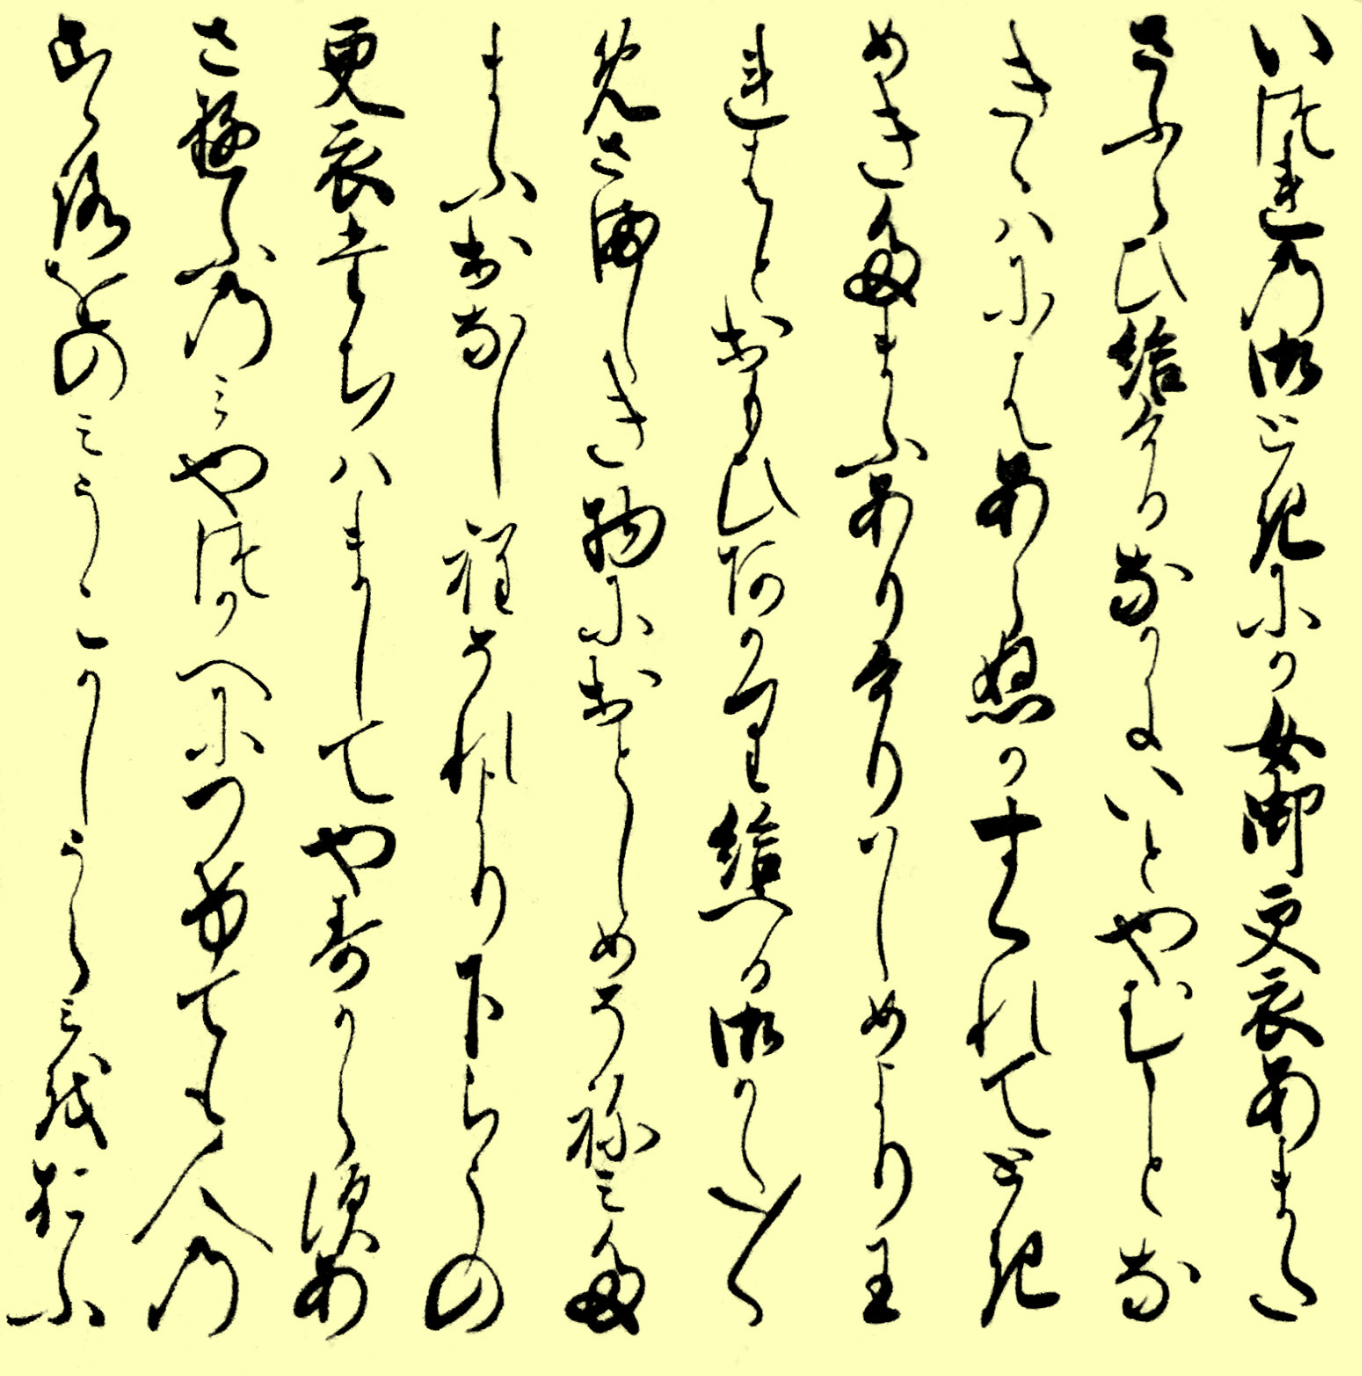
\includegraphics[width=0.55\textwidth]{\GRAPHPATH/genji1}\\
  {\tiny (\citealt{Rickmeyer1991}; 源氏物語:きりつぼ, ca. 1000 u.\,Zr., Manuskript ca.\ 1200 u.\,Zr.}
\end{frame}

\begin{frame}
  {Scriptio continua: Genji no Monogatari}
  \centering
  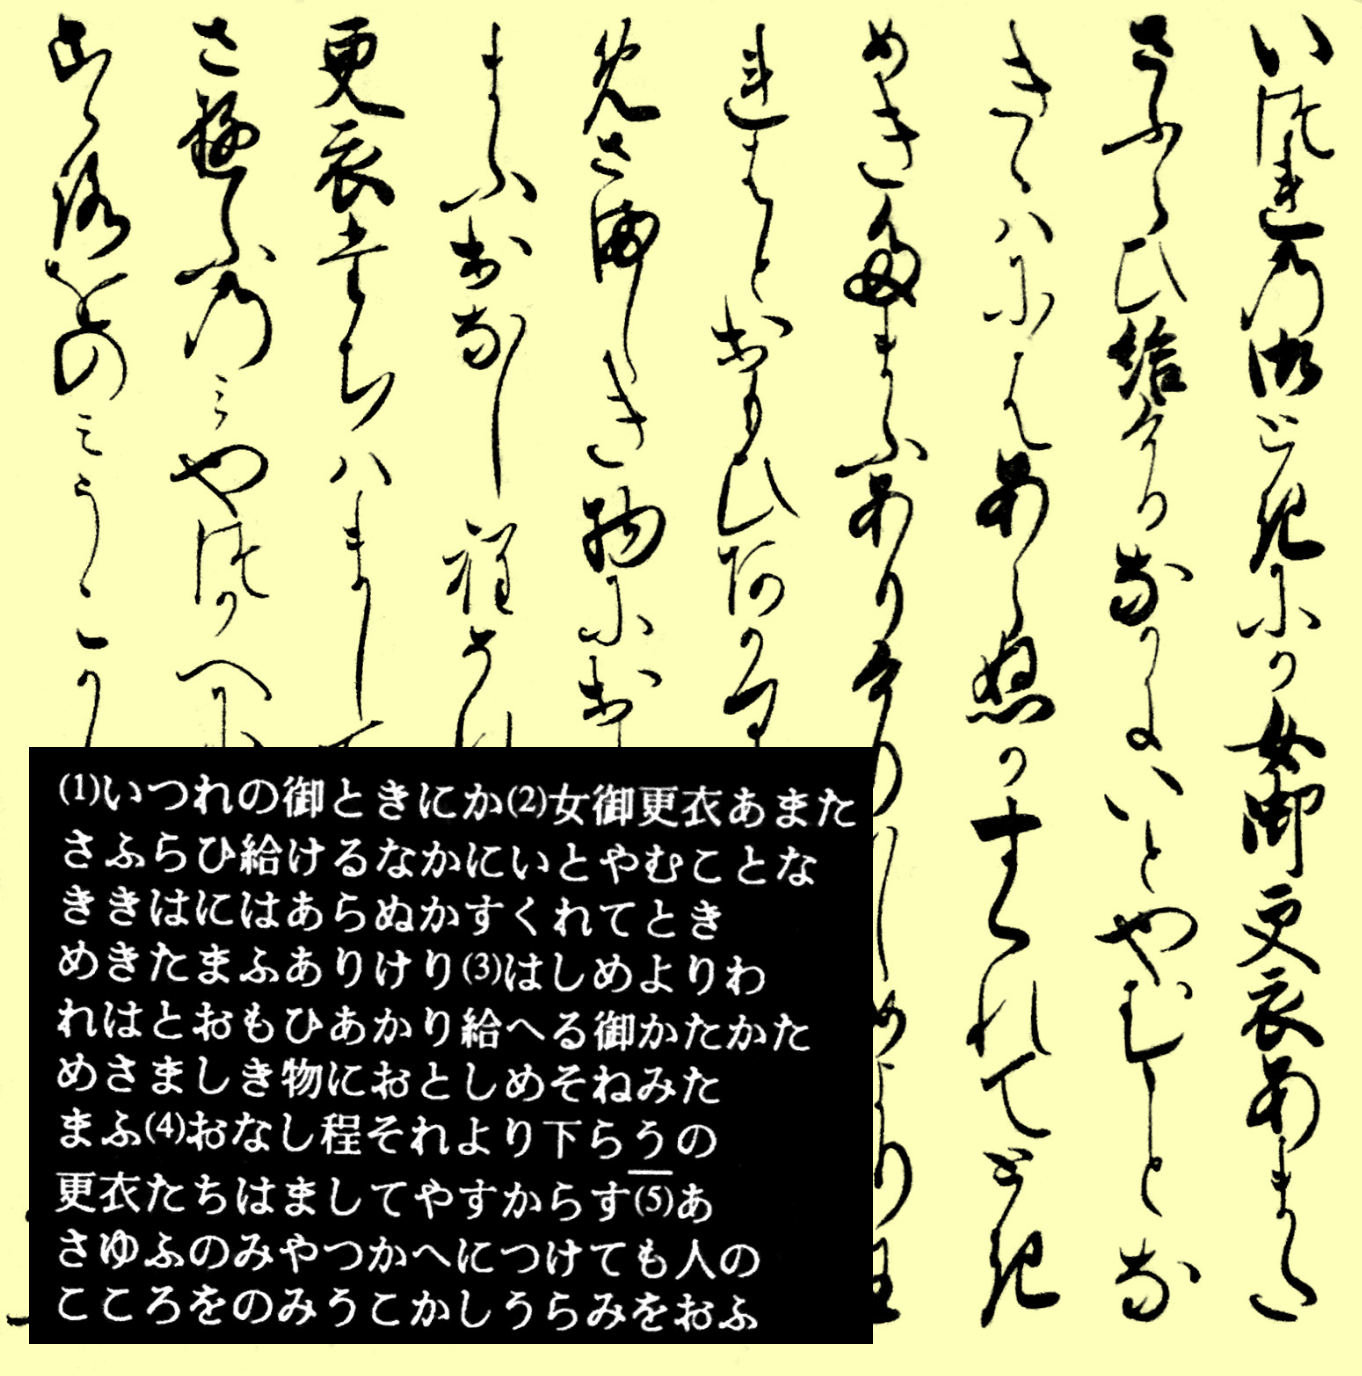
\includegraphics[width=0.55\textwidth]{\GRAPHPATH/genji3}\\
  {\tiny (\citealt{Rickmeyer1991}; 源氏物語:きりつぼ, ca. 1000 u.\,Zr., Manuskript ca.\ 1200 u.\,Zr.}
\end{frame}

\begin{frame}
  {Wie selbstverständlich ist unsere Schreibung?}
  \pause
  \centering
  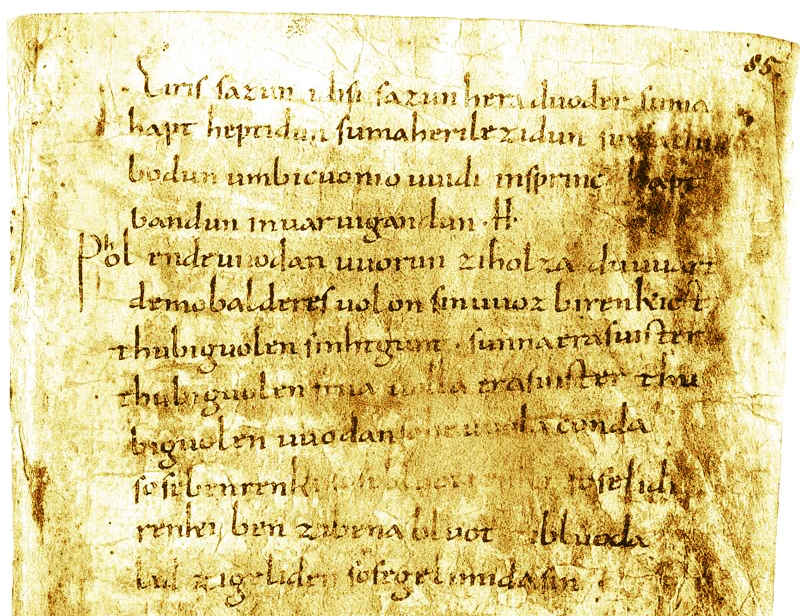
\includegraphics[width=0.8\textwidth]{\GRAPHPATH/merseburg}\\[0.5\baselineskip]
  {\tiny 1.~und 2.~Merseburger Zauberspruch, 9.~Jh.\ u.\,Zr., Cod.\ 136, Folio 85r, Domstiftsbibliothek Merseburg (Wikimedia)\\[-1\baselineskip]
    Hintergründe und generelle Einführung in historische Graphematik in \citet{Elmentaler2018}.}
\end{frame}

\begin{frame}
  {Spatien}
  \pause
  \begin{itemize}[<+->]
    \item im Ahd.\ häufig Reste von Scriptio continua
    \item syntaktische Wörter nicht immer getrennt
    \item \alert{Spatienschreibung}: Trennung syntaktischer Wörter
  \end{itemize}
  \pause
  \Halbzeile
  \begin{exe}
    \ex
    \begin{xlist}
      \ex[*]{Vanessa \rot{istgeritten}.}
      \pause
      \ex[*]{Vanessa reitet \rot{indenwald}.}
    \end{xlist}
    \pause
    \Halbzeile
    \ex
    \begin{xlist}
      \ex[*]{Vanessa hat \rot{Gelegen heit}, die \rot{Schreib ung} von Wörtern und Sätzen \rot{gründ lich} zu \rot{unter suchen}.}
      \pause
      \ex[*]{Oma \rot{koch t} der \rot{ausgekühlt en} Vanessa \rot{ein en heiß en} Tee.}
    \end{xlist}
  \end{exe}
  \pause
  \begin{itemize}[<+->]
    \item Eislaufen, Bergsteigen, Mutmachen, Teetrinken (?)
    \item weichklopfen, schlechtreden (?)
    \item nichtöffentlich, nichtprivat (?)
    \item zulasten (?)
  \end{itemize}
\end{frame}

\section[PUMS vs.\ PAMS]{Positionsunabhängige Majuskelschreibung}

\begin{frame}
  {Majuskelschreibungen}
  \pause
  \begin{itemize}[<+->]
    \item \alert{positionsabhängig}: Satzanfang (Syntax)
      \Halbzeile
    \item \alert{positionsunabhängig}: Substantive (Morphologie\slash Lexik)
    \item Positionsunabhängige Majuskelschreibung (PUMS)
      \Halbzeile
    \item Bredel: "`NP-Kopf-Großschreibung"' (= positions\rot{abhängig}, PAMS)
      \begin{itemize}[<+->]
        \item nein, weil auch in Listen, Überschriften usw.
        \item außerdem: dann Annahme SubstP als verschieden von PronP!\\
          \grau{Oder werden Pronomina als NP-Köpfe großgeschrieben?}
        \item jede Rettungsargumentation des PAMS-Ansatzes wird zirkulär 
        \item \ldots\ oder \alert{motiviert} die PUMS statt sie zu beschreiben
        \item \grau{Siehe Schäfer \& Sayatz (in Vorb.).}
      \end{itemize}
  \end{itemize}
\end{frame}


\begin{frame}
  {Propblemfälle für PUMS}
  \pause
  \begin{exe}
    \ex
    \begin{xlist}
      \ex{An der Nacht auf dem Land schätze ich vor allem \alert{das Dunkle}.}
      \pause
      \ex{Alle Pferde müssen geputzt werden. Vanessa putzt \alert{das schwarze}.}
      \pause
      \ex{Vanessa trägt in der Oper \alert{das Schwarze}.}
    \end{xlist}
    \Viertelzeile
    \pause
    \ex
    \begin{xlist}
      \ex[ ]{im \alert{übrigen}}
      \pause
      \ex[*]{im literarischen \rot{Übrigen}}
      \pause
      \ex[*]{Im \rot{Übrigen}\slash In dem \rot{Übrigen}, von dem wir gestern schon gesprochen haben, ist dieses Buch langweilig.}
    \end{xlist}
    \pause
    \Viertelzeile
    \ex
    \begin{xlist}
      \ex[*]{Edgar gab dem Kunden fachmännisches Recht.}
      \pause
      \ex[*]{Edgar setzte den Cadillac in einwandfreien Stand.}
    \end{xlist}
  \end{exe}
  \pause
  \begin{itemize}[<+->]
    \item Konversion
    \item Ellipse
    \item Ellipse plus Lexikalisierung
  \end{itemize}
\end{frame}

% \section{Univerbierung von N+V}
% 
% \newcommand{\exhl}[1]{\alert{#1}}
% 
% \begin{frame}
%   {Grenzfall für Spatien und PUMS}
%   Was würden Sie machen?\\
%   \Zeile
%   \begin{exe}
%   \ex\label{ex:introexamples1}
%   \begin{xlist}
%     \ex Yael weiß, dass Remy \exhl{Rad} \exhl{fährt}.
%     \ex Yael weiß, dass Remy \exhl{radfährt}.
%   \end{xlist}
%   \Zeile
%   \ex
%   \begin{xlist}
%     \ex Yael weiß, dass Remy \exhl{Eis} \exhl{läuft}.
%     \ex Yael weiß, dass Remy \exhl{eisläuft}.
%   \end{xlist}
% \end{exe}
% \end{frame}
% 
% \begin{frame}
%   {Syntaktische Kontexte | Getrenntschreibung}
%   Was kann man auseinander schreiben?\\
%   \Zeile
%   \begin{exe}
%   \ex
%   \begin{xlist}
%     \ex[ ]{Remy \exhl{fährt} gerade \exhl{Rad}.}
%     \ex[ ]{Remy ist gestern \exhl{Rad} \exhl{gefahren}.}
%     \Zeile
%     \ex[ ]{Remy hat keine Lust, \exhl{Rad} \exhl{zu} \exhl{fahren}.}
%     \ex[ ]{Yael weiß, dass Remy \exhl{Rad} \exhl{fährt}.}
%     \ex[ ]{Remy will \exhl{Rad} \exhl{fahren}.}
%     \Zeile
%     \ex[ ]{Remy ist am \exhl{Rad} \exhl{fahren}.}
%     \Zeile
%     \ex[ ]{Remy singt beim \exhl{Rad} \exhl{fahren}.}
%     \ex[*]{Remy lobt das \exhl{Rad} \exhl{fahren}.}
%     \end{xlist}
%   \end{exe}
% \end{frame}
% 
% \begin{frame}
%   {Syntaktische Kontexte | Zusammenschreibung}
%   \begin{exe}
%   \ex
%   \begin{xlist}
%     \setcounter{xnumii}{1}
%     \ex[ ]{Remy ist gestern \exhl{radgefahren}.}
%     \ex[ ]{Remy hat keine Lust, \exhl{radzufahren}.}
%     \ex[ ]{Yael weiß, dass Remy \exhl{radfährt}.}
%     \ex[ ]{Remy will \exhl{radfahren}.}
%     \ex[ ]{Remy ist am \exhl{Radfahren\slash radfahren}.}
%     \ex[ ]{Remy singt beim \exhl{Radfahren\slash radfahren}.}
%     \ex[ ]{Remy lobt das \exhl{Radfahren}.}
%   \end{xlist}
% \end{exe}
% \end{frame}
% 
% 
% \begin{frame}
%   {Mögliche Einflussfaktoren}
%   \begin{itemize}[<+->]
%     \item (morpho-)syntaktischer \alert{Kontext}
%       \begin{itemize}[<+->]
%         \item Infinitiv
%         \item Partizip
%         \item \textit{am}-Progressiv
%         \item NP (in Präposition)
%       \end{itemize}
%       \Zeile
%     \item \alert{semantische Relation} zwischen N und V
%       \begin{itemize}[<+->]
%         \item Argument
%         \item oblique
%         \item unbestimmbar
%       \end{itemize}
%       \Zeile
%     \item individuelle \alert{Lexikalisierungstendenz}\\
%       \grau{stärkere Bildung eines neuen komplexen semantischen Konzepts}
%   \end{itemize}
% \end{frame}
% 
% \begin{frame}
%   {Schäfer \& Sayatz (eingereicht)}
%   \centering 
%   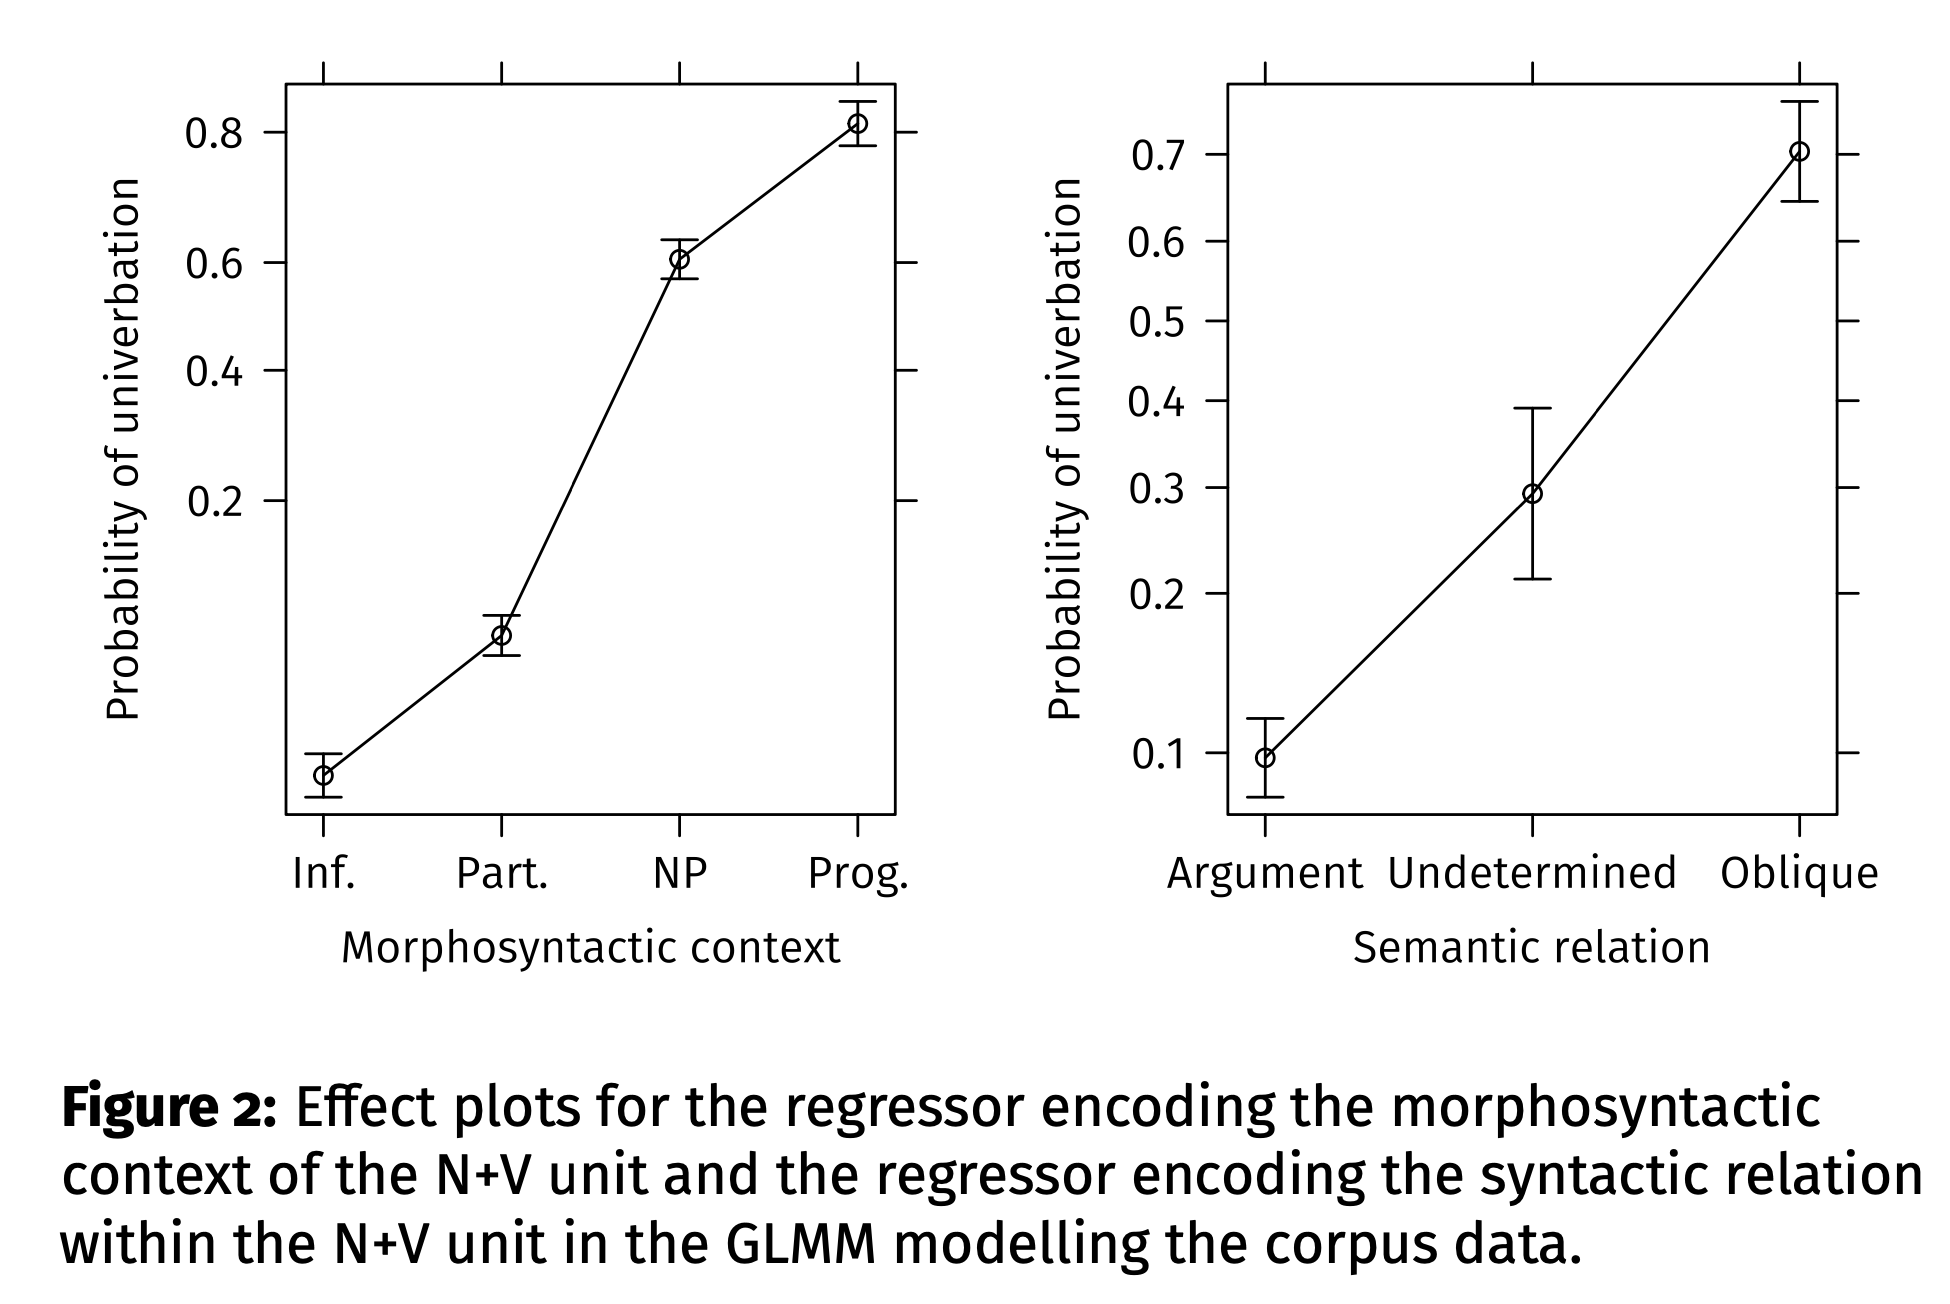
\includegraphics[width=0.7\textwidth]{\GRAPHPATH/nv2}
% \end{frame}
% 
% \begin{frame}
%   {Schäfer \& Sayatz (eingereicht)}
%   \centering 
%   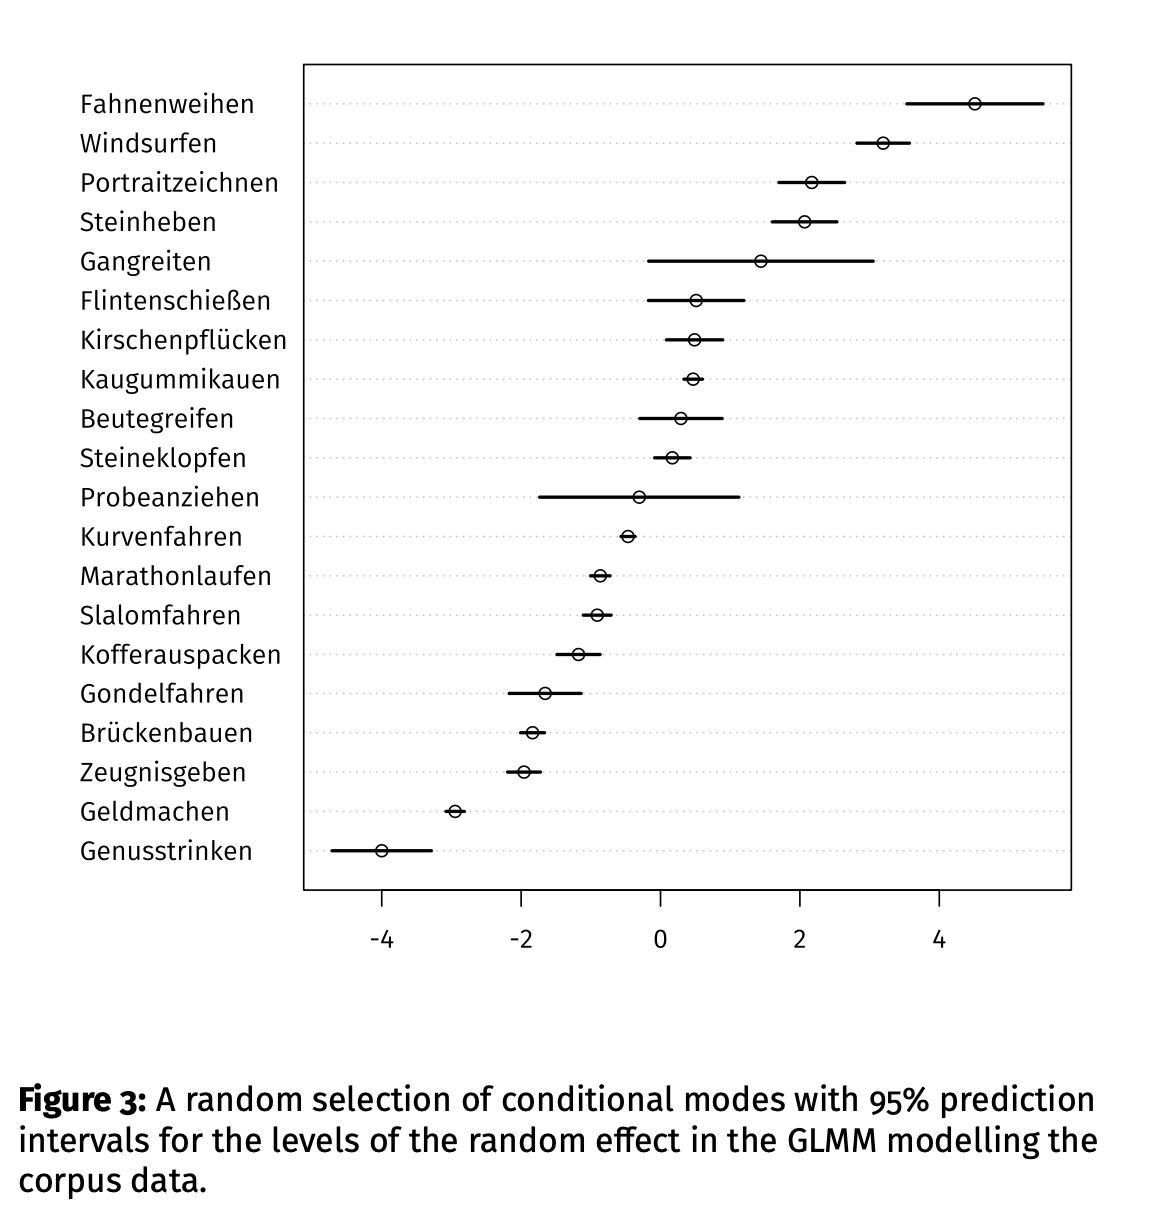
\includegraphics[width=0.7\textwidth]{\GRAPHPATH/nv3}
% \end{frame}
% 
% \begin{frame}
%   {Schäfer \& Sayatz (eingereicht)}
%   \centering 
%   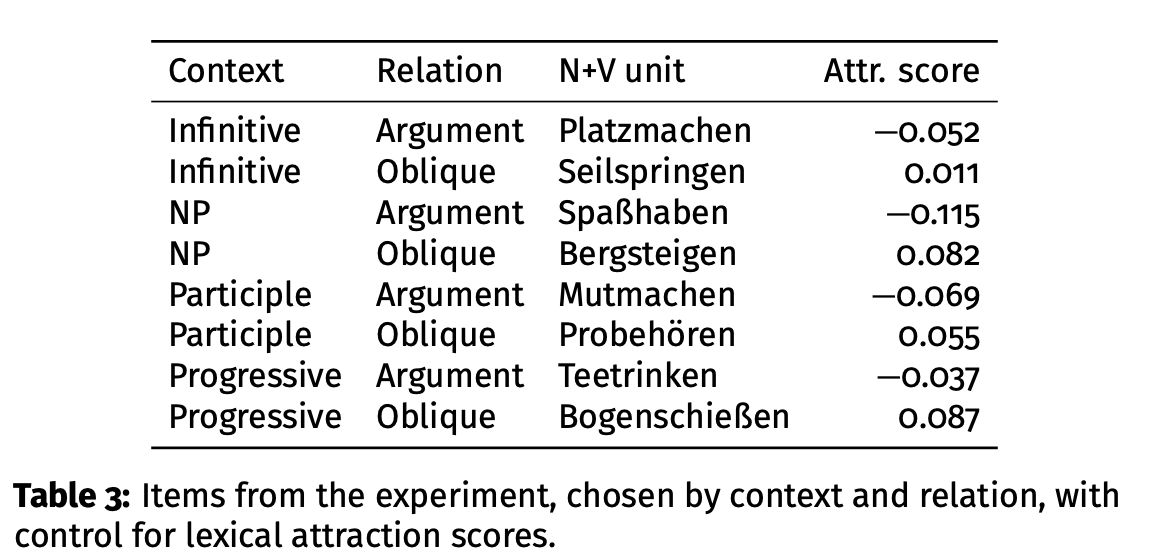
\includegraphics[width=0.7\textwidth]{\GRAPHPATH/nv4}
% \end{frame}
% 
% \begin{frame}
%   {Schäfer \& Sayatz (eingereicht)}
%   \centering 
%   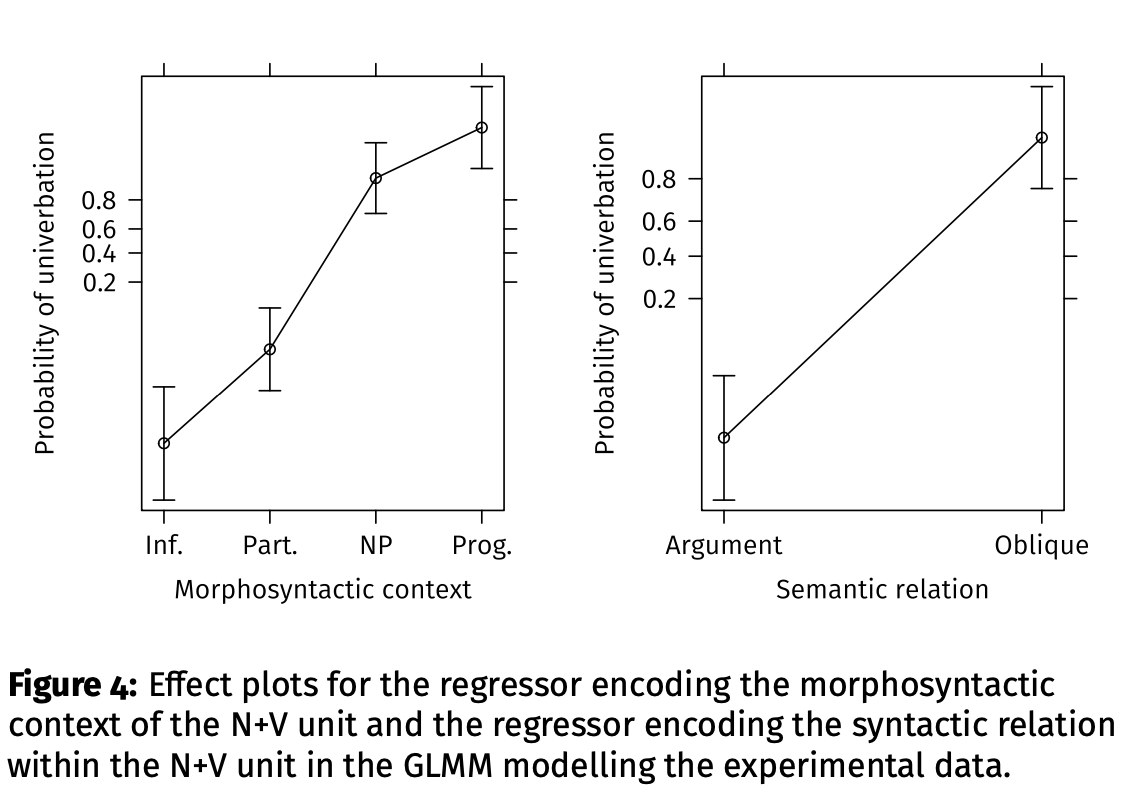
\includegraphics[width=0.7\textwidth]{\GRAPHPATH/nv5}
% \end{frame}
% 
% \begin{frame}
%   {Schäfer \& Sayatz (eingereicht)}
%   \centering 
%   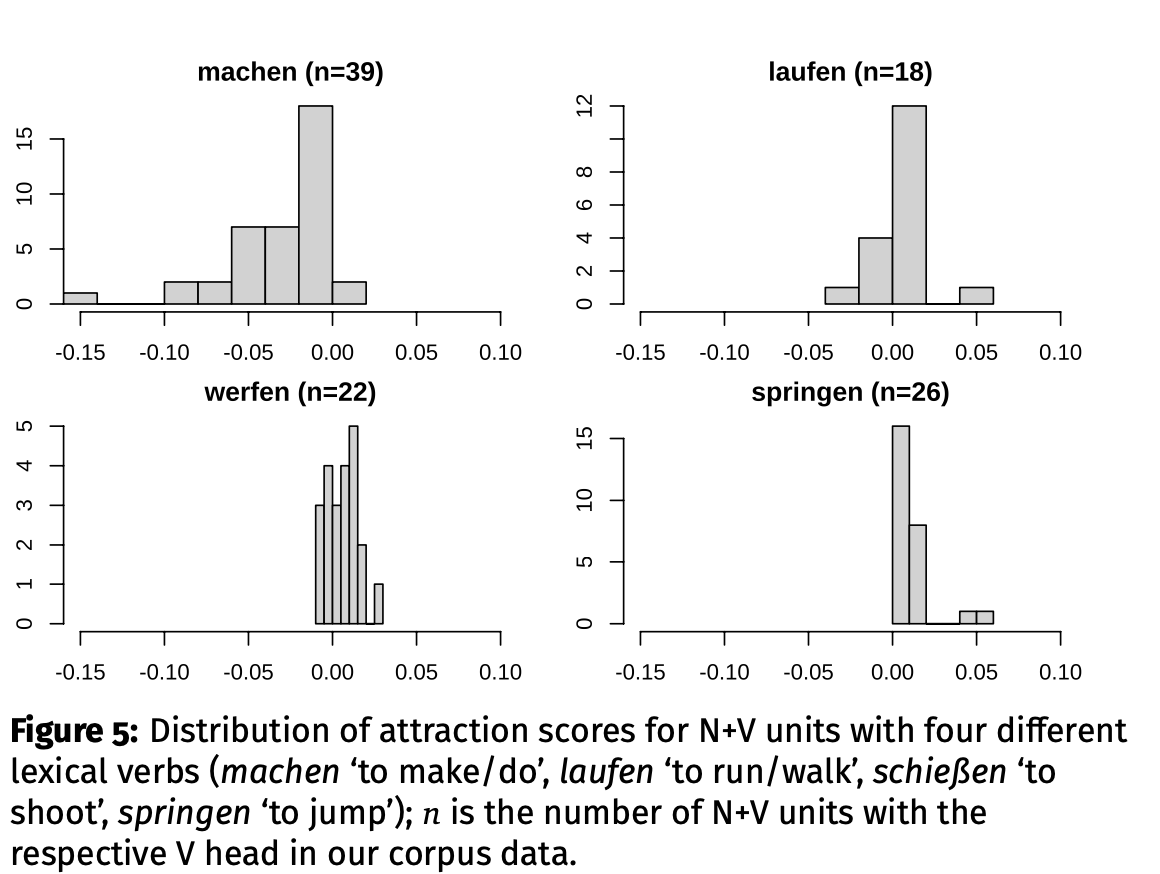
\includegraphics[width=0.7\textwidth]{\GRAPHPATH/nv6}
% \end{frame}
% 
% \begin{frame}
%   {Grundsätzliche theroretische Erkenntnis}
%   Gebrauchsbasierte Graphematik\\
%   \Zeile
%   \begin{itemize}[<+->]
%     \item Lernen von Generalisierungen über Ähnlichkeiten
%     \item konfligierende Beschränkungen\slash Einflussfaktoren
%     \item nicht immer harte Trennung | \alert{probabilistische Grammatik}
%       \Zeile
%     \item arbiträre Normierung
%     \item klarer Fall für permissive Normierung
%   \end{itemize}
% \end{frame}


\ifdefined\TITLE
  \section{Nächste Woche | Überblick}

  \begin{frame}
    {Semesterplan}
    \begin{enumerate}
      \item Graphematik und Schreibprinzipien
      \item Wiederholung -- Phonetik
      \item Wiederholung -- Phonologie
      \item Phonographisches Schreibprinzip -- Konsonanten
      \item Phonographisches Schreibprinzip -- Vokale
      \item Silben und Dehnungsschreibungen
      \item Eszett, Dehnung und Konstanz
      \item Spatien und Majuskeln
      \item \alert{Komma}
      \item Punkt und sonstige Interpunktion
    \end{enumerate}
  \end{frame}
\fi


  \let\subsection\section\let\section\woopsi
  
  \section{09. Komma}
  \let\woopsi\section\let\section\subsection\let\subsection\subsubsection
  \section{Übersicht}

\begin{frame}
  {Übersicht}
  \onslide<+->
  \begin{itemize}[<+->]
    \item Wo stehen Kommata?
      \Zeile
    \item Doppelfunktion oder Monofunktion?
    \item Probleme
      \Zeile
    \item Empirie | \textit{obwohl} und \textit{weil} mit V2
  \end{itemize}
\end{frame}

\section[Befund]{Deskriptiver Befund}

\begin{frame}
  {Aufzählung}
  \onslide<+->
  \onslide<+->
  \begin{exe}
    \ex \alert{Peter, Paul und Mary} gehen in den Zoo.
    \ex \alert{Unter, neben und über} dem Werkstück für genügend Freiraum achten.
    \ex \alert{Wandern, Schwimmen, Radfahren} -- Volkssport pur!
    \ex Die Verbindung erfolgt \alert{form-, kraft- oder stoff}schlüssig.
  \end{exe}
  \onslide<+->
  \Zeile
  Kommatierung ist hier so flexibel wie Koordinationsstrukturen eben sind.
\end{frame}

\begin{frame}
  {Sätze}
  \onslide<+->
  \onslide<+->
  \begin{exe}
    \ex
    \begin{xlist}
	  \ex \grau{Die Sonne geht unter, der Mond geht auf.}
	  \ex \grau{Die Sonne geht unter, und der Mond geht auf.}
    \end{xlist}
    \Zeile
    \ex Adrianna weiß, \alert{dass es gleich regnen} \orongsch{wird}.
    \ex Michelle geht, \alert{obwohl die Party erst} \orongsch{beginnt}.
    \ex Adrianne hilft der Kollegin, \alert{die nassgeregnet} \orongsch{wurde}.
    \Zeile
    \ex \tuerkis{Adrianna glaubt, die Regenwolken zu sehen.}
  \end{exe}
  \onslide<+->
  \Zeile
  Diese Satzkommas lassen sich gut auf eine syntaktische Domäne eingrenzen.
\end{frame}

\begin{frame}
  {Sonstiges}
  \onslide<+->
  \onslide<+->
  \begin{exe}
    \ex Adrianna, \alert{eine Kollegin}, wurde nassgeregnet.
    \ex Die, \alert{übrigens unsinnige}, Behauptung der Monofunktion\\
    wird kaum vertreten.
    \ex Michelle will den Dobermann aufnehmen, \alert{als Pflegestelle}.
    \ex \alert{Ja}, Michelle kennt Adrianna.
  \end{exe}
  \onslide<+->
  \Zeile
  Hat das Komma hier primär einen Intonationseffekt?
\end{frame}

\section[Erklärung]{Erklärungsansätze}

\begin{frame}
  {Syntax | Doppelfunktion (Primus usw.)}
  \onslide<+->
  \onslide<+->
  Gibt es überhaupt eine "`Theorie des Kommas"'?\\
  \onslide<+->
  \Zeile
  \begin{itemize}[<+->]
    \item Nein | Ziel: \alert{optimale Beschreibungen von Verteilungen}\\
	    \Zeile
    \item syntaktisch keine Gemeinsamkeit zwischen Koordination und Nebensatz
    \item \ldots\ \alert{aber beides auf jeden Fall rein syntaktisch definierte Grenzen!}
	    \Halbzeile
    \item \alert{Intonationsgrenzen?} --- ja, als Folge der syntaktischen Grenze
    \item aber \rot{viele Intonationsgrenzen ohne Komma}
  \end{itemize}
\end{frame}


\begin{frame}
  {Syntax von Koordination}
  \alert{Verbindung von kategorial Gleichem zu kategorial Gleichem},\\
  kein Kopfstatus | beliebig simplexe oder komplexe Kategorien\\
  \Zeile
  \centering 
  \scalebox{0.8}{%
  \begin{forest}
    [\textbf{N}, calign=child, calign child=2
      [\textbf{N}, tier=preterminal
        [\it Kuchen]
      ]
      [Konj, tier=preterminal
        [{\it \alert{und}\ \slash\ \alert{,}}]
      ]
      [\textbf{N}, tier=preterminal
        [\it Sahne]
      ]
    ]
  \end{forest}}~\hspace{2em}~%
  \scalebox{0.8}{%
  \begin{forest}
    [S, calign=child, calign child=2
      [S, tier=preterminal
        [\it Es ist Sonntag, narroof]
      ]
      [Konj, tier=preterminal
        [{\it {und}\ \slash\ \alert{,}}]
      ]
      [S, tier=preterminal
        [\it die Zeit wird knapp, narroof]
      ]
    ]
  \end{forest}}
\end{frame}

\begin{frame}
  {Syntax von Satzeinbettung (Beispiel)}
  \alert{Strukturen mit (finitem) Verb und allen Abhängigen} |\\
  funktional Ergänzungen, Angaben, Attribute, evtl.\ max.\ eine Spur\\
  \Zeile
  \centering
  \scalebox{0.8}{%
  \begin{forest}
    [NP, calign=child, calign child=2
      [Art, tier=preterminal
        [\it einen]
      ]
      [\bf N, tier=preterminal
        [\it Tofu \alert{,}]
      ]
      [RS, calign=first
        [NP\Sub{1}, tier=preterminal
          [\it der, narroof, name=BeweDer]
        ]
        [VP, calign=last
          [NP, tier=preterminal
            [\it mir, narroof]
          ]
          [\Ti, tier=preterminal]
          {\draw[dotted, thick, ->] (.south) |- ++(0,-4.5em) -| (BeweDer.south);}
          [Ptkl, tier=preterminal
            [nicht]
          ]
          [\bf V, calign=last
            [\bf V, tier=preterminal
              [\it geschmeckt]
            ]
            [\bf V, tier=preterminal
              [\it hat]
            ]
          ]
        ]
      ]
    ]
  \end{forest}}
\end{frame}

\begin{frame}
  {Syntax | Bredels Monofunktion I}
  \onslide<+->
  \begin{itemize}[<+->]
	  \item Behauptung | \alert{Doppelfunktion "`nicht lernbar"'}
		  \Zeile
    \item Wie bitte?
	    \Halbzeile
	    \begin{itemize}[<+->]
		    \item \alert{Homonymie?}\\
			    \textit{Kiefer}, \textit{Schloss}, \textit{Bank}
			    \Halbzeile
		    \item \alert{Synkretismus?}\\
			    \textit{dieser}, \textit{Menschen}, \textit{laufen}
			    \Halbzeile
		    \item \alert{strukturelle Ambiguität?}\\
			    \textit{Scully beobachtet den Außerirdischen mit dem Teloskop.}
	    \end{itemize}
  \end{itemize}
\end{frame}

\begin{frame}
  {Syntax | Bredels Monofunktion II}
  \onslide<+->
  \begin{itemize}[<+->]
	  \item Komma markiert \alert{"`Grenze im Parsingprozess"'}
          \item kein normales Weiterparsen wie vorher
	  \item also "`Online-Funktion"' in der Syntaxverarbeitung
		  \Halbzeile
	  \item \rot{keine} zugrundeliegende Syntaxtheorie\\
            \grau{Es gibt formale Theorien inkrementeller Verarbeitung!}
	  \item \rot{keine} ausgearbeitete Verabreitungstheorie
            \Halbzeile
	  \item beliebig \rot{allgemeine Beschreibung} = immer Monofunktion\\
		  \grau{Die Funktion jedes Wortes ist die sprachliche Kommunikation!}
  \end{itemize}
\end{frame}

\begin{frame}
  {Syntax | Bredels Monofunktion III}
  \onslide<+->
  \onslide<+->
  Die (Fremd-)Daten sind nicht falsch, nur die Schlussfolgerung.\\
  \Zeile
  \begin{itemize}[<+->]
	  \item ähnlich wie bei der NP-Kopf-Großschreibung \ldots
            \Halbzeile
		  \begin{itemize}[<+->]
                          \item \alert{natürlich} markiert Komma irgendwelche Phrasengrenzen
			  \item \alert{natürlich} beim Parsen (Verarbeitung) wichtiges Indiz
				  \Halbzeile
			  \item \grau{Das steht bei den Psycholinguisten, die Bredel rezipiert.}
				  \Halbzeile
			  \item \rot{Aber das erklärt nicht die Verteilung von Kommata im Deutschen!}
		  \end{itemize}
  \end{itemize}
\end{frame}

\begin{frame}
  {Probleme | Satzverbindungen}
  \onslide<+->
  \onslide<+->
  "`Vor \textit{und} steht kein Komma."'\\
  \Zeile
  \onslide<+->
  \begin{exe}
    \ex[ ]{Die Sonne geht unter\alert{,} der Mond geht auf.}
    \ex[ ]{Die Sonne geht unter\alert{, und} der Mond geht auf.}
    \ex[?]{Die Sonne geht unter\rot{, und} die Schlacht von Worringen fand 1288 statt.}
  \end{exe}
  \Zeile
  \begin{itemize}[<+->]
    \item Konflikt | Aufzählungskomma (nie mit \textit{und}) und Satzkomma
    \item Bedingung für Satzkomma stärker \ding{220} \rot{kein Aufzählungskomma}
    \item außerdem spezielle semantische\slash pragmatische Bedingungen\\
      für Verknüpfung, also keine einfache Aufzählung
  \end{itemize}
\end{frame}

\begin{frame}
  {Probleme | Adversative Koordinationspartikeln}
  \onslide<+->
  \onslide<+->
  Warum steht hier ein Komma?\\
  \onslide<+->
  \Zeile
  \begin{exe}
    \ex
    \begin{xlist}
      \ex Wir fahren ein blaues \alert{und} elegantes Auto.
      \ex In der Küche \alert{und} in der Kammer stehen Wäschekörbe.
    \end{xlist}
    \ex
    \begin{xlist}
      \ex Wir fahren ein blaues\rot{, aber} elegantes Auto.
      \ex Nicht in der Küche\rot{, sondern} in der Kammer steht der Wäschekorb.
    \end{xlist}
  \end{exe}
  \Zeile
  \begin{itemize}[<+->]
    \item meines Erachtens nicht systemkonform
    \item \rot{semantisch\slash pragmatisch} motivierte Regel
    \item atypisch für das Deutsche
  \end{itemize}
\end{frame}

\begin{frame}
	{Probleme | Vorfeldkomma}
	\begin{exe}
		\ex[+]{\rot{Die erfolgreiche Gewichtheberin,} gewann die EM.}
		\ex[+]{\rot{In der Regel,} werden für Reißen und Stoßen\\
	gesonderte Medaillen vergeben.}
		\ex[+]{\rot{Außer bei Olympischen Spielen,} werden für Reißen und Stoßen gesonderte Medaillen vergeben.}
	\end{exe}
	\Zeile
	\onslide<+->
	\begin{itemize}[<+->]
		\item typischerweise bei Adverbialen im Vorfeld (Berg 2020)
		\item und eine gewisse Abhängigkeit von der Vorfeld-Länge
			\Halbzeile
		\item hochrelevant | \alert{weder nach Mono- oder Polyfunktionsanalyse erwartbar}
		\item kognitiv unbekannte Kategorisierung des Kommas bei Sprechern
	\end{itemize}
\end{frame}

\begin{frame}
  {Probleme | \textit{Infinitvkonstruktionen}}
  \begin{exe}
    \ex[*]{Nadezhda \rot{scheint}, die Kontrolle über die Hantel zu verlieren.}
    \ex[*]{Nadezhda \rot{will}, die Weltmeisterschaft gewinnen.}
    \ex[ ]{Nadezhda \alert{beschließt}, keine Steroide mehr einzunehmen.}
    \ex[?]{Nadezhda \alert{beschließt}\orongsch{,} zu trainieren.}
  \end{exe}
  \onslide<+->
  \Zeile
  \begin{itemize}[<+->]
    \item \alert{Infinitivsyntax} ist der Schlüssel
    \item Komma nur bei \alert{inkohärenten Infinitiven}
  \end{itemize}
\end{frame}

\begin{frame}
  {Probleme | Inkohärente Infinitive}
  Kohärente und inkohärente Infinitivkonstruktionen\\
  \onslide<+->
  \Zeile
  \centering
  \scalebox{0.7}{%
  \begin{forest}
    [VP\Sub{1+2}, calign=last
      [NP, tier=preterminal
        [\textit{Vanessa}, narroof]
      ]
      [NP, tier=preterminal
        [\textit{die Pferde}, narroof]
      ]
      [\textbf{V\Sub{2+1}}, calign=last
        [\textbf{V\Sub{2}}, tier=preterminal
          [\textit{behufen}]
        ]
        [\textbf{V\Sub{1}}, tier=preterminal
          [\textit{will}]
        ]
      ]
    ]
  \end{forest}}~\hspace{2em}~%
  \scalebox{0.7}{%
  \begin{forest}
    l sep+=3em, s sep+=2em
    [VP\Sub{1}, calign=last
      [NP, tier=preterminal
        [\textit{Vanessa}, narroof]
      ]
      [VP\Sub{2}, calign=last
        [NP, tier=preterminal
          [\textit{die Pferde}, narroof]
        ]
        [\textbf{V\Sub{2}}, tier=preterminal
          [\textit{zu behufen}]
        ]
      ]
      [\textbf{V\Sub{1}}, tier=preterminal
        [\textit{wünscht}]
      ]
    ]
  \end{forest}}
\end{frame}


\begin{frame}
  {Probleme | (In)kohärente Infinitve}
  \onslide<+->
  \onslide<+->
    \resizebox{1\textwidth}{!}{
    \begin{tabular}{lcllll}
      \lsptoprule
      & \multirow{2}{*}{\textbf{Status}} & \multirow{2}{*}{\textbf{Kohärenz}} & \textbf{eigenes} & \textbf{Subjekts-} \\
      & & & \textbf{Subjekt} & \textbf{Rolle} & \textbf{Beispiel}\\
      \midrule
      \textbf{Modalverben} & 1 & obl.\ kohärent & ja & Identität & \textit{wollen} \\
      \textbf{Halbmodalverben} & 2 & obl.\ kohärent & nein & nein & \textit{scheinen} \\
      \textbf{Kontrollverben} & 2 & \rot{opt.\ inkohärent} & ja & Kontrolle & \textit{beschließen} \\
      \lspbottomrule
    \end{tabular}
  }\\
  \Zeile
  \begin{itemize}[<+->]
    \item Nur \alert{inkohärente nachgestellte Infinitive} werden kommatiert!
    \item Sie gelten als satzwertig, aber die \rot{Inkohärenz ist leider nur optional}.
    \item Es kommen also nur \alert{Abhängige von Kontrollverben} infrage.
  \end{itemize}
  \onslide<+->
  \Viertelzeile
  \begin{exe}
    \ex[*]{Nadezhda \rot{scheint}, die Kontrolle über die Hantel zu verlieren.}
    \ex[*]{Nadezhda \rot{will}, die Weltmeisterschaft gewinnen.}
  \end{exe}
\end{frame}

\begin{frame}
  {Probleme | (In)kohärente Infinitve}
  \onslide<+->
  \onslide<+->
  Was ist jetzt hiermit?\\
  \Halbzeile
  \onslide<+->
  \begin{exe}
    \ex[ ]{Nadezhda \alert{beschließt}, keine Steroide mehr einzunehmen.}
    \ex[?]{Nadezhda \alert{beschließt}\orongsch{,} zu trainieren.}
  \end{exe}
  \onslide<+->
  \Halbzeile
  \alert{Eindeutig inkohärent} | hinter die RSK versetzte Infinitive\\
  \Viertelzeile
  \onslide<+->
  \begin{exe}
    \ex \rot{\textbf{Inkohärent}}
    \begin{xlist}
      \ex[ ]{\ldots dass Nadezhda beschließt, keine Steroide mehr zu nehmen.}
      \ex[?]{\ldots dass Nadezhda keine Steroide mehr zu nehmen beschließt.}
    \end{xlist}
    \ex \alert{\textbf{Kohärent oder inkohärent}}
    \begin{xlist}
      \ex[ ]{\ldots dass Nadezhda zu trainieren beschließt.}
      \ex[ ]{\ldots dass Nadezhda beschließt zu trainieren.}
    \end{xlist}
  \end{exe}
\end{frame}


\begin{frame}
  {Probleme | (In)kohärente Infinitve}
  Es liegt also an der syntaktischen Struktur.\\
  \Zeile
  \onslide<+->
  \begin{exe}
    \ex
    \begin{xlist}
      \ex[ ]{[Nadezhda]\Sub{2} \alert{[beschließt]\Sub{1}} [[t\Sub{2} \gruen{t\Sub{3}} \alert{[t\Sub{1}]\Sub{VK}}]\ \Sub{VP}\ \orongsch{,}\\
      {\hspace{1em}}\gruen{[keine Steroide mehr einzunehmen]\Sub{3}}]\Sub{VP}.}
        \Viertelzeile
      \ex[*]{[Nadezhda]\Sub{2} \rot{[beschließt]\Sub{1}}\\
      {\hspace{1em}}[t\Sub{2} [keine Steroide] [mehr] \rot{[einzunehmen t\Sub{1}]\Sub{VK}}\ ]\Sub{VP}.\label{ex:ohweia}}
    \end{xlist}
    \Halbzeile
    \ex
    \begin{xlist}
      \ex[ ]{[Nadezhda]\Sub{2} \alert{[beschließt]\Sub{1}}\ \orongsch{,} [[t\Sub{2} \gruen{t\Sub{3}} \alert{[t\Sub{1}]\Sub{VK}}\ ]\Sub{VP} \gruen{[zu trainieren]\Sub{3}}]\Sub{VP}.}
      \Viertelzeile
      \ex[ ]{[Nadezhda]\Sub{2} \tuerkis{[beschließt]\Sub{1}} [t\Sub{2} \tuerkis{[zu trainieren t\Sub{1}]\Sub{VK}}\ ]\Sub{VP}}
    \end{xlist}
  \end{exe}
  \Halbzeile
  \onslide<+->
  Füllen Sie den VK durch Hinzufügen von Hilfsverben auf,\\
  um das Phänomen noch deutlicher zu sehen.
\end{frame}

\begin{frame}
  {Probleme | Bäume für inkohärente Konstruktion}
  \onslide<+->
  \onslide<+->
  \rot{Inkohärent konstruiert}\\
  \Zeile
  \centering 
  \begin{forest}
    [S, calign=child, calign child=2
      [NP\Sub{2}, tier=pt
        [\it Nadezhda, narroof, tier=t]
      ]
      [V\Sub{1}, tier=pt
        [\it beschließt, tier=t]
      ]
      [VP, calign=child, calign child=1
        [VP, calign=child, calign child=3
          [\Tii, tier=t]
          [\rot{\Tiii}, tier=t]
          [\Ti, tier=t]
        ]
        [VP\Sub{3}, tier=pt, rottree
          [\it keine Steroide mehr einzunehmen, narroof, tier=t]
        ]
      ]
    ]
  \end{forest}
\end{frame}


\begin{frame}
  {Probleme | Bäume für inkohärente Konstruktion mit Hilfsverb}
  \onslide<+->
  \onslide<+->
  Dank des Verbs im Verbkomplex \rot{sieht man die Extraktion}\\
  \Zeile
  \centering 
  \begin{forest}
    [S, calign=child, calign child=2
      [NP\Sub{2}, tier=pt, tier=pt
        [\it Nadezhda, tier=t, narroof]
      ]
      [V\Sub{1}, tier=pt
        [\it hat, tier=t]
      ]
      [VP, , calign=child, calign child=1
        [VP, calign=last
          [\Tii, tier=t, forky]
          [\rot{\Tiii}, tier=t, forky]
          [V, calign=last
            [V, tier=pt
              [\it beschlossen, tier=t]
            ]
            [\Ti, tier=t]
          ]
        ]
        [VP\Sub{3}, tier=pt, rottree
          [\it keine Steroide mehr einzunehmen, narroof, tier=t]
        ]
      ]
    ]
  \end{forest}
\end{frame}


\begin{frame}
  {Probleme | Bäume für kohärente Konstruktion mit Hilfsverb}
  \onslide<+->
  \onslide<+->
  \rot{So gut wie ungrammatisch!}\\
  \Zeile
  \centering 
  \begin{forest}
    [S, calign=child, calign child=2
      [NP\Sub{2}, tier=pt
        [\it Nadezhda, tier=t, narroof]
      ]
      [V\Sub{1}, tier=pt
        [\it hat, tier=t]
      ]
      [VP, calign=last
        [\Tii, tier=t, forky]
        [NP, tier=pt
          [\it keine Steroide, narroof, tier=t]
        ]
        [AdvP, tier=pt
          [\it mehr, narroof, tier=t]
        ]
        [V, calign=last
          [V, calign=last
            [V
              [\it einzunehmen]
            ]
            [V, tier=pt
              [\it beschlossen, tier=t]
            ]
          ]
          [\Ti, tier=t]
        ]
      ]
    ]
  \end{forest}
\end{frame}

\begin{frame}
  {Probleme | Bäume für kohärente Konstruktion ohne Hilfsverb}
  \onslide<+->
  \onslide<+->
  Man kann daher davon ausgehen, dass diese Struktur auch nicht grammatisch ist.\\
  \onslide<+->
  \Viertelzeile
  Sie entspricht (\ref{ex:ohweia}), also der nicht kommatierten Version.\\
  \onslide<+->
  \Zeile
  \centering
  \begin{forest}
    [S, calign=child, calign child=2
      [NP\Sub{2}, tier=pt
        [\it Nadezhda, tier=t, narroof]
      ]
      [V\Sub{1}, tier=pt
        [\it beschließt, tier=t]
      ]
      [VP, calign=last
        [\Tii, tier=t, forky]
        [VP\Sub{3}, tier=pt, rottree
          [\it keine Steroide, narroof, tier=t]
        ]
        [AdvP, tier=pt
          [\it mehr, narroof]
        ]
        [V, calign=last
          [V, tier=pt
            [\it einzunehmen]
          ]
          [\Ti, tier=t]
        ]
      ]
    ]
  \end{forest}
\end{frame}


\begin{frame}
  {Probleme | Herausstellungen und Nichtintegration}
  \onslide<+->
  \onslide<+->
  \begin{exe}
    \ex Adrianna, \alert{eine Kollegin}, wurde nassgeregnet.
    \ex Die, \alert{übrigens unsinnige}, Behauptung der Monofunktion\\
    wird kaum vertreten.
    \ex Michelle will den Dobermann aufnehmen, \alert{als Pflegestelle}.
    \ex \alert{Ja}, Michelle kennt Adrianna.
  \end{exe}
  \onslide<+->
  \Halbzeile
  \begin{itemize}[<+->]
    \item \alert{Parenthesen} und \alert{Herausstellungen} im weiteren Sinn
    \item am ehesten Bredels Unterbrechung im Parsing
    \item bzw.\ \alert{Unterbrechung in der syntaktischen Struktur}
    \item die \alert{dritte Kommafunktion}?
      \Halbzeile
    \item Nanna Fuhrhop | "`pränominale Herausstellung ist Bindestrichfunktion"'\\
      \rot{entspricht aber nicht der Realität} (s.\ Sayatz und Schäfer i.\,V.)
  \end{itemize}
\end{frame}


\section[Unabhängigkeit]{Unabhängigkeit von Sätzen | \citet{SchaeferSayatz2016}}


\begin{frame}
  {\textit{obwohl} und \textit{weil} mit V2}
  \citet{SchaeferSayatz2016}\\
  \Zeile
  \centering 
  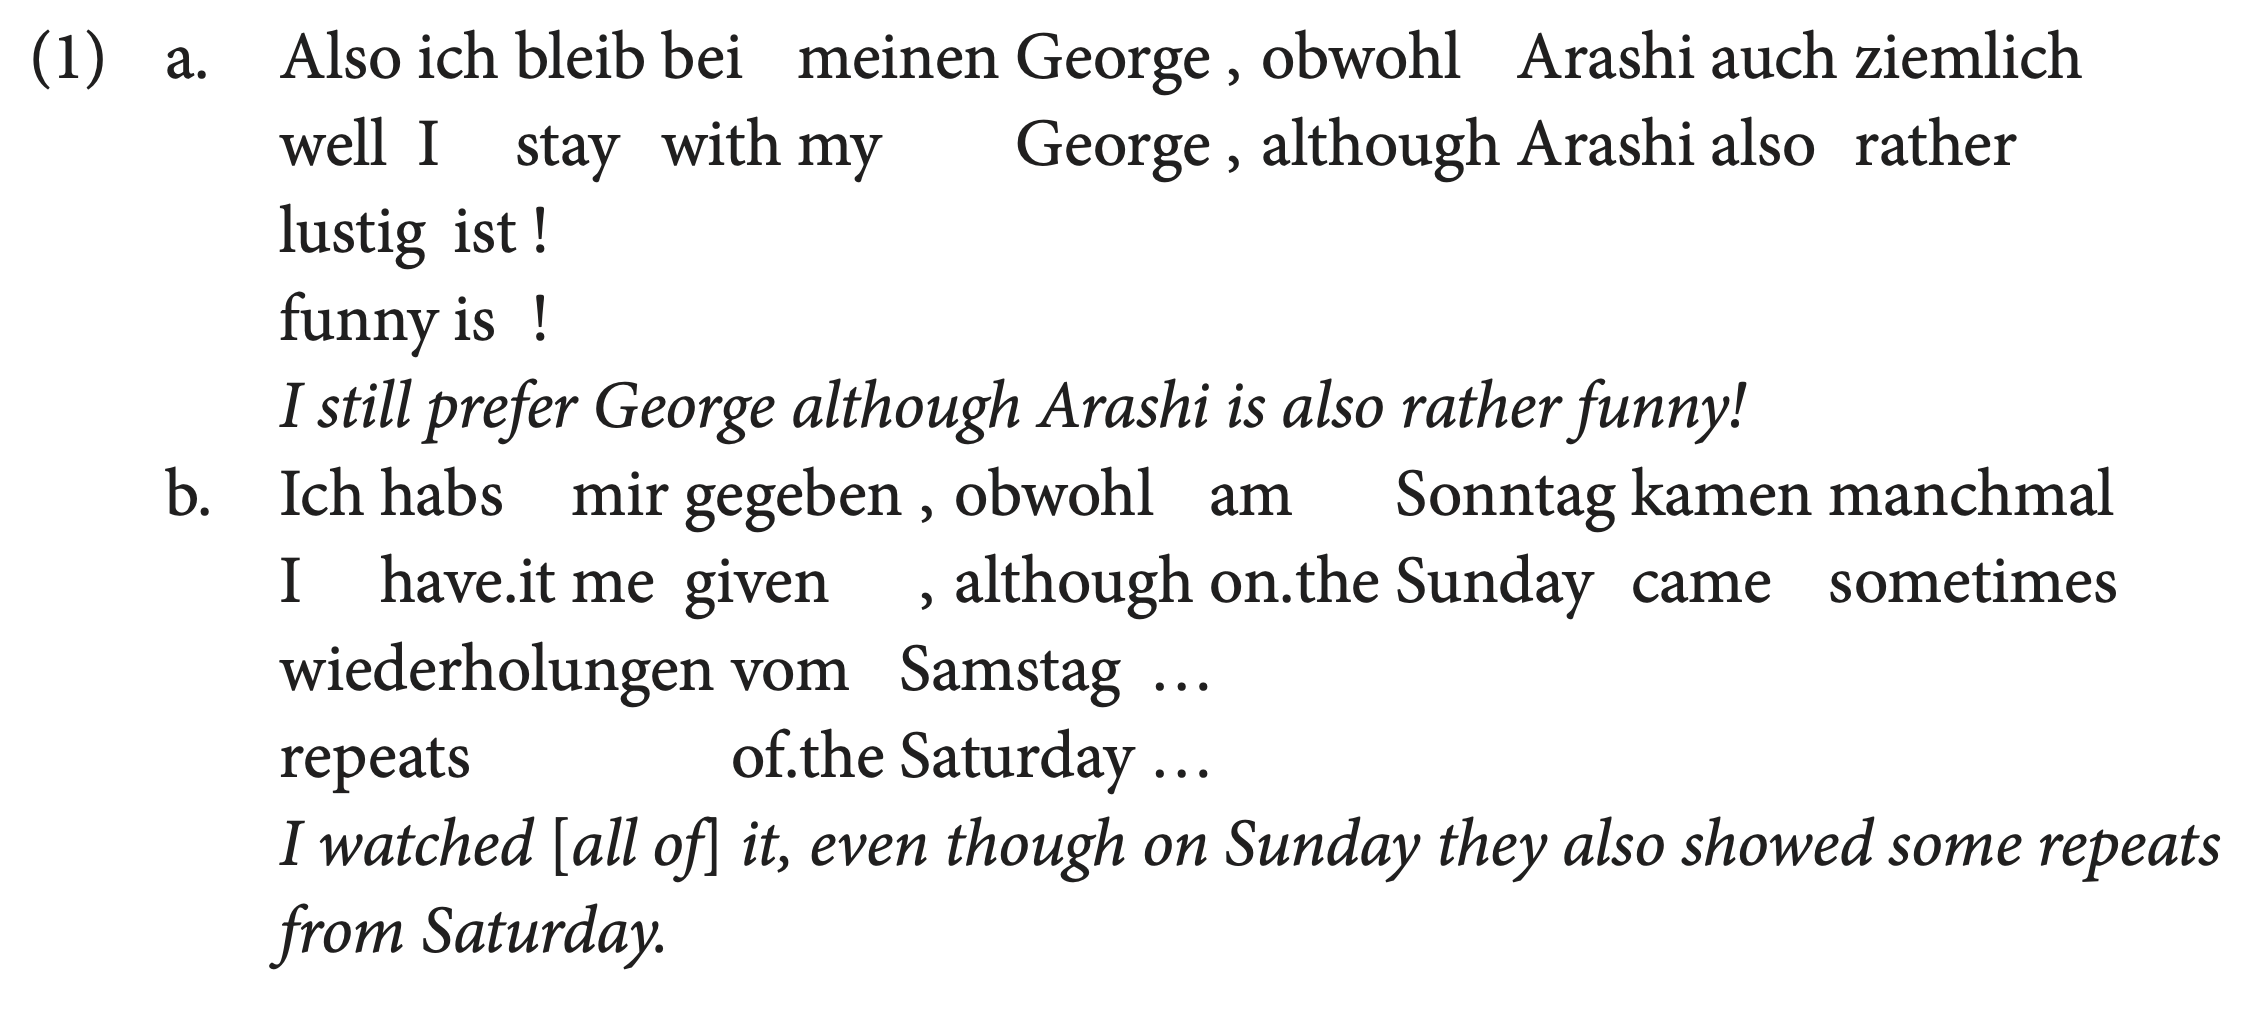
\includegraphics[width=0.7\textwidth]{\GRAPHPATH/obweil/01-obwohl}
\end{frame}

\begin{frame}
  {\textit{obwohl} und \textit{weil} mit V2}
  \centering 
  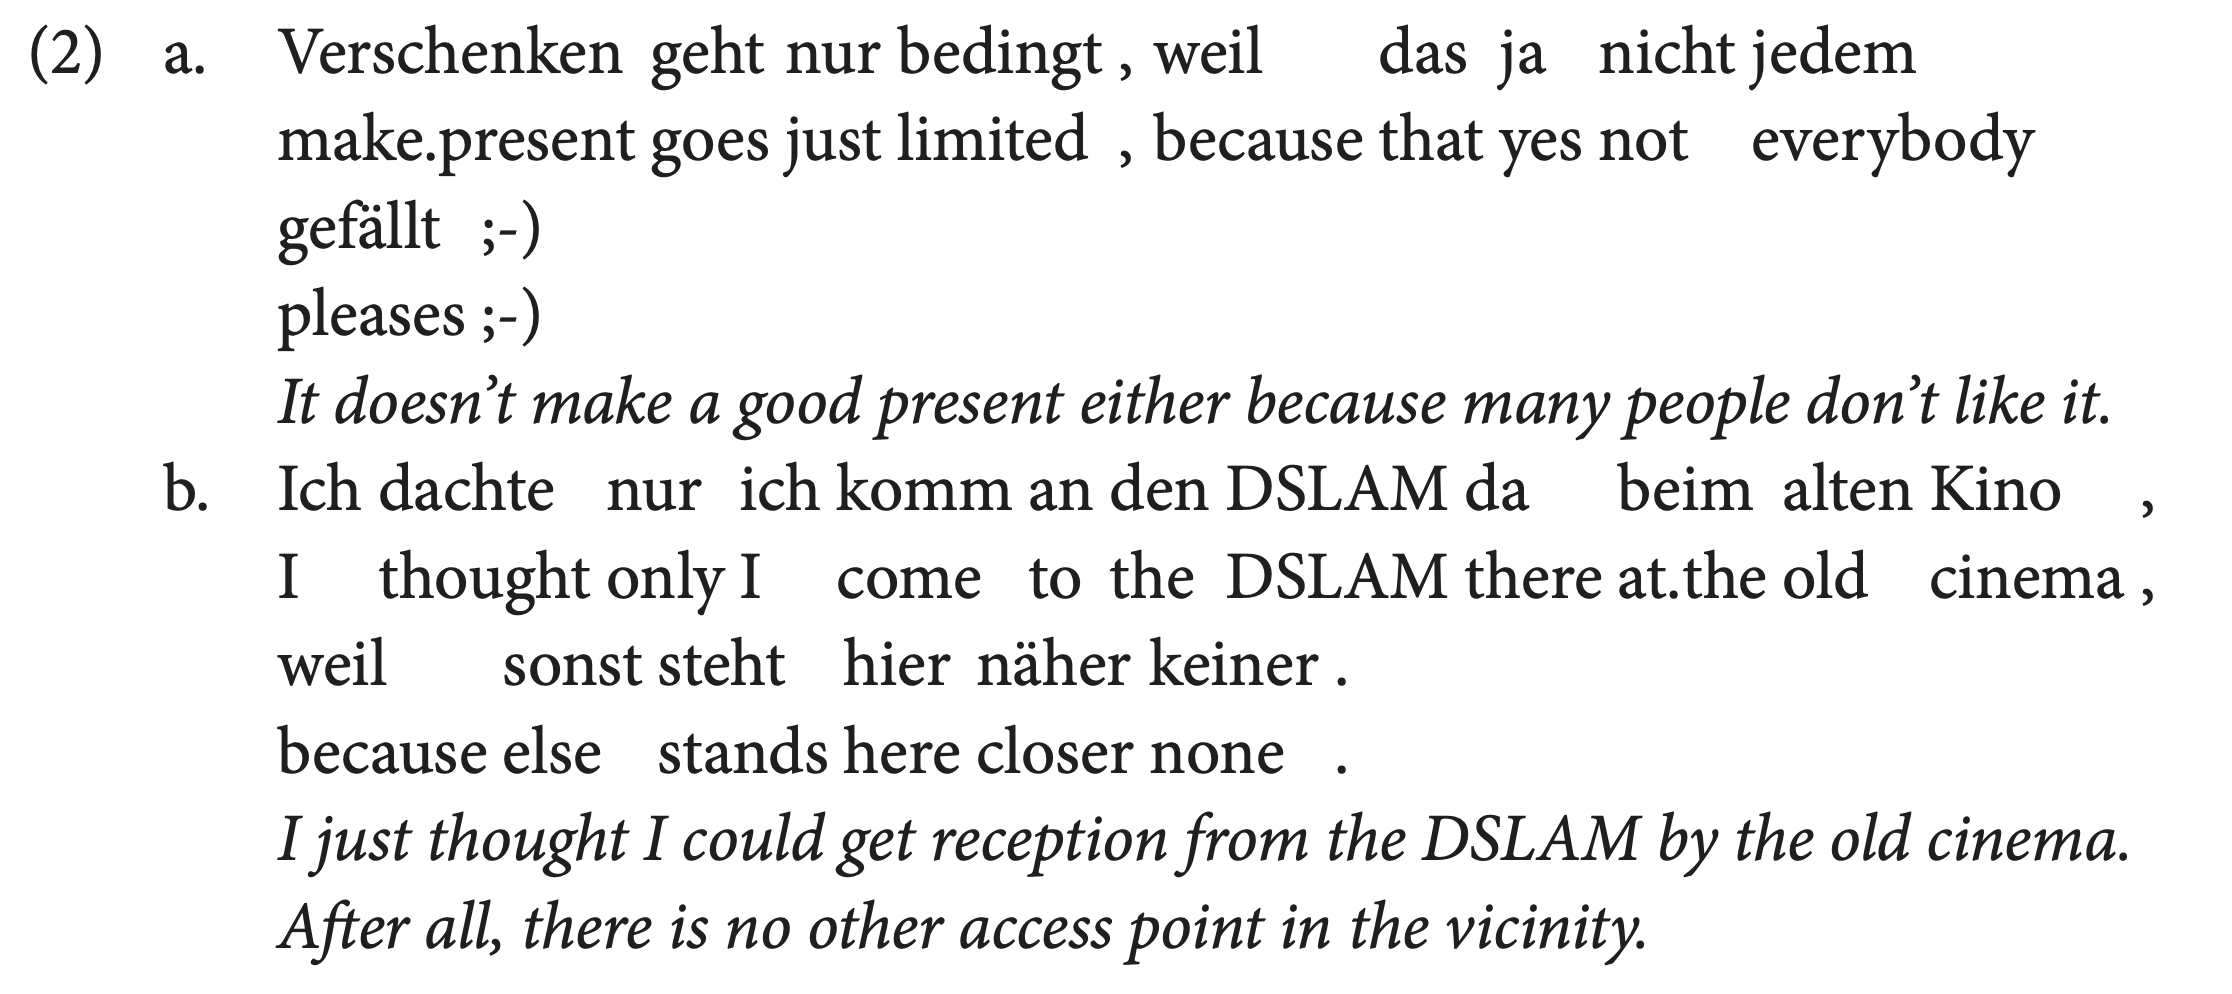
\includegraphics[width=0.7\textwidth]{\GRAPHPATH/obweil/01-weil}
\end{frame}

\begin{frame}
  {Variation der Interpunktion (Beispiele)}
  \centering 
  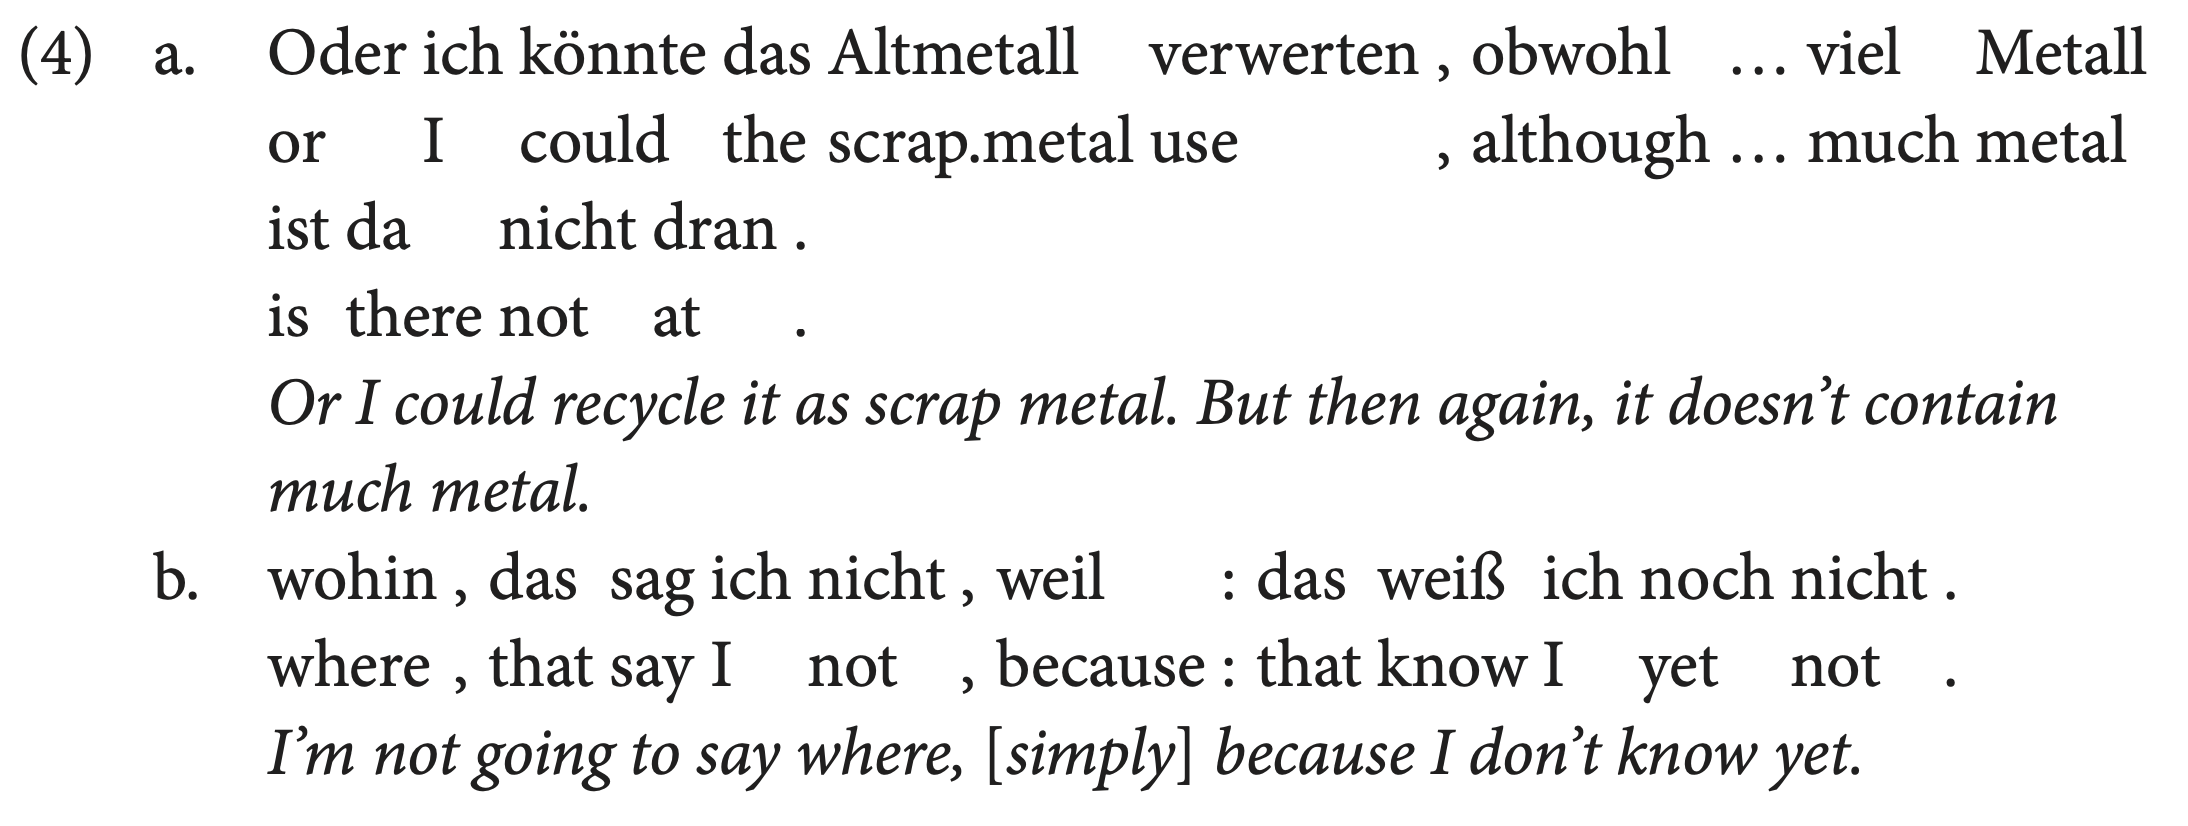
\includegraphics[width=0.7\textwidth]{\GRAPHPATH/obweil/02-interpunktion}
\end{frame}

\begin{frame}
  {Unabhängigkeit von Sätzen}
  \centering 
  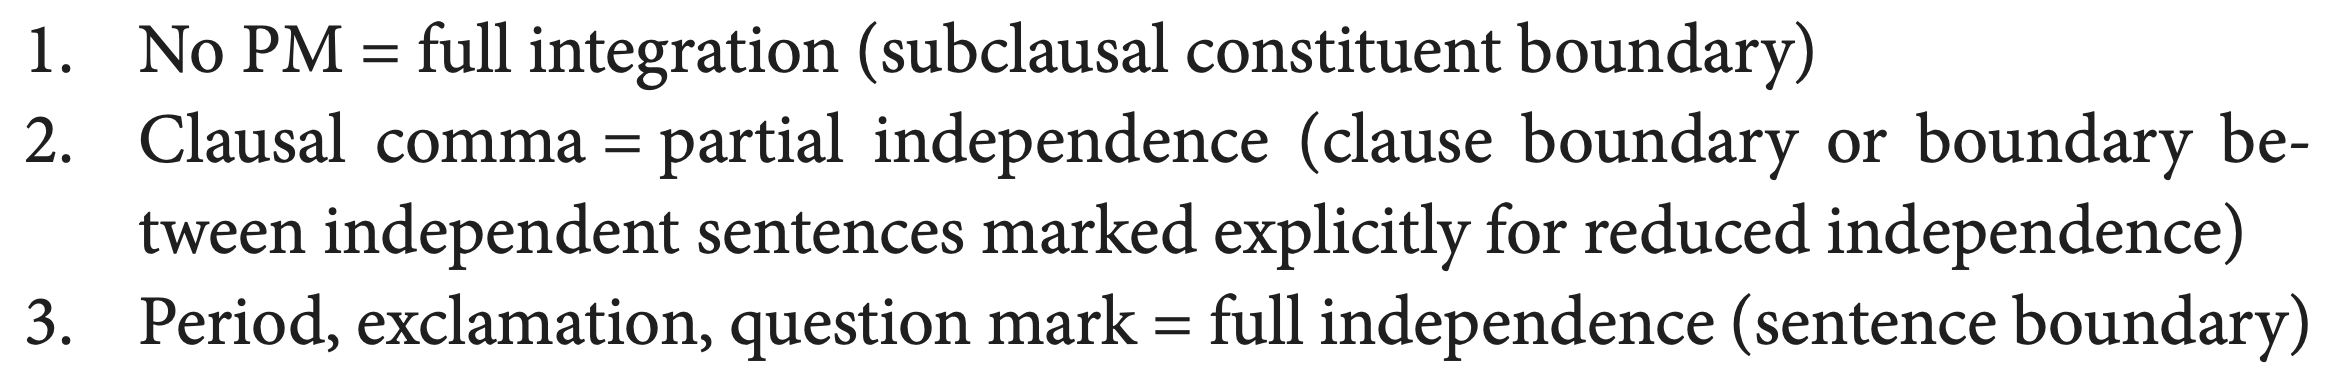
\includegraphics[width=0.7\textwidth]{\GRAPHPATH/obweil/03-independence} 
\end{frame}

\begin{frame}
  {Empirischer Befund I | Satzinitiale Partikeln}
  \centering 
  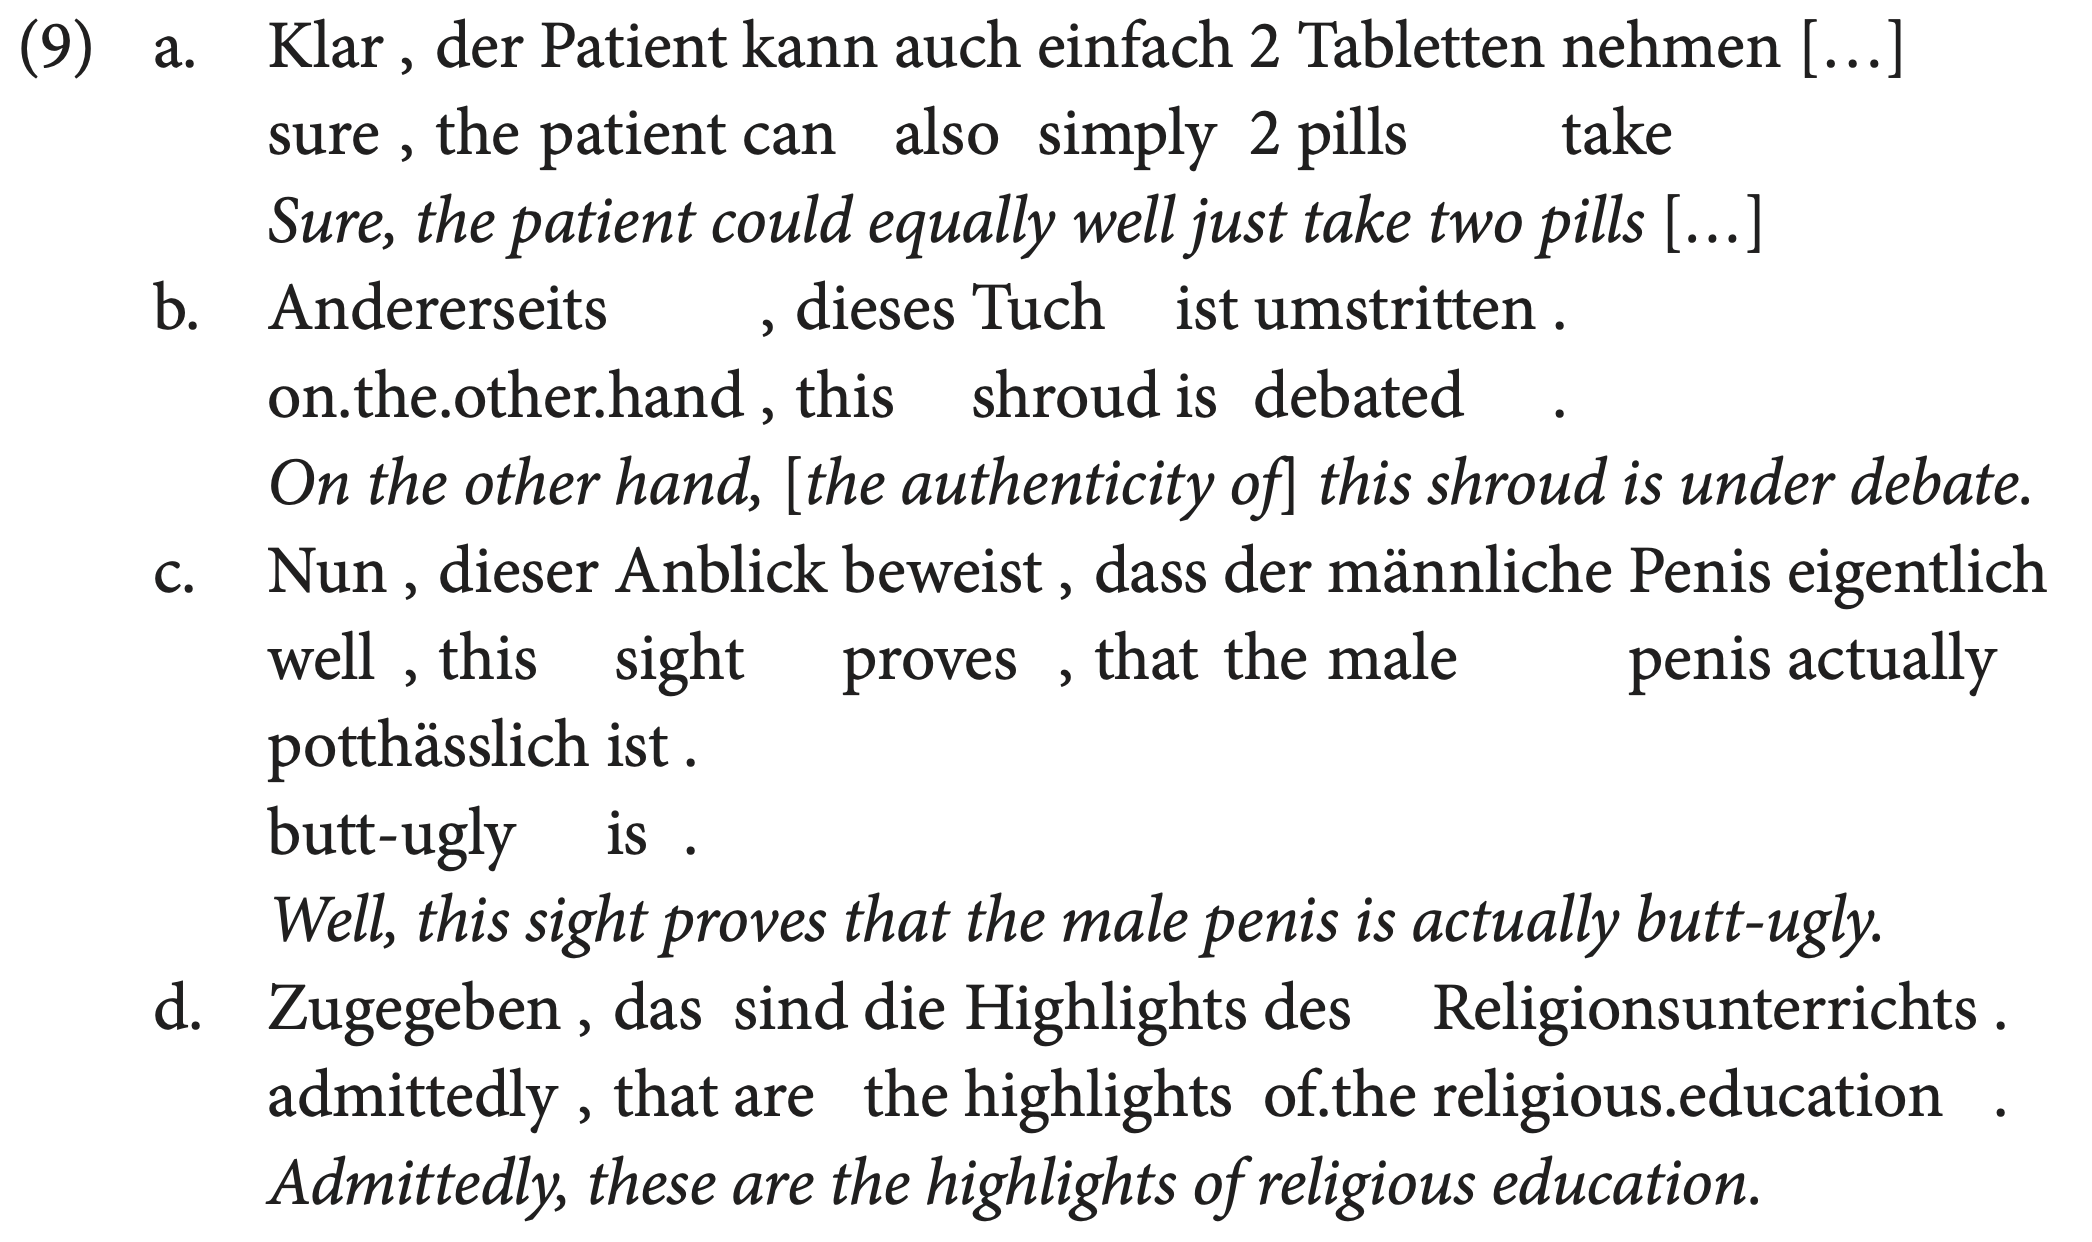
\includegraphics[width=0.7\textwidth]{\GRAPHPATH/obweil/04-satzinitial}
\end{frame}

\begin{frame}
  {Empirischer Befund II/1 | Wortverteilung bei Doppelpunkt}
  \centering 
  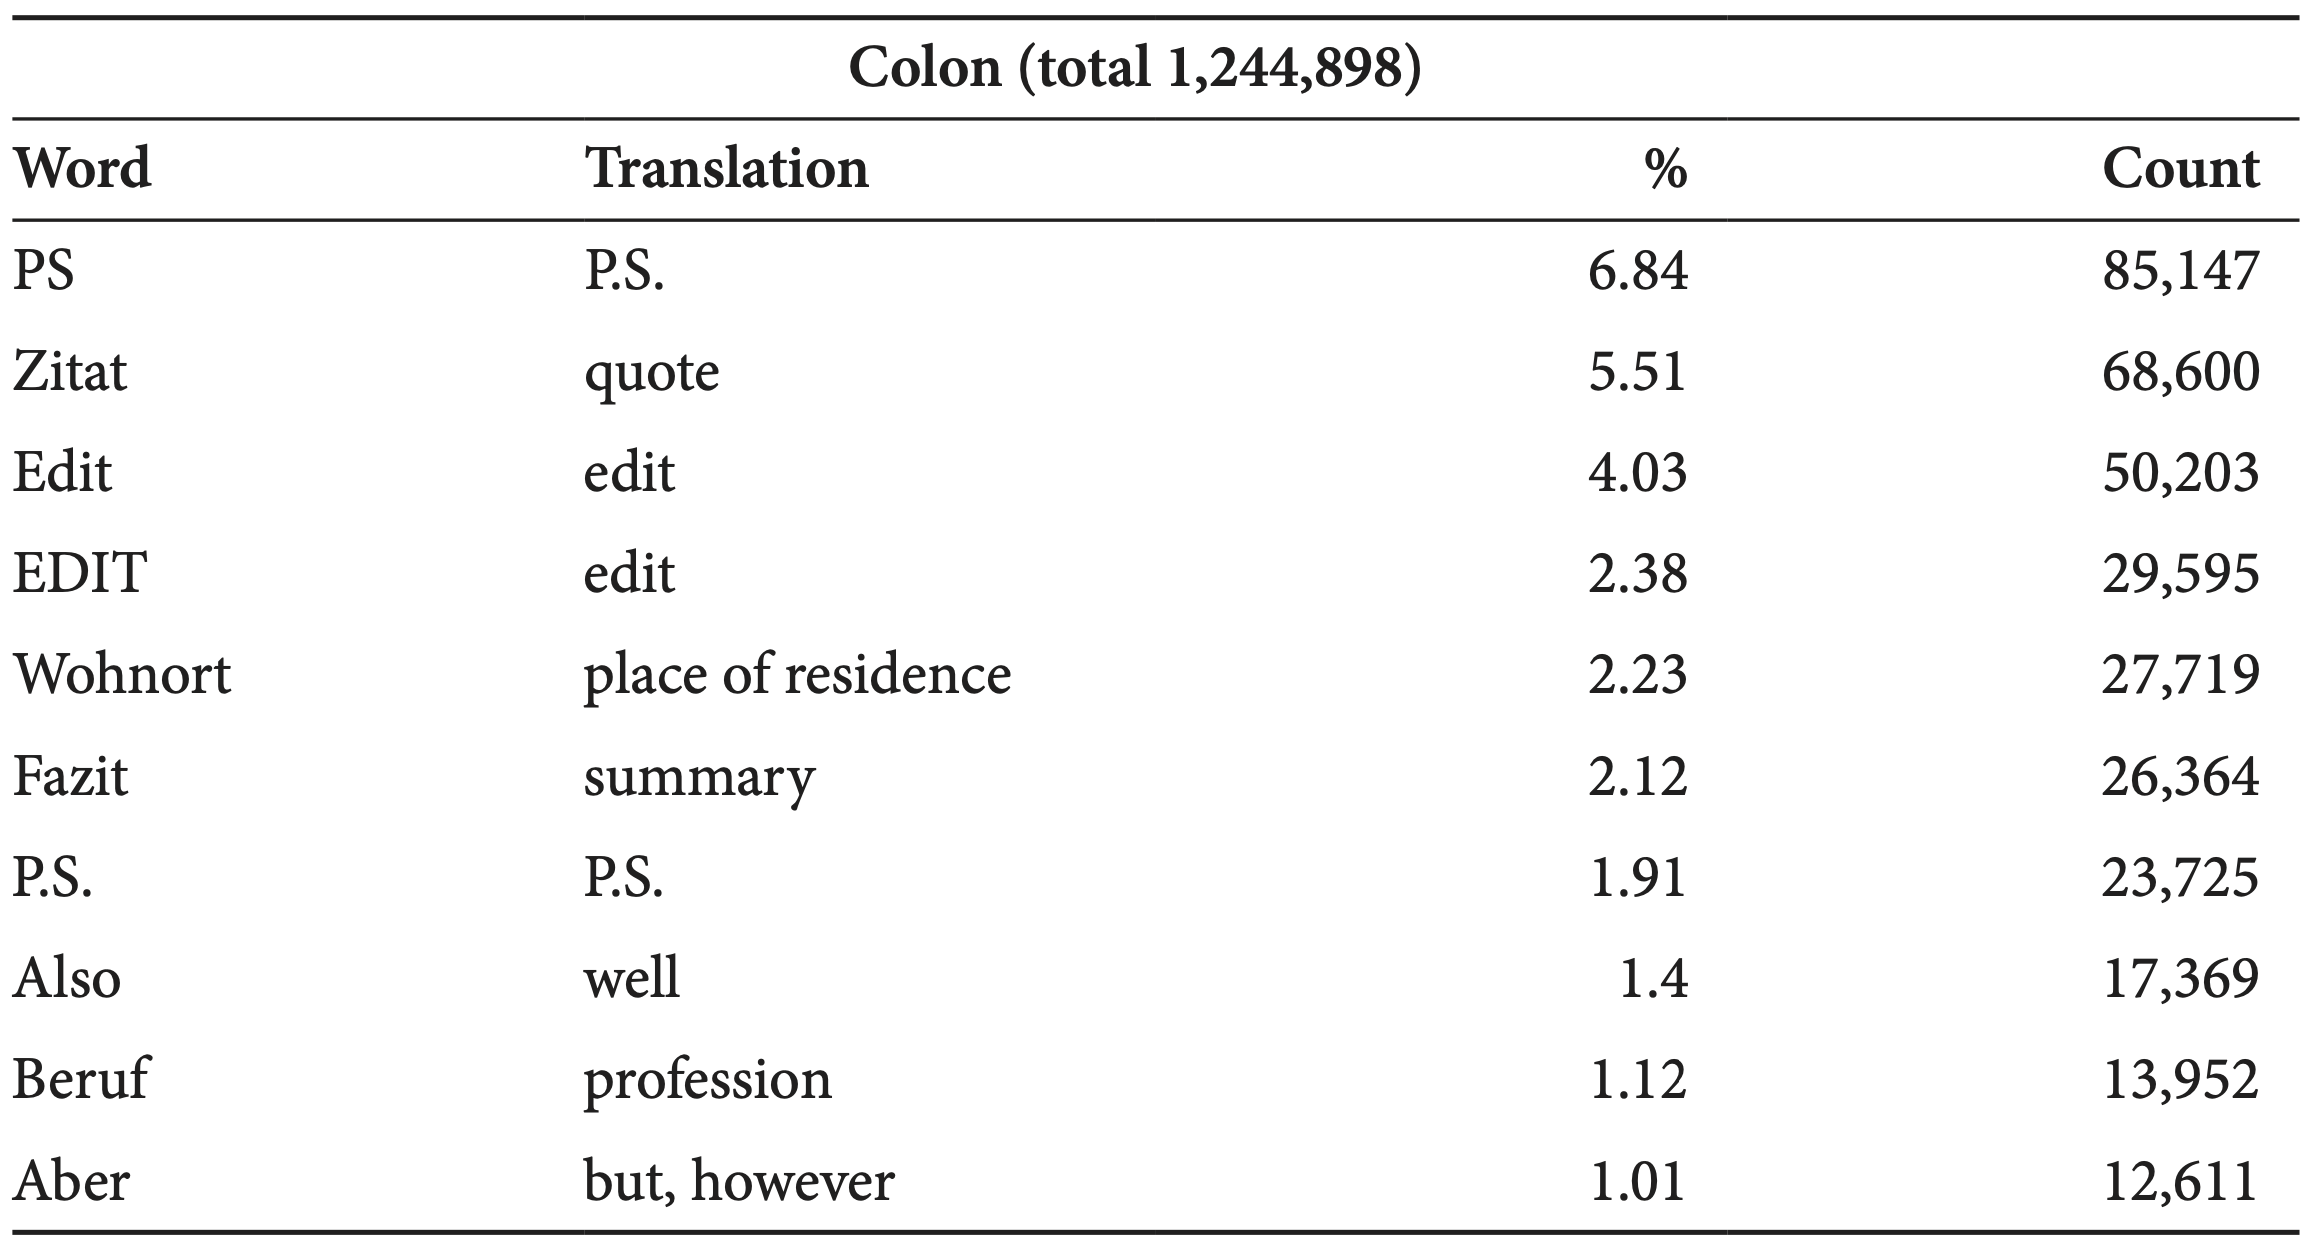
\includegraphics[width=0.7\textwidth]{\GRAPHPATH/obweil/05-colon}
\end{frame}

\begin{frame}
  {Empirischer Befund II/2 | Wortverteilung bei Komma}
  \centering 
  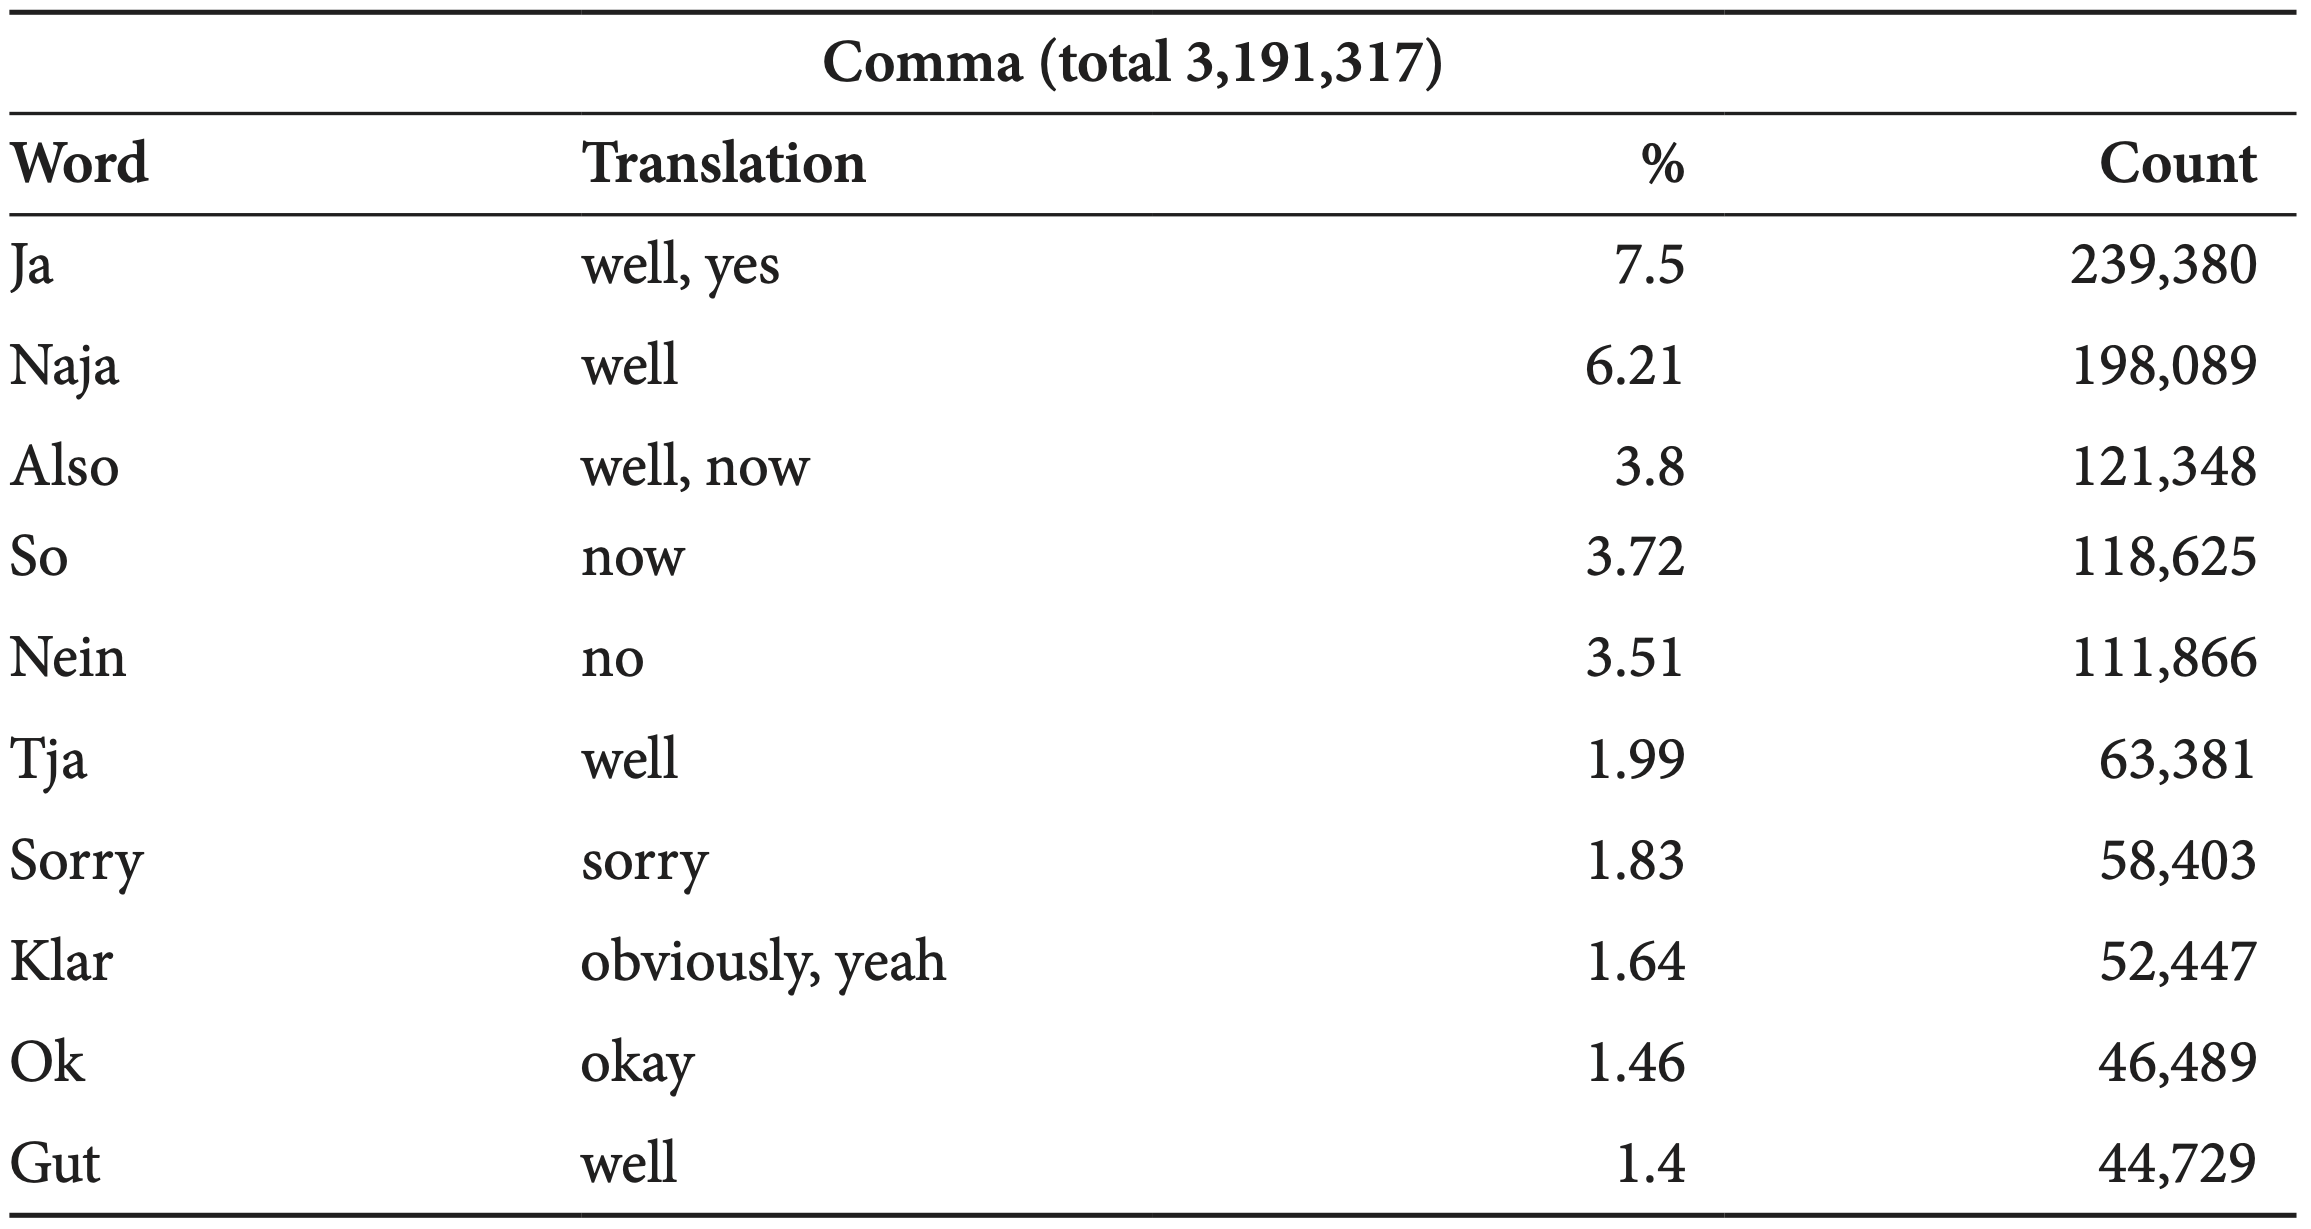
\includegraphics[width=0.7\textwidth]{\GRAPHPATH/obweil/05-comma}
\end{frame}

\begin{frame}
  {Empirischer Befund II/3 | Wortverteilung bei Bindestrich}
  \centering 
  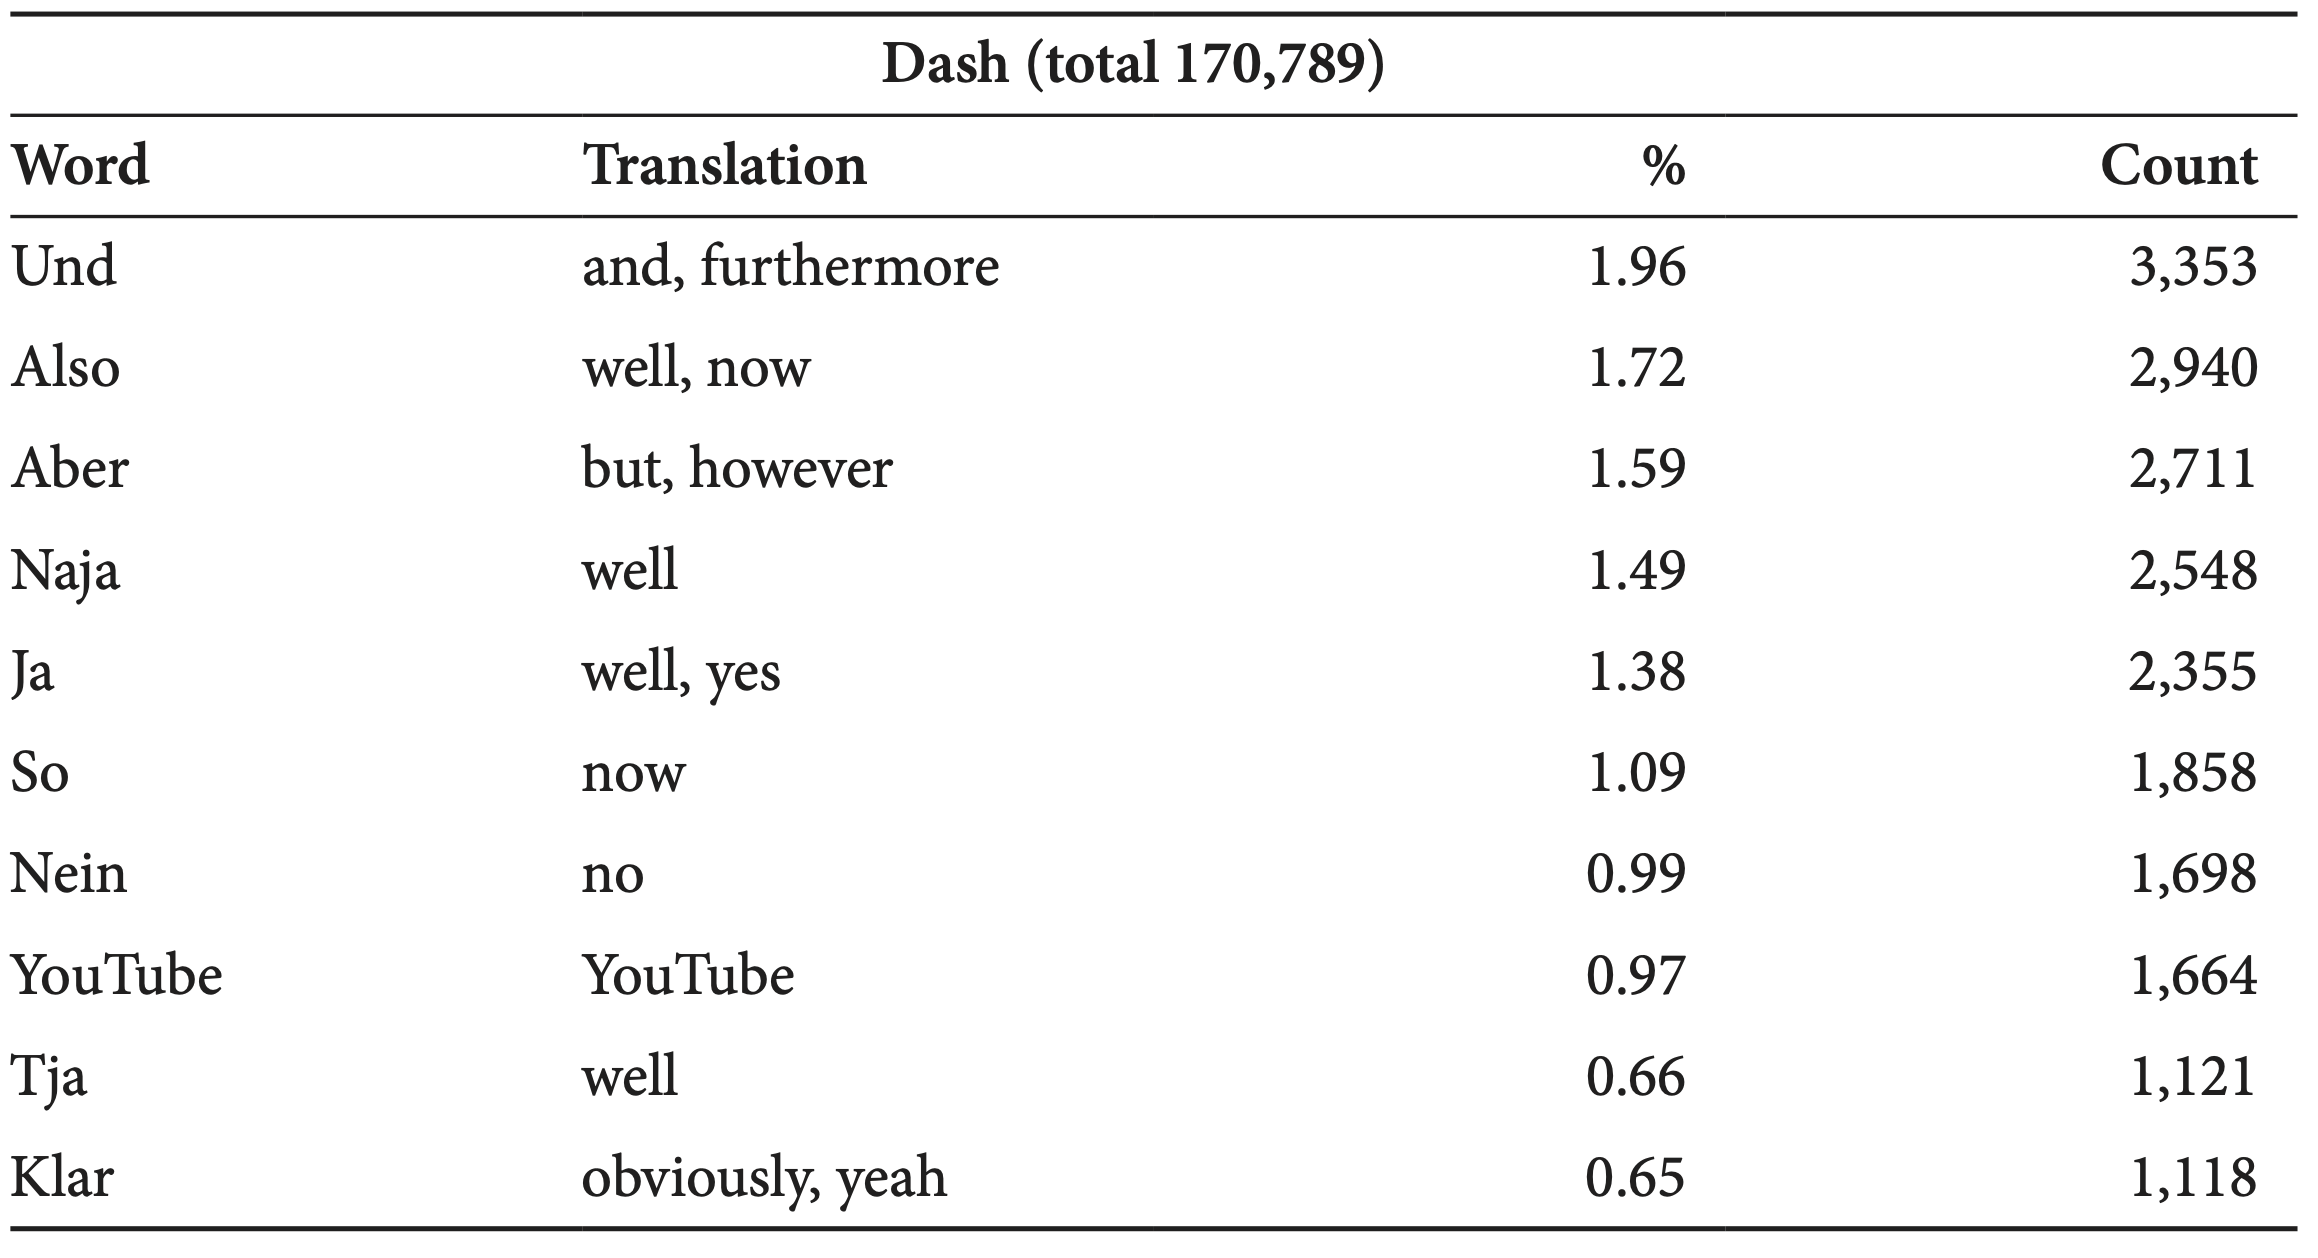
\includegraphics[width=0.7\textwidth]{\GRAPHPATH/obweil/05-dash}
\end{frame}

\begin{frame}
  {Empirischer Befund II/4 | Wortverteilung bei Dreipunkt}
  \centering 
  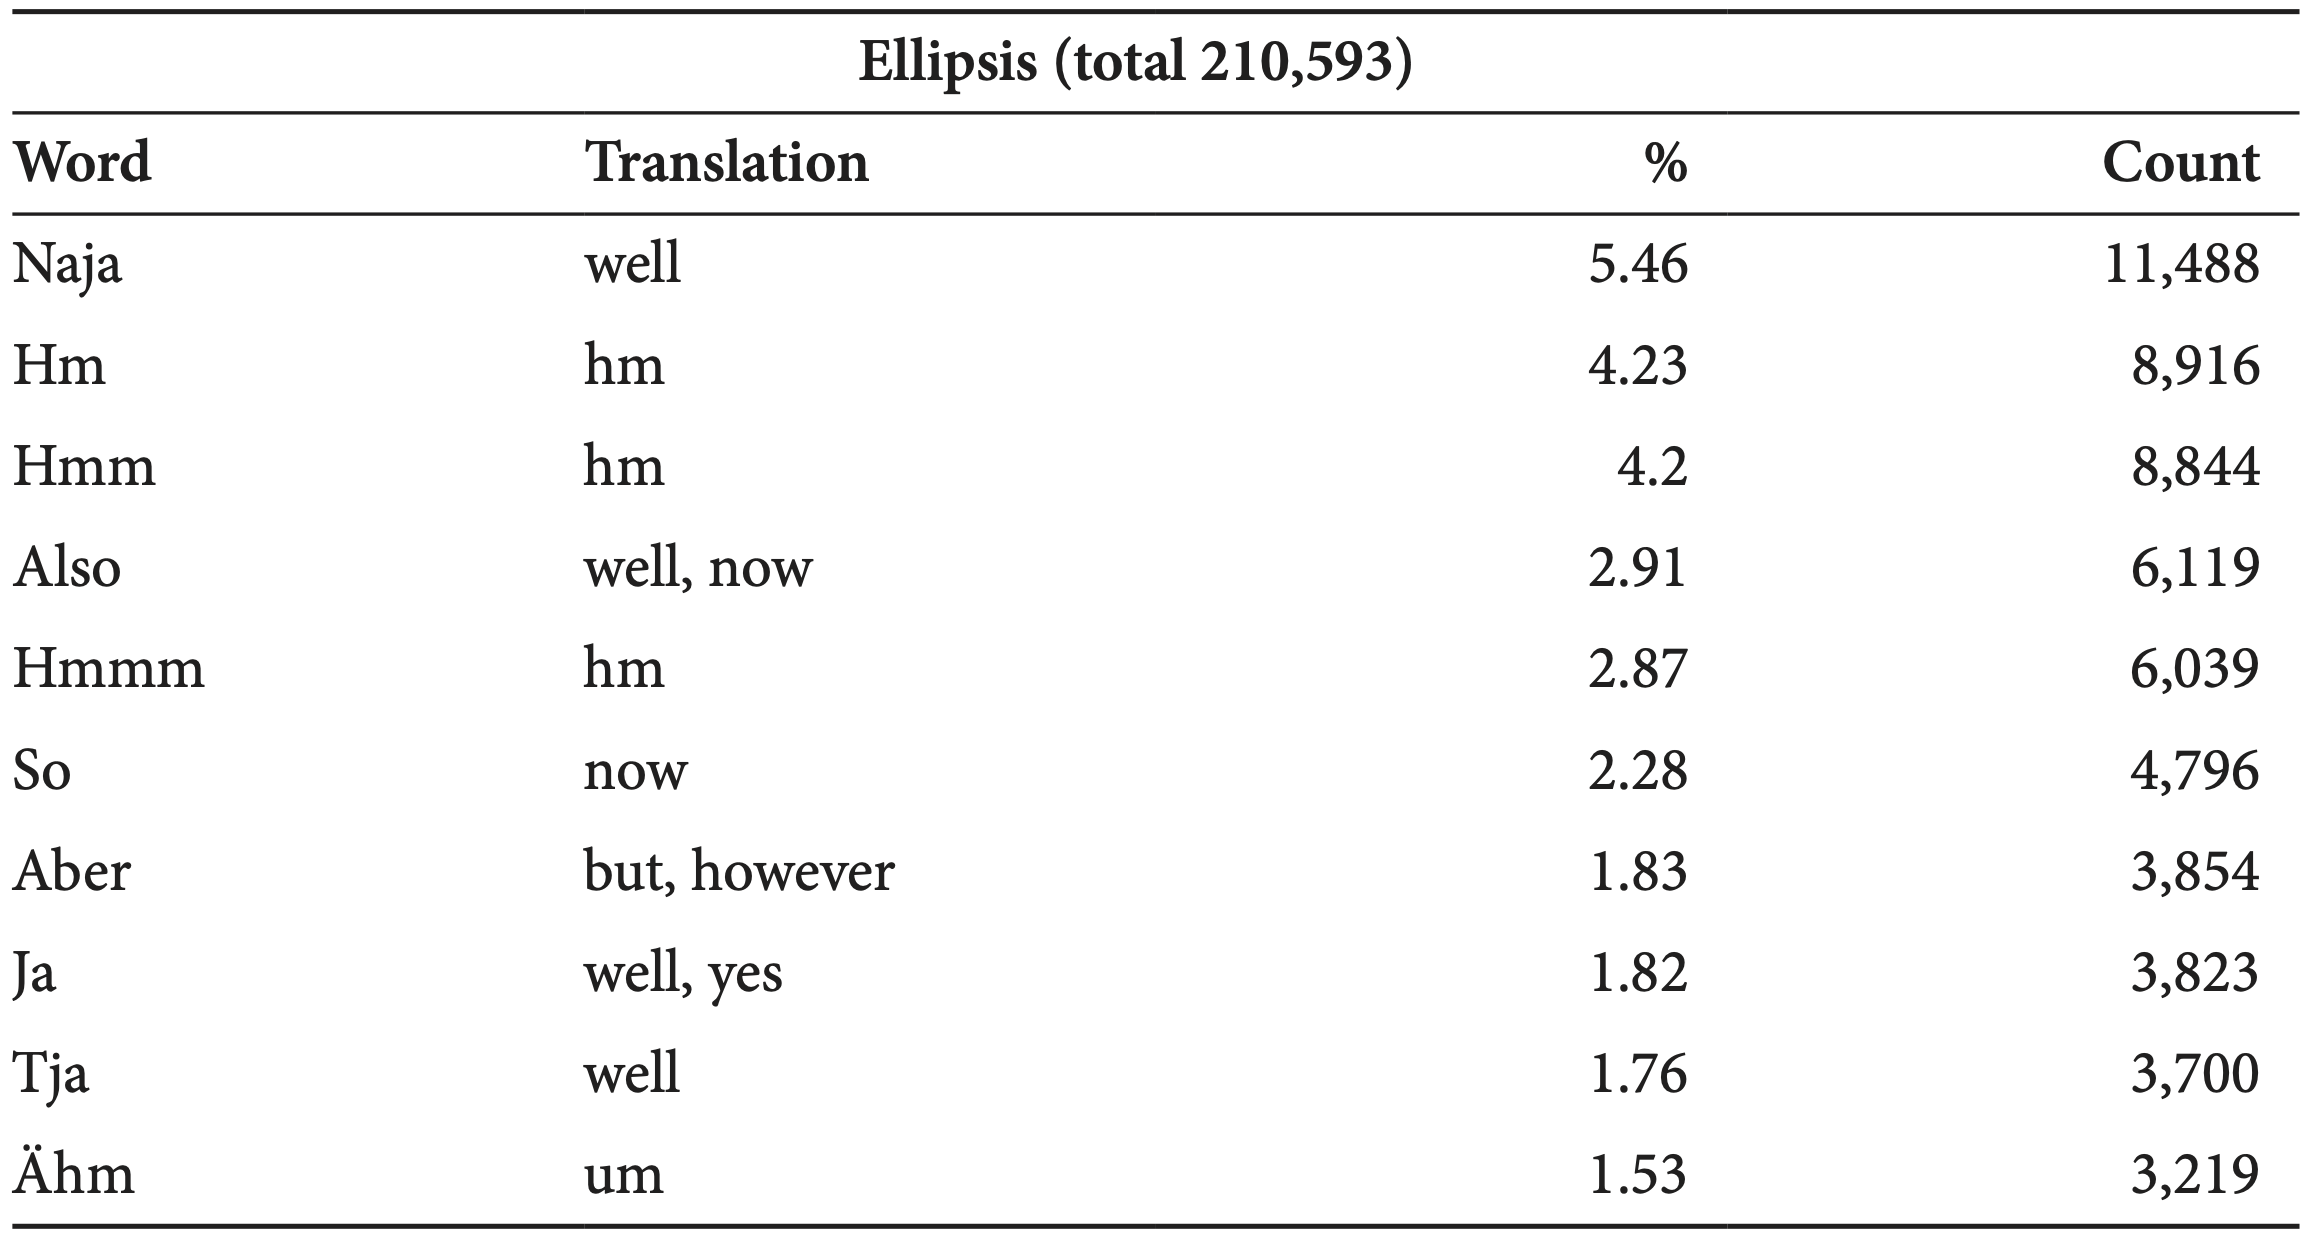
\includegraphics[width=0.7\textwidth]{\GRAPHPATH/obweil/05-ellipsis}
\end{frame}

\begin{frame}
  {Empirischer Befund III/1 | Links von \textit{obwohl}\slash \textit{weil}}
  \centering 
  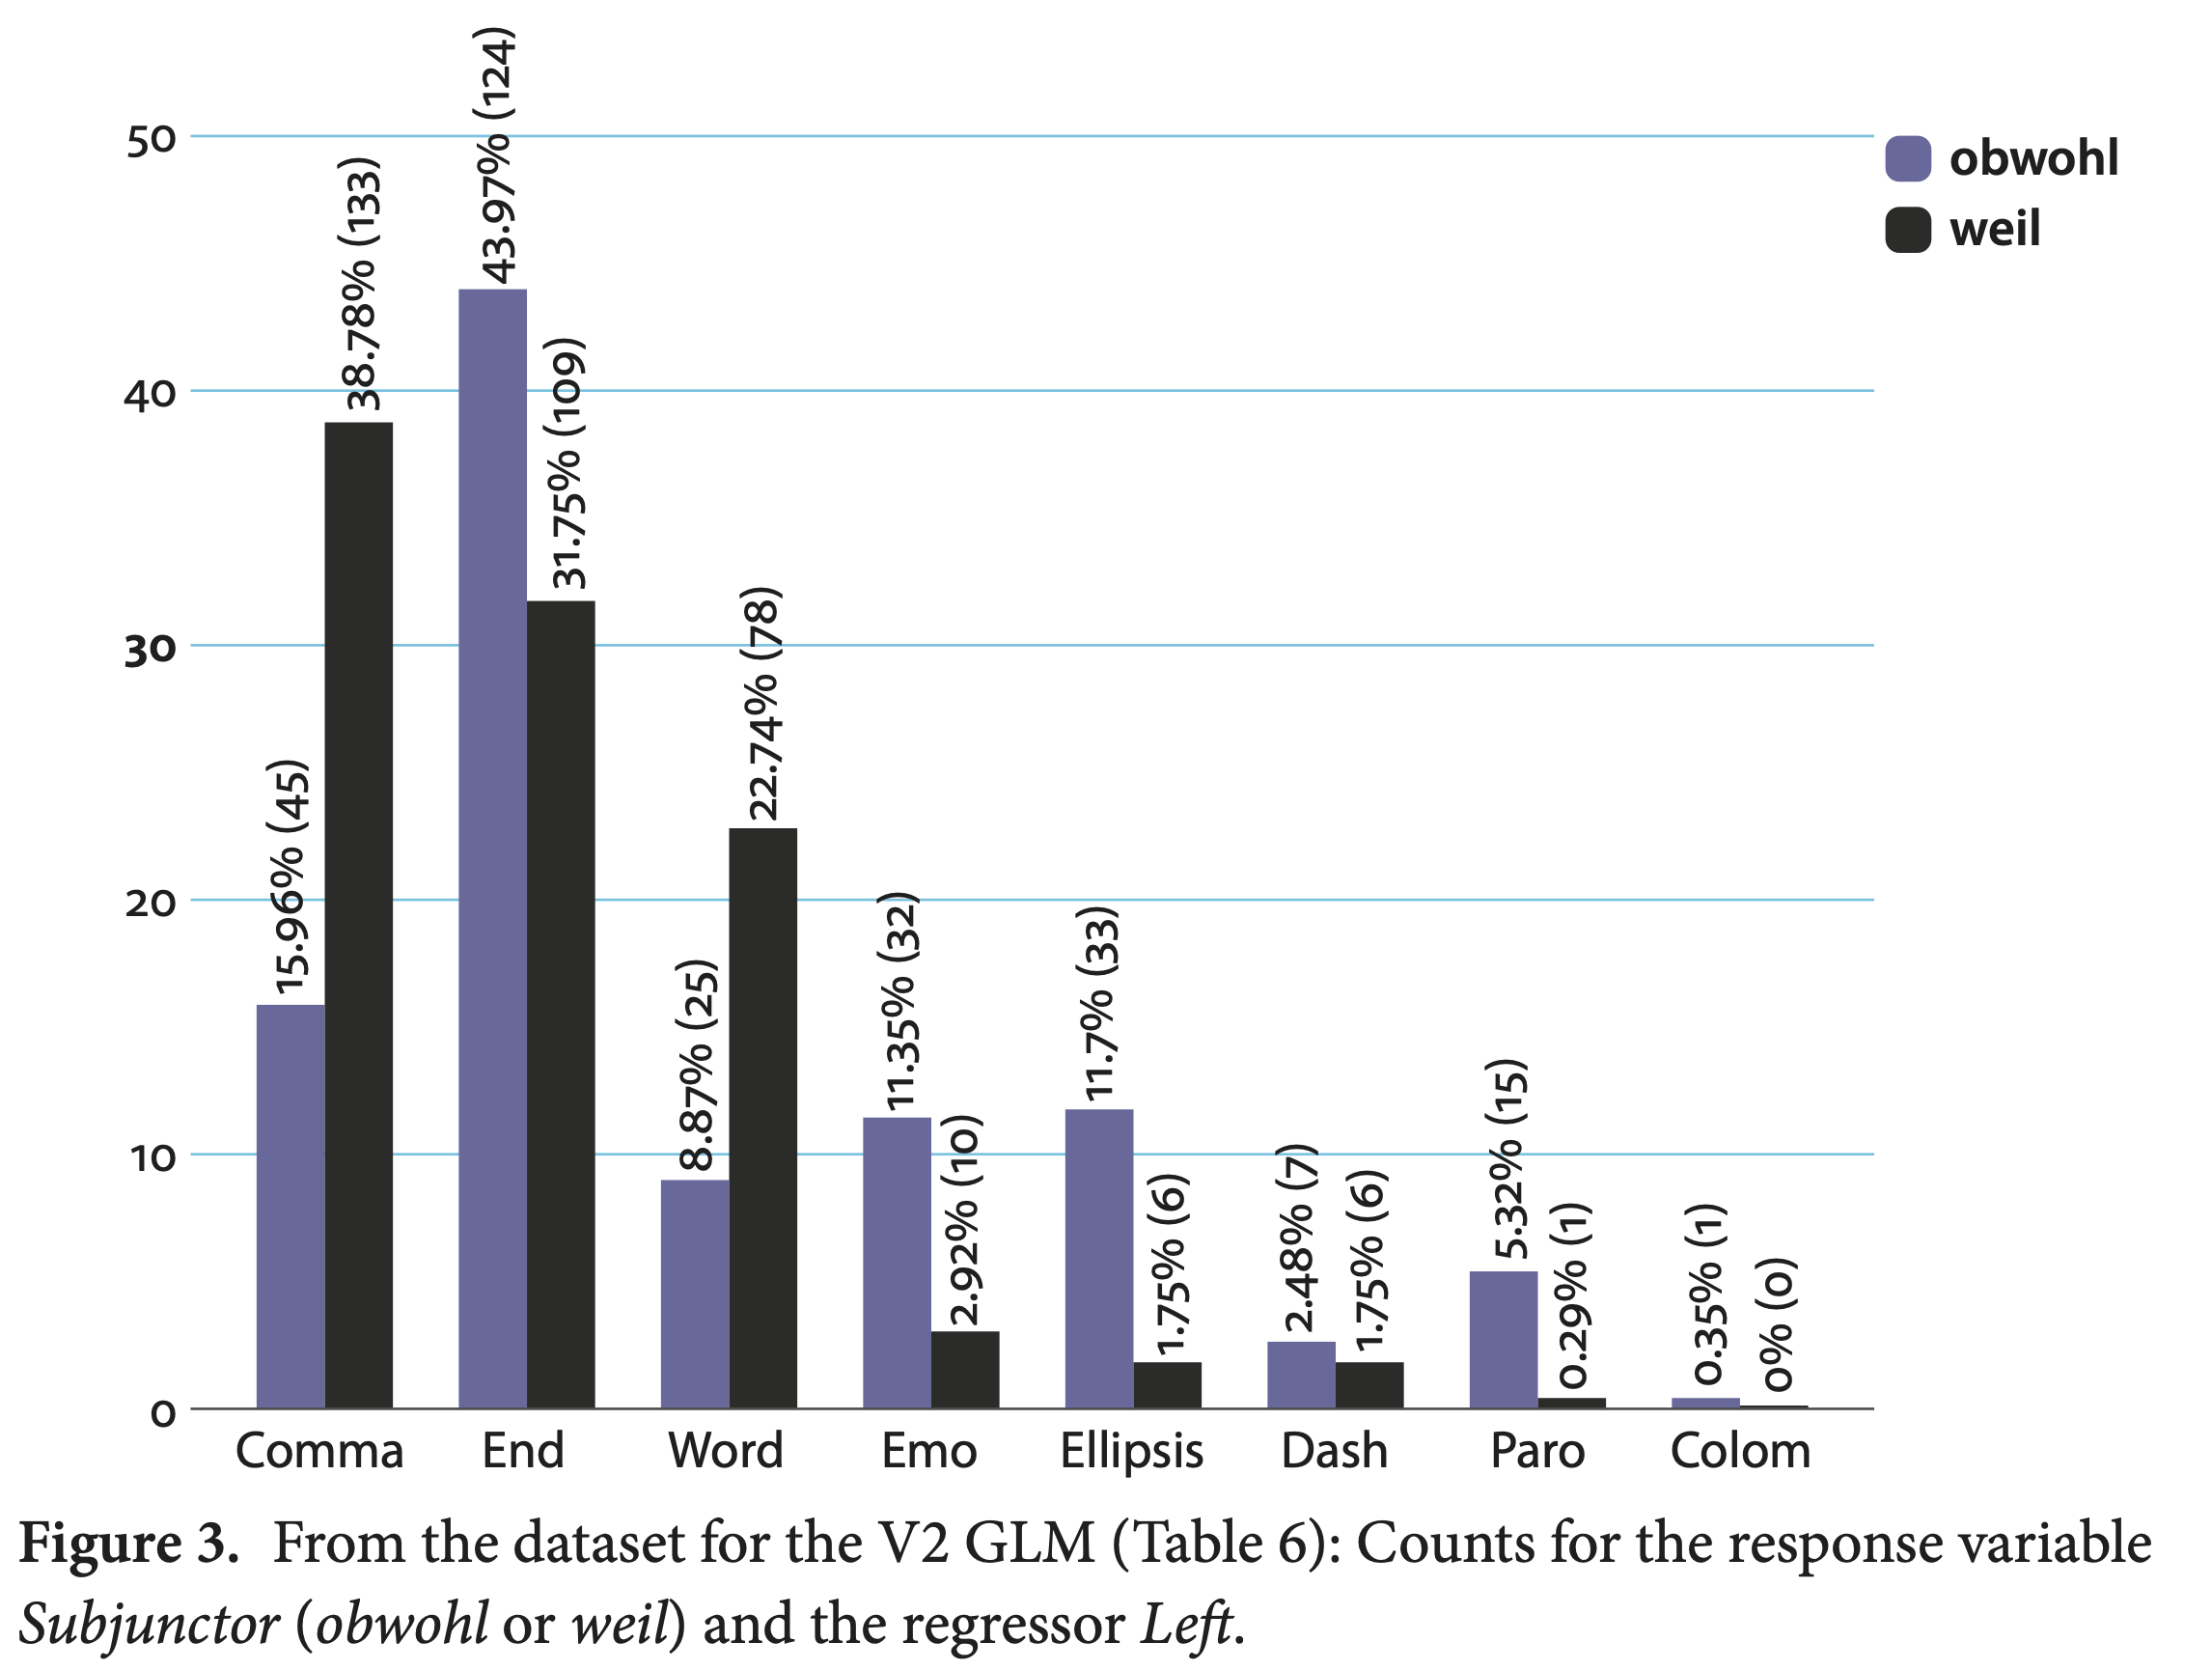
\includegraphics[width=0.7\textwidth]{\GRAPHPATH/obweil/06-left}
\end{frame}

\begin{frame}
  {Empirischer Befund III/2 | Rechts von \textit{obwohl}\slash \textit{weil}}
  \centering 
  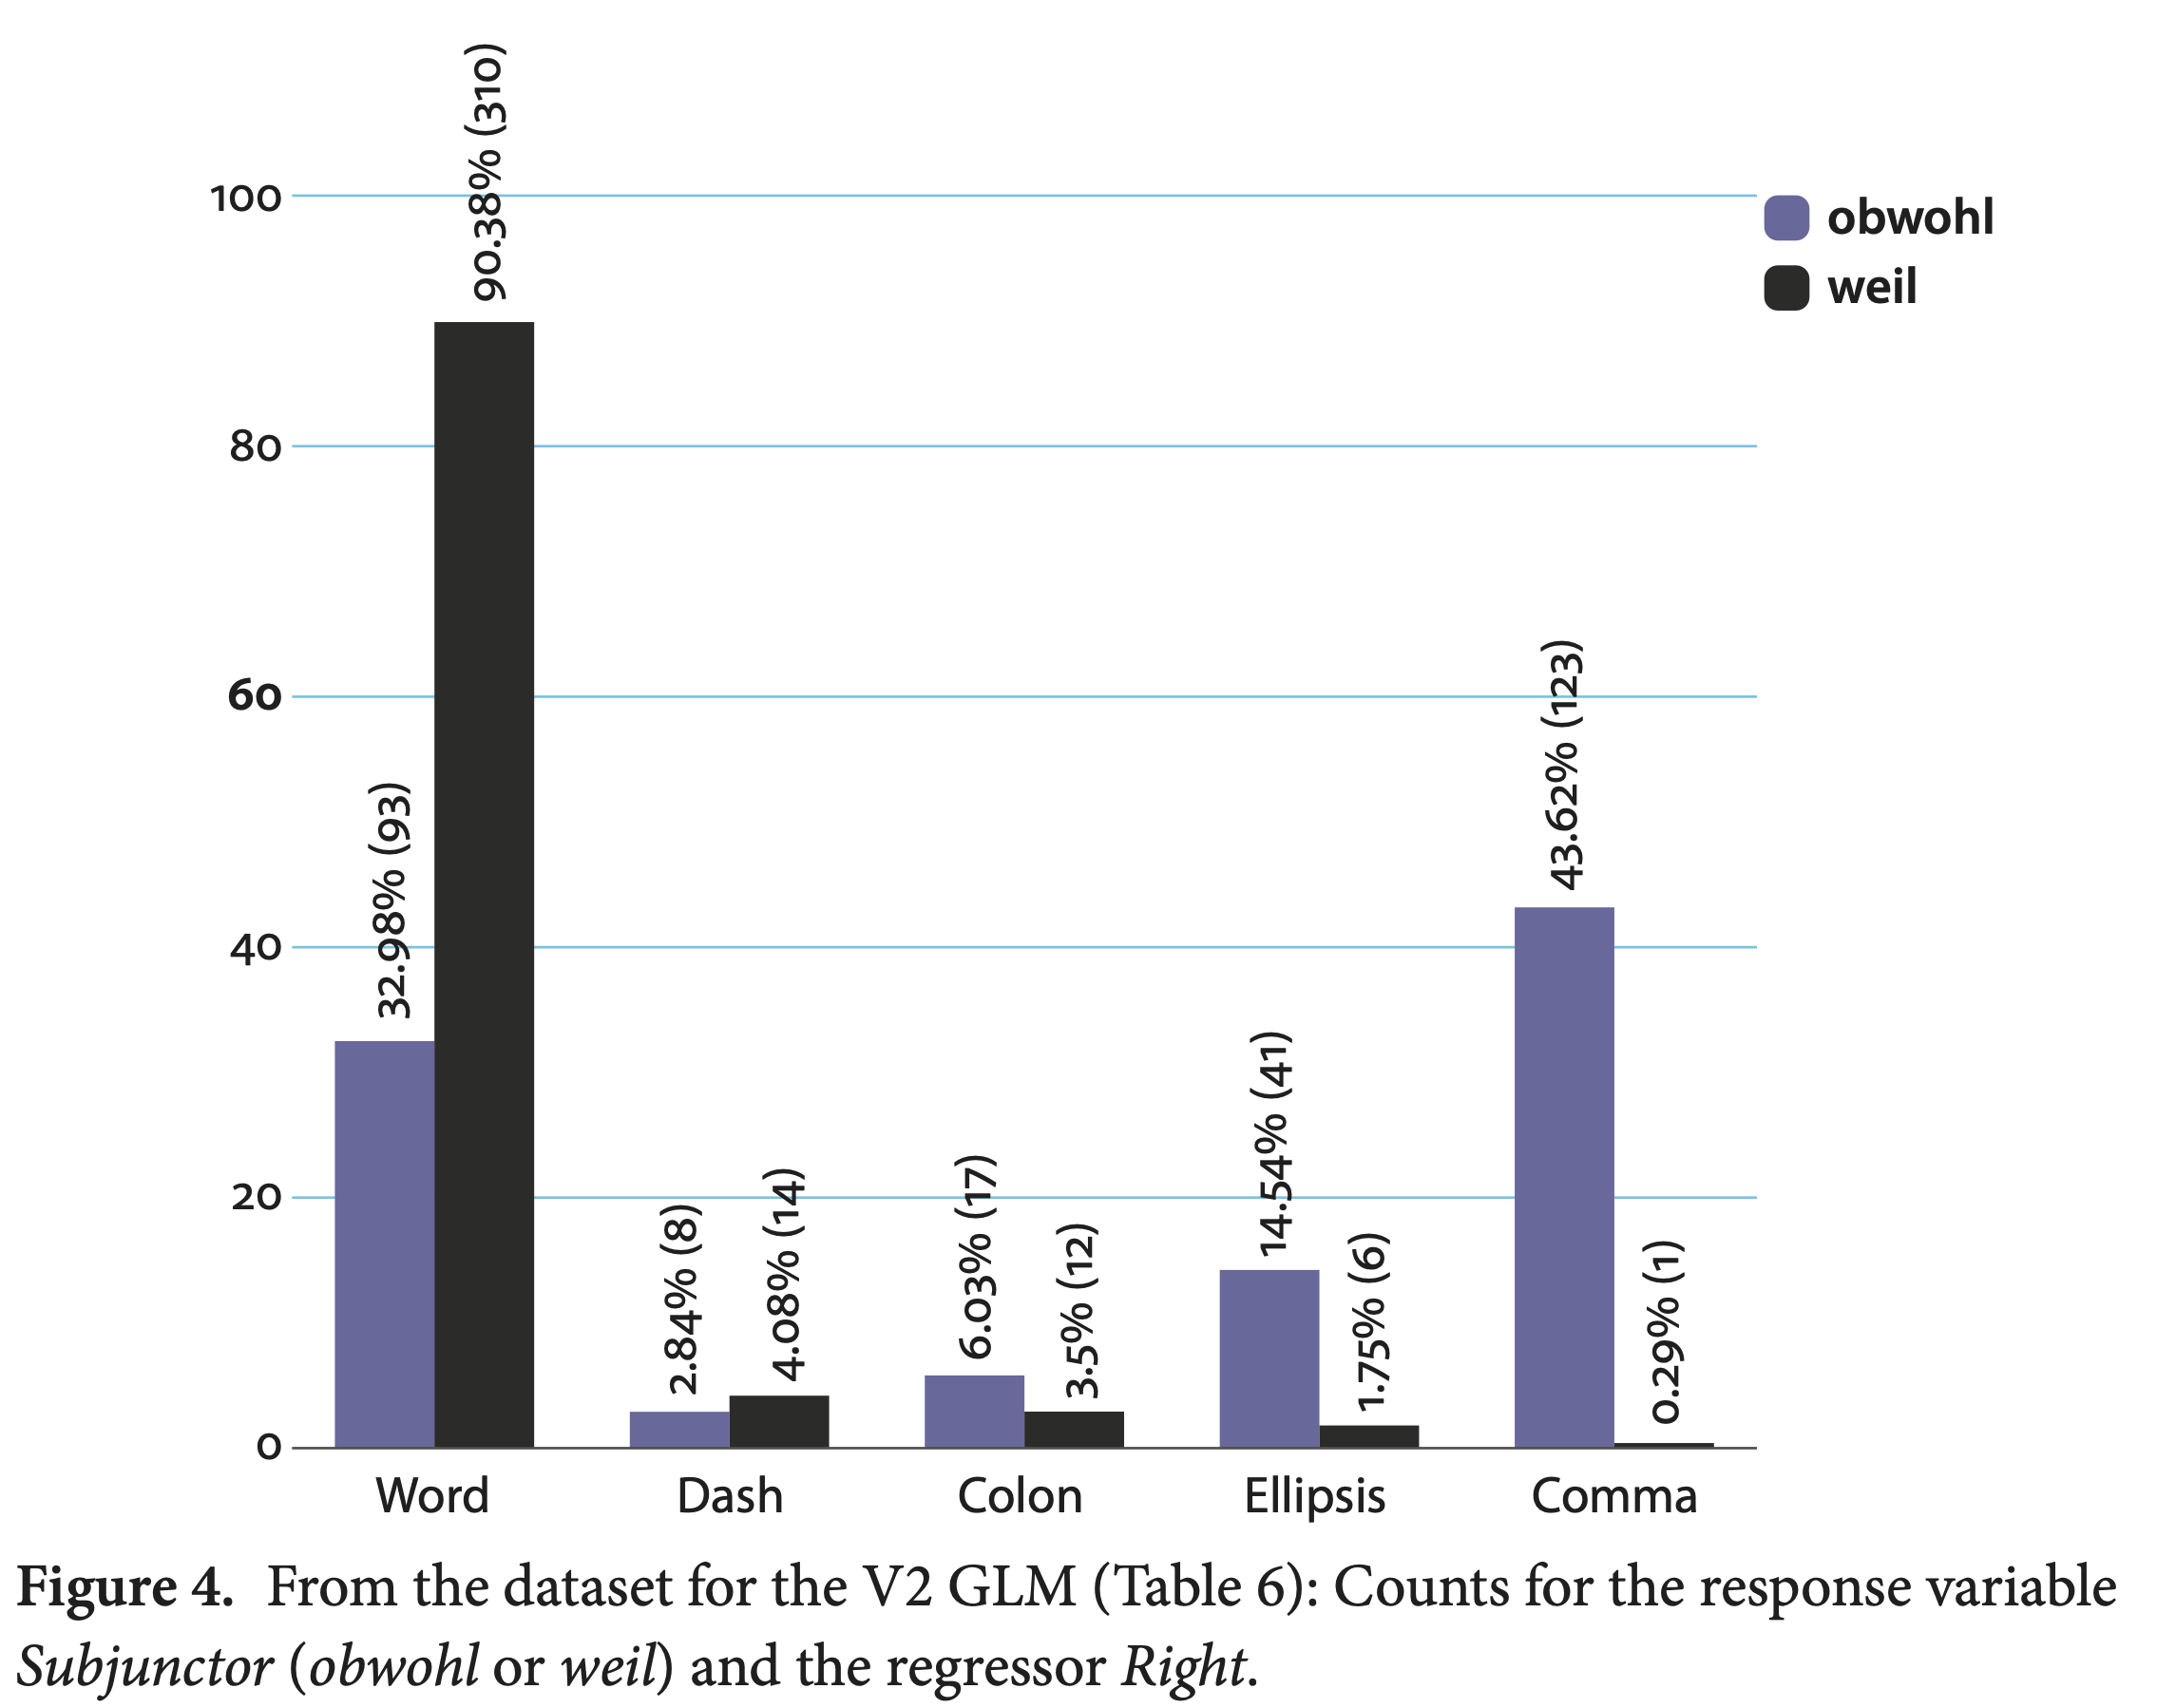
\includegraphics[width=0.7\textwidth]{\GRAPHPATH/obweil/06-right}
\end{frame}

\begin{frame}
  {Ergebnisse}
  \textit{obwohl} und \textit{weil} mit V2-Satzstellung\\
  \Zeile
  \begin{itemize}[<+->]
    \item \textit{obwohl}
      \begin{itemize}[<+->]
        \item leitet mehr unabhängige Sätze ein
        \item wird öfter vom Komma gefolgt
        \item Status | \alert{eher Diskurspartikel außerhalb des Satzes}
        \item ähnlich \textit{ja}, \textit{naja}, \textit{also}, \textit{klar}
      \end{itemize}
      \Zeile
    \item \textit{weil}
      \begin{itemize}[<+->]
        \item folgt auch bei V2 eher einem Komma
        \item oder ganz ohne Interpunktion links
        \item Komma folgt seltener
        \item Status | \alert{eher Konnektor im Konnektorfeld}
        \item ähnlich \textit{denn}
      \end{itemize}
  \end{itemize}
\end{frame}



\ifdefined\TITLE
  \section{Nächste Woche | Überblick}

  \begin{frame}
    {Der ungefähre Semesterplan}
    \begin{enumerate}[<+->]
      \item Graphematik und Schreibprinzipien
      \item Wiederholung -- Phonetik
      \item Wiederholung -- Phonologie
      \item Phonographisches Schreibprinzip -- Konsonanten
      \item Phonographisches Schreibprinzip -- Vokale
      \item Silben und Dehnungsschreibungen
      \item Eszett, Dehnung und Konstanz
      \item Spatien und Majuskeln
      \item Komma
      \item \alert{Punkt und sonstige Interpunktion}
    \end{enumerate}
  \end{frame}
\fi

  \let\subsection\section\let\section\woopsi
  
  \section{10. Punkt und sonstige Interpunktion}
  \let\woopsi\section\let\section\subsection\let\subsection\subsubsection
  \section{Übersicht}

\begin{frame}
  {Übersicht}
  \onslide<+->
  \begin{itemize}[<+->]
    \item \citet{Schaefer2018b}
  \end{itemize}
\end{frame}

\section[Wortzeichen]{Vergessen: Wortzeichen}

\begin{frame}
  {--}
  \onslide<+->
  \onslide<+->
  \begin{exe}
    \ex
    \begin{xlist}
      \ex[ ]{Wohnungstür}
      \ex[*]{Wohnung\orongsch{s}-Tür}
    \end{xlist}
    \ex
    \begin{xlist}
      \ex[ ]{Ofenkammer}
      \ex[?]{Ofen-Kammer}
    \end{xlist}
    \ex
    \begin{xlist}
      \ex[?]{Hornerschema}
      \ex[ ]{Horner-Schema}
    \end{xlist}
    \ex
    \begin{xlist}
      \ex[?]{Xylitsüßmittel}
      \ex[ ]{Xylit-Süßmittel}
    \end{xlist}
    \ex
    \begin{xlist}
      \ex[*]{Mallocexception}
      \ex[ ]{Malloc-Exception}
    \end{xlist}
  \end{exe}
\end{frame}

\begin{frame}
  {Der Bindestrich}
  \onslide<+->
  \begin{itemize}[<+->]
    \item Kompositum = \alert{ein} syntaktisches\slash prosodisches Wort,\\
      \onslide<+->
      \alert{zwei} phonologische\slash morphologische Wörter
      \Halbzeile
    \item Spatium | Trennung syntaktischer Wörter
      \Zeile
    \item Bindestrich | optionaler morpholgischer Trenner im Kompositum
      \begin{itemize}[<+->]
        \item weitgehend \rot{blockiert bei Fugenelemnt}
        \item prototypisch bei \alert{Eigennamenbeteiligung}
        \item prototypisch bei \alert{Lehnwortbeteiligung}
        \item präferierter bei stark \tuerkis{produktiver Bildung}
        \item präferierter bei \tuerkis{weniger integrierten Gliedern}
      \end{itemize}
  \end{itemize}
\end{frame}

\begin{frame}
  {`}
  \onslide<+->
  \onslide<+->
  \begin{exe}
    \ex 
    \begin{xlist}
      \ex[ ]{Platz \alert{am} Wilden Eber}
      \ex[*]{Platz \rot{a'm} Wilden Eber}
    \end{xlist}
    \ex 
    \begin{xlist}
      \ex[ ]{\alert{Weißte}, was passiert ist?}
      \ex[*]{\rot{Weißt'e}, was passiert ist?}
    \end{xlist}
    \ex 
    \begin{xlist}
      \ex[ ]{Ich \alert{hab} einen Volvo Amazon.}
      \ex[?]{Ich \orongsch{hab'} einen Volvo Amazon.}
    \end{xlist}
    \ex 
    \begin{xlist}
      \ex[ ]{Wie \alert{gehts}?}
      \ex[ ]{Wie \alert{geht's}?}
    \end{xlist}
  \end{exe}
\end{frame}

\begin{frame}
  {Der Apostroph}
  \onslide<+->
  \begin{itemize}[<+->]
    \item \rot{kein Auslassungszeichen}
    \item \rot{kein allgemeines Klitisierungszeichen}
      \Zeile
    \item optionaler \alert{morphologischer Trenner}
      \begin{itemize}[<+->]
        \item bei \alert{Klitika unter bestimmten Bedingungen}
          \Viertelzeile
        \item präferiert bei \alert{produktiver Klitisierung}
        \item nur möglich bei \alert{ausreichend rekonstruierbaren Klitikon}
        \item unmöglich bei \rot{lexikalisierten Klitisierungen}
          \Zeile
        \item siehe auch \citet{SchaeferSayatz2014} zu \textit{nen} usw.
      \end{itemize}
  \end{itemize}
\end{frame}


\section[Satzschluss]{Sogenannte Satzschlusszeichen}

\begin{frame}
  {.}
  \onslide<+->
  \onslide<+->
  \begin{exe}
    \ex
    \begin{xlist}
      \ex[ ]{Der Rottweiler bellt.}
      \ex[*]{Der Rottweiler bellt}
    \end{xlist}
    \ex
    \begin{xlist}
      \ex[*]{Halt.}
      \ex[*]{Halt}
    \end{xlist}
    \ex
    \begin{xlist}
      \ex[?]{Er nahm den Mantel. Weil kalt.}
      \ex[?]{Er nahm den Mantel, weil kalt.}
    \end{xlist}
  \end{exe}
\end{frame}

\begin{frame}
  {Der Satzschlusspunkt}
  \onslide<+->
  \begin{itemize}[<+->]
    \item unabhängige Sätze
      \begin{itemize}[<+->]
        \item finites Verb im Verbkomplex
        \item alle Dependenten (Ergänzungen und Angaben)
        \item maximale Extraktionsdomäne (auch Fernabhängigkeiten)
        \item Marker logischer Relationen nur Adverben\slash Partikeln
        \item sprechaktfähig, illokutionäre Kraft
      \end{itemize}
      \Zeile
    \item Punkt als \alert{echter Satztrenner ohne besondere Modusmarkierung}
    \item eventuelle atypische Funktion bei Nicht-Sätzen (s.\,u.)
  \end{itemize}
\end{frame}

\begin{frame}
  {! und ?}
  \onslide<+->
  \onslide<+->
  \begin{exe}
    \ex 
    \begin{xlist}
      \ex[ ]{Haben wir noch Zigarren?}
      \ex[*]{Haben wir noch Zigarren.}
      \ex[ ]{Wie bitte?}
      \ex[*]{Wie bitte.}
      \ex[ ]{Wer?}
      \ex[*]{Wer.}
    \end{xlist}
    \ex 
    \begin{xlist}
      \ex[ ]{Joanna Newsom hat ein neues Album!}
      \ex[ ]{Joanna Newsom hat ein neues Album.}
      \ex[ ]{Hurra!}
      \ex[?]{Hurra.}
      \ex[ ]{Gib das her!}
      \ex[ ]{Gib das her.}
    \end{xlist}
  \end{exe}
\end{frame}

\begin{frame}
  {Frage- und Ausrufungszeichen}
  \onslide<+->
  \begin{itemize}[<+->]
    \item beiden gemein
      \begin{itemize}[<+->]
        \item \alert{können} Sätze abschließen
        \item \alert{müssen aber nicht} (auch nicht-satzförmnige Sprechchakte)
      \end{itemize}
      \Zeile
    \item Fragezeichen
      \begin{itemize}[<+->]
        \item markiert interrogativen Sprechaktmodus
        \item dabei \alert{obligatorisch}
      \end{itemize}
      \Zeile
    \item Ausrufungszeichen
      \begin{itemize}[<+->]
        \item markiert exklamativen Sprechaktmodus
        \item dabei stärker \alert{optional} | durch Punkt ersetzbar
        \item aber Punkt ggf.\ hoch atypisch bei Nicht-Sätzen
      \end{itemize}
  \end{itemize}
\end{frame}

\section{Rest}

\begin{frame}
  {;}
  \onslide<+->
  \begin{itemize}[<+->]
    \item laut Rechtschreibregeln
      \Halbzeile
      \begin{itemize}[<+->]
        \item Listen von Wortgruppen\\
          \grau{Pfeffer und Salz; Rosmarin und Thymian; Basilikum und Oregano}
          \Halbzeile
        \item nicht so ganz unabhängige Sätze(?)\\
          \grau{}
          \Halbzeile
        \item \rot{immer optional}
        \item deswegen auch weitgehend dispräferiert
      \end{itemize}
  \end{itemize}
\end{frame}

\begin{frame}
  {Idioten in der SZ (I)}
  \footnotesize
  SZ Magazin 10.07.2008, \textit{Ein gutes Zeichen} von Johannes Waechter\\
  \Zeile
  Auf Thomas Mann ist wenigstens Verlass. Schon im zweiten Satz des Zauberbergs hat der Altmeister der Interpunktion das erste Semikolon platziert; das nächste folgt nur einen Satz später. So geht es weiter, tausend Seiten lang, bis Hans Castorp im Pulverdampf des Ersten Weltkriegs verschwindet, dabei selbstredend von zahlreichen Strichpunkten flankiert.\\
  \ldots\\
  Die Betonung liegt auf »kann«. Anders gesagt: Keine Satzkonstruktion ist denkbar, in der ein Semikolon Pflicht wäre; stets bleibt die Entscheidung dem Sprachgefühl und der Initiative des Schreibenden überlassen – der dann in der Regel das Komma vorzieht.\\
  \ldots\\
  In Frankreich, wo man seit Proust ein nahezu libidinöses Verhältnis zum \textit{point-virgule} pflegt, werden indes noch andere Gründe diskutiert. Französische Intellektuelle entdecken die Totengräber des Semikolons dort, wo der ganze restliche Ungeist herkommt: in den USA. Die amerikanische Sprache mit ihren kurzen Hauptsätzen mache dem Semikolon den Garaus; die Popkultur mit ihrer Ästhetik der Oberfläche tue ein Übriges, um komplexe Analysen und längliche Gedankengänge, die sich nur mithilfe von Strichpunkten aufschreiben ließen, gar nicht erst aufkommen zu lassen.\\
  \ldots\\
\end{frame}

\begin{frame}
  {Idioten in der SZ (II)}
  \footnotesize
  SZ Magazin 10.07.2008, \textit{Ein gutes Zeichen} von Johannes Waechter\\
  \Zeile
  Zum Glück hält Michel Houellebecq als einer der letzten Virtuosen des Semikolons die Fahne hoch: »Sie trug ein kurzes, hautenges, makellos weißes Kleid«, schreibt er in Ausweitung der Kampfzone, »das der Schweiß an ihren Körper geklebt hatte; darunter trug sie, wie man sehen konnte, nichts; ihr kleiner runder Hintern war perfekt geformt; deutlich zu erkennen die braunen Höfe ihrer Brüste.«\\
  \ldots\\
  Alles in allem erscheint der Niedergang des Semikolons somit als Symptom der Angepasstheit unserer Epoche. Von der Freizeitkultur des Denkens entwöhnt, können wir zwar noch wählen, etwa wenn wir im Elektronikmarkt einen von 35 Flachbildschirmen auswählen; aber wir haben weder den Mut noch den Instinkt, uns zu entscheiden; und sei es nur für ein Semikolon statt eines Kommas.\\
  \Zeile
  \onslide<+->
  \onslide<+->
  Dazu ich so: \alert{Thoman Mann; Michel Houellebecq; Johannes Waechter\ldots\ Kotz!}
\end{frame}


\begin{frame}
  {Parenthesemarker}
  \begin{itemize}[<+->]
    \item Konkurrenz von
      \begin{itemize}[<+->]
        \item Klammer\\
          \textit{\alert{der (wenig brauchbare) Artikel}}
        \item Gedankenstrich\\
          \textit{\alert{der -- wenig brauchbare -- Artikel}}
        \item paarigem Komma\\
          \textit{\alert{der, wenig brauchbare, Artikel}}
      \end{itemize}
      \Zeile
    \item Fuhrhop: ``pränominale Herausstellung ist Domäne des Gedankenstrichs''
      \begin{itemize}[<+->]
        \item Pärskription oder Deskription?
        \item wissenschaftliche Graphematik?
      \end{itemize}
  \end{itemize}
\end{frame}

\section[Herausstellung]{Markierung pränominaler Herausstellung | Sayatz \& Schäfer i.V.}

\begin{frame}
  {Konzept der \orongsch{Gebrauchsbasierten Graphematik}}
  \begin{itemize}[<+->]
    \item Regeln (Orthographie)
      \begin{itemize}[<+->]
        \item regelhafte Grammatik
        \item regelhafte Abbildung auf Schreibung
        \item nur Schriftsprache
        \item und bei \rot{Regelungslücken?}
      \end{itemize}
      \Halbzeile
    \item Gebrauchsbasierte Grammatik
      \begin{itemize}[<+->]
        \item Spracherwerb = kognititve Fähigkeiten + Input
        \item Ableiten von \alert{generalisierbaren Regularitäten} aus Input
      \end{itemize}
      \Halbzeile
    \item Gebrauchsbasierte Graphematik
      \begin{itemize}[<+->]
        \item normferne (teilweise auch normnahe) Grammatik
        \item \rot{keine Regeln verfügbar}
        \item Verschriftung = \alert{direkte Folge der gelernten Generalisierungen}
        \item Einblick in Regularitäten der \alert{kognitiven Grammatik}
      \end{itemize}
      \Halbzeile
    \item \grau{auch: \citet{SchaeferSayatzBuch}}
  \end{itemize}
\end{frame}

\begin{frame}
  {Diktatexperiment | Experimentdesign}
  \citet{SayatzSchaeferHerausstellung}\\
  \Zeile
  \centering 
  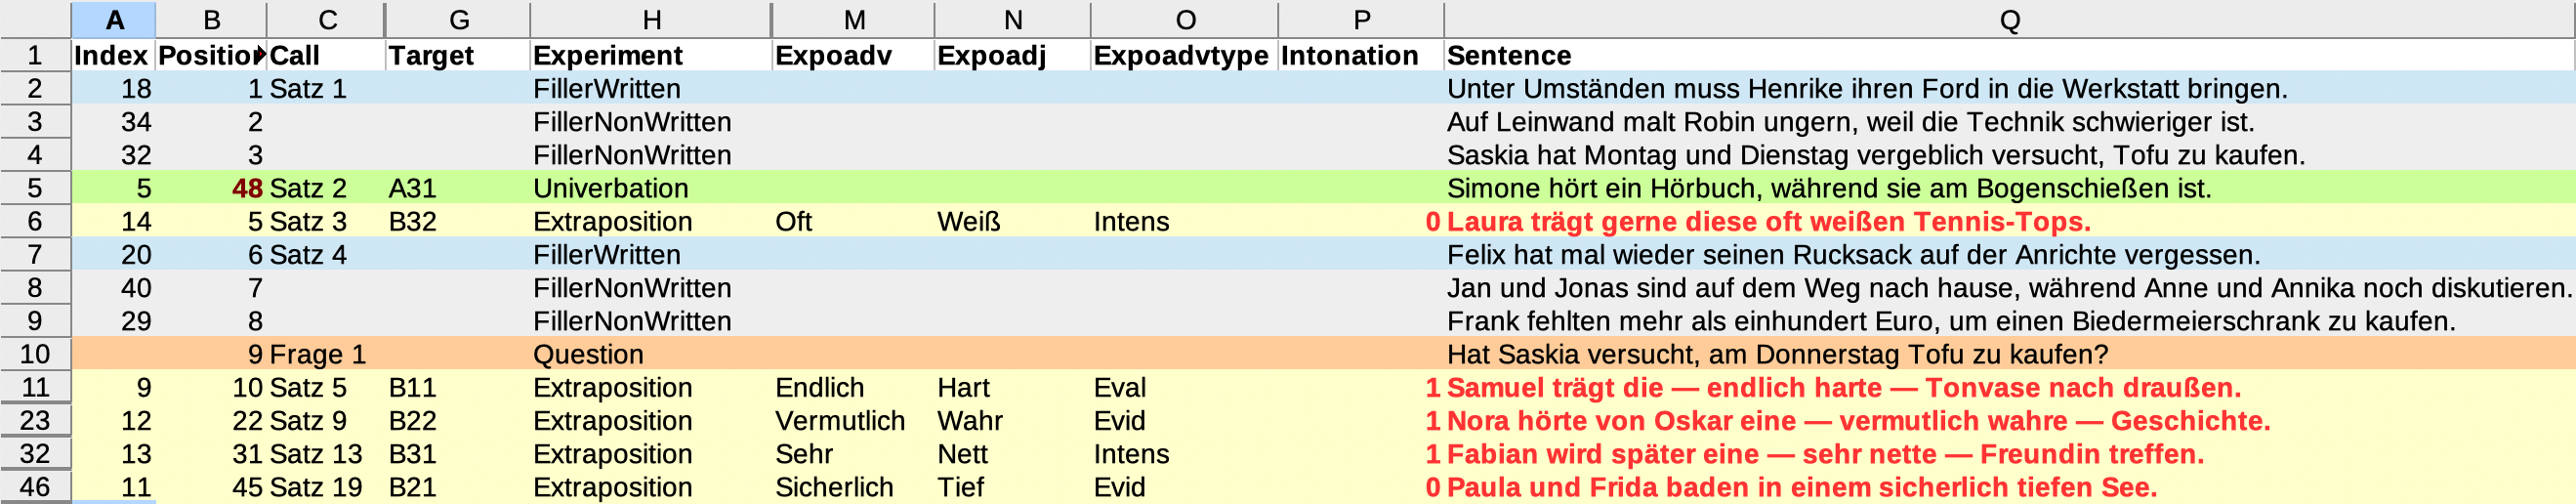
\includegraphics[width=1\textwidth]{\GRAPHPATH/Herausstellung/experiment}
\end{frame}

\begin{frame}
  {Diktatexperiment | Ergebnisse (1)}
  \centering 
  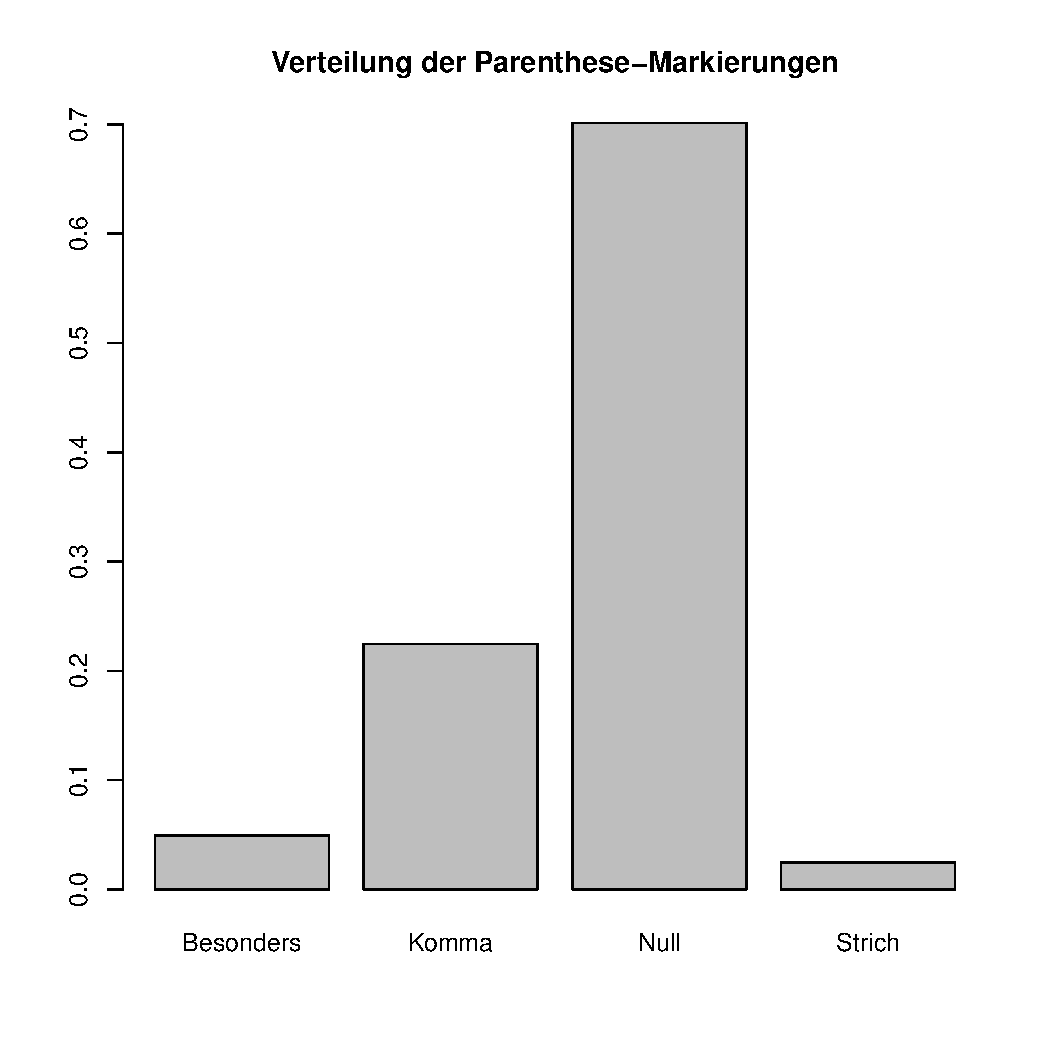
\includegraphics[width=0.5\textwidth]{\GRAPHPATH/Herausstellung/markierungen}
\end{frame}

\begin{frame}
  {Diktatexperiment | Ergebnisse (2)}
  \centering 
  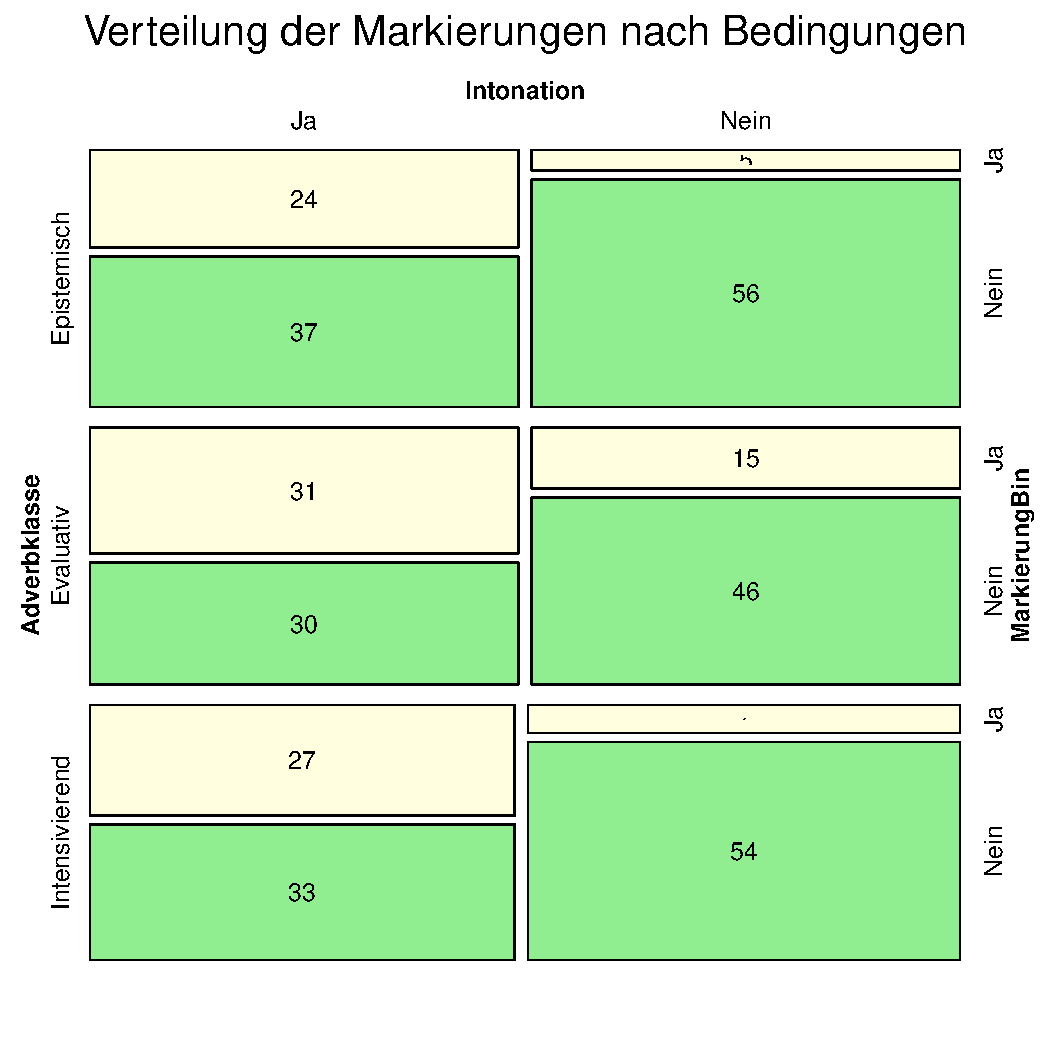
\includegraphics[width=0.5\textwidth]{\GRAPHPATH/Herausstellung/responses}
\end{frame}


\begin{frame}
  {Ergebnisse}
  \begin{itemize}[<+->]
    \item Markierung mit Komma und Gedankenstrich
    \item Komma im Experiment präferiert\\
      \grau{widerspricht Korpusstudie: über 75\% Gedankenstrich}
      \Halbzeile
    \item Intonation vertärkt Tendenz zu Markierung
    \item die Adverbklasse wirkt auch als Auslöser
      \Halbzeile
    \item Funktion?
  \end{itemize}
\end{frame}

\section[Unabhängigkeit]{Unabhängigkeit von Sätzen | \citet{SchaeferSayatz2016}}


\begin{frame}
  {\textit{obwohl} und \textit{weil} mit V2}
  \citet{SchaeferSayatz2016}\\
  \Zeile
  \centering 
  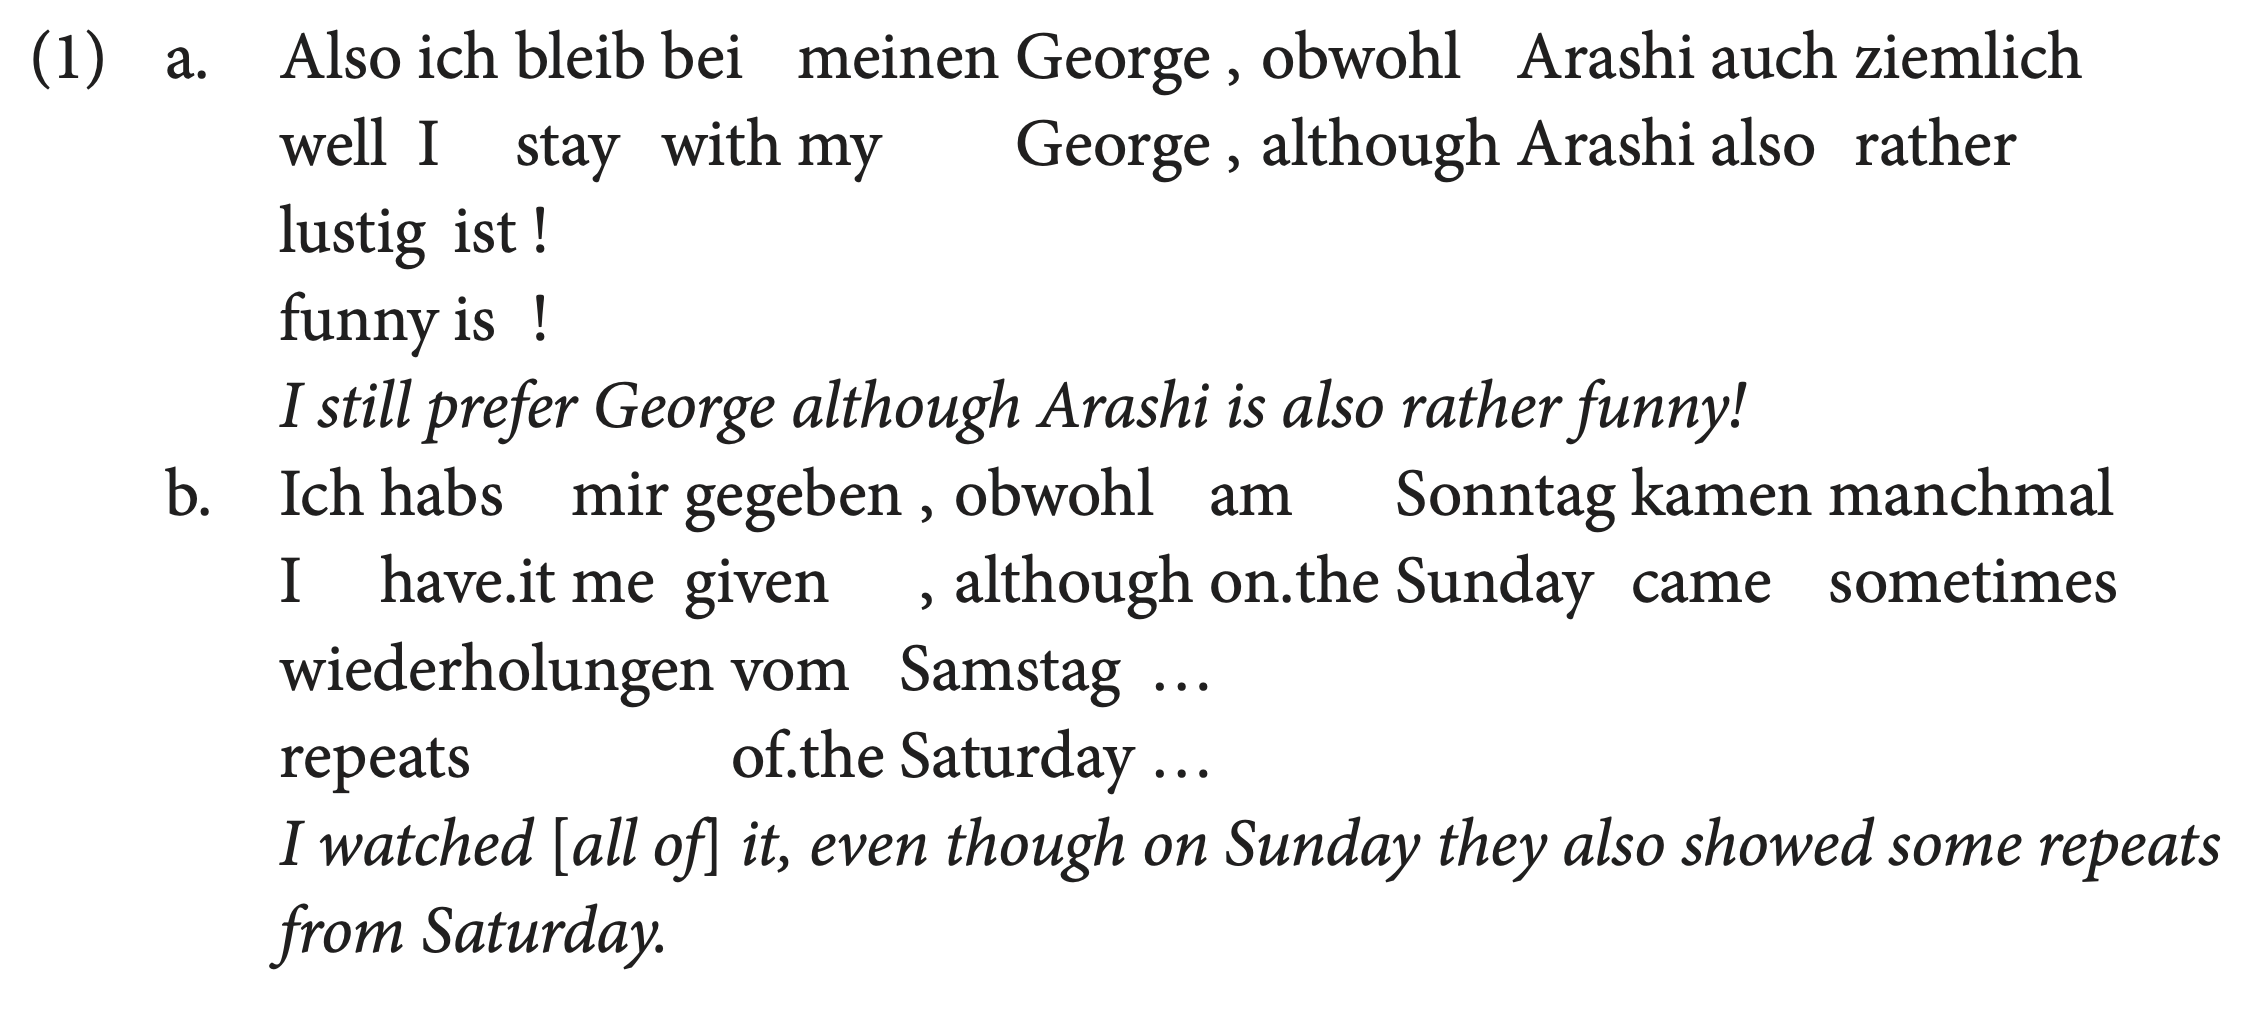
\includegraphics[width=0.7\textwidth]{\GRAPHPATH/obweil/01-obwohl}
\end{frame}

\begin{frame}
  {\textit{obwohl} und \textit{weil} mit V2}
  \centering 
  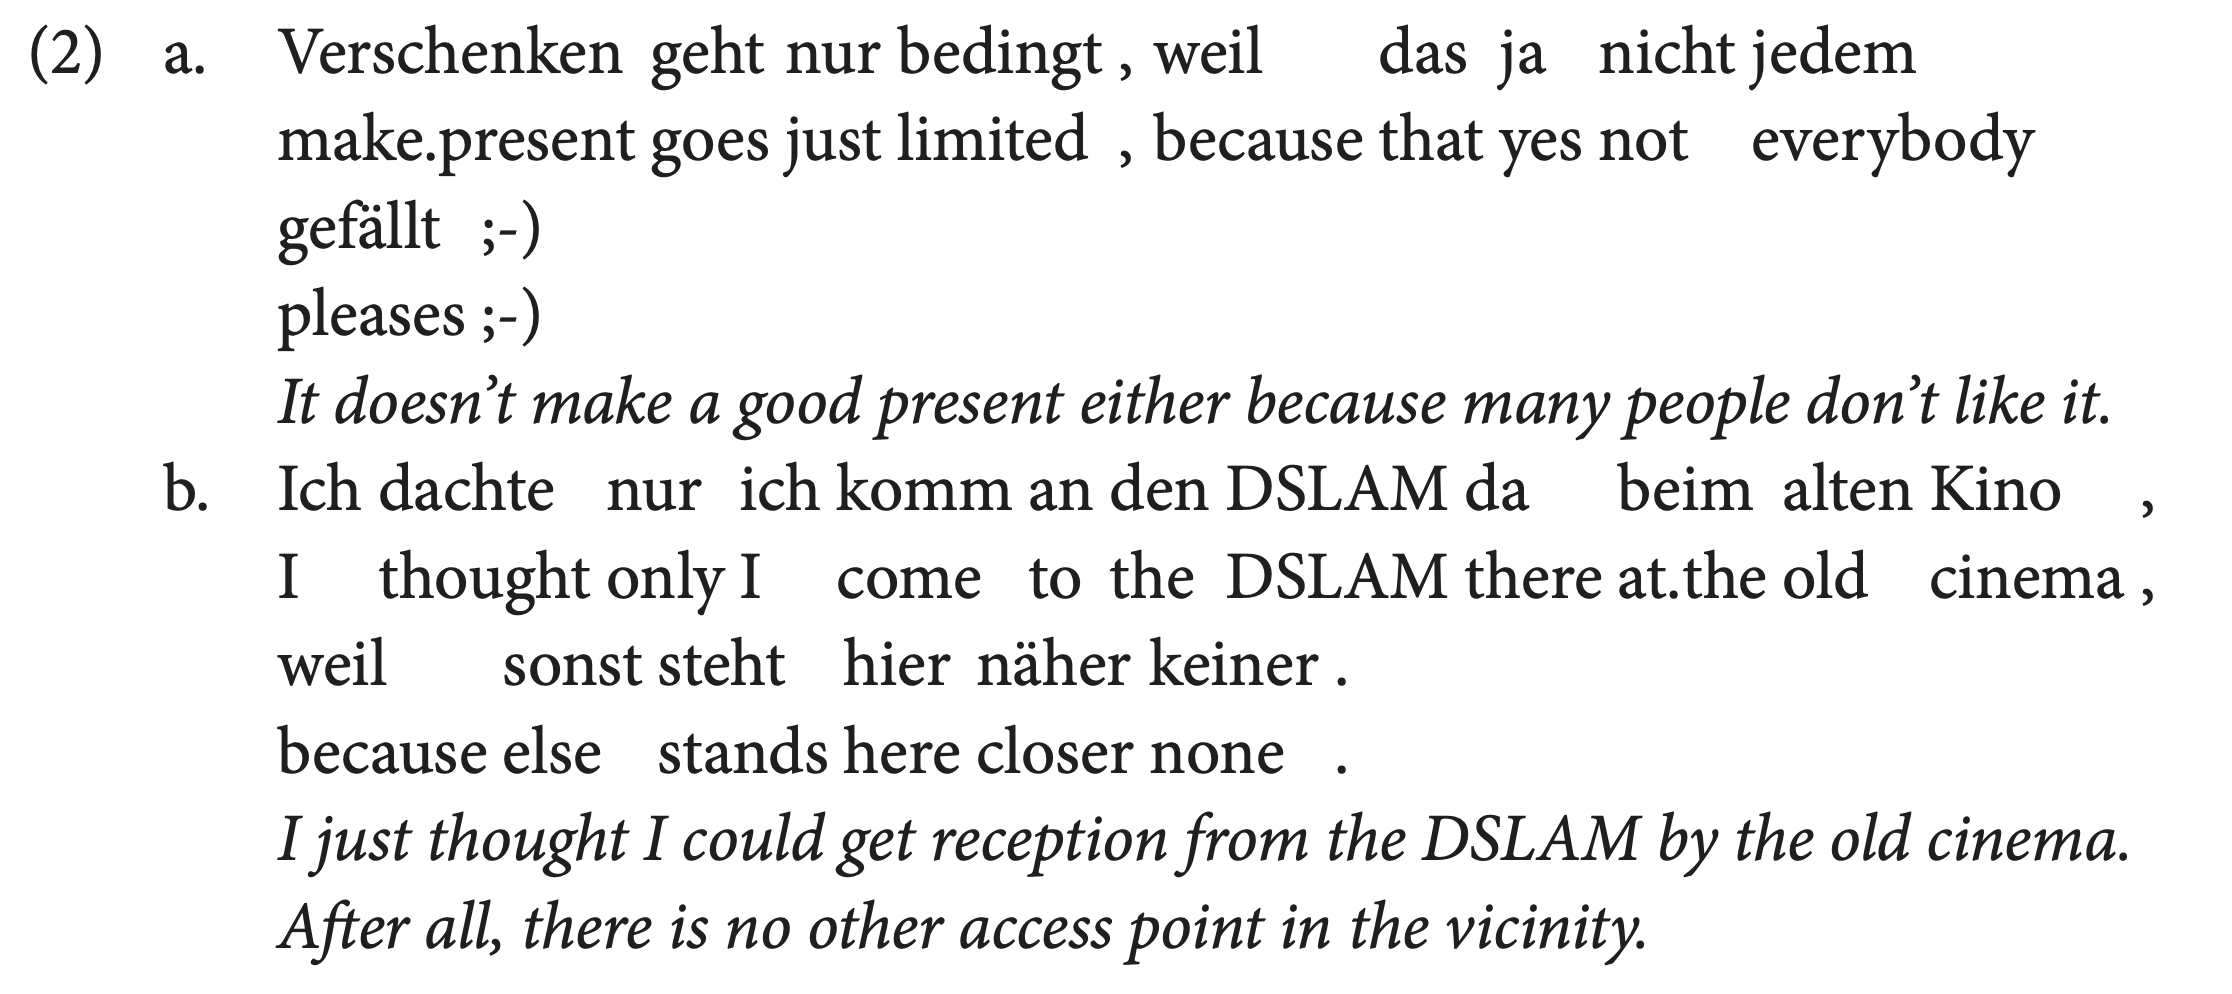
\includegraphics[width=0.7\textwidth]{\GRAPHPATH/obweil/01-weil}
\end{frame}

\begin{frame}
  {Variation der Interpunktion (Beispiele)}
  \centering 
  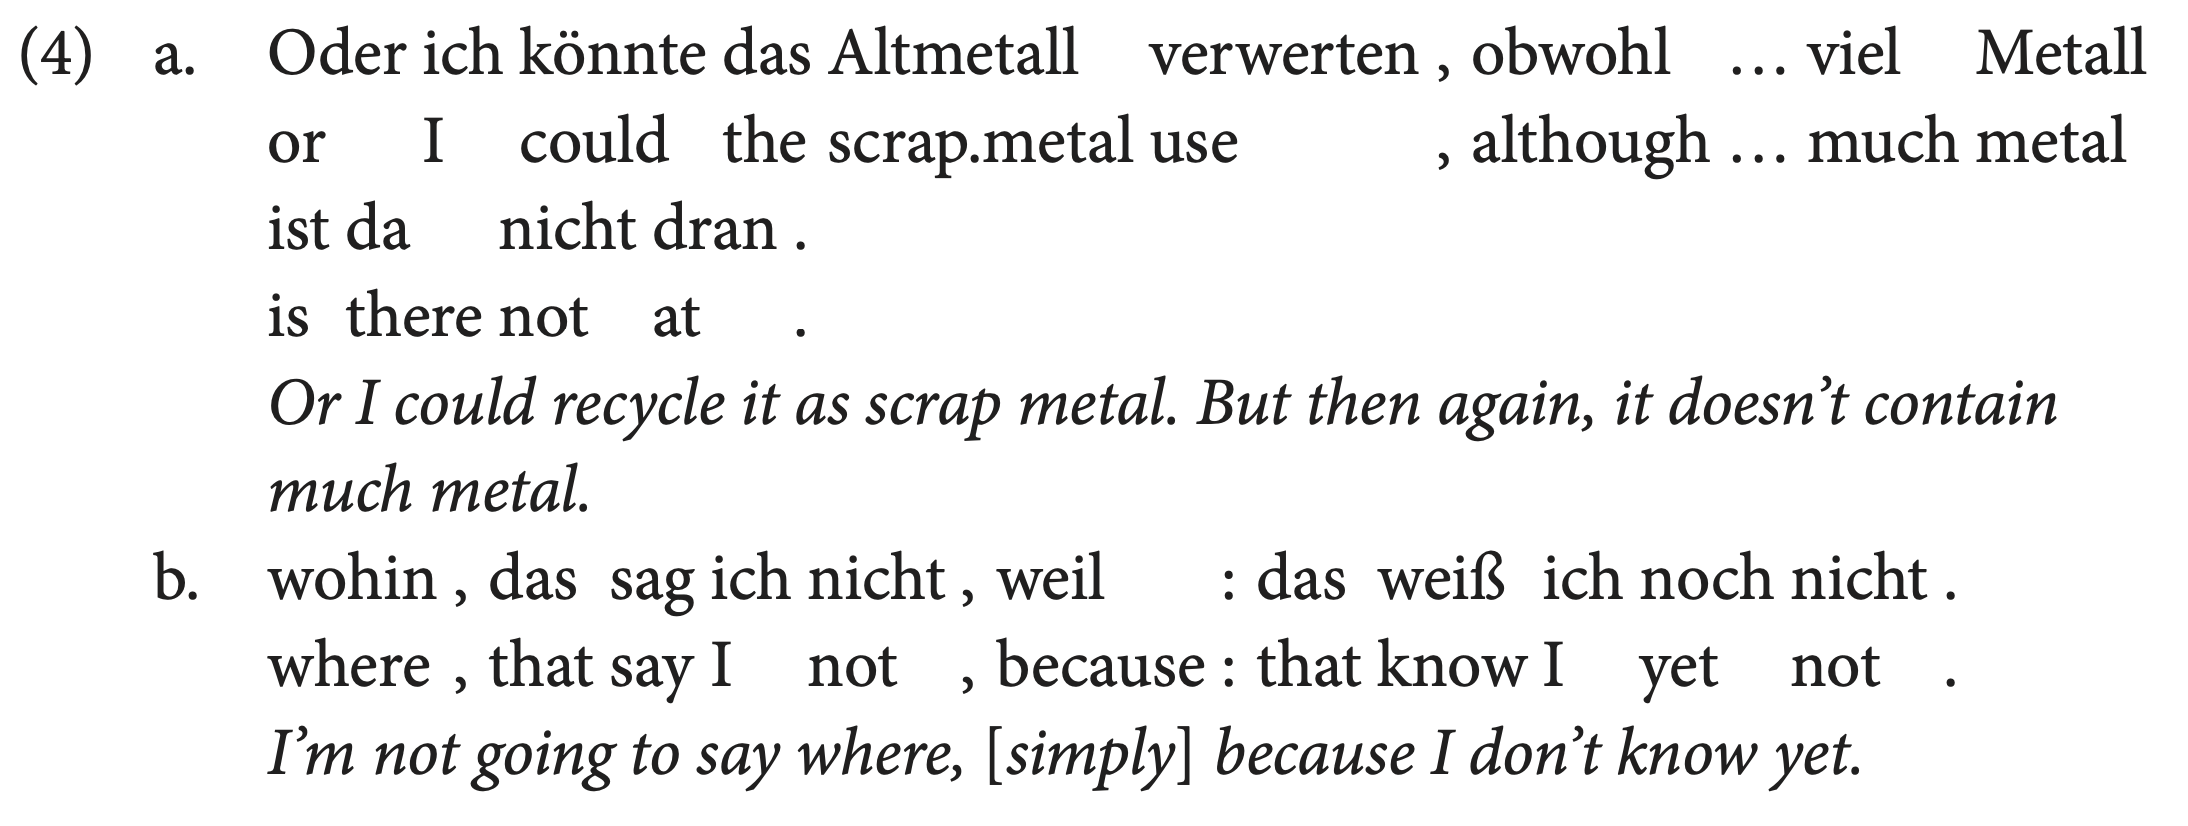
\includegraphics[width=0.7\textwidth]{\GRAPHPATH/obweil/02-interpunktion}
\end{frame}

\begin{frame}
  {Unabhängigkeit von Sätzen}
  \centering 
  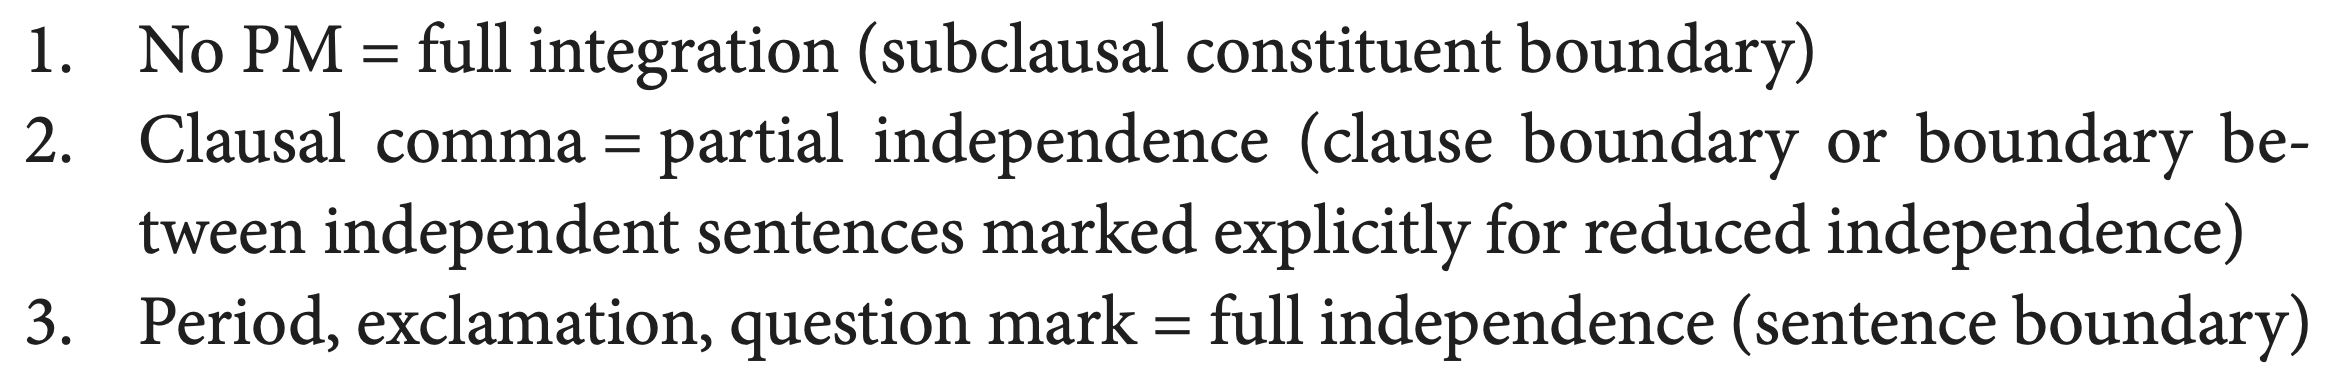
\includegraphics[width=0.7\textwidth]{\GRAPHPATH/obweil/03-independence} 
\end{frame}

\begin{frame}
  {Empirischer Befund I | Satzinitiale Partikeln}
  \centering 
  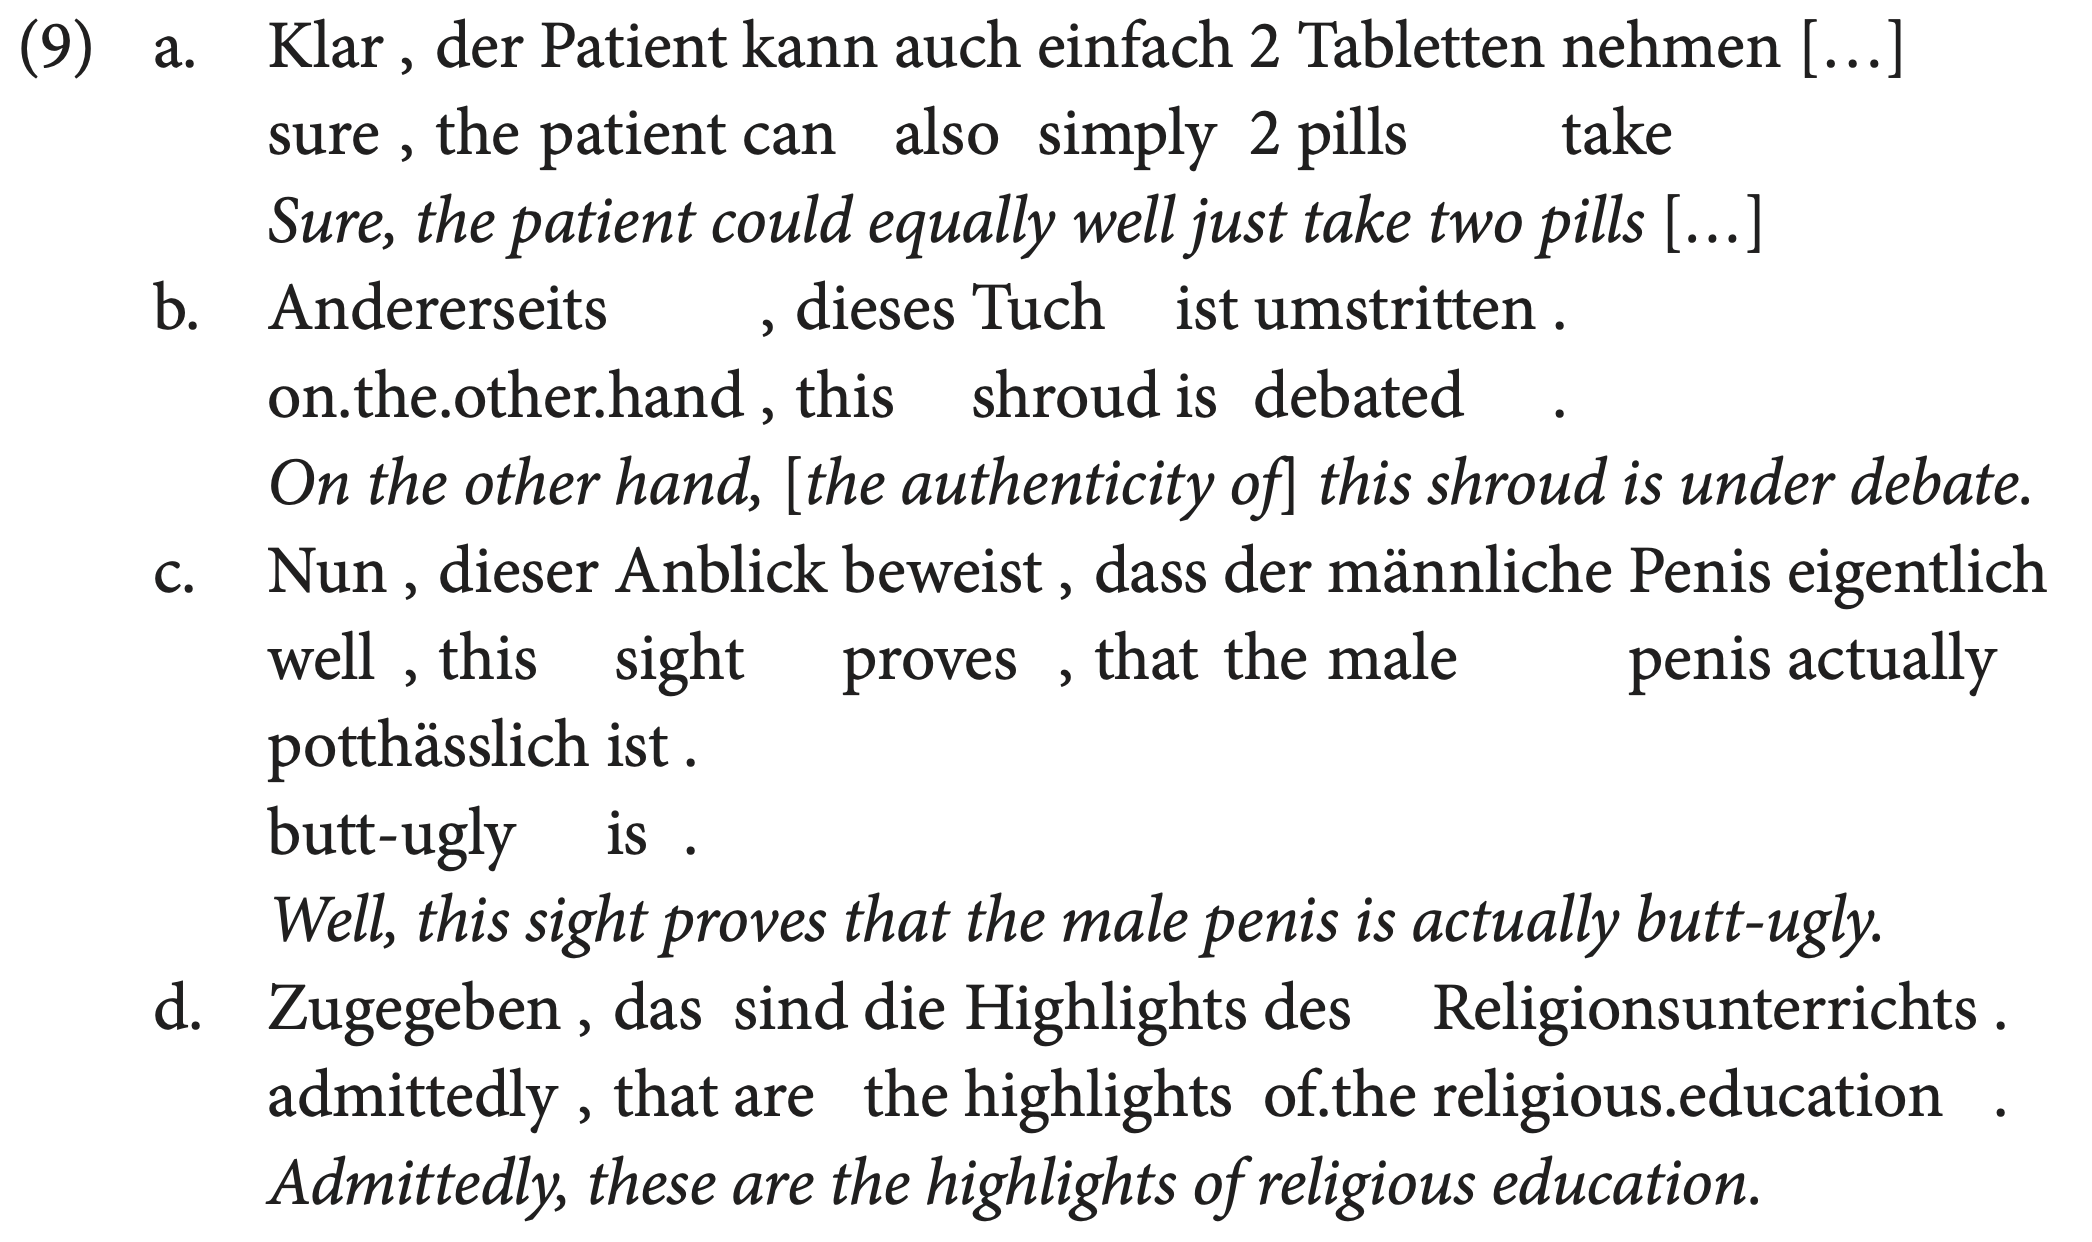
\includegraphics[width=0.7\textwidth]{\GRAPHPATH/obweil/04-satzinitial}
\end{frame}

\begin{frame}
  {Empirischer Befund II/1 | Wortverteilung bei Doppelpunkt}
  \centering 
  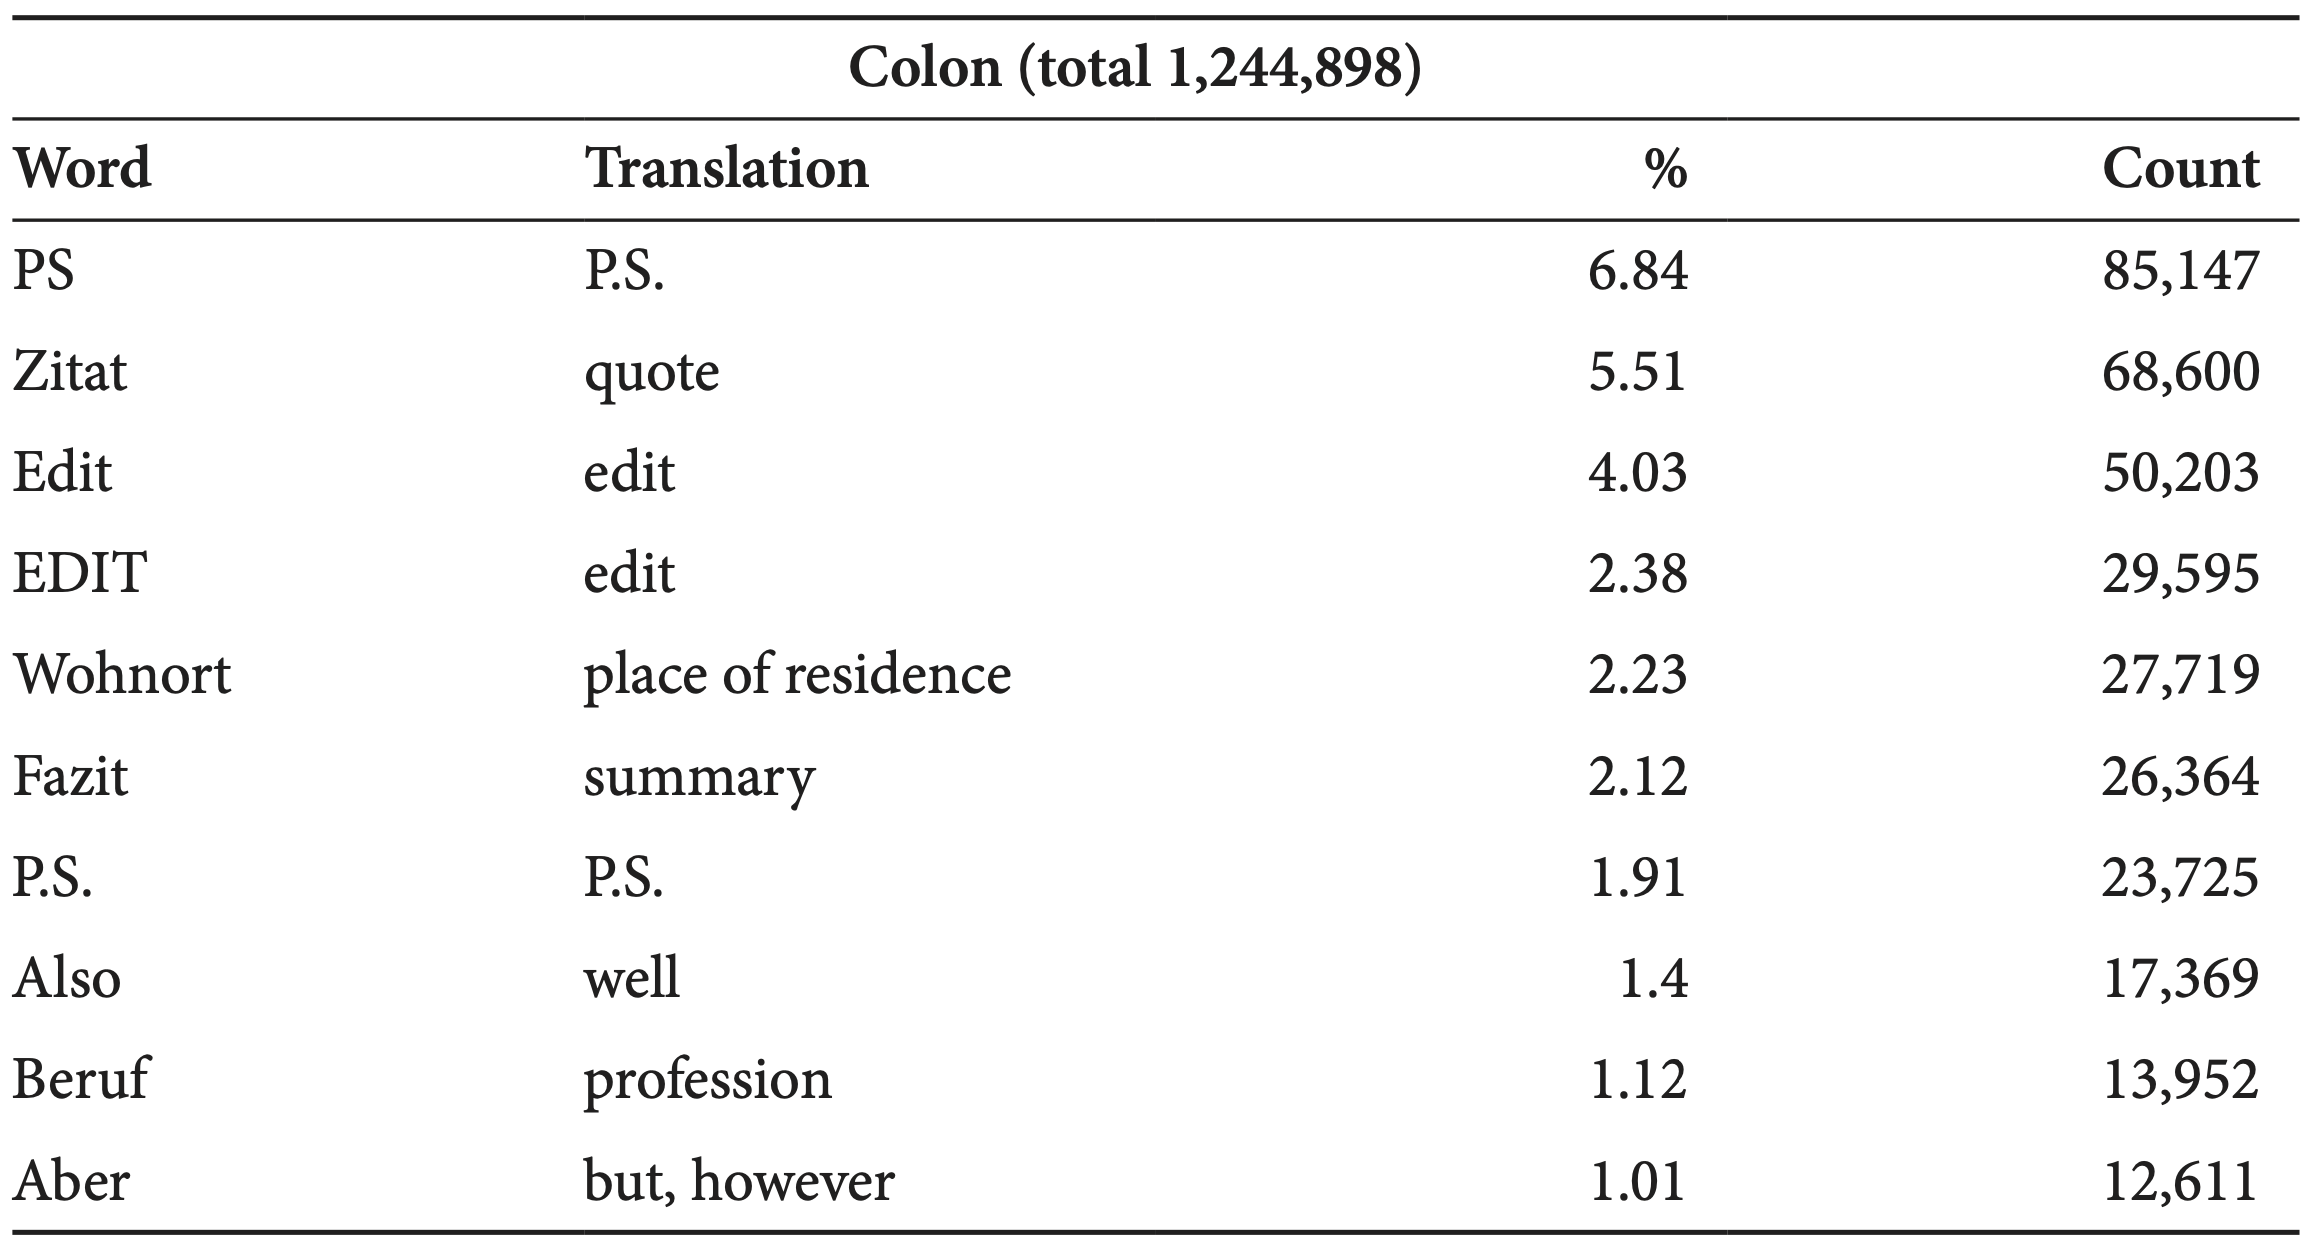
\includegraphics[width=0.7\textwidth]{\GRAPHPATH/obweil/05-colon}
\end{frame}

\begin{frame}
  {Empirischer Befund II/2 | Wortverteilung bei Komma}
  \centering 
  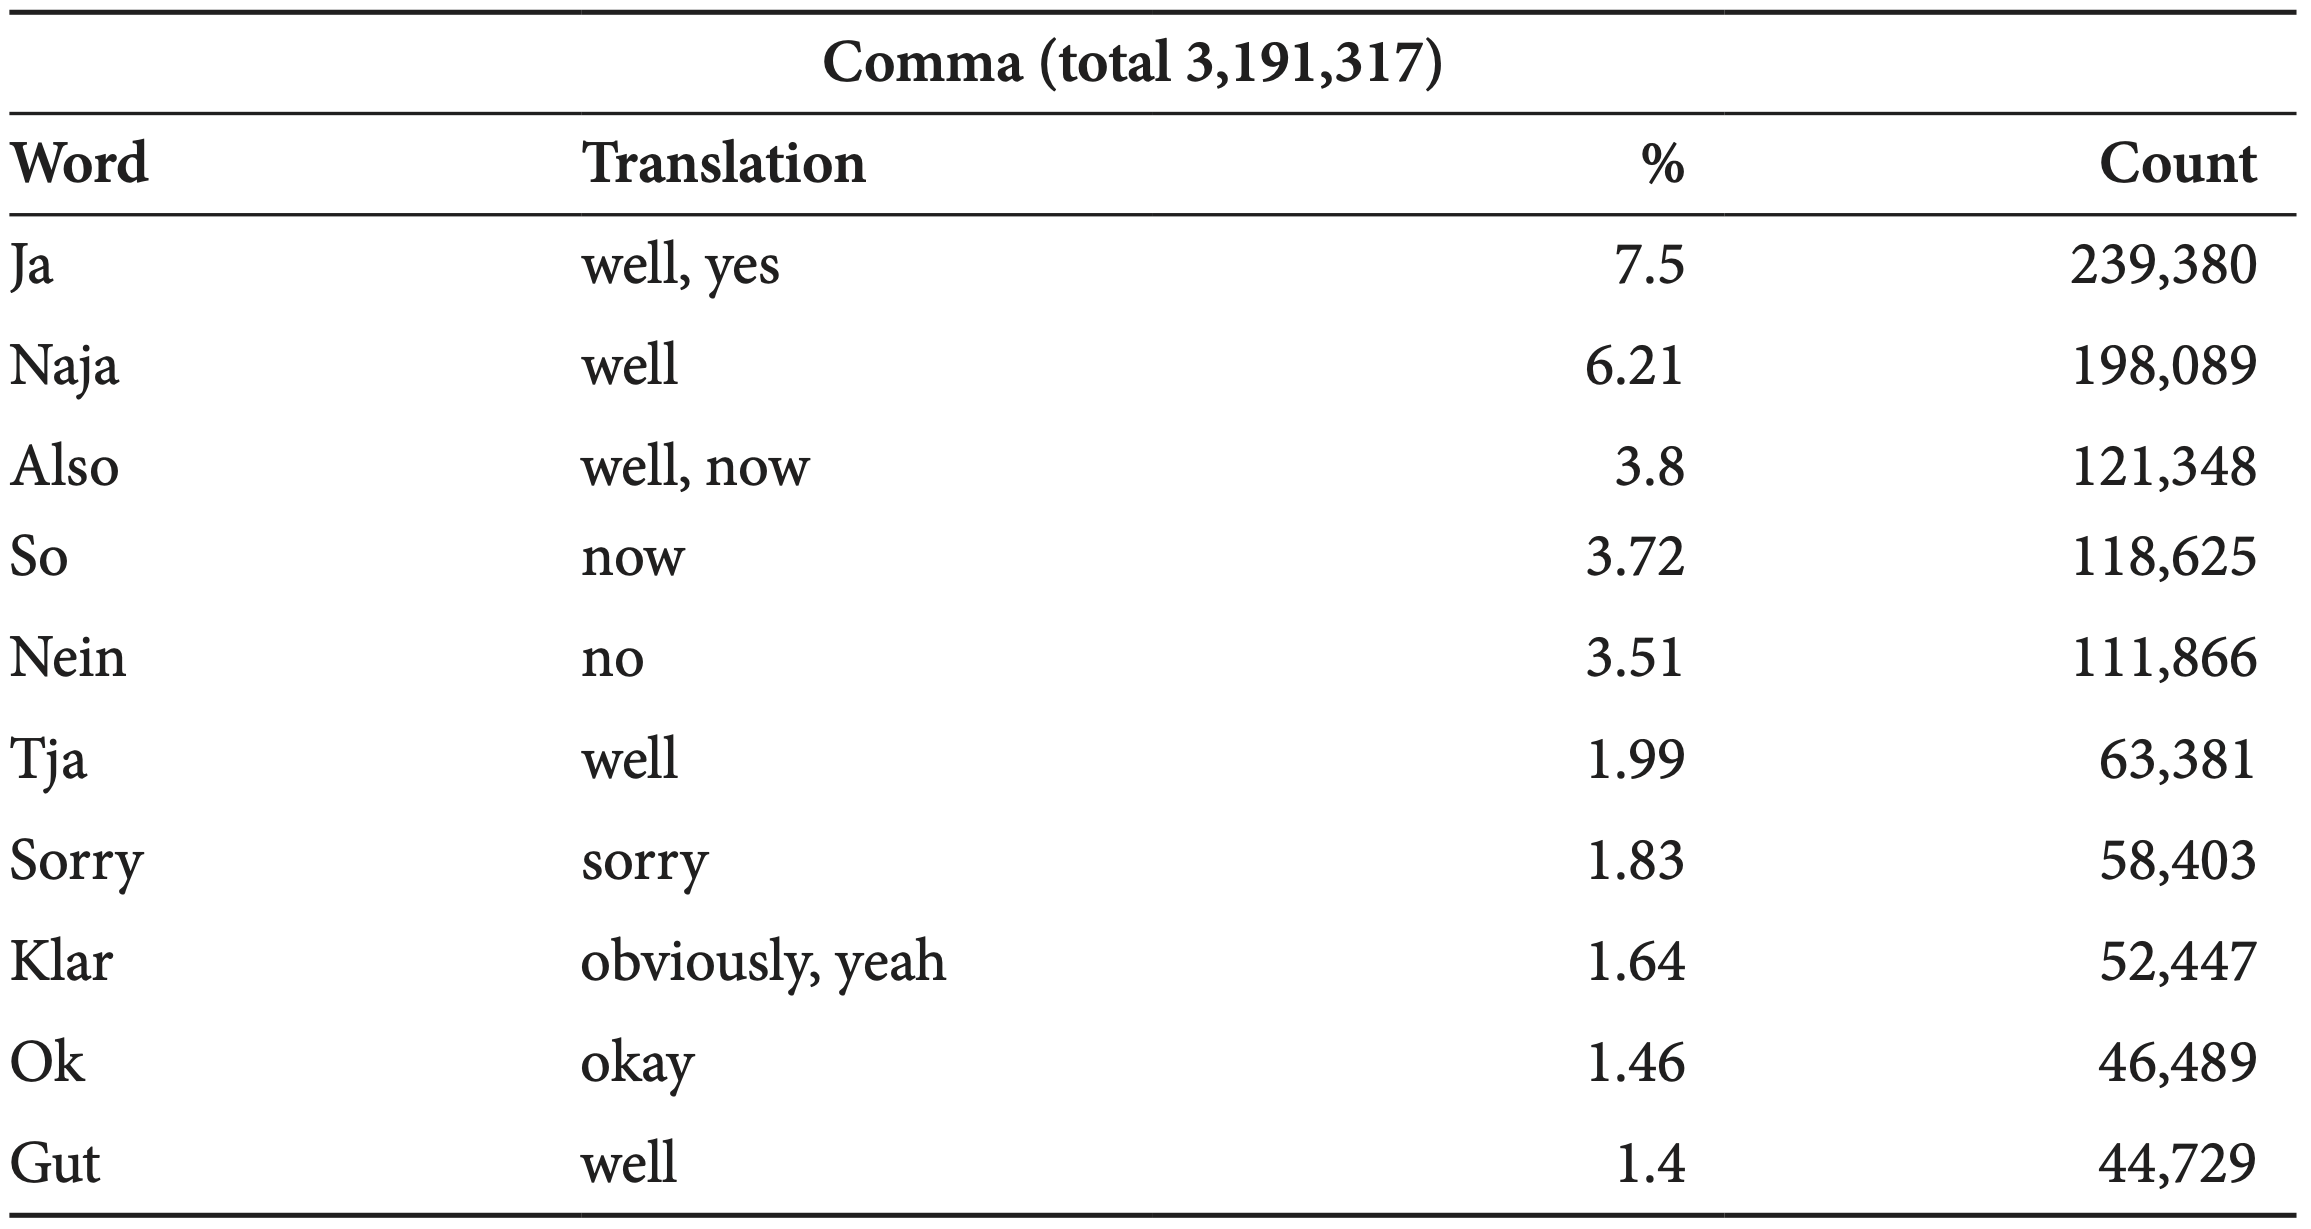
\includegraphics[width=0.7\textwidth]{\GRAPHPATH/obweil/05-comma}
\end{frame}

\begin{frame}
  {Empirischer Befund II/3 | Wortverteilung bei Bindestrich}
  \centering 
  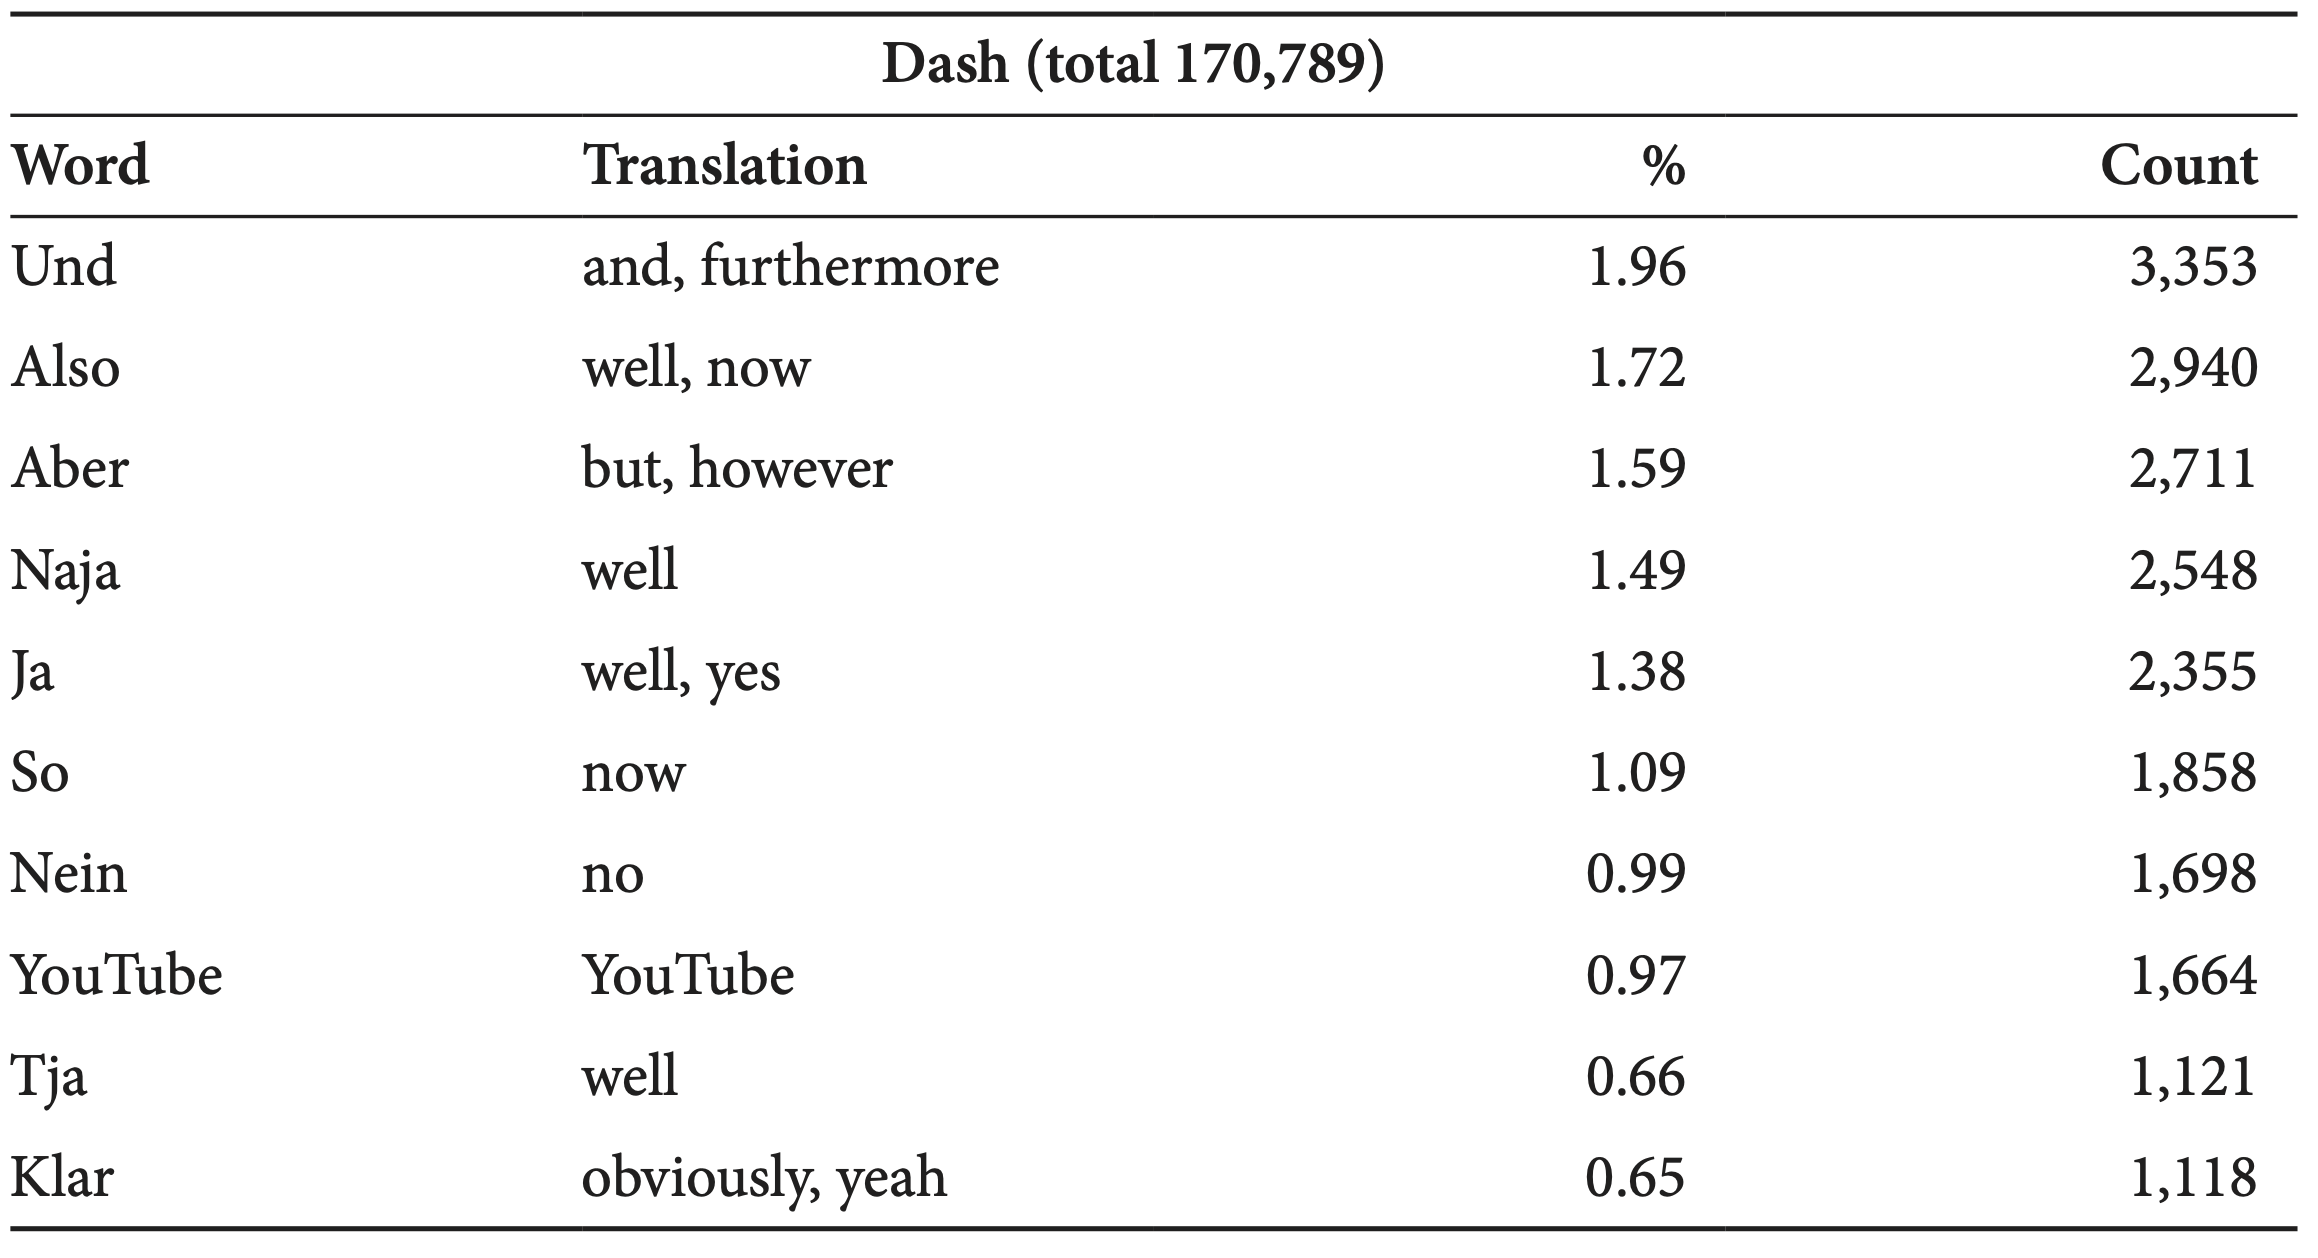
\includegraphics[width=0.7\textwidth]{\GRAPHPATH/obweil/05-dash}
\end{frame}

\begin{frame}
  {Empirischer Befund II/4 | Wortverteilung bei Dreipunkt}
  \centering 
  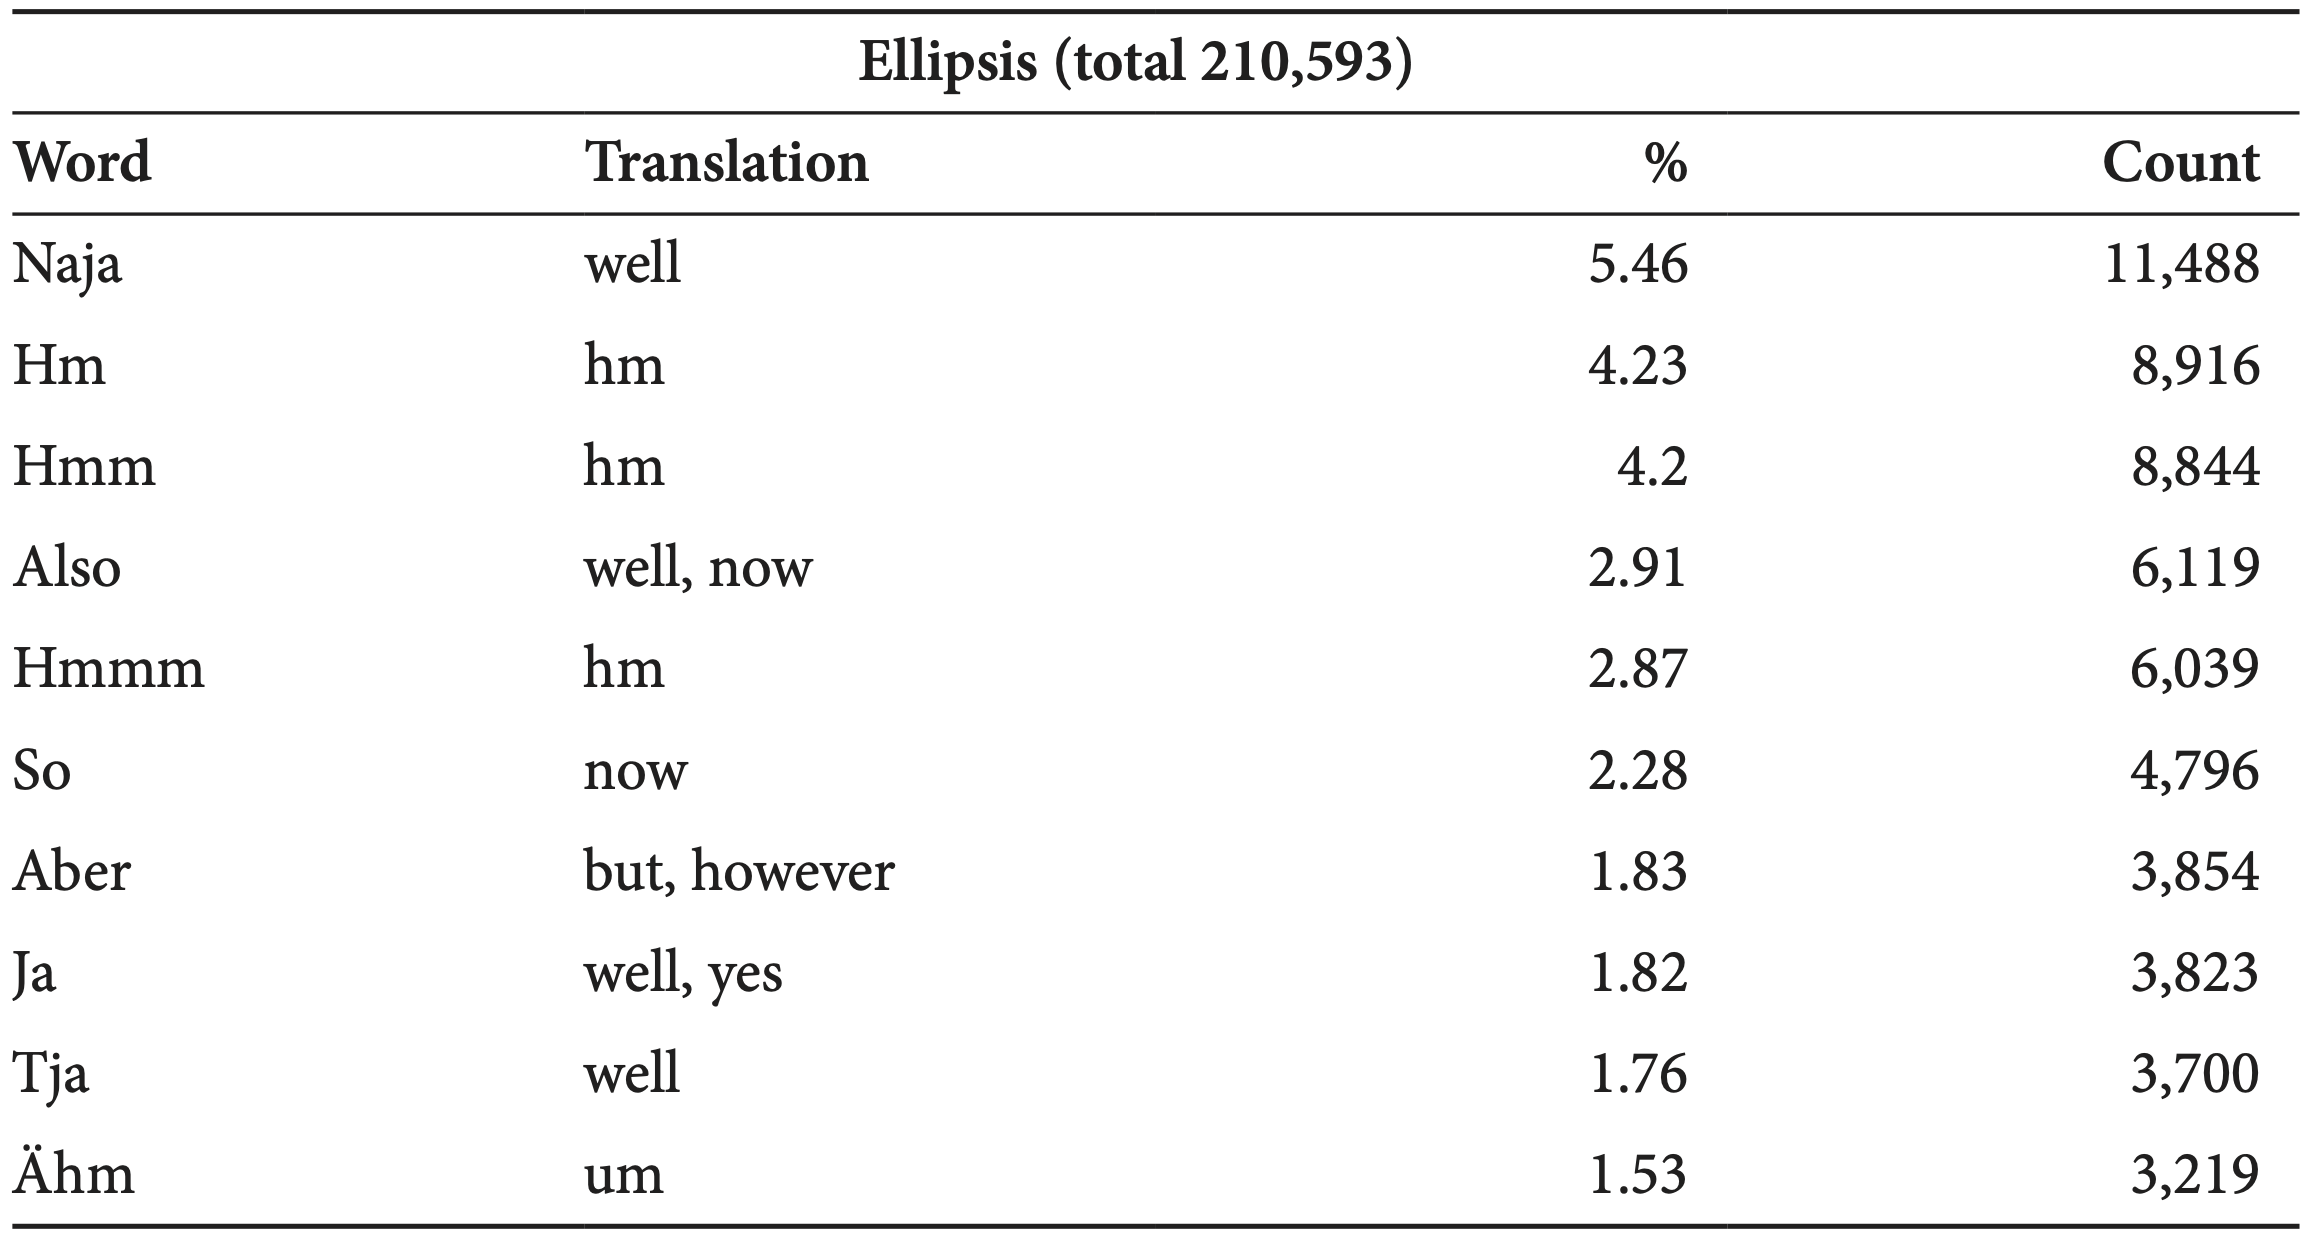
\includegraphics[width=0.7\textwidth]{\GRAPHPATH/obweil/05-ellipsis}
\end{frame}

\begin{frame}
  {Empirischer Befund III/1 | Links von \textit{obwohl}\slash \textit{weil}}
  \centering 
  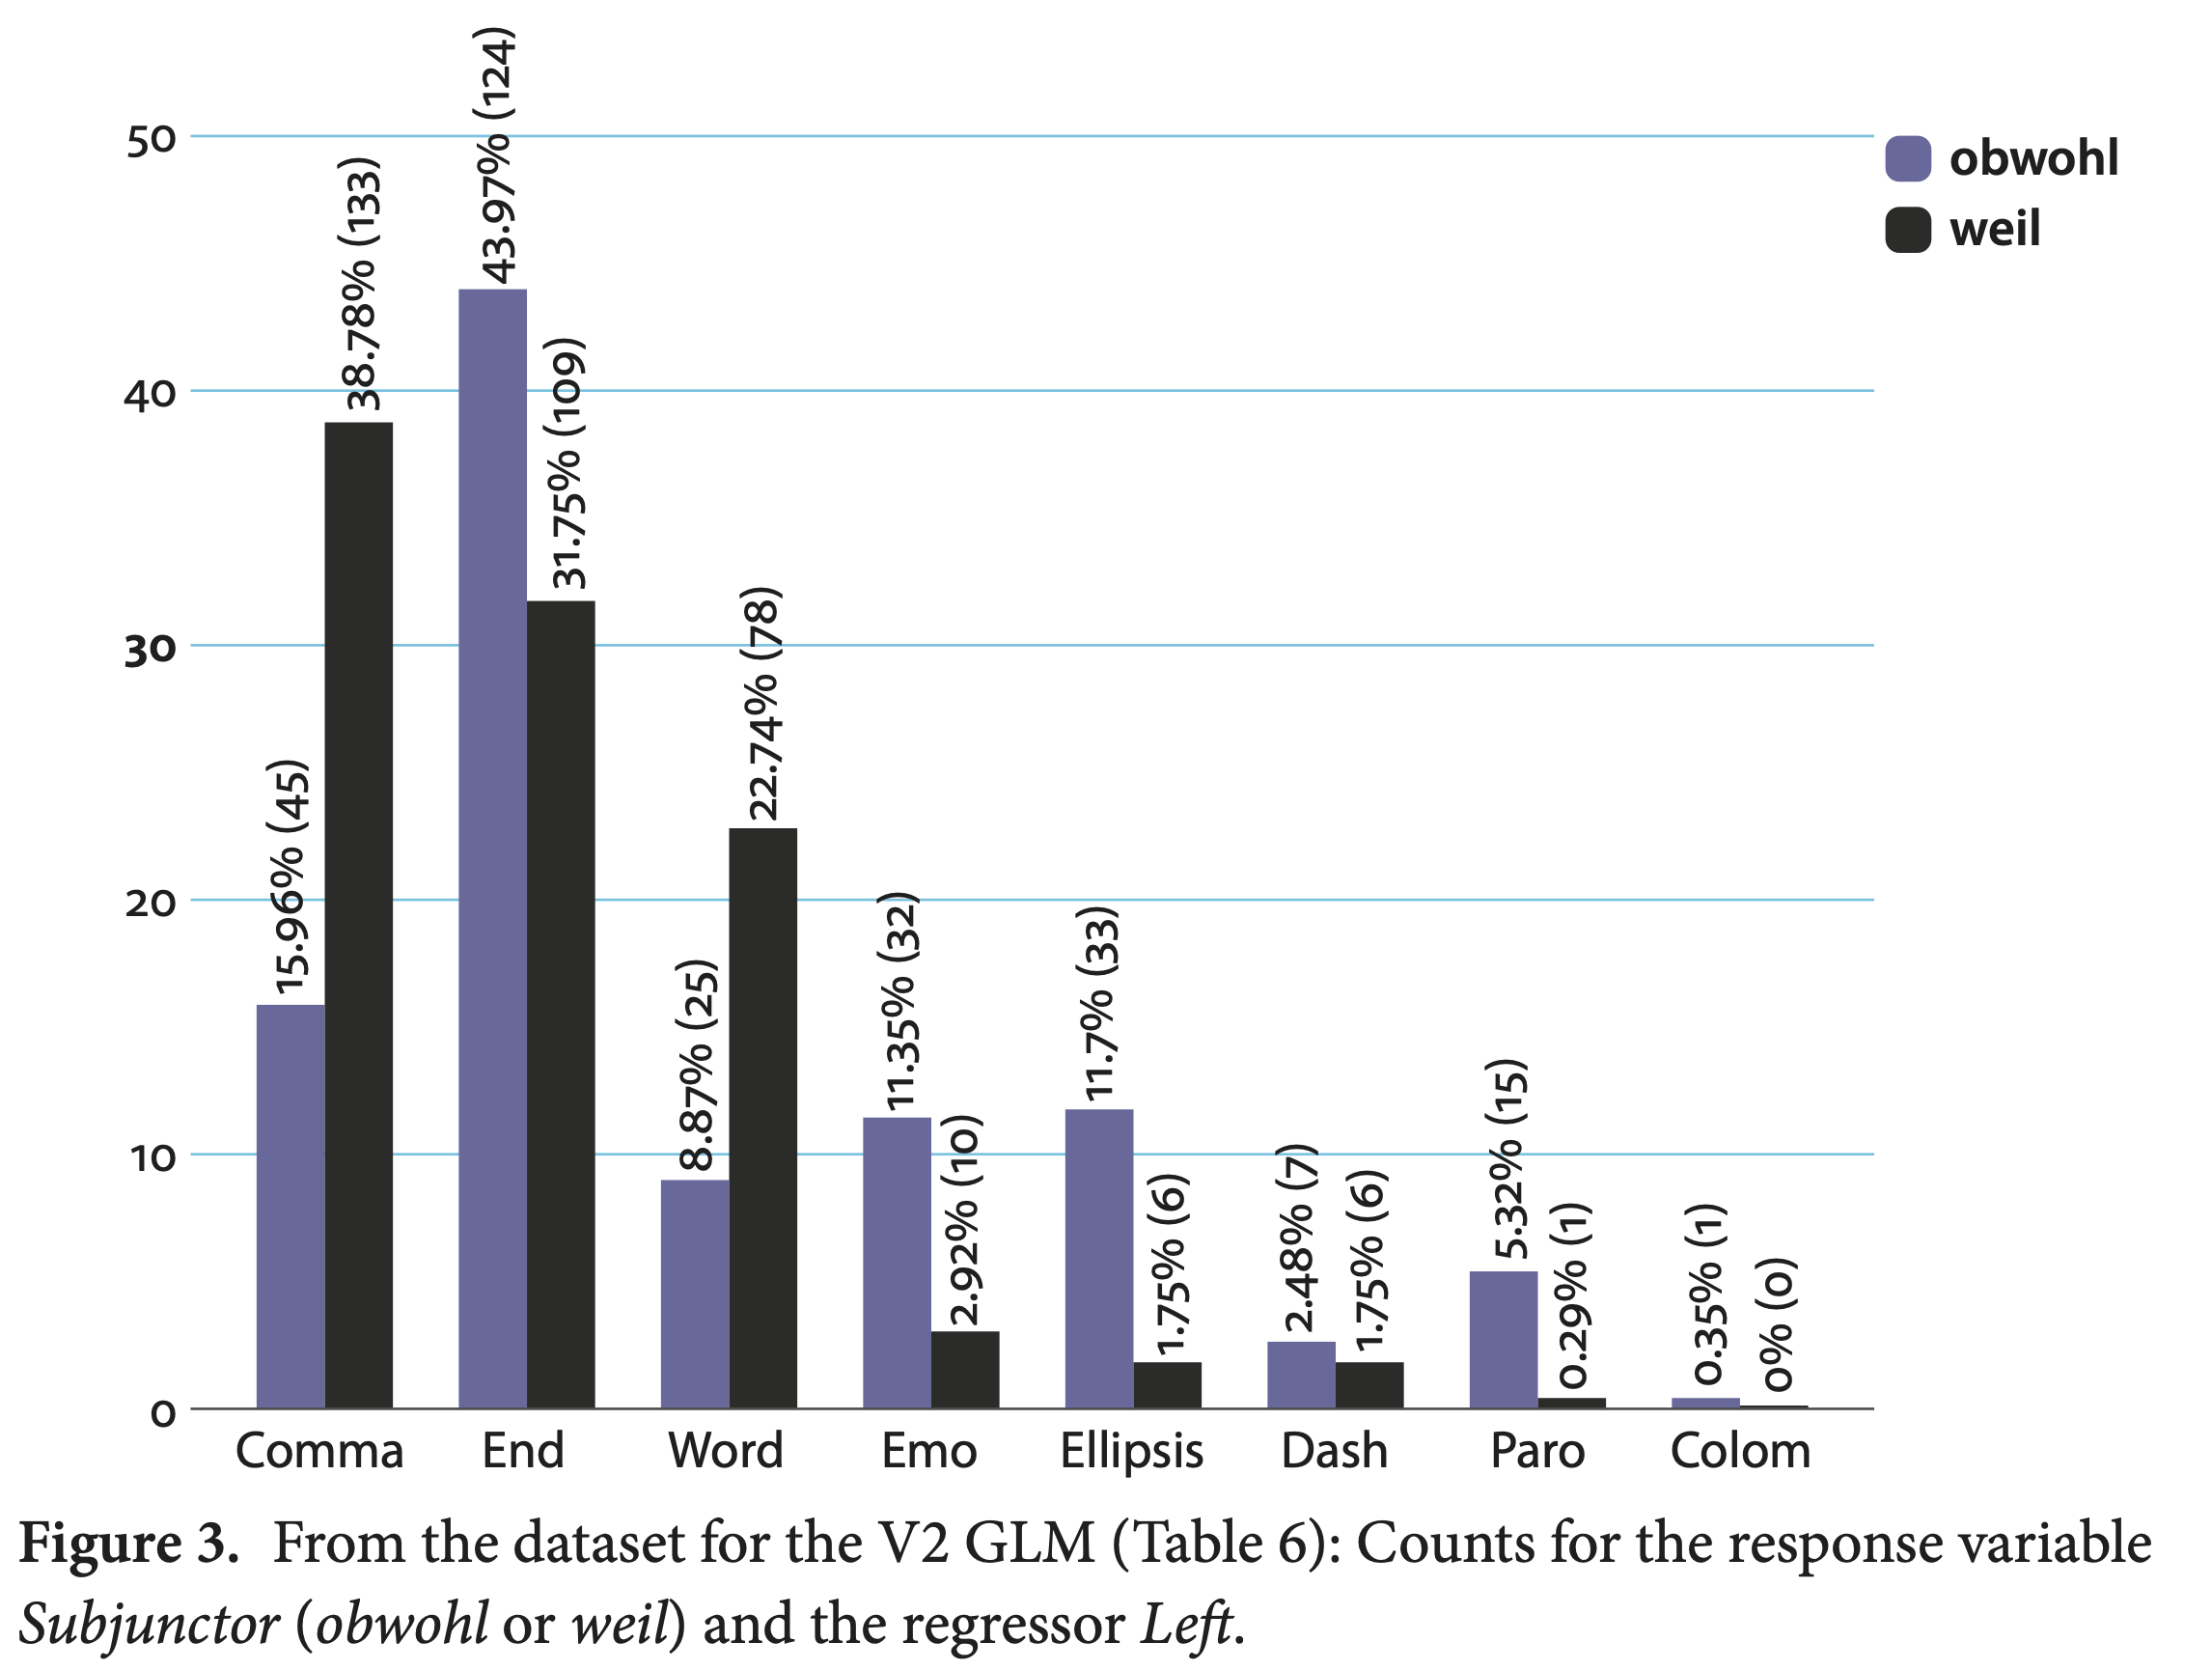
\includegraphics[width=0.7\textwidth]{\GRAPHPATH/obweil/06-left}
\end{frame}

\begin{frame}
  {Empirischer Befund III/2 | Rechts von \textit{obwohl}\slash \textit{weil}}
  \centering 
  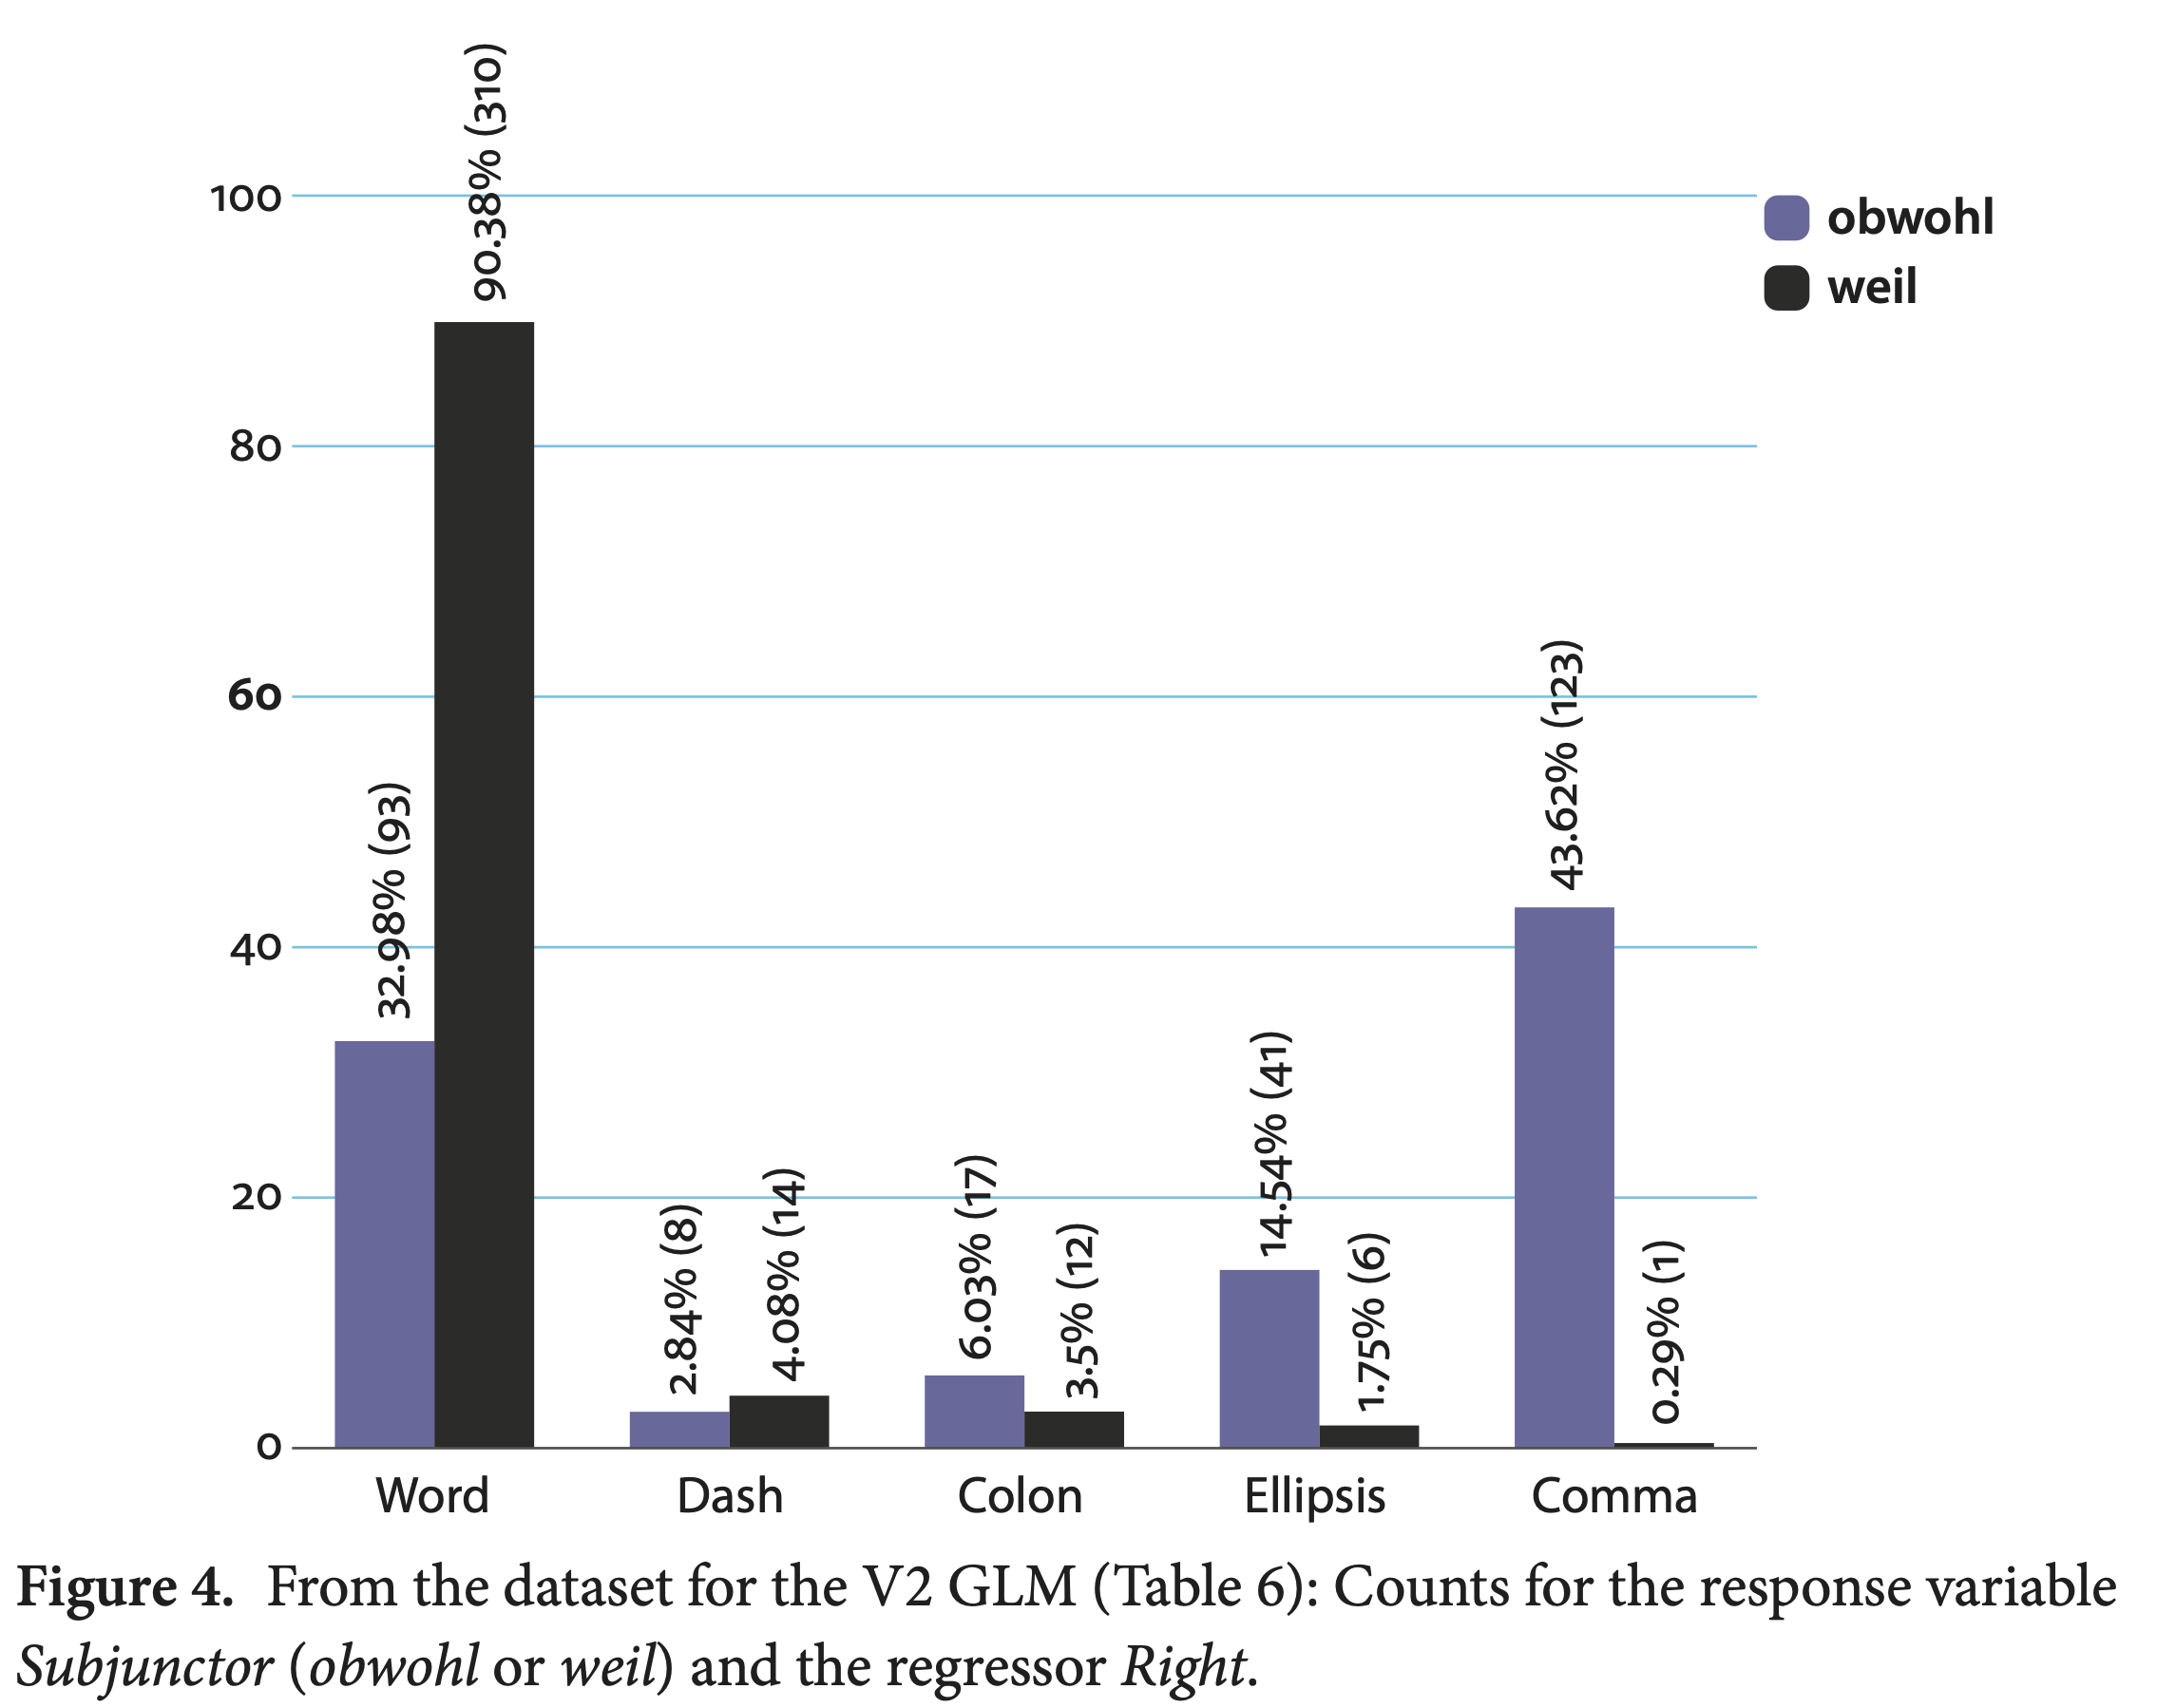
\includegraphics[width=0.7\textwidth]{\GRAPHPATH/obweil/06-right}
\end{frame}

\begin{frame}
  {Ergebnisse}
  \textit{obwohl} und \textit{weil} mit V2-Satzstellung\\
  \Zeile
  \begin{itemize}[<+->]
    \item \textit{obwohl}
      \begin{itemize}[<+->]
        \item leitet mehr unabhängige Sätze ein
        \item wird öfter vom Komma gefolgt
        \item Status | \alert{eher Diskurspartikel außerhalb des Satzes}
        \item ähnlich \textit{ja}, \textit{naja}, \textit{also}, \textit{klar}
      \end{itemize}
      \Zeile
    \item \textit{weil}
      \begin{itemize}[<+->]
        \item folgt auch bei V2 eher einem Komma
        \item oder ganz ohne Interpunktion links
        \item Komma folgt seltener
        \item Status | \alert{eher Konnektor im Konnektorfeld}
        \item ähnlich \textit{denn}
      \end{itemize}
  \end{itemize}
\end{frame}

  \let\subsection\section\let\section\woopsi
\fi

\makeatletter
\setcounter{lastpagemainpart}{\the\c@framenumber}
\makeatother

\appendix

\begin{frame}[allowframebreaks]
  {Literatur}
  \renewcommand*{\bibfont}{\footnotesize}
  \setbeamertemplate{bibliography item}{}
  \printbibliography
\end{frame}

\begin{frame}
  {Autor}
  \begin{block}{Kontakt}
    Prof.\ Dr.\ Roland Schäfer\\
    Institut für Germanistische Sprachwissenschaft\\
    Friedrich-Schiller-Universität Jena\\
    Fürstengraben 30\\
    07743 Jena\\[\baselineskip]
    \url{https://rolandschaefer.net}\\
    \texttt{roland.schaefer@uni-jena.de}
  \end{block}
\end{frame}

\begin{frame}
  {Lizenz}
  \begin{block}{Creative Commons BY-SA-3.0-DE}
    Dieses Werk ist unter einer Creative Commons Lizenz vom Typ \textit{Namensnennung - Weitergabe unter gleichen Bedingungen 3.0 Deutschland} zugänglich.
    Um eine Kopie dieser Lizenz einzusehen, konsultieren Sie \url{http://creativecommons.org/licenses/by-sa/3.0/de/} oder wenden Sie sich brieflich an Creative Commons, Postfach 1866, Mountain View, California, 94042, USA.
  \end{block}
\end{frame}

\mode<beamer>{\setcounter{framenumber}{\thelastpagemainpart}}

\end{document}
